\documentclass[11pt,a4paper]{article}
\pdfinfoomitdate=1
\pdftrailerid{}
\pdfsuppressptexinfo=15
\usepackage[T1]{fontenc}
\usepackage[utf8]{inputenc}
\usepackage{lmodern}
\usepackage[a4paper,margin=24mm]{geometry}
\usepackage{amsmath,amssymb,mathtools,booktabs,longtable,array,graphicx,microtype}
\usepackage{natbib,xurl,pdflscape,placeins,fancyvrb}
\usepackage[hidelinks]{hyperref}
\usepackage[nameinlink,noabbrev]{cleveref}
\setlength{\parindent}{0pt}
\setlength{\parskip}{4pt}
\setlength{\emergencystretch}{4em}
\allowdisplaybreaks
\hypersetup{pdftitle={AE4 salivary transport: complete mathematical analysis and model diagnosis},pdfauthor={AE4 project},pdfsubject={Source grounded technical synthesis of Tasks 43 and 44}}
\newcommand{\sourcefile}[1]{\par\smallskip{\footnotesize\textit{Source record:} \nolinkurl{#1}.}\par}
\newcommand{\reportnote}[1]{\par\smallskip\textbf{Interpretation.} #1\par\smallskip}
\begin{document}
\begin{titlepage}
\centering
\vspace*{18mm}
{\Large AE4 salivary transport\par}
\vspace{8mm}
{\huge\bfseries Complete mathematical analysis, parameter provenance and diagnosis of model inadequacy\par}
\vspace{12mm}
{\Large Technical report based on the completed Codex Tasks 43 and 44\par}
\vspace{10mm}
{15 September 2026\par}
\vfill
\begin{minipage}{.94\textwidth}
This report consolidates the completed analysis of the frozen Task 40 model and the prescribed Task 41 inverse family. It includes the full mathematical exposition, expanded computational methods, complete numerical case tables, parameter provenance and the original electronic evidence. It is a technical basis for article development, not a new model or a claim that the biological mechanism has been validated.

\medskip
\textbf{Immutable scientific inputs}\par
Task 43: \nolinkurl{547f113d9123ab1976774639a69483faf40cef34}\par
Task 44: \nolinkurl{e5fa9840bf96be3147c6118daee4942468c78f8b}\par
Numerical replay: \nolinkurl{f783785a863440df459e9c5530beba4c7eb59110}

\medskip
The source branches, production code, original outputs and existing manuscript are not modified by this report. Exact results, local numerical findings, finite duration calculations and unresolved biological questions are explicitly distinguished.
\end{minipage}
\end{titlepage}
\begin{abstract}
The reconstructed AE4 salivary transport model was examined using complete parameter provenance, invertible nondimensionalisation, conditional algebraic closure results, conserved amount identities, equilibrium continuation, local stability and sensitivity analysis, source vector projections and an inverse CaCC recruitment calculation. Carbon, alkalinity, both finite volumes, lumen composition, algebraic pH and electrical closure, and AE4 regulation remain present. Thirteen production states are represented by eleven independent dynamic coordinates after exact charge elimination. At the frozen parameter point the stationary AE4 null secretion deficit is approximately 0.94617\%, while the original 600 s cumulative deficit is 3.8575\%. Local NKCC chloride compensation is approximately 92.901\%; the integrated replacement of missing AE4 chloride over 60 to 600 s is 88.507\%. These are distinct observables. The system already contains slow modes of approximately 346 and 460 s in WT and null. A physiological NBC absent root exists at much lower AE4 loading, so the alkalinity obstruction is conditional on a specified loading demand. The prescribed Task 41 family requires approximately 89.51\% AE4 dependent stimulated CaCC recruitment at its first numerical comparison crossing, but that target selected construction later violates the pH gate. The analysis diagnoses a mismatch between a particular mathematical reconstruction and the biological phenotype. It does not prove that NKCC1 is the unique defective component, that compensation must vanish in all protocols, or that a better model has already been identified. Full source attribution and electronic numerical evidence accompany the technical account.
\end{abstract}
\clearpage
\tableofcontents
\clearpage
\part{Purpose, interpretation and computational methods}
\section{Question, scope and standard of inference}
\label{sec:report-scope}
The scientific question is why AE4 loss produces a substantial sustained salivary secretion deficit even though NKCC1 remains available as a chloride loading pathway, whereas AE2 loss has comparatively little effect in the experimental comparison. The work documented here did not construct a successful replacement model. It analysed a particular conservation explicit reconstruction and established exactly how that reconstruction responds to AE4 perturbation. The distinction matters: a mathematically coherent response can still be an inadequate account of the biological experiment.

The main mathematical input is the completed Task 44 analysis, including its final report, all included TeX fragments, numerical tables, verification records and executable analysis scripts. The parameter input is the completed Task 43 audit. Their final branch commits are pinned on the title page. Both refer to the frozen Task 40 production configuration; Task 44 additionally examines the single Task 41 CaCC recruitment family. Earlier Tasks 37 to 42 supply the frozen reference context. Task 46 model discovery is outside the scope of this report, and no prospective candidate is treated as a result.

This is a source grounded synthesis. Part II retains the complete Task 44 mathematical exposition, rather than replacing it by a summary. Part III retains the completed Task 43 provenance account. Part IV supplies the full equilibrium case tables, spectra, modal contributions, expression sensitivities, all extended parameter sensitivity metrics, inverse scan and both inverse sensitivity observables, followed by detailed parameter records. Part V explains verification, coverage and the implications for article development. The accompanying electronic archive contains the original reports, scripts and machine readable payloads unchanged, with an individual hash manifest. Large arrays, all nearby trial records and per diagnostic residuals are preserved there rather than rounded into a few headline numbers.

\subsection{Four levels of conclusion}
An \emph{exact or proved} result follows from the stated equations under its explicit domain assumptions. It need not hold after a kinetic law, charge convention or transported source vector is changed. A \emph{local numerical} result describes a solved equilibrium, derivative or spectrum at a specified parameter point. It is not a proof of global uniqueness or a statement over unknown physiological parameter ranges. A \emph{finite duration numerical} result describes an initial condition, stimulus, integration method and observation window. It is not an equilibrium statement. An \emph{unresolved} issue is one for which the existing sources do not establish the proposed conclusion. The completed analysis contains all four categories, and the report does not promote one into another.

In particular, repeated numerical reproduction establishes consistency of a computation with its saved inputs. It does not independently validate the biological mechanism. Similarly, a physiological gate is an inherited admissibility criterion used in this investigation, not a newly measured confidence interval. A case can pass these gates while having a separate thermodynamic qualification.
\sourcefile{evidence/task44/FINAL_STATUS.md; evidence/task44/report.tex; evidence/task43/FINAL_STATUS.md}

\section{What system was actually analysed?}
\label{sec:report-state}
The production model represents an acinar cell, a finite lumen and a fixed extracellular bath. Its thirteen evolving coordinates are the five intracellular amounts of sodium, potassium, chloride, total inorganic carbon and total alkalinity, the cell volume, the corresponding five luminal amounts, the lumen volume and an AE4 regulatory fraction. The fixed bath is an external reservoir; the lumen has an outflow sink. Consequently, conservation means that every internal and boundary source is accounted for. It does not mean that each amount in the open cell and lumen is individually constant.

Total inorganic carbon is the sum of carbon dioxide, bicarbonate and carbonate. Alkalinity records bicarbonate, twice carbonate, the deprotonated noncarbonate buffer, hydroxide and the negative contribution of hydrogen. Internal protonation changes speciation but does not create total inorganic carbon or alkalinity. Proton extrusion and bicarbonate or carbonate transport have different source signatures. Retaining those signatures is central to the analysis, rather than a cosmetic reformulation of a chloride model.

At each evaluation, carbonate equilibrium determines pH and species concentrations from amounts and volume. The electrical equations determine apical and basolateral voltage from the current balance. Neither pH nor voltage is an independently frozen constant. Water flow responds to the current osmotic state, and lumen outflow removes both water and solutes. AE4 regulation remains dynamic. The calcium stimulus is prescribed, not generated by a calcium signalling subsystem.

Two charge identities permit exact elimination of the two alkalinity coordinates from the numerical independent state. This changes thirteen stored production coordinates into eleven independent dynamic coordinates, without discarding the alkalinity balances or their effects. In particular, the eliminated intracellular alkalinity is reconstructed from sodium, potassium, chloride and fixed anion amount; luminal alkalinity is reconstructed from luminal ionic charge. This is not the reduction in \texttt{Marty.tex}. No carbon pool, volume or luminal composition has been held constant to obtain the eleven dimensional system.

The independent representation is important for equilibrium differentiation. Keeping redundant charge coordinates would introduce directions that do not represent freely variable dynamics on the analysed charge manifold. The computed nonsingularity and stability statements refer to that manifold and the declared regulatory linearisation, not to an unconstrained enlargement of the model.

\subsection{Notation used in the inherited analysis}
The mathematical chapters use $N$ for NKCC1 cycle flux, $H$ for NHE1 flux, $E$ for AE2 flux, $B$ for NBC cycle flux, $J_4$ for AE4 cycle flux, $P=P_a+P_b$ for pump cycle flux, and $C_a$ for apical chloride efflux. The symbol $H$ used as a flux must not be confused with hydrogen concentration, which is written $h$ or $[\mathrm H^+]$. Each NKCC1 cycle transports two chlorides; the parent AE4 source transports one chloride per scalar cycle. $Q$ denotes lumen outflow, while its time integral is the accumulated secreted volume. Amount fluxes are in fmol/s, volumes in pL, concentrations in mM and voltage in V unless a table states otherwise.
\sourcefile{evidence/task44/exact_results.tex; evidence/task44/core.py}

\section{Why the numerical outputs diagnose an inadequate phenotype}
\label{sec:report-diagnosis}
The experimental account carried into Task 44 reports an approximately $35\pm4.7\%$ reduction in ten minute secretion following AE4 deletion, with the quoted uncertainty identified as a standard error rather than a confidence interval. The initial response is comparatively preserved and the difference develops subsequently. That account comes from the source review in the completed analysis, with its stated review limits; this synthesis does not claim a new experimental reanalysis~\citep{m44Pena2015}.

Against that context, the frozen Task 40 model yields only a $3.8575\%$ cumulative null deficit over 600 s. In a separate constant stimulus equilibrium calculation the null deficit is approximately $0.94617\%$. Neither number should replace the other. The former includes the initial stored material, changing state and finite lumen response. The latter compares stationary outputs on solved local branches. Both describe small effects for this particular configuration.

The compensation measurements explain an important part of the behaviour. At the WT equilibrium, the local gain is
\[
 -\frac{2\,\mathrm dN^*/\mathrm de_4}{\mathrm dJ_4^*/\mathrm de_4}
 \simeq0.92901.
\]
This is an incremental equilibrium derivative, not the fraction of the entire knockout recovered. Over 60 to 600 s in the finite experiment, NKCC1 supplies an additional approximately 36.33701 fmol of chloride, compared with approximately 41.05550 fmol of missing AE4 chloride. The replacement fraction is therefore approximately $88.507\%$. The same extra NKCC1 loading is approximately $23.163\%$ of WT NKCC1 loading. The three percentages have different denominators and different experimental meanings.

These results support the statement that the analysed network largely compensates the lost AE4 chloride input. They do not establish that a single parameter, transporter law or molecular process is uniquely responsible for the mismatch with experiment. Pump, NHE1, NBC, carbonate state, ionic storage, voltages and water flow are coupled. The sensitivity analysis identifies several uncertain quantities with substantial effects. A mechanistic diagnosis should therefore distinguish the observed compensation from an unproved claim that NKCC1 alone is defective.

\subsection{What the chloride identity does and does not explain}
The exact equal routing identity is
\[
 C_a=6P-H+2\dot n_{\mathrm{Na},i}-\dot n_{A,i}-\dot n_{\mathrm{Cl},i}.
\]
At stationary intracellular amounts the three derivatives vanish and the explicit AE4 term is absent. The proof uses a linear combination of the sodium, alkalinity and chloride balances. It neither fixes nor removes carbon, pH, volume or lumen dynamics.

The identity constrains the ways that secretion can respond; it does not evaluate the state dependent pump and NHE1 rates. The total derivative with respect to AE4 expression remains nonzero through the equilibrium state. The small computed null deficit is consequently a numerical result of the adopted model and parameter point, not a universal consequence of the cancellation. Nor is $C_a$ identical to fluid secretion: luminal chloride concentration, paracellular return and changing chloride stores intervene between apical export and volume outflow.

A correct article claim is therefore that the cancellation reveals a structural constraint and the subsequent full calculation quantifies strong compensation. A stronger statement that the identity proves a small phenotype for every allowed parameter set is not supported.
\sourcefile{evidence/task44/integrated_context.tex; evidence/task44/output/compensation_comparison.json; evidence/task44/exact_results.tex}

\section{Three corrections that change the scientific interpretation}
\label{sec:report-corrections}
\subsection{Alkalinity support is conditional, not universal NBC necessity}
The parent stationary alkalinity requirement is $2J_4=H+2B-E$. The exact finite duration budget additionally includes the change in the intracellular alkalinity store. Given a specified positive AE4 demand and upper bounds on the admissible non NBC support, that balance provides a genuine obstruction. However, it does not require the demand itself to remain fixed when the whole system changes.

Task 44 finds an NBC absent physiological mathematical root. Its AE4 cycle flux is approximately 0.00632651 fmol/s rather than 0.07507245 fmol/s at the reference WT root, and its stationary secretion is approximately $3.035\%$ lower. This is not a contradiction of the conditional budget. The system avoids the larger alkalinity demand by operating at substantially lower AE4 loading. The defensible conclusion is that extra alkalinity support is required for the \emph{specified larger loading regime under the stated capacity assumptions}, not that all physiological secretion mathematically requires an NBC pathway. The pathway's molecular identity remains unknown.

\subsection{Slow modes exist and affect the output}
The slowest local decay times are approximately 345.82 s in WT and 459.92 s in the null. The modal calculation also evaluates how an expression perturbation excites each mode and how that mode projects onto secretion. Slow modes have nonzero contributions to the secretion response, even when their contributions partly cancel those of other modes in the stationary derivative.

It would therefore be incorrect to infer a missing slow regulator simply because a particular secretion curve has the wrong timing. Local eigenvalues, input projection, output projection, nonnormal state amplification, initial conditions and finite perturbation size must be considered together. The source provides a local linear response calculation, not a validated linear approximation to the complete WT to null experiment. The correction of the regulatory eigenvalue from a spurious 60 s mode to the proper 30 s mode concerns differentiation across a numerical clamp; it does not remove the slower chemical modes.

\subsection{The CaCC construction is a conditional inverse requirement}
In the prescribed Task 41 family, the stimulated CaCC conductance is multiplied by $1-a\rho(1-e_4)$. WT is unchanged for any $\rho$, while a fully stimulated null retains $1-\rho$ of parent conductance. This is an explicitly target selected family, not independent evidence of AE4 control of CaCC recruitment.

The first numerical crossings of a 30.3\% cumulative deficit require approximately 89.50727\% AE4 dependent recruitment with adaptive integration and 89.50806\% with the original sampled observable. A finite ordered scan and local bracket refinement do not prove global monotonicity or exclude every unsampled earlier crossing. Furthermore, separate continued stimulus null cases exceed the upper pH gate near 1485 s. The construction demonstrates what this particular added coupling can achieve during its declared 600 s interval, and where it ceases to satisfy the inherited physiological criterion. It does not establish a universal lower bound, sustained physiological validity or a biological mechanism.
\sourcefile{evidence/task44/report.tex; evidence/task44/equilibrium_results.tex; evidence/task44/inverse_results.tex}

\section{Thermodynamics, experimental comparability and the limits of blame}
\label{sec:report-thermodynamics}
The source vector experiment changes transported coefficients while retaining the parent scalar AE4 carrier law. An inherited carrier law with locally balanced edges does not automatically become a thermodynamically valid implementation of every substituted cycle. Task 44 explicitly records an opposed signed flux and affinity in C0 WT and in several sodium supported alternatives at the tested states. This qualification belongs beside any assertion of physiological acceptance, not in an unrelated footnote.

Thus a numerical root can satisfy all inherited concentration, volume and current residual gates and still fail a separate cycle affinity check. Current closure and stoichiometric charge conservation are necessary bookkeeping properties, but they are not a proof of full energetic consistency. The report retains both sets of diagnostics for every source class. It does not silently repair the scalar laws or reject inconvenient rows from the mathematical analysis.

The NKCC1 assay requires equally careful interpretation. The source review reports no detectable genotype difference in the initial isolated NKCC1 dependent chloride uptake under bicarbonate free, inhibitor treated conditions. This is not a direct measurement of the total integrated NKCC1 chloride loading during the complete stimulated network experiment~\citep{m44Pena2015}. The present strong compensation is an experimental tension that needs matched protocol testing. A nondetection in one assay does not establish a universal identity of NKCC fluxes for every intracellular state and stimulus.

The original simulations also initialise all three expression cases at the same inherited WT state. That is not the same preparation as established knockout animals with potentially different resting stores. The 5\% expression result in this repository is a prescribed model intervention; it must not be called an independently measured expression phenotype unless an appropriate experimental source is supplied. These distinctions prevent model predictions and historical protocol choices from being reclassified as biological observations.

The current NKCC1 law has a rational saturating form with recorded forward and reverse bounds. Strong network compensation is therefore not, by itself, evidence that the law has unlimited flux. The unresolved question is whether its effective capacity, dependence on the ionic state, regulation and coupling to the rest of this reconstruction are appropriate for the biological preparation. The Task 43 audit and Task 44 sensitivities make that question specific, but do not settle it.

\reportnote{The results justify seeking a better constrained mechanistic model. They do not already prove which replacement is correct. The purpose of the next reconstruction is to test candidate explanations of this diagnosed failure, rather than to impose a desired compensation value and label the resulting secretion curve a discovery.}
\sourcefile{evidence/task44/literature_comparison.tex; evidence/task44/equilibrium_results.tex; evidence/task44/output/dimensionless_groups.json; evidence/task43/report.tex}

\section{Expanded account of the computational analysis}
\label{sec:report-methods}
This chapter explains the executable operations behind the final mathematical report. It is derived from the pinned scripts and their saved records. It does not introduce new fitted values, new trajectories or an unreported reconstruction of an unavailable failed attempt.

\subsection{Recovery of the actual production configuration}
The entry point \texttt{core.py::reference} loads the historical Task 40 validation helper, obtains its nested production objects and reads the frozen WT state from the separate resting state file. It checks the state digest and the six stimulated parameter object digests against the frozen inputs. The source manifest is compared with Git blob hashes for the relevant production files. The audit reports 150 manifest entries, with 149 matches and one instructional metadata difference in \texttt{AGENTS.md}; that difference is not described as a numerical model change.

The nested model comprises the selected whole cell model, the NKCC stimulation wrapper and the minimal NBC wrapper, with a separate AE4 source class wrapper when required. A clone used for equilibrium calculations replaces the input by constant full stimulation while retaining the selected kinetic parameters. The parameter audit distinguishes this active configuration from dataclass defaults, legacy fields and constructor reference tuples. This is why a table of defaults would not reproduce the calculation.

For a buffer parameter perturbation, the code adjusts an unused constructor reference chloride value to preserve the constructor's fixed charge consistency. The actual frozen conserved initial condition used in the inverse trajectories is not replaced by that reference tuple. Consequently, a changed buffer amount may change the initial algebraic pH even though the conserved state is held fixed. These two operations must not be conflated with a new genotype resting solve.
\sourcefile{evidence/task44/core.py::reference, clone; evidence/task44/output/source_audit.json; evidence/task43/audit.py}

\subsection{Invertible scaling and independent reconstruction}
The scaling object uses bath sodium for $C_0$, the frozen cell and lumen volumes for $V_0$ and $L_0$, and the initial fully stimulated WT NKCC cycle flux for $J_0$. The flux scale is a cycle rate, not a chloride rate. Distinct amount scales are used for the cell and lumen. The time scale is $t_0=C_0V_0/J_0$ and the water flux scale is $J_0/C_0$. The complete diagonal state scaling retains the regulatory fraction with scale one.

The independent index list is $(0,1,2,3,5,6,7,8,9,11,12)$ in the zero based production ordering. Expansion reconstructs intracellular and luminal alkalinity from the exact charge identities before the production evaluator is called. Thus the independent vector field still depends on carbonate speciation and electrical closure at each evaluation. A second, explicit dimensionless right hand side and a separately assembled thirteen state right hand side provide checks that are stronger than merely printing the same production output twice.

The recorded dimensional versus dimensionless comparison has a maximum scaled state discrepancy of approximately $7.524\times10^{-10}$ and a dimensional cumulative water recovery discrepancy of approximately $1.443\times10^{-15}$ pL. These are agreement measures at saved comparison points. They do not establish a singular perturbation approximation or a global integration error theorem. The exact verification additionally reconstructs all laws and source terms at 84 random valid states, using seed 45044 and twelve states per source class. Those finite checks supplement the proofs; they do not replace them.
\sourcefile{evidence/task44/core.py::Scaling; evidence/task44/verify_exact.py; evidence/task44/output/exact_verification.json; evidence/task44/output/rescaling_verification.json}

\subsection{Four different experiments, not one interchangeable simulation}
The first experiment reproduces the frozen finite production protocol. Its saved reference uses a resting observable at exactly $t=0$ and begins production integration at $10^{-6}$ s with the shared conserved state. The audited production solver is Radau with relative tolerance $10^{-7}$, amount tolerance $10^{-10}$ fmol, volume tolerance $10^{-12}$ pL, regulatory tolerance $10^{-10}$ and maximum step 2 s. The dose labels do not generate the prescribed calcium and beta inputs through a dose response model.

The second experiment is the separate constant full stimulus equilibrium problem. The code evaluates that vector field at an arbitrary fully stimulated time, conventionally 1 s; the \texttt{time\_s} field in an equilibrium table is not an equilibration time or an experimentally observed delay. Equilibria are solved by a nonlinear root method, not identified by declaring a finite trajectory endpoint stationary.

The third experiment is the local expression step about a solved equilibrium. It uses the linearised state and output maps and therefore describes a derivative response to a small parameter perturbation. The fourth is the Task 41 inverse family, integrated through 600 s with an additional accumulated outflow variable and separately examined under continued stimulation. A conclusion established for one of these experiments is not automatically a conclusion about another.

The parent integration adapter uses Radau, relative tolerance $10^{-8}$, absolute tolerance $10^{-11}$ and maximum step 2 s for its standard analysis integration; the dimensionless tolerances are scaled consistently. The inverse verification uses the tighter relative tolerance $2\times10^{-9}$ and maximum step 1 s, including an independent thirteen state integration with subsequent quadrature of dense outflow. These analysis settings are not presented as the frozen production tolerances.
\sourcefile{evidence/task43/output/numerical_controls.json; evidence/task44/core.py::integrate; evidence/task44/inverse_analysis.py; evidence/task44/inverse_verify.py}

\subsection{Equilibrium solution and physiological acceptance}
For each source class and expression setting, ten positive independent chemical and volume coordinates are represented by their logarithms. The regulatory equilibrium is set to one. The hybrid nonlinear root method uses \texttt{xtol=1e-10} and a limit of 1500 function evaluations. The returned candidate is expanded to all thirteen production coordinates, and all eleven independent equations are then checked. In the root helper, a maximum independent residual below $10^{-7}$ is the numerical acceptance condition. The records separately retain the solver's success flag, message and evaluation count. Residual based acceptance must not be silently described as a theorem of existence or as a complete diagnostic of every solver status.

C0 is continued through expression levels $1,0.9,0.75,0.5,0.25,0.1,0.05,0$. Other classes use the converged C0 WT seed for their WT solve and matching C0 expression seeds for the 5\% and null solves. This produces 26 class and expression cases. Since all seven null source terms vanish, seven entries solve the same null system. The count is not a count of 26 distinct equilibria of one fixed vector field.

The early inherited checkpoint retained only an aggregate statement about four unsuccessful continuation attempts. Their individual seeds, class labels and error messages are not available in that record. The completed analysis preserves that limitation and supplies a documented successful retry strategy. It does not invent an attempt history and does not reinterpret failure of a particular numerical search as nonexistence of a root.

The initial helper's compact physiological filter is supplemented by the later full inherited gate review. The complete review distinguishes positivity, finite diagnostics, chemical intervals, source bookkeeping, current residuals and architecture checks. Four WT class cases remain outside the physiological gates despite solved stable roots. The supplementary sensitivity verifier explicitly reapplies the complete inherited gates to all 384 nearby cases; a successful nonlinear solve alone is not the acceptance criterion.
\sourcefile{evidence/task44/core.py::stationary, physiology; evidence/task44/equilibrium_review.py; evidence/task44/verify_sensitivity_gates.py; evidence/task44/output/equilibrium_review.json}

\subsection{Jacobians, spectra and boundary differentiation}
The dynamic Jacobian is formed in the eleven scaled independent coordinates. The coordinate difference is the relative step multiplied by the larger of the coordinate magnitude and 0.1. The two principal steps are $10^{-5}$ and $5\times10^{-6}$. Time is then restored by division by $t_0$. Eigenvalues from the two calculations are matched individually, rather than compared only through their largest real parts. The saved maximum matched relative discrepancy is approximately $5.43\times10^{-8}$.

At a regulatory boundary, the physical side or a smooth extension must be used. A centred difference that crosses the production clamp at $r=1$ halves that Jacobian column and produces a spurious regulatory mode. The corrected code uses a second order inward derivative. The resulting regulatory eigenvalue is $-1/30$ per second. The chemical modes remain substantially slower. The same issue is relevant when interpreting the derivative at the null expression endpoint: the source uses an inward expression difference where appropriate.

Singular values and condition numbers refer to the declared scaled coordinates. They are numerical conditioning diagnostics and cannot be interpreted as coordinate independent measures of biological fragility. Negative real eigenvalues support local stability of the computed root under the stated smooth physical linearisation. They do not prove global attraction, forward invariance of the physiological set, or that a trajectory beginning at the frozen resting state never leaves a gate.

The parameter sensitivity calculation further checks decay estimates using fourth order differentiation of the ten coordinate chemical block at two steps, together with the exact regulatory eigenvalue. This uses the block structure while retaining the complete eleven mode spectrum. No chemical or volume state is discarded to obtain a faster numerical calculation.
\sourcefile{evidence/task44/core.py::jacobian; evidence/task44/equilibrium_review.py; evidence/task44/sensitivity_analysis.py::resolved_decay}

\subsection{Implicit sensitivities and what a decomposition means}
At a locally regular equilibrium the state sensitivity is obtained by solving the linear system $F_z z_\mu=-F_\mu$. The output derivative includes both direct parameter dependence and the dependence mediated by the solved state. The implementation validates the result against independently solved neighbouring roots, rather than assuming that a finite difference of the original residual verifies the complete equilibrium response.

For expression, the comparison uses steps $10^{-4}$ and $5\times10^{-5}$ at expression 1, 0.5, 0.05 and 0, with a second order inward rule at zero. Six quantities are checked: outflow, NKCC cycle flux, AE4 chloride flux, total pump cycles, NHE flux and intracellular pH. All eleven state derivatives are also checked. Part IV prints the four derivative sets and their checks, including the zero denominator qualification for any compensation ratio.

For the sixteen uncertain parameters, the independent neighbouring parameter points are $p\exp(\pm h)$ for $h=10^{-3}$ and $5\times10^{-4}$. WT and null roots are resolved independently at every perturbed point. Fixed state derivatives use the smaller steps $10^{-5}$ and $5\times10^{-6}$ to resolve cancellations. The output includes derivatives and elasticities for WT secretion and pH, the stationary null deficit, NBC and non NBC alkalinity shares, AE4 demand, the conditional NHE and no NBC capacities, compensation and both slow decay times. These are local partial perturbations without a new WT recalibration.

The original \texttt{coordinate\_attribution.csv} is a chain rule accounting by state coordinate. In the outflow law, explicit dependence occurs through lumen volume, so a coordinate attribution can put the output derivative into that coordinate while all transporters influence it indirectly. Such a table is not a unique mechanistic assignment of causal percentages to NKCC, pump and other pathways. Part IV retains the table and the modal projection data so this limitation is visible.

An equilibrium time parameter can have zero stationary sensitivity while affecting a time dependent response. Likewise, effective capacity and a full stimulation multiplier can enter as a product and have identical stationary sensitivities without being separately identifiable. The source explicitly reports both examples. None of the chosen finite difference steps is an experimentally justified parameter range.
\sourcefile{evidence/task44/integrated_context.tex; evidence/task44/sensitivity_results.tex; evidence/task44/output/sensitivity_extended.json; evidence/task44/output/coordinate_attribution.csv}

\subsection{Modal response and nonnormal amplification}
The modal review uses the right eigenvector matrix and its inverse left rows, with right vectors normalised to Euclidean length one. For an expression perturbation, it evaluates each input projection, secretion output projection, transfer residue and contribution to the stationary derivative. The propagator norm is sampled over the recorded time grid extending to 10000 s. Its maximum of approximately 1.37 is a sampled result in the chosen state metric, not a proved supremum or a physiological energy gain.

The WT stationary derivative is small partly because modal contributions of opposite signs cancel. The slowest WT mode contributes approximately $-5.5754\times10^{-5}$ pL/s per unit expression, while the net derivative is approximately $1.2853\times10^{-6}$. The linear derivative at 600 s remains approximately $1.0027\times10^{-5}$, so the local approach to the stationary response is not instantaneous. The 30 s regulatory mode has zero expression input projection in this experiment because its target does not depend on expression. This does not imply that perturbing the regulatory input would have the same response.
\sourcefile{evidence/task44/equilibrium_results.tex; evidence/task44/output/equilibrium_review.json; evidence/task44/output/local_step_response.csv}

\subsection{Inverse scan, refinement, perturbation and extended stimulation}
The inverse calculation retains the one prescribed conductance family and the common conserved WT initial state. The 17 point ordered recruitment scan is followed by bracketed root refinement. Both the adaptive integral and original sampled trapezoidal integral are retained. The latter includes integer seconds together with the distinct initial points at zero and $10^{-6}$ s. The selected historical point is reproduced for WT, 5\% expression and null before a new comparison crossing is discussed.

The refined crossings are checked with two solver settings and against independently integrated production states with quadrature of dense flow. For each of eight effective parameters, the implicit crossing derivative is compared with independently solved neighbouring crossings at two logarithmic perturbation sizes. The WT denominator uses the same parameter perturbation as the null numerator. This is necessary to interpret the derivative of a ratio rather than a change in the null numerator alone.

Physiological gates are checked at accepted solver endpoints and the original observation grid. This is a finite numerical monitoring procedure, not a proof of interval wide invariance between every sampled point. The extended selected and crossing null cases are separate constant stimulus diagnostics through 3600 s. Their first pH crossing times are refined numerically; the late roots are labelled mathematical continuations outside the inherited pH interval. The report preserves the original 600 s observables alongside the later failure.
\sourcefile{evidence/task44/inverse_analysis.py; evidence/task44/inverse_verify.py; evidence/task44/inverse_detail/protocol.json; evidence/task44/inverse_detail/independent_verification.json}

\subsection{What clean replay verifies}
The original recorded clean replay applies to numerical checkpoint \nolinkurl{f783785a863440df459e9c5530beba4c7eb59110}. It ran eighteen recorded commands after removing generated numerical outputs and inverse caches in a separate disposable checkout. The comparison covers 47 authoritative JSON/CSV files: 46 regenerated products and one unchanged historical record. It reports 331157 bit identical numeric values, with explicitly listed runtime and ancestor validated commit metadata exclusions. The optional 532 trial cache files were regenerated rather than reused. A separate supplement records exact agreement for 7567 additional numeric values and the complete 384 nearby gate checks.

The present report assembly copies these receipts verbatim and verifies their file hashes and internal references. It does not claim to have repeated that entire numerical replay in this report writing session. Report compilation, reference checks, data table coverage, preservation of numerical payloads and visual review are recorded separately from the original scientific verification. The distinction between these two verification levels is retained in the final build record.
\sourcefile{evidence/task44/output/clean_recomputation_verification.json; evidence/task44/output/clean_sensitivity_gate_verification.json; evidence/task44/recompute_pinned_checkpoint.py}

\clearpage
\part{Complete mathematical analysis from the final Task 44 sources}
The following chapters retain the complete technical exposition in the final Task 44 report, including every included mathematical fragment and its tables. Their scope statements refer to the original Codex investigation. The report assembly expands the original TeX inputs, preserves the numerical values, and changes only document integration, reference namespaces and file paths. Additional detailed tables appear in Part IV. Source verification here checks the preserved records; it is not a new execution of the original full simulation programme.
\sourcefile{evidence/task44/report.tex and included TeX files}
\section{Scope, checkpoint continuity and interpretation}
This report continues the existing branch
\texttt{analysis/task-44-full-system-mathematics}, recovered at
\nolinkurl{b7b775a0277d93263c4de339745806e5658ec9c2}.
The complete numerical checkpoint independently replayed for this report is
\nolinkurl{f783785a863440df459e9c5530beba4c7eb59110}.
Task 43 remains on the separate, unmerged parameter provenance branch; its
final report checkpoint is
\nolinkurl{bc3e37645b9a7519dee0da9d1e2df55e291dd983}.
The companion crosswalk reads numerical results at the exact Task 44 commit,
with source file hashes. Neither a fit nor a new production model is introduced.

The archived \texttt{Marty.tex} fixes intracellular concentrations other than
sodium, potassium and chloride, lumen concentrations, membrane potentials
and cell volume. Those assumptions remove precisely the carbon, alkalinity,
storage and osmotic responses at issue here. Its reduction is therefore not
reused. The following scaling is an invertible coordinate change; every
retained degree of freedom remains dynamic or is reconstructed by an exact
constraint. The inherited algebraic electrical approximation is identified
as an assumption, not justified retrospectively by a nonexistent capacitance
parameter.

The report uses four levels of conclusion. A proved identity is conditional
on its stated equations and domain. A local numerical result applies at the
specified parameter point and branch of roots. A finite time numerical result
applies to its stated stimulus, initial state and observation window.
Unresolved questions include biological mechanism identity, global uniqueness,
global stability, uncertainty ranges and robustness over those ranges.


% Expanded source: evidence/task44/exact_results.tex
% Self-contained mathematical sections, included by report.tex.
\section{The retained system and exact scaling}
\label{m44sec:exact-full-system}
The analysis keeps the intracellular and luminal amounts of sodium,
potassium, chloride, total inorganic carbon and total alkalinity; both
volumes; and the AE4 regulatory fraction.  Carbonate speciation and two
membrane voltages are recovered algebraically at every evaluation.
The older reduction in \texttt{Marty.tex} is therefore not used: neither a
fixed pH nor a fixed volume can be inserted into the following identities.
Alkalinity is a conserved acid--base coordinate, not bicarbonate alone.

Let $N,H,E,B,J_4$ denote inward NKCC1 cycles, NHE1 sodium uptake with proton
extrusion, AE2 chloride uptake with bicarbonate extrusion, NBC cycles and
AE4 cycles respectively.  A positive NBC cycle imports one sodium and two
bicarbonates.  Write $P=P_a+P_b$ for the total pump cycles,
$K_a,K_b$ for potassium efflux from cell to lumen and bath, and $C_a$ for
chloride efflux from cell to lumen.  The paracellular flux $j_{p,s}$ is
positive from lumen to bath for species $s$.  The carbon dioxide fluxes
$D_b,D_a$ are positive from bath and lumen into the cell.  Water fluxes
$q_b,q_a,q_t,Q$ are positive from bath to cell, cell to lumen, bath to lumen,
and lumen to sink respectively.  These are signed fluxes, not their positive
parts.  The general AE4 source vector is
\[
 \nu=(\nu_{\mathrm{Na}},\nu_{\mathrm K},\nu_{\mathrm{Cl}},\nu_T,\nu_A),
 \qquad S^4=J_4\nu .
\]

Take $C_0=[\mathrm{Na}]_e$, $V_0=V_i(0)$, $L_0=V_l(0)$ and the initial
stimulated WT NKCC1 \emph{cycle} flux $J_0$.  Define
\[
 t_0=\frac{C_0V_0}{J_0},\quad \tau=t/t_0,\quad
 \varepsilon=L_0/V_0,\quad v=V_i/V_0,\quad \ell=V_l/L_0,
 \quad x_s=\frac{n_{s,i}}{C_0V_0},\quad y_s=\frac{n_{s,l}}{C_0L_0}.
\]
Every ionic or carbon flux below is divided by $J_0$, and every water flux
by $J_0/C_0$; a hat marks these fluxes.  Dimensionless concentrations are
$c_{s,i}=x_s/v$ and $c_{s,l}=y_s/\ell$.  Primes mean $d/d\tau$.
The full dimensionless amount and volume equations are
\begin{align}
 x_{\mathrm{Na}}'&=\widehat N+\widehat H+\widehat B+
                \nu_{\mathrm{Na}}\widehat J_4-3\widehat P,\notag\\
 x_{\mathrm K}'&=\widehat N+\nu_{\mathrm K}\widehat J_4+
                2\widehat P-\widehat K_a-\widehat K_b,\notag\\
 x_{\mathrm{Cl}}'&=2\widehat N+\widehat E+
                \nu_{\mathrm{Cl}}\widehat J_4-\widehat C_a,\notag\\
 x_T'&=-\widehat E+2\widehat B+\nu_T\widehat J_4+
                \widehat D_b+\widehat D_a,\notag\\
 x_A'&=\widehat H-\widehat E+2\widehat B+\nu_A\widehat J_4,\notag\\
 v'&=\widehat q_b-\widehat q_a,\label{m44eq:dimless-cell}\\
 \varepsilon y_{\mathrm{Na}}'&=3\widehat P_a-\widehat j_{p,\mathrm{Na}}
                -\widehat Q c_{\mathrm{Na},l},\notag\\
 \varepsilon y_{\mathrm K}'&=-2\widehat P_a+\widehat K_a-
                \widehat j_{p,\mathrm K}-\widehat Qc_{\mathrm K,l},\notag\\
 \varepsilon y_{\mathrm{Cl}}'&=\widehat C_a-\widehat j_{p,\mathrm{Cl}}
                -\widehat Qc_{\mathrm{Cl},l},\notag\\
 \varepsilon y_T'&=-\widehat j_{p,\mathrm{HCO}_3}-\widehat D_a-
                \widehat Qc_{T,l},\notag\\
 \varepsilon y_A'&=-\widehat j_{p,\mathrm{HCO}_3}-\widehat Qc_{A,l},\notag\\
 \varepsilon\ell'&=\widehat q_a+\widehat q_t-\widehat Q,
 \qquad \theta_4 r'=\beta-r,\qquad \theta_4=30/t_0.
 \label{m44eq:dimless-lumen}
\end{align}
The neutral manifold is
\begin{equation}
 x_A=x_{\mathrm{Na}}+x_{\mathrm K}-x_{\mathrm{Cl}}-a_f,
 \quad y_A=y_{\mathrm{Na}}+y_{\mathrm K}-y_{\mathrm{Cl}},
 \quad a_f=\frac{n_{\mathrm{fixed}}}{C_0V_0}.
 \label{m44eq:neutral-manifold}
\end{equation}
Eliminating these two amounts leaves eleven independent dynamic
coordinates.  This is exact: cell charge is conserved; luminal charge obeys
$\dot q_l=-Qq_l/V_l$ and hence remains zero from zero initial charge.
Alkalinity and its effect on pH remain in the reconstructed state.

\subsection{Dimensionless constitutive laws}
Here $h_i$ and $b_i$ denote the dimensionless hydrogen and bicarbonate
concentrations from the carbonate closure below.  All half concentrations
and dissociation constants in this subsection are divided by $C_0$;
numerical rate constants retain their declared unit conversions.
For constant full stimulation the frozen NKCC1 and NHE1 multipliers are
$m_N=1.75$ and $m_H=2.3$.  More generally their separate clipped calcium
coordinates have the frozen endpoints used by the production objects:
the active NKCC1 endpoints are $0.058$ and $0.1\,\mu\mathrm M$,
whereas NBC and NHE1 use $0.058$ and $0.25\,\mu\mathrm M$.
This distinction matters away from full stimulation.

Put $X=c_{\mathrm{Na},i}c_{\mathrm K,i}c_{\mathrm{Cl},i}^{2}$.  The
Palk law actually selected in Task 40~\cite{m44Palk2010} is
\begin{equation}
 \widehat N=e_Nm_N\frac{\alpha_N A_1}{J_0A_3}
   \frac{1-\eta_2X}{1+\eta_4X},\qquad
 \eta_2=\frac{A_2C_0^4}{A_1},\quad
 \eta_4=\frac{A_4C_0^4}{A_3}.
 \label{m44eq:dimless-nkcc}
\end{equation}
The coefficients are $A_1=157.5$, $A_2=2.0096\,10^{-5}$,
$A_3=1.0306$ and $A_4=1.3852\,10^{-6}$ in the repository's mM
convention.  The effective amount flux $\alpha_N$ comes from the frozen
WT calibration, not an imported membrane density.

For NHE1, choose $k_*=1000k_{1+}$, converting its printed rate per
millisecond into a rate per second.  Let barred rates be divided by $k_*$:
\begin{align*}
 \bar a&=\frac{1000k_{1+}}{k_*}
       \frac{c_{\mathrm{Na},e}}{c_{\mathrm{Na},e}+K_{\mathrm{Na},e}}
       \frac{K_{H,e}}{h_e+K_{H,e}},&
 \bar b&=\frac{1000k_{2+}}{k_*}
       \frac{h_i}{h_i+K_{H,i}}
       \frac{K_{\mathrm{Na},i}}{c_{\mathrm{Na},i}+K_{\mathrm{Na},i}},\\
 \bar c&=\frac{1000k_{1-}}{k_*}
       \frac{c_{\mathrm{Na},i}}{c_{\mathrm{Na},i}+K_{\mathrm{Na},i}}
       \frac{K_{H,i}}{h_i+K_{H,i}},&
 \bar d&=\frac{1000k_{2-}}{k_*}
       \frac{h_e}{h_e+K_{H,e}}
       \frac{K_{\mathrm{Na},e}}{c_{\mathrm{Na},e}+K_{\mathrm{Na},e}}.
\end{align*}
Thus, with the exact printed Cha constants selected by production~\cite{m44Cha2009},
\[
 M_H=\frac{1}{1+(1+h_e/K_{M,e})(K_{M,i}/h_i)^3},\quad
 \widehat H=\frac{n_Hk_*}{J_0}e_Hm_HM_H
        \frac{\bar a\bar b-\bar c\bar d}{\bar a+\bar b+\bar c+\bar d}.
\]
The printed $k_{2-}=183\,\mathrm{ms}^{-1}$ is retained: the small
rounding discrepancy in microscopic reversibility is not silently repaired.
The other acid--base flux laws are
\begin{align*}
 \widehat E&=e_2\gamma_2\tanh\left[
  \frac{\log(c_{\mathrm{Cl},e}b_i/(c_{\mathrm{Cl},i}b_e))}{w_2}\right],
 &\gamma_2&=G_2/J_0,\\
 \widehat B&=\gamma_Bu\tanh\left[
  \frac{\log(c_{\mathrm{Na},e}b_e^2/(c_{\mathrm{Na},i}b_i^2))+\psi_b}{w_B}\right],
 &\gamma_B&=G_B/J_0,\\
 \widehat D_b&=\delta_b(c_{\mathrm{CO}_2,e}-c_{\mathrm{CO}_2,i}),
 &\widehat D_a&=\delta_a(c_{\mathrm{CO}_2,l}-c_{\mathrm{CO}_2,i}).
\end{align*}
Here $\delta_{a,b}=P_{\mathrm{CO}_2,a,b}C_0/J_0$,
$\psi_b=V_b/V_T$, $V_T=RT/F$, and $u$ is the frozen NBC calcium
coordinate.  The tanh widths are dimensionless effective parameters.

For the inherited AE4 shared carrier, write $k_4$ for its common chloride
attempt rate.  Define
\begin{align*}
 L_c&=\log(c_{\mathrm{Cl},e}/c_{\mathrm{Cl},i}),&
 L_s&=\log(c_{s,i}/c_{s,e})+2\log(b_i/b_e),\quad s\in\{\mathrm{Na},\mathrm K\},\\
 a_c^\pm&=\exp(\pm L_c/2),&
 a_s^\pm&=(k_s/k_4)\exp(\pm L_s/2),\\
 U&=a_c^++a_{\mathrm{Na}}^-+a_{\mathrm K}^-,&
 W&=a_c^-+a_{\mathrm{Na}}^++a_{\mathrm K}^+,\quad
 \pi_i=U/(U+W),\quad\pi_o=W/(U+W).
\end{align*}
The scalar cycle is exactly
\[
 \widehat J_4=e_4\gamma_4(1+0.25r)
 \left[(a_{\mathrm{Na}}^++a_{\mathrm K}^+)\pi_i
       -(a_{\mathrm{Na}}^-+a_{\mathrm K}^-)\pi_o\right],
 \qquad\gamma_4=n_4k_4/J_0.
\]
The frozen cooperative gate is absent.  Task 40 applies equal ensemble
sodium and potassium routing to this scalar cycle.  The seven Catal\'an
classes change its source vector but do not provide new class specific
kinetics.  Local detailed balance of the inherited carrier edges does not
by itself establish thermodynamic consistency of those substituted vectors.

To specify the electrical laws, scale each conductance $G$ as
$g=GV_T10^{15}/(FJ_0)$.  The reversal potential for a valence $z_s$ is
$e_{s,uv}=z_s^{-1}\log(c_{s,v}/c_{s,u})$.  With
$g_{K,a},g_{K,b},g_{C,a}$ incorporating the frozen calcium gate
$a_{\mathrm{Ca}}$ and background conductances, explicitly
\[
 g_{K,a}=g_{K,\mathrm{total}}a_{\mathrm{Ca}}f_K+g_{a,\mathrm{bg}},\quad
 g_{K,b}=g_{K,\mathrm{total}}a_{\mathrm{Ca}}(1-f_K)+g_{b,\mathrm{bg}},\quad
 g_{C,a}=g_{\mathrm{Cl},a}a_{\mathrm{Ca}},
\]
the channel and paracellular fluxes are
\begin{align*}
 \widehat K_a&=g_{K,a}(\psi_a-e_{K,il}), &
 \widehat K_b&=g_{K,b}(\psi_b-e_{K,ie}),\\
 \widehat C_a&=-g_{C,a}(\psi_a-e_{\mathrm{Cl},il}), &
 \widehat j_{p,s}&=\frac{g_{p,s}}{z_s}
   (\psi_b-\psi_a-e_{s,le}).
\end{align*}
The apical pump is
\[
 \widehat P_a=\gamma_P f_P
 \frac{c_{\mathrm{Na},i}^3}{c_{\mathrm{Na},i}^3+K_{P,\mathrm{Na}}^3}
 \frac{c_{\mathrm K,l}^2}{c_{\mathrm K,l}^2+K_{P,\mathrm K}^2},
 \qquad\gamma_P=G_P/J_0,
\]
and the basolateral expression replaces $f_P,c_{\mathrm K,l}$ by
$1-f_P,c_{\mathrm K,e}$.  These pump rates are voltage independent in the
frozen model.  The calcium gate is $c_{\mathrm{Ca}}^n/(c_{\mathrm{Ca}}^n+K_{\mathrm{Ca}}^n)$,
using the same calcium units in numerator and denominator.

For water define dimensionless osmolarities
\[
 o_i=c_{\mathrm{Na},i}+c_{\mathrm K,i}+c_{\mathrm{Cl},i}+c_{T,i}
       +(\beta_i+\iota_i)/v,\quad
 o_l=c_{\mathrm{Na},l}+c_{\mathrm K,l}+c_{\mathrm{Cl},l}+c_{T,l},
\]
where $\beta_i=n_{\mathrm{buffer},i}/(C_0V_0)$ and
$\iota_i=n_{\mathrm{other\ impermeant}}/(C_0V_0)$.  The bath expression
includes its declared untracked osmolyte concentration.  Exactly as in the
production law, free hydrogen and hydroxide are omitted from osmolarity,
and the tiny luminal buffer is not added as an osmotic particle.  No new
approximation is introduced by the present scaling.  Then
\[
 \widehat q_b=\lambda_b(o_i-o_e),\quad
 \widehat q_a=\lambda_a(o_l-o_i),\quad
 \widehat q_t=\lambda_t(o_l-o_e),\quad
 \widehat Q=\omega\varepsilon(\ell-d_l)_+,
\]
with $\lambda_j=L_jC_0^2/J_0$, $\omega=k_{\mathrm{out}}t_0$,
and $d_l=V_{\mathrm{dead}}/L_0$.  These equations close
\eqref{m44eq:dimless-cell}--\eqref{m44eq:dimless-lumen} without fixing a volume,
composition, carbon pool or voltage.

\section{Carbonate closure and pH derivatives}
\label{m44sec:carbonate-proof}
Write $p$ for pH, $h=10^{-p}$ in molar units,
$K_1=10^{-pK_1}$ and $K_2=10^{-pK_2}$.  The carbonate fractions are
\[
 (\alpha_0,\alpha_1,\alpha_2)=
 \frac{(h^2,K_1h,K_1K_2)}{h^2+K_1h+K_1K_2},\qquad
 f(p)=\alpha_1+2\alpha_2,\quad
 g(p)=\frac1{1+10^{pK_b-p}}.
\]
In concentration units mM let
$w(p)=10^3(10^{p-pK_w}-10^{-p})=[\mathrm{OH}]-[\mathrm H]$.
For either compartment, with fixed finite buffer amount $n_b$, the closure
is the single equation
\begin{equation}
 G(p;n_T,n_A,V)=n_Tf(p)+n_bg(p)+Vw(p)-n_A=0.
 \label{m44eq:carbonate-amount}
\end{equation}
Equivalently, for the cell,
$x_A=x_Tf(p)+\beta_i g(p)+v w(p)/C_0$; the lumen uses $y_T,y_A,\ell$
and $\beta_l=n_{b,l}/(C_0L_0)$.  Thus dilution of the finite buffer is
retained exactly.

\paragraph{Proposition: unique speciation on the stated domain.}
Suppose $V>0$, $n_T\geq0$, $n_b\geq0$, and all constants are finite and
strictly positive in their concentration representation.  For each real
$n_A$, equation \eqref{m44eq:carbonate-amount} has exactly one real pH.
The solution depends smoothly on the retained amounts and volume on their
open physical domain.  For the production implementation one additionally
requires $n_T>0$ and
\[
 G(p_{\min})\leq0\leq G(p_{\max});
\]
smoothness within the executable domain is asserted with strict bracket
inequalities.  This numerical bracket is distinct from a physiological
pH acceptance interval.

\paragraph{Proof.}
Let $Z$ take the values $0,1,2$ with probabilities
$\alpha_0,\alpha_1,\alpha_2$.  Differentiation gives
\[
 f'(p)=\log(10)\operatorname{Var}(Z),\quad
 g'(p)=\log(10)g(1-g),\quad
 w'(p)=\log(10)([\mathrm H]+[\mathrm{OH}]).
\]
Consequently
\begin{equation}
 G_p=\log(10)\{n_T\operatorname{Var}(Z)+n_bg(1-g)
                  +V([\mathrm H]+[\mathrm{OH}])\}>0.
 \label{m44eq:carbonate-positive}
\end{equation}
The water term sends $G$ to $-\infty$ as $p\to-\infty$ and to
$+\infty$ as $p\to+\infty$.  Continuity, strict monotonicity and the
implicit function theorem prove the claims.  The statement for the
finite numerical bracket follows by monotonicity. $\square$

At fixed buffer amount the partial derivatives and trajectory derivative
are
\begin{equation}
 \frac{\partial p}{\partial n_A}=\frac1{G_p},\quad
 \frac{\partial p}{\partial n_T}=-\frac f{G_p},\quad
 \frac{\partial p}{\partial V}=-\frac w{G_p},\qquad
 \dot p=\frac{\dot n_A-f\dot n_T-w\dot V}{G_p}.
 \label{m44eq:ph-derivatives}
\end{equation}
If the buffer amount is a parameter, $\partial p/\partial n_b=-g/G_p$.
The very small explicit volume derivative at fixed amounts does not permit
constant volume: volume changes all transported concentrations, osmolarity,
electrical reversals and therefore $\dot n_T$ and $\dot n_A$.  Nor does
small free hydrogen concentration justify dropping carbon or buffering.

\section{The coupled electrical closure}
\label{m44sec:electrical-proof}
Use the dimensionless conductances and voltages defined above.  Set
$g_a=g_{K,a}+g_{C,a}$, $g_p=\sum_sg_{p,s}$,
$c_a=-g_{K,a}e_{K,il}-g_{C,a}e_{\mathrm{Cl},il}+\widehat P_a$
and $c_p=-\sum_sg_{p,s}e_{s,le}$.  The apical equation gives
\[
 \psi_a(\psi_b)=\frac{g_p\psi_b-c_a+c_p}{g_a+g_p}.
\]
The remaining current equation, including the electrogenic NBC, is
\begin{equation}
 R(\psi_b)=g_{K,b}(\psi_b-e_{K,ie})+\widehat P_b
      +\widehat B(\psi_b)+g_p(\psi_b-\psi_a(\psi_b))+c_p=0.
 \label{m44eq:electrical-scalar}
\end{equation}

\paragraph{Proposition: unique electrical root.}
At any chemical state with positive concentrations and finite logarithms,
suppose all conductances and NBC capacity are nonnegative,
$g_a+g_p>0$, and
$s_0=g_{K,b}+g_pg_a/(g_a+g_p)>0$.  If $w_B>0$ and $u\in[0,1]$,
the mathematical current closure has a unique root on the real voltage
line, smoothly dependent on the chemical state and parameters.  The
production routine further requires its physical voltage bracket
$[-0.5,0.5]\,\mathrm V$ to contain that root.

\paragraph{Proof.}
Writing $L_B=\log(c_{\mathrm{Na},e}b_e^2/(c_{\mathrm{Na},i}b_i^2))$,
\[
 R'(\psi_b)=s_0+\frac{\gamma_Bu}{w_B}
       \operatorname{sech}^2((L_B+\psi_b)/w_B)>0.
\]
The NBC term is bounded whereas the passive contribution grows linearly
with positive slope $s_0$.  Thus $R(\psi_b)\to\pm\infty$ at the two
ends of the real line.  Monotonicity and the implicit function theorem
complete the argument.  For any retained variable $z$,
$\partial_z\psi_b=-R_z/R_{\psi_b}$; differentiating the expression
for $\psi_a$ gives its corresponding derivative. $\square$

On a domain with positive amounts and volumes, strict pH and voltage
brackets and $V_l>V_{\mathrm{dead}}$, these closures make the constant input
chemical vector field smooth.  At the outflow threshold it is locally
Lipschitz but not differentiable.  The regulatory law on $0\leq r\leq1$
has the smooth analytical extension $\dot r=(\beta-r)/30$ and
capacity multiplier $1+0.25r$; its derivative at $r=1$ means the derivative
from the physical side, or equivalently that extension.  The executable
trial clamp outside $[0,1]$ must not be differentiated by a centred
difference across the boundary.  Doing so gives a spurious regulator
eigenvalue $-1/60$ instead of $-1/30\,\mathrm{s}^{-1}$.
These regularity statements prove local existence and uniqueness of
trajectories in the stated domain.  They do not prove global positivity,
global equilibrium uniqueness or global stability.

\section{Alkalinity balance and conditional capacity obstruction}
\label{m44sec:alkalinity-proof}
\paragraph{Proposition: parent alkalinity budget.}
For the parent equal routing class C0, the intracellular balance is
\begin{equation}
 \dot n_{A,i}=H+2B-E-2J_4.
 \label{m44eq:alkalinity-budget}
\end{equation}
Hence an intracellular stationary state must satisfy
$2J_4=H+2B-E$.  For $J_4\ne0$ define
\[
 \mathcal A=\frac{H+2B-E}{2J_4}
       =1+\frac{\dot n_{A,i}}{2J_4},\qquad
 \mathcal A_0=\frac{H-E}{2J_4}.
\]
Here $\mathcal A_0$ removes the NBC contribution at the same state; it is
not the result of resolving the NBC null system.  For $J_4=0$ these ratios
are undefined, and the relevant statement is the unnormalised balance
$\dot n_{A,i}=H+2B-E$.

\paragraph{Proof and finite time form.}
NHE1 proton extrusion adds one alkalinity equivalent, AE2 bicarbonate
export removes one, NBC imports two, and the parent AE4 cycle removes two.
Neutral carbon dioxide exchange, water transfer and the included potassium,
sodium and chloride pathways have no direct alkalinity source.
Integration yields, for every finite valid interval $[0,T]$,
\begin{equation}
 2\int_0^T J_4\,dt=\int_0^T(H+2B-E)\,dt
                         +n_{A,i}(0)-n_{A,i}(T).
 \label{m44eq:alkalinity-integrated}
\end{equation}
Changing volume is already retained because these are amount balances.
Equation \eqref{m44eq:ph-derivatives} then gives the pH change without
identifying alkalinity change with pH change. $\square$

\paragraph{Corollary: a conditional obstruction without NBC.}
Suppose a declared admissible domain gives $H\leq H_{\max}$ and
$E\geq-E_{\max}$.  At an equilibrium with $B=0$,
$J_4\leq(H_{\max}+E_{\max})/2$.  More generally, maintaining a positive
mean demand $J_d$ for time $T$ requires
\[
 2J_d\leq H_{\max}+E_{\max}
      +\frac{n_{A,i}(0)-n_{A,i}(T)}{T}
\]
when NBC is absent.  If $n_{A,i}(T)\geq A_{\min}$, a demand greater than
the capacity term can persist for at most
$[n_{A,i}(0)-A_{\min}]/[2J_d-H_{\max}-E_{\max}]$.
This is conditional on the stated domain and demand, not a universal
impossibility of secretion without NBC.

For the frozen fixed bath and NHE1 amount one can obtain a rigorous but
conservative bound from the inherited pH condition $p_i\geq6.6$.
In the dimensional Cha notation $a,d$ are fixed bath quantities,
$b\leq b_0(h)=1000k_{2+}h/(h+K_{H,i})$ and $c\geq0$.
Both $M_H(h)$ and $ab_0/(a+b_0+d)$ increase with $h$.
Therefore
\[
 H\leq n_Hm_H M_H(h_{\max})
      \frac{ab_0(h_{\max})}{a+b_0(h_{\max})+d},
 \qquad h_{\max}=10^3 10^{-6.6}\ \mathrm{mM}.
\]
With $m_H\leq2.3$ this yields $H_{\max}=0.08202591\,\mathrm{fmol/s}$;
the tanh AE2 law gives $E_{\max}=0.005\,\mathrm{fmol/s}$.
Consequently the corresponding NBC absent bound is
$J_4\leq0.04351295\,\mathrm{fmol/s}$.  A \emph{specified} demand of
$0.075\,\mathrm{fmol/s}$ requires
$B\geq0.03148705\,\mathrm{fmol/s}$ at equilibrium.
The chosen demand is an illustrative model loading level, not a measured
AE4 requirement.  Neither this bound nor the source based kinetic law
identifies the effective salivary carrier amounts.

\section{Equal routing and general source projections}
\label{m44sec:source-proof}
\paragraph{Proposition: exact chloride identity.}
For the full system with a constant AE4 source vector define
\[
 \kappa(\nu)=\nu_{\mathrm{Cl}}-2\nu_{\mathrm{Na}}+\nu_A.
\]
At every valid state,
\begin{equation}
 C_a=6P-H+\kappa(\nu)J_4
            +2\dot n_{\mathrm{Na},i}-\dot n_{A,i}-\dot n_{\mathrm{Cl},i}.
 \label{m44eq:general-chloride-identity}
\end{equation}
For the parent equal routing vector $\kappa=0$, yielding precisely
\[
 C_a=6P-H+2\dot n_{\mathrm{Na},i}-\dot n_{A,i}-\dot n_{\mathrm{Cl},i},
 \qquad C_a^*=6P^*-H^*.
\]

\paragraph{Proof.}
From the three intracellular balances,
\begin{align*}
 2\dot n_{\mathrm{Na},i}-\dot n_{A,i}-\dot n_{\mathrm{Cl},i}
 &=2(N+H+B+\nu_{\mathrm{Na}}J_4-3P)\\
 &\quad -(H-E+2B+\nu_AJ_4)
             -(2N+E+\nu_{\mathrm{Cl}}J_4-C_a)\\
 &=H-6P-\kappa(\nu)J_4+C_a.
\end{align*}
Rearrangement gives the claim.  Neither carbon, volume nor pH was frozen.
$\square$

Only the explicit AE4 term disappears from this stationary balance.
AE4 still changes the chemical state, pump, NHE1, NKCC1, pH, volumes,
membrane voltages and hence secretion.  The proposition does not prove
zero AE4 sensitivity, a small null phenotype for every admissible
parameterisation, or observational equivalence of mechanisms.  Away from
equilibrium the three storage terms cannot be omitted.  Integrating
\eqref{m44eq:general-chloride-identity} gives the analogous finite time
chloride budget by replacing each derivative integral with its endpoint
amount difference.

The five relevant linear projections of a source vector are
\[
 \Pi_{\mathrm{Cl}}\nu=\nu_{\mathrm{Cl}},\quad
 \Pi_T\nu=\nu_T,\quad \Pi_A\nu=\nu_A,\quad
 q\nu=\nu_{\mathrm{Na}}+\nu_{\mathrm K}-\nu_{\mathrm{Cl}}-\nu_A,
 \quad \kappa\nu=-2\nu_{\mathrm{Na}}+\nu_{\mathrm{Cl}}+\nu_A.
\]
The charge source is $(q\nu)J_4$.  Thus a class with nonzero $q\nu$ would
require its additional transported current in the electrical closure;
merely changing amount sources would not preserve the neutral manifold.
All seven frozen classes have $q\nu=0$, so their explicit AE4 current is
zero.  On that neutral subspace,
$\kappa\nu=\nu_{\mathrm K}-\nu_{\mathrm{Na}}$: the cancellation tests
equal sodium and potassium source coefficients.

\begin{center}
\begin{tabular}{lrrrrrr}
\hline
Class & $\nu_{\mathrm{Na}}$ & $\nu_{\mathrm K}$ & $\nu_{\mathrm{Cl}}$
      & $\nu_T$ & $\nu_A$ & $\kappa$\\
\hline
C0  & $-1/2$ & $-1/2$ & 1 & $-2$ & $-2$ & 0\\
C1  & 1 & $-1$ & 1 & $-1$ & $-1$ & $-2$\\
C2  & 1 & $-2$ & 1 & $-1$ & $-2$ & $-3$\\
C3a & 0 & $-1$ & 1 & $-2$ & $-2$ & $-1$\\
C3b & $-1$ & 0 & 1 & $-2$ & $-2$ & 1\\
C4a & 0 & $-1$ & 1 & $-1$ & $-2$ & $-1$\\
C4b & $-1$ & 0 & 1 & $-1$ & $-2$ & 1\\
\hline
\end{tabular}
\end{center}
Each individual balance annihilates the kernel of its displayed linear
functional.  For example a change in $\nu_T$ alone is invisible to
$\Pi_{\mathrm{Cl}},\Pi_A,q,\kappa$ but not to carbon balance.  This is
exactly why C3a/C4a and C3b/C4b have the same listed stationary chloride
coefficient but different carbon signatures.  Jointly the five projections
have rank five: if chloride, carbon and alkalinity projections vanish,
$q=0$ gives $\nu_{\mathrm K}=-\nu_{\mathrm{Na}}$, and $\kappa=0$
then gives $\nu_{\mathrm{Na}}=\nu_{\mathrm K}=0$.  No nonzero direction
is lost by all five together.  Equality in one projected balance is not
equality of molecular mechanisms or of the whole dynamical response.

\subsection{Independent verification and scaling implications}
The analysis script \texttt{verify\_exact.py} independently assembles
carbonate chemistry, all selected kinetic laws, the nonlinear electrical
solve, finite lumen transport, changing volumes and the thirteen amount,
volume and regulatory derivatives.  It compares these with production
at 84 random valid states spanning all seven source classes and varied
AE4 expression.  It also verifies the pH derivative formula at two
perturbation sizes, the positive electrical derivative, the exact charge
and chloride identities, and the correct inward regulatory derivative at
$r=1$.  Rational source coefficients are retained in
\texttt{output/exact\_verification.json}.  These implementation checks
support the algebra but do not turn random samples into a global theorem.

Numerically $\varepsilon=0.072515$ and $\theta_4=0.031977$;
$\gamma_B=0.515137$, $\gamma_2=0.022260$ and
$\gamma_4=0.668363$.  The water coefficients are
$\lambda_a=404.37$, $\lambda_b=4820.57$ and $\lambda_t=24.34$;
$\omega=187.64$.  These suggest some rapidly adjusting variables but
are insufficient to justify freezing either volume: their driving
osmotic differences and coupling to amounts matter.  The verified
dimensional recovery retains them all.
The small dissociation concentrations, luminal buffer amount and inherited
carrier relaxation ratio are recorded separately in the machine readable
groups.  A small buffer amount is a numerical convention here, not a
measured physiological asymptotic limit.  There is no membrane capacitance
or differential voltage equation in the frozen system, so no electrical
relaxation parameter can be inferred from its conductance groups.  The
algebraic voltage law is an inherited modelling assumption, not a new
singular perturbation theorem proved by this analysis.



\section{Numerical scales and their interpretation}
\begin{center}

% Expanded source: evidence/task44/output/scale_table.tex
\begin{tabular}{lrl}
\toprule
Quantity & Value & Units \\
\midrule
$C_0$ & 145 & mM \\
$V_0$ & 1.45333439 & pL \\
$L_0$ & 0.10538841 & pL \\
$J_0$ & 0.22461808 & fmol/s \\
$t_0$ & 938.18578 & s \\
$\epsilon_L$ & 0.072515 & 1 \\
$\theta_4$ & 0.031977 & 1 \\
$G_B/J_0$ & 0.515137 & 1 \\
$G_2/J_0$ & 0.022260 & 1 \\
$L_aC_0^2/J_0$ & 404.366 & 1 \\
$L_bC_0^2/J_0$ & 4820.571 & 1 \\
$L_tC_0^2/J_0$ & 24.337 & 1 \\
\bottomrule
\end{tabular}


\end{center}
Here the table's $\epsilon_L$ is the $\varepsilon$ in the equations.
The induced cell and lumen amount scales are 210.733487 and
15.2813191 fmol; the induced water flux scale is
$J_0/C_0=0.00154909$ pL/s. For dimensional recovery multiply cell amounts
by $C_0V_0$, lumen amounts by $C_0L_0$, the two volumes by their distinct
scales, time by $t_0$, ionic fluxes by $J_0$ and water fluxes by $J_0/C_0$.
pH is already dimensionless. The thermal voltage is 26.726659 mV.

\begin{center}\small

% Expanded source: evidence/task44/output/additional_groups_table.tex
\begin{tabular}{llr}
\toprule
Group & Meaning & Value \\
\midrule
$n_{b,i}/(C_0V_0)$ & Cell buffer amount & 0.14236 \\
$n_{b,l}/(C_0L_0)$ & Lumen buffer amount & 6.54394e-11 \\
$n_{\rm fixed}/(C_0V_0)$ & Fixed cell charge & 0.370429 \\
$n_{\rm other}/(C_0V_0)$ & Other cell osmoles & 0.59174 \\
$K_1/C_0$ & First carbonate dissociation & 5.47813e-06 \\
$K_2/C_0$ & Second carbonate dissociation & 3.45646e-10 \\
$K_w/C_0^2$ & Water dissociation & 4.75624e-13 \\
$K_{b,i}/C_0$ & Cell buffer dissociation & 6.89655e-07 \\
$K_{b,l}/C_0$ & Lumen buffer dissociation & 6.89655e-07 \\
$P_{{\rm CO}_2,b}C_0/J_0$ & Basolateral carbon dioxide exchange & 12.9108 \\
$P_{{\rm CO}_2,a}C_0/J_0$ & Apical carbon dioxide exchange & 6.4554 \\
$J_4(0^+)/J_0$ & Initial AE4 to NKCC cycle ratio & 0.0219659 \\
$J_4(0^+)/(2J_0)$ & Initial chloride loading ratio & 0.0109829 \\
$t_{\rm carrier}/t_0$ & Inherited carrier relaxation ratio & 0.000139211 \\
\bottomrule
\end{tabular}


\end{center}
The carbonate constants in this table use mM before division by $C_0$;
$K_w$ uses mM squared. These units differ from the molar representation
used to define pH in the proof, with the conversion shown there.
The small initial AE4 loading ratio is evaluated at the inherited WT state
under immediate full stimulation. It is not a sustained loading fraction.
The reference carrier capacity ratio is $\gamma_4=0.668363$, the pump
capacity ratio is 0.356160 and the outflow group is 187.637155.
The Palk concentration groups are $\eta_2=56.402853$ and
$\eta_4=594.147609$. Dimensionless maximal channel conductances are
38.722939 for CaCC and 17.265005 for potassium; the paracellular sodium,
potassium, chloride and bicarbonate values are respectively 0.369964,
0.061661, 0.308304 and 0.061661. Stimulus gates multiply the channel
capacities as specified in the constitutive laws.

Small dissociation concentrations do not imply a dispensable alkalinity
coordinate. The cell buffer amount is appreciable relative to the amount
scale. The small lumen buffer is an inherited numerical convention, whereas
finite lumen carbon remains dynamical. Large water conductances allow small
osmotic imbalances to move appreciable water. No uniform error bound or
normally attracting limiting manifold has been established that would permit
freezing either volume or lumen composition. The present results therefore
make no singular perturbation reduction.


% Expanded source: evidence/task44/integrated_context.tex
% Integration supplement: source recovery, local domain, IFT and compensation.
% Values read from the verified Task 44 JSON outputs; no new calculations here.
\section{Verification, equilibrium framework and compensation}
\label{m44sec:integrated-context}

\subsection{Production identity and dimensional recovery}
The analysis loads the actual frozen Task 40 objects and WT conserved initial
state. It checks all six stimulated parameter-object hashes and the resting
state hash against the frozen manifest, rather than rebuilding from dataclass
defaults. The source audit compares 150 entries with the Task 40 parent
manifest: 149 match; the sole difference is \texttt{AGENTS.md}, an instructional
metadata change. All listed production Python sources match their recorded
Git blobs. The recovery audit also found no differences in the protected
scientific tree relative to the main head it inspected. The scientific base
is \texttt{c4d4f207f702d8eee09ab94d2d90ae90552dd641}; the recovered Task 44
checkpoint is \texttt{b7b775a0277d93263c4de339745806e5658ec9c2}.
The complete audit and object hashes are retained in
\texttt{output/source\_audit.json}. For an unambiguous initial-state anchor,
the frozen thirteen-state SHA256 is
\begin{center}\footnotesize\ttfamily
a0b96ef16e5967de4dfe2bdabb882f2a28d478e211f920bc19cd735a5a143acb
\end{center}

Dimensional recovery uses $n_{s,i}=C_0V_0x_s$,
$n_{s,l}=C_0L_0y_s$, $V_i=V_0v$, $V_l=L_0\ell$ and $t=t_0\tau$.
If $\widehat I$ is the integrated dimensionless water observable scaled by
$V_0$, then $I=V_0\widehat I$ and $Q=(J_0/C_0)\widehat Q$.
Separate dimensional and dimensionless integrations through 600 s differ by
at most $7.524\times10^{-10}$ in a state component divided by its declared
scale, over the saved comparison times. A separate check recovers cumulative
water to $1.443\times10^{-15}$ pL. The reproduced original sampled WT output
is $0.992524545$ pL, compared with frozen $0.992524544$ pL; its adaptive
integral is $0.992544443$ pL. These two observables have different numerical
definitions. The WT, 5\% expression and null reference checks reproduce
all 34 diagnostic columns at eleven frozen display times, with a largest
cumulative-output discrepancy of $6.74\times10^{-10}$ pL. These are numerical
equivalence checks on the retained equations, not a reduced-model fit.

\subsection{Executable domain and inherited acceptance gates}
The carbonate executable bracket is $[3,11]$ for pH in both compartments.
For the smooth local analysis, require $G(3)<0<G(11)$ for the amount residual
in \eqref{m44eq:carbonate-amount}, positive transported concentrations and
positive volumes. The NBC electrical solver brackets the basolateral
voltage on $[-0.5,0.5]$ V; strict bracketing of its residual defines the
interior domain used for differentiation. The apical voltage is then
recovered from the coupled current equation, without imposing a separate
apical bracket. The numerical solvers can accept an exact endpoint root;
that fact does not extend the stated smooth interior domain. Require
$V_l>V_{\rm dead}$ to remain on the differentiable, active-outflow branch.
The physical regulatory range is $0\leq r\leq1$; its boundary derivative
uses the inward rule or smooth extension already specified above.

The inherited physiological checks are more restrictive than numerical
speciation. They require all twelve amount/volume components to be strictly
positive and all states, derivatives and diagnostics to be finite, together
with the following intracellular bounds:
\begin{center}
\begin{tabular}{ll}\hline
Quantity & Accepted domain\\\hline
Sodium & $[\mathrm{Na}]_i<40$ mM\\
Potassium & $50\leq[\mathrm K]_i\leq200$ mM\\
Chloride & $30\leq[\mathrm{Cl}]_i\leq80$ mM\\
pH & $6.6\leq\mathrm{pH}_i\leq7.3$\\
Bicarbonate & $0<[\mathrm{HCO}_3]_i<100$ mM\\
Total inorganic carbon & $[T]_i>0$\\
Cell volume & $0<V_i<3$ pL\\\hline
\end{tabular}
\end{center}
The same diagnostics check charge, carbon and buffer accounting to
$10^{-10}$ fmol/s, water accounting to $10^{-12}$ pL/s, each membrane
current residual to $10^{-20}$ A, and compartmental speciation alkalinity
to $10^{-9}$ mM. The declared diagnostic-key set must match, and NBC's
signed charge and carbon sources must equal $-B$ and $2B$ exactly in the
diagnostic representation. These last two sources are not zero residuals.
No additional physiological luminal pH interval has been introduced.

The supplemental full-gate verification independently re-solves 128
parameter-perturbed WT/null roots and 256 nearby expression roots used for
compensation validation. All 384 pass these inherited checks; the largest
conservation residual divided by its own tolerance is $4.086\times10^{-5}$.
The largest dimensionless independent equilibrium residual is
$6.880\times10^{-12}$. These results are retained in
\texttt{output/sensitivity\_full\_gate\_verification.json}; gate acceptance
does not remove the separate thermodynamic qualifications.

\subsection{An eleven-coordinate implicit-function problem}
Let
\[
 z=(x_{\rm Na},x_{\rm K},x_{\rm Cl},x_T,v,
       y_{\rm Na},y_{\rm K},y_{\rm Cl},y_T,\ell,r)\in\mathbb R^{11},
 \qquad \frac{\mathrm dz}{\mathrm d\tau}=F(z,\mu).
\]
The two alkalinity coordinates are reconstructed by
\eqref{m44eq:neutral-manifold}; both carbon amounts, both volumes and the
regulatory state remain dynamic. The parameter $\mu$ denotes expression
or one specified active model setting, with the scaling fixed at the
reference values. Carbonate and voltage closures are evaluated inside $F$.
Constant full stimulation defines the equilibrium problem $F(z^*,\mu)=0$.
The numerical solver finds ten positive chemical/volume coordinates in
logarithmic variables and sets the \emph{equilibrium} condition $r^*=1$.
All eleven equations are subsequently checked, and all eleven coordinates
are retained in the dynamic Jacobian.

\paragraph{Proposition: local equilibrium sensitivity.}
Suppose the stated interior closure conditions hold, the vector field and
observable $Q(z,\mu)$ are continuously differentiable locally, and
$F_z(z^*,\mu)$ is nonsingular. Then a unique differentiable equilibrium
branch exists in a neighbourhood of this root and parameter. Its derivatives
are
\begin{align}
 \frac{\mathrm dz^*}{\mathrm d\mu}
   &=-F_z^{-1}F_\mu,\label{m44eq:integrated-ift-state}\\
 \frac{\mathrm dQ^*}{\mathrm d\mu}
   &=Q_\mu-Q_zF_z^{-1}F_\mu.
   \label{m44eq:integrated-ift-output}
\end{align}
At a physical boundary the claim uses the smooth extension and is restricted
to inward admissible perturbations. The result follows by differentiating
$F(z^*(\mu),\mu)=0$ and applying the implicit function theorem. It establishes
local uniqueness of the branch, not global uniqueness or global existence.
The dimensional dynamic Jacobian is $J=F_z/t_0$; this constant time scaling
does not change \eqref{m44eq:integrated-ift-state}. $\square$

The terms in \eqref{m44eq:integrated-ift-output} separate explicit parameter
dependence from the response mediated by the complete state. For AE4
expression the outflow law has $Q_{e_4}=0$. This mathematical zero does not
mean that AE4 has no biological effect on secretion. Likewise, $Q_z$ has
only a lumen-volume component on the active-outflow branch, but every
retained network process can influence that volume.

The expression derivatives were checked against independently solved nearby
equilibria at steps $10^{-4}$ and $5\times10^{-5}$, centred at
$e_4=1,0.5,0.05$ and second-order inward at $e_4=0$. Validation covers all
eleven coordinates and $Q,N,J_4,P,H,\mathrm{pH}_i$. Across these checks,
the largest observable component relative discrepancy is
$1.034\times10^{-7}$; the largest state-derivative relative discrepancy is
$8.070\times10^{-8}$. The maximum nearby-root residual is
$5.683\times10^{-12}$ in the dimensionless independent equations.
This validates local derivatives at the sampled points, without assigning
those difference steps the meaning of uncertainty intervals.

\subsection{Three distinct measures of NKCC compensation}
Because $N$ is an NKCC1 \emph{cycle} flux carrying two chlorides, the local
stationary chloride compensation gain is
\begin{equation}
 C_N(e_4)=-\frac{2\,\mathrm dN^*/\mathrm de_4}
                  {\mathrm dJ_4^*/\mathrm de_4},
 \qquad \mathrm dJ_4^*/\mathrm de_4\ne0.
 \label{m44eq:integrated-local-compensation}
\end{equation}
Here the parent $J_4$ carries one chloride per cycle. At a zero denominator
the ratio is undefined and the two unnormalised derivatives must be given
separately. The null entry below is an inward derivative and has a nonzero
denominator even though $J_4^*=0$ there.
\begin{center}
\begin{tabular}{rrrr}\hline
$e_4$ & $\mathrm dN^*/\mathrm de_4$ & $\mathrm dJ_4^*/\mathrm de_4$ & $C_N$\\\hline
1 & $-0.0117368$ & $0.0252674$ & 0.929011\\
0.5 & $-0.0283978$ & $0.0620609$ & 0.915159\\
0.05 & $-0.0719960$ & $0.160300$ & 0.898266\\
0 & $-0.0795571$ & $0.177417$ & 0.896838\\\hline
\end{tabular}
\end{center}
Flux derivatives in the table are in fmol/s per unit expression.
Equation \eqref{m44eq:integrated-local-compensation} describes incremental
replacement at equilibrium; it does not quantify the complete knockout.

For the original finite-time experiment let $\mathcal I=[60,600]$ s and
superscripts $W$ and $0$ denote WT and AE4 null. The relative integrated
NKCC increase and the integrated chloride replacement fraction are instead
\begin{align*}
 R_N&=\frac{\int_{\mathcal I}2(N^0-N^W)\,dt}
             {\int_{\mathcal I}2N^W\,dt}=0.2316345,\\
 C_{N,\mathcal I}&=
 \frac{\int_{\mathcal I}2(N^0-N^W)\,dt}
      {\int_{\mathcal I}(J_4^W-J_4^0)\,dt}=0.8850704.
\end{align*}
These signed integrals use the frozen one-second flux records, with nonzero
denominators. NKCC supplies an additional $36.33701$ fmol of chloride
against $41.05550$ fmol of missing AE4 chloride. Thus $23.16\%$ is an
increase relative to WT NKCC loading, whereas $88.51\%$ is replacement of
lost AE4 chloride over that specified window. Neither is the local gain
$C_N$. The window also differs from the $[0,600]$ s cumulative secretion
comparison. The constant-stimulus stationary null secretion deficit is
$0.94617\%$, compared with the frozen finite-time $3.8575\%$; their
difference retains transient storage and state evolution.

\subsection{Counting local cases and interpreting slow coordinates}
The 26 equilibrium entries are class/expression \emph{cases}: eight C0
expression values and three values for each of the other six source classes.
At zero expression the AE4 source vanishes, so all seven null entries solve
the same system. The count must not be read as 26 distinct equilibria at one
parameter point. Twenty two entries pass the inherited physiological gates.
Across all cases the smallest singular value of the dimensional Jacobian is
at least $9.202\times10^{-4}$ s$^{-1}$ and its condition number ranges from
$1.882\times10^4$ to $2.931\times10^4$ in the declared scaled coordinates.
Nonsingularity supports the local framework; the conditioning and numerical
step checks qualify its implementation.

The slow eigenvectors involve volume and ionic storage together. For the
slowest WT mode (345.82 s), intracellular potassium, cell volume and
intracellular chloride account for $28.82\%$, $20.65\%$ and $18.35\%$ of
the sum of absolute components of the scaled right eigenvector. For the
slowest null mode (459.92 s), the corresponding shares are $31.04\%$,
$24.68\%$ and $16.55\%$. These are coordinate-dependent descriptive shares,
not fractions of physiological energy, transported chloride or causal
control. They supplement the secretion input/output residues and
nonnormality diagnostics reported below. In particular, they give no
justification for removing either volume or declaring the full chemical
system instantaneous.



\section{NBC removal: capacity obstruction versus secretion}
At the parent WT root, NBC supplies $J_B/J_4=0.954815$ of the AE4
alkalinity demand. The conditional no NBC capacity bound covers 57.9613\%
of that particular demand. These are state and capacity comparisons; the
total support ratio at equilibrium is identically one.
Resolving the full system as NBC capacity decreases gives:
\begin{center}

% Expanded source: evidence/task44/output/nbc_table.tex
\begin{tabular}{rrrr}
\toprule
NBC capacity fraction & $J_4^*$ (fmol/s) & $J_B^*$ (fmol/s) & $\mathrm{pH}_i^*$ \\
\midrule
1.00 & 0.075072 & 0.071680 & 7.0504 \\
0.75 & 0.062485 & 0.058576 & 7.0331 \\
0.50 & 0.047042 & 0.042486 & 7.0135 \\
0.25 & 0.028351 & 0.022995 & 6.9918 \\
0.00 & 0.006327 & 0.000000 & 6.9683 \\
\bottomrule
\end{tabular}


\end{center}
At zero NBC, a root satisfying the inherited physiological gates has
$Q=0.00153598288$ pL/s and $\mathrm{pH}_i=6.96833154$.
The reference WT value is $0.00158406711$ pL/s, so secretion falls by
approximately 3.035\%. AE4 loading falls from 0.07507245 to
0.00632651 fmol/s. The conditional obstruction is respected because
the network selects a much lower AE4 demand. Additional alkalinity support
is needed to sustain the larger stated loading level under the capacity
assumptions; universal NBC necessity for all secretion is disproved for
this frozen mathematical system by the valid counterexample root.
Existence of this root does not establish a unique global attractor or
identify the biological NBC isoform.


% Expanded source: evidence/task44/equilibrium_results.tex
\section{Independent equilibrium and spectral review}

The full inherited physiological and conservation gates were applied to all 26 roots. Twenty two roots pass; the four excluded roots are retained in the table below. All 26 Jacobians are nonsingular and have negative real spectral parts on the 11 dimensional charge manifold. This establishes numerical local stability in the inward regulatory linearisation, not global uniqueness or global physiological validity.

\begin{center}\begin{tabular}{lrrrrl}\hline Class & $e_4$ & $\mathrm{pH}_i$ & $[\mathrm{Na}]_i$ & $\tau_{\rm slow}$ (s) & Failed gate\\\hline

C1 & 1 & 7.0139 & 45.694 & 564.4 & na\_i\_mM\\

C2 & 1 & 6.5211 & 57.460 & 500.5 & na\_i\_mM, ph\_i\\

C4a & 1 & 6.5214 & 31.108 & 455.7 & ph\_i\\

C4b & 1 & 6.5792 & 15.581 & 313.6 & ph\_i\\

\hline\end{tabular}\end{center}

The first inherited checkpoint recorded 22 roots and four unsuccessful large continuation steps, without individual seeds, class labels or error strings. That aggregate failure record is preserved verbatim in the review JSON; missing details have not been reconstructed. The completed analysis follows C0 through eight expression levels. Other classes use the converged C0 WT as the WT seed and matching C0 roots for 5 percent expression and the null. This documented retry strategy obtains all 26 roots, including the four outside the physiological gates.

Eigenvalues were matched individually between relative coordinate difference steps $10^{-5}$ and $5\times10^{-6}$. The greatest matched relative eigenvalue discrepancy is 5.43e-08. At full regulatory activation the production evaluator clips values beyond one. A centred derivative across this boundary halves the regulatory Jacobian column. The corrected second order inward derivative gives the regulatory eigenvalue $-1/30\;\mathrm{s}^{-1}$. The much slower chemical modes remain, with decay times 345.82 s in WT and 459.92 s in the null.

\subsection{Thermodynamics at the local roots}

\begin{center}\begin{tabular}{lrrl}\hline Class & $e_4$ & $A_4/(RT)$ & Signed flux compatibility\\\hline

C0 & 1 & -0.9589 & opposed\\

C1 & 1 & 3.8925 & supported\\

C2 & 1 & 3.8589 & supported\\

C3a & 1 & 1.5135 & supported\\

C3b & 1 & -3.7440 & opposed\\

C3b & 0.05 & -2.2240 & opposed\\

C4a & 1 & 0.7093 & supported\\

C4b & 1 & -4.3271 & opposed\\

C4b & 0.05 & -2.3400 & opposed\\

\hline\end{tabular}\end{center}

Positive forward affinity supports the proposed positive chloride cycle direction. The product of signed cycle flux and affinity separately checks the actual implemented flux. These diagnostics do not replace the inherited scalar cycle law. Every null has exactly zero AE4 flux, regardless of the hypothetical forward affinity. Thermodynamic opposition is retained and is not repaired by refitting.

\subsection{Modal input and output projection}

For $\dot z=Jz+B\,\delta e_4$ and $\delta Q=Cz$, let $J=V\Lambda V^{-1}$. The residue of mode $k$ is $(CV)_k(V^{-1}B)_k$, and its stationary sensitivity contribution is this residue divided by $-\lambda_k$. The right vectors, inverse left rows and both projections are reported for every WT and null mode. The Euclidean norm uses the declared dimensionless coordinates and is not a physiological energy norm.

\begin{center}\begin{tabular}{lrrrr}\hline State & $\tau_{\rm slow}$ & $\kappa(V)$ & $\max_t\|e^{Jt}\|_2$ & $\mathrm{d}Q^*/\mathrm{d}e_4$\\\hline

WT & 345.82 & 22.02 & 1.37 & 1.28527e-06\\

Null & 459.92 & 21.59 & 1.37 & 5.06256e-05\\

\hline\end{tabular}\end{center}

The propagator maxima are sampled numerical diagnostics over 0 to 10000 s, not proved suprema. State amplification, expression input projection and secretion output projection must be considered together. A small stationary secretion sensitivity can result from cancellation of modal contributions even when slow state modes are present. In WT, the 345.82 s and 223.48 s modes contribute $-5.5754\times10^{-5}$ and $+1.6013\times10^{-5}$ pL s$^{-1}$ per unit expression to the stationary secretion derivative. These contributions partially cancel faster positive contributions, leaving the much smaller net derivative $+1.2853\times10^{-6}$ pL s$^{-1}$. At the null, the 459.92 s mode contributes $-3.5795\times10^{-4}$ pL s$^{-1}$, against a net derivative of $+5.0626\times10^{-5}$ pL s$^{-1}$. The slow modes therefore do project onto expression driven secretion and substantially shape its transient approach; their effects are not absent merely because the final WT derivative is small. For example, at 600 s the WT linear step derivative is $1.0027\times10^{-5}$ pL s$^{-1}$, still above its eventual value. The 30 s regulatory mode has zero expression input projection at both endpoints, because its target does not depend on expression. Its WT secretion output projection is nonzero, so a perturbation that actually excites regulation is a different experiment. There is therefore no basis for claiming that this model lacks a slow mode. The linear expression response at either endpoint is not a validated approximation to the complete WT to null change.

\subsection{Independent reference and sensitivity verification}

All 34 diagnostic columns at all 11 frozen display times were reproduced for WT, 5 percent expression and the null using the original Task 40 stimulus. The largest relative diagnostic discrepancy was 2.26e-07; the largest cumulative secretion discrepancy was 6.73e-10 pL. The original stimulus is unstimulated at the exact initial instant; the separate constant stimulus equilibrium experiment is fully stimulated there. This distinction matters for instantaneous transporter fluxes, even though initial outflow is state determined.

Implicit expression sensitivities for all independent coordinates and six observables were checked against separately solved nearby roots at $10^{-4}$ and $5\times10^{-5}$. Centred differences were used at expression 1, 0.5 and 0.05, and second order inward differences at the null. All component discrepancies and root residuals are provided in the review JSON. Chloride compensation retains the factor two for NKCC cycles.



\begin{figure}[htbp]
\centering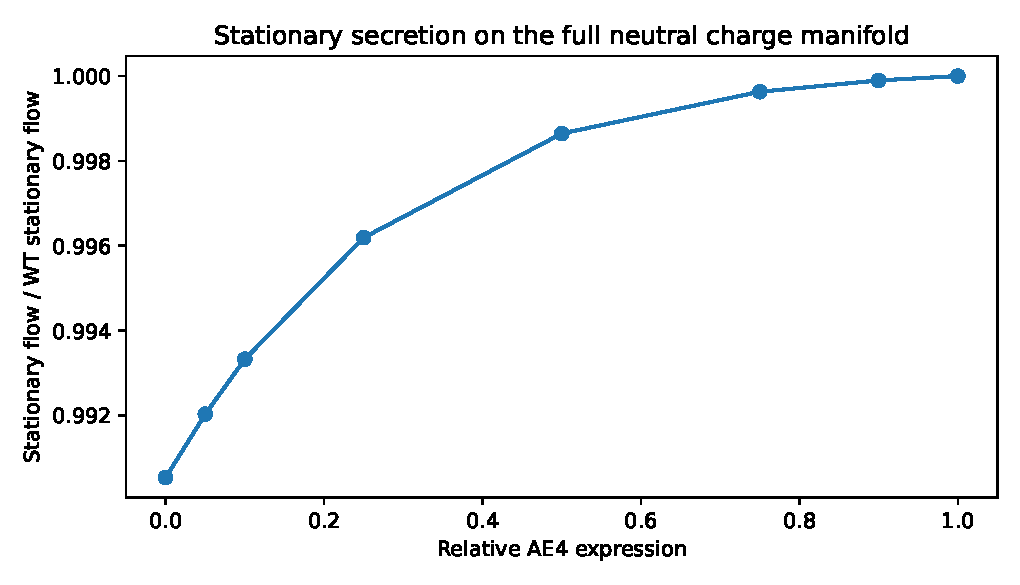
\includegraphics[width=.82\linewidth]{evidence/task44/output/equilibrium_flow.pdf}
\caption{Constant stimulus C0 equilibrium secretion normalised by WT.
The vertical axis deliberately resolves the small change around one;
the complete null deficit is 0.94617\%, not the 600 s cumulative deficit.
Each point is a solved local root, not evidence of global uniqueness.}
\end{figure}
\begin{figure}[htbp]
\centering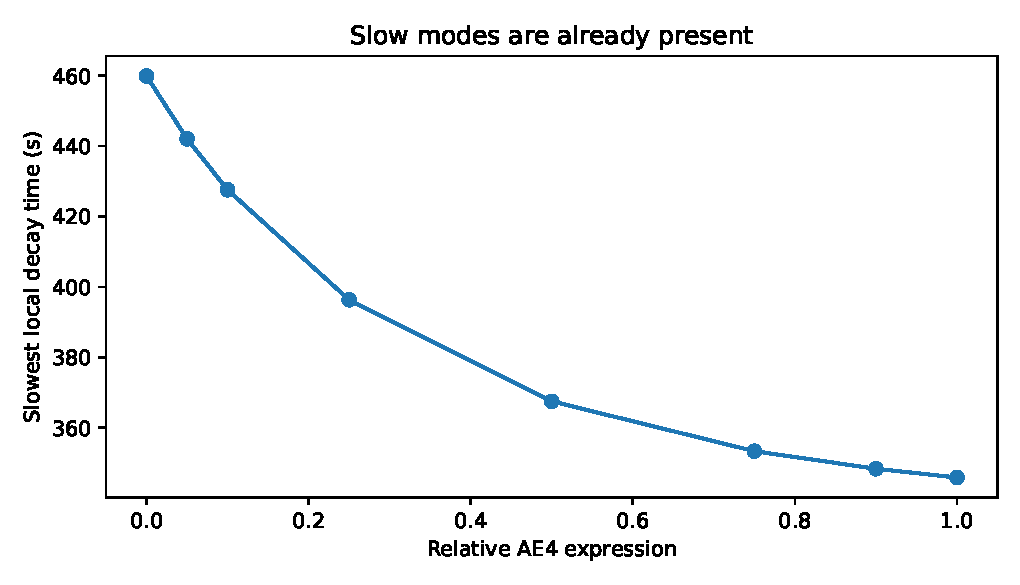
\includegraphics[width=.82\linewidth]{evidence/task44/output/slow_modes.pdf}
\caption{Dominant local decay times on the eleven dimensional neutral
manifold during expression continuation. Carbon, alkalinity, both volumes,
finite lumen composition and regulation are retained. These local
timescales do not alone establish the shape of genotype divergence.}
\end{figure}
\begin{figure}[htbp]
\centering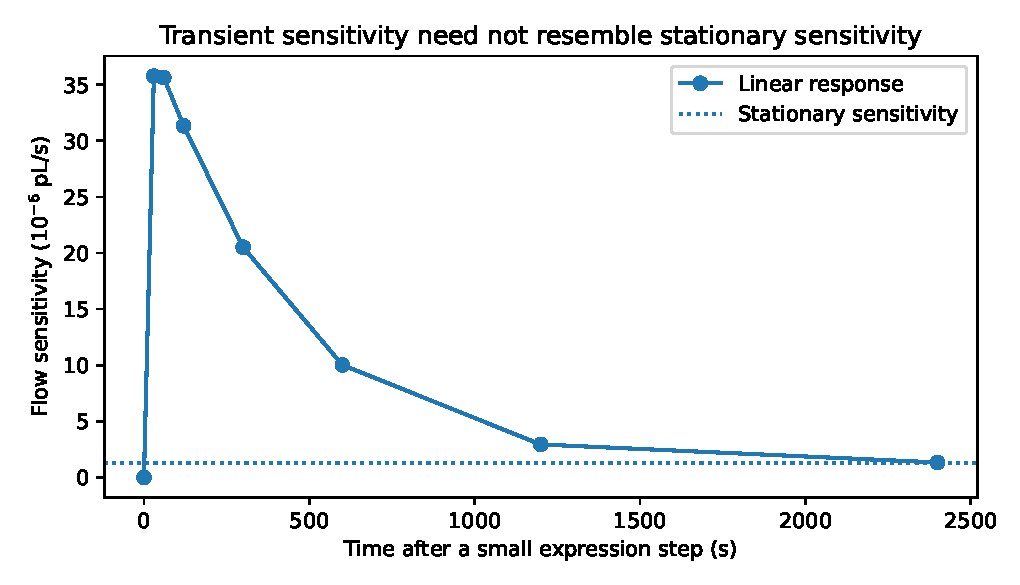
\includegraphics[width=.82\linewidth]{evidence/task44/output/linear_response.pdf}
\caption{Local expression step response at the WT equilibrium.
This linear response retains input and secretion output projection.
It is a derivative experiment, not a replacement for a finite knockout
trajectory from the inherited resting state.}
\end{figure}
\FloatBarrier

\section{All frozen source classes}
The exact projections were derived above without class specific refitting.
For completeness, the full expression root of every class is tabulated here.
Sodium concentrations are in mM. Physiological acceptance and thermodynamic
compatibility are separate tests; passing this table's gates does not erase
the opposed fluxes reported in the spectral review.
\begin{center}\small

% Expanded source: evidence/task44/output/class_table.tex
\begin{tabular}{lrrrl}
\toprule
Class & $\mathrm{pH}_i^*$ & $[\mathrm{Na}]_i^*$ & $t_{\mathrm{slow}}$ (s) & Failed criteria \\
\midrule
C0 & 7.0504 & 18.083 & 345.82 & None \\
C1 & 7.0139 & 45.694 & 564.38 & sodium \\
C2 & 6.5211 & 57.460 & 500.52 & sodium, pH \\
C3a & 7.0220 & 24.508 & 431.19 & None \\
C3b & 7.0734 & 14.206 & 314.61 & None \\
C4a & 6.5214 & 31.108 & 455.72 & pH \\
C4b & 6.5792 & 15.581 & 313.64 & pH \\
\bottomrule
\end{tabular}


\end{center}
In particular C0 is a physiological mathematical root with thermodynamic
opposition under the substituted ensemble source convention. Edge kinetics
inherited from the carrier are insufficient to guarantee consistency of
the whole substituted molecular cycle. The source vector analysis identifies
the conserved signatures that require measurement; it does not validate
the scalar kinetics for each molecular hypothesis.


% Expanded source: evidence/task44/inverse_results.tex
\section{The prescribed Task 41 inverse family}
\label{m44sec:task41inverse}

The Task 41 construction is target selected. Its added hypothesis changes
stimulated CaCC conductance before the full electrical and NBC closure:
\begin{equation}
 g_{\mathrm{CaCC}}(e,a;\rho)
 =g_{\mathrm{parent}}\{1-a\rho(1-e)\},\qquad
 \rho=1-b,\quad 0\leq\rho<1.
 \label{m44eq:inversefamily}
\end{equation}
Here $e$ is AE4 expression and $a$ is the protocol normalised recruitment
fraction used by NBC:
\[
 a=\min\!\left\{1,\max\!\left\{0,
 \frac{[\mathrm{Ca}]_i-0.058\,\mu\mathrm M}{(0.25-0.058)\,\mu\mathrm M}
 \right\}\right\}.
\]
The parent CaCC Hill gate remains a distinct retained factor.
The full conserved system, carbonate closure, electrical closure, both
volumes and AE4 regulation remain active. WT nests the parent exactly for
every state and every $\rho$. At full activation, the null retains fraction
$b=1-\rho$ of its parent CaCC conductance.

Every 600 s trajectory uses the identical frozen WT initial conserved state
and original stimulus protocol. No genotype resting solve, new mechanism or
parameter fit is introduced. All inherited positivity, concentration, pH,
volume, source and conservation gates are checked at accepted solver endpoints
and at the original observation times. The original WT stimulation requirement
is also retained; it is not imposed retrospectively on mutants.

For $X\in\{\mathrm{A},\mathrm{S}\}$ define
\begin{equation}
 D_X(\rho,p)=1-\frac{I_{0,X}(\rho,p)}{I_{1,X}(p)}.
 \label{m44eq:inverseobservable}
\end{equation}
$I_{e,\mathrm A}$ is the adaptive time integral of outflow and
$I_{e,\mathrm S}$ is the original trapezoidal observable on integer seconds,
including $t=0$ and $10^{-6}$ s. These are distinct numerical observations.
The prescribed comparison threshold is $D_X=0.303$: it is one reported
standard error below the experimental mean of 35\%, whose reported standard
error is 4.7 percentage points. It is not a confidence limit, a measured
biological range or an admissibility gate.

\subsection{Reproduction and numerical crossing}
The selected Task 41 parameter is
$b=0.10511872843288446$, or $\rho=0.8948812715671155$.
The three selected trajectories reproduce the frozen sampled cumulative
outputs to within 6.7e-10 pL.
\begin{center}
\begin{tabular}{lrrr}
\hline
Case & Sampled output (pL) & Adaptive output (pL) & Sampled deficit (\%) \\
\hline
WT & 0.992524545 & 0.992544443 & 0 \\
5\% AE4 & 0.762622459 & 0.762624862 & 23.163365 \\
AE4 null & 0.692175197 & 0.692173709 & 30.261151 \\
\hline
\end{tabular}
\end{center}
In particular, the frozen selected null deficit is slightly below 30.3\%.
It must not be described as exactly attaining this new comparison threshold.

An ordered scan of 17 recruitment fractions, followed by bracketed numerical
root refinement in the prescribed family, gives:
\begin{center}
\begin{tabular}{lrrr}
\hline
Observable & Crossing $\rho$ & AE4 dependent recruitment (\%) & Residual $b$ \\
\hline
Adaptive & 0.8950726882 & 89.5072688 & 0.1049273118 \\
Original sampled & 0.8950806285 & 89.5080628 & 0.1049193715 \\
\hline
\end{tabular}
\end{center}
Both crossings pass every inherited 600 s gate. At the adaptive crossing,
the original sampled deficit is 30.2984507\%;
at the sampled crossing, the adaptive deficit is
30.3015492\%.
Refinement at relative solver tolerances $10^{-8}$ and $2\times10^{-9}$,
with respective maximum steps 2 s and 1 s, changes the two crossing fractions
by 1.4e-13 and
1.7e-11, respectively.
Independent integration of the 13 production states, followed by adaptive
quadrature of dense flow, also reproduces the selected cases and crossing.

The deficit increases at the sampled points, but monotonicity between them
and exclusion of all earlier unsampled crossings have not been proved.
These are the first numerical crossings found in this prescribed family,
not global lower bounds, universal recruitment requirements or independent
validation of the coupling hypothesis.

\subsection{The separate extension beyond 600 s}
Continuing constant full stimulation to 3600 s gives the following null
diagnostics. Each run passes all inherited gates through 600 s. Intracellular
pH is the only later gate failure; all other monitored gates continue to pass.
\begin{center}
\begin{tabular}{lrrr}
\hline
Case & First pH $=7.3$ time (s) & pH at 3600 s & Limiting local root pH \\
\hline
Selected Task 41 & 1486.30957 & 7.3117946 & 7.3120147 \\
Adaptive crossing & 1484.74517 & 7.3118437 & 7.3120644 \\
\hline
\end{tabular}
\end{center}
The limiting roots found from these late states are mathematical continuations
outside the inherited pH domain. They do not establish globally unique
equilibria or physiological long term validity. These separate diagnostics do
not change any frozen 600 s Task 41 result.

\subsection{Local uncertainty of the crossing}
For a locally regular numerical crossing with $\partial_\rho D_X\ne0$,
\begin{equation}
 \frac{\mathrm d\rho_X}{\mathrm d\log p}
 =-\frac{\partial_{\log p}D_X}{\partial_\rho D_X},\qquad
 \frac{\mathrm d\log b_X}{\mathrm d\log p}
 =-\frac{1}{1-\rho_X}\frac{\mathrm d\rho_X}{\mathrm d\log p}.
 \label{m44eq:thresholdsensitivity}
\end{equation}
Eight effective or architecture derived quantities were selected using the
Task 43 provenance classification. A perturbed WT denominator is used with
the same perturbed parameter in the null. The conserved initial state is
always held at the inherited WT value. Thus changing the buffer amount also
changes the algebraic initial pH; it does not trigger a new resting solve.

The following elasticities refer to the adaptive crossing. The companion
sampled results are retained in the machine readable crosswalk.
\begin{center}
\begin{tabular}{lrr}
\hline
Parameter & $\mathrm d\log\rho/\mathrm d\log p$ & $\mathrm d\log b/\mathrm d\log p$ \\
\hline
NBC capacity & -0.0059550 & +0.0507982 \\
AE4 carrier amount & -0.0050569 & +0.0431371 \\
NKCC effective scale & -0.0021926 & +0.0187041 \\
NHE1 carrier amount & +0.0008018 & -0.0068396 \\
Pump capacity & -0.0355825 & +0.3035333 \\
CaCC conductance & +0.0983320 & -0.8388120 \\
Cell buffer amount & +0.0071557 & -0.0610411 \\
Apical water permeability & -0.0002975 & +0.0025380 \\
\hline
\end{tabular}
\end{center}
The derivative calculation is checked against independently solved nearby
crossings at logarithmic perturbation sizes $10^{-3}$ and $5\times10^{-4}$.
Every perturbed WT and null trajectory passes its inherited gates. The maximum
relative discrepancy between implicit crossing derivatives and nearby root
differences is 1.7e-06.
The larger relative sensitivity of residual recruitment $b$ is relevant when
interpreting a conductance assay. None of these eight quantities has an
established experimental uncertainty interval in the audited configuration.
Accordingly, these calculations establish local sensitivity only; they do
not prove robustness over a finite range or identify a finite parameter
change that overturns the conclusion.

\subsection{A discriminating experiment and scope}
At the numerical comparison crossing the null must retain approximately
10.49\% of stimulated CaCC conductance in this family. A direct test would
compare stimulated CaCC conductance and channel recruitment in WT and AE4
loss cells while matching calcium activation, voltage, intracellular chloride
and pH, so that a changed driving force is distinguished from a changed
conductance. Surface channel abundance and channel open probability would
help distinguish recruitment from gating. Concurrent measurements of pH,
chloride, cell volume and secretion over the first ten minutes and after
approximately 25 minutes would test the predicted coupled response and its
later pH failure. A secretion measurement alone does not identify this
specific dependency.


\begin{figure}[htbp]
\centering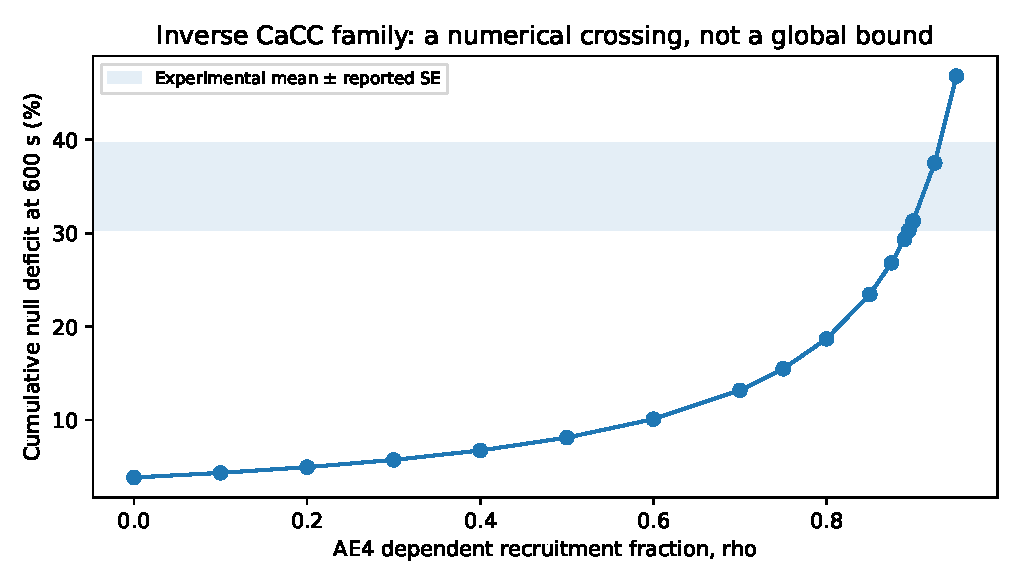
\includegraphics[width=.82\linewidth]{evidence/task44/output/inverse_threshold.pdf}
\caption{Ordered numerical scan within the one prescribed Task 41 family.
The experimental band represents the reported mean plus or minus one
standard error, not a confidence interval. The refined adaptive and sampled
crossings are recorded separately. Neither a global lower bound nor global
monotonicity follows from the plotted points.}
\end{figure}
\begin{figure}[htbp]
\centering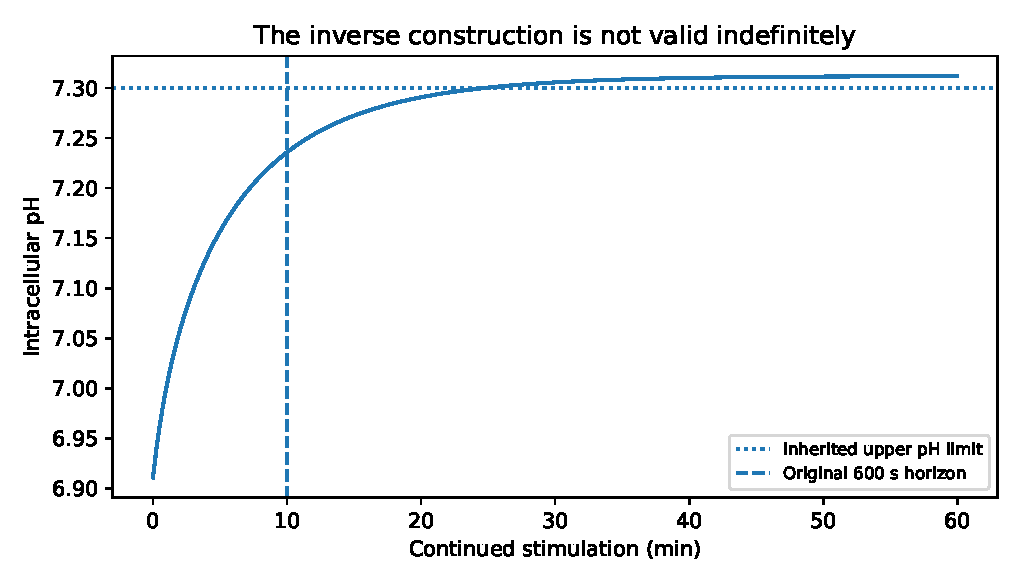
\includegraphics[width=.82\linewidth]{evidence/task44/output/inverse_ph.pdf}
\caption{Separate extension of the adaptive crossing null beyond the
declared 600 s Task 41 window. It first crosses the inherited upper pH
gate near 1485 s; the selected case has a nearly identical late crossing.
The later diagnostic does not revise the frozen 600 s
observable; it limits claims of sustained physiological validity.}
\end{figure}
\FloatBarrier

\section{Dependence on uncertain parameters}

% Expanded source: evidence/task44/sensitivity_results.tex
\subsection{Sensitivity crosswalk with Task 43}
The sixteen selected parameters are uncertain effective settings or inherited calibrated capacities. Each is perturbed independently by $p\exp(\pm h)$, with $h=10^{-3}$ and $5\times10^{-4}$; both genotypes are solved afresh at each perturbed point. These steps are numerical checks and do not define uncertainty intervals. No defensible physiological interval is available from the provenance audit, so no global robustness claim is made.
\begin{center}\small
\begin{tabular}{lrrrrr}\hline
Parameter & $E_Q$ & $\partial\mathrm{pH}/\partial\log p$ & $E_D$ & $E_{C_N}$ & $E_{\tau_{\rm WT}}$\\\hline
NBC capacity & 0.01992 & 0.06483 & 2.085 & -0.06438 & 0.107\\
AE4 amount & 0.0008114 & -0.07246 & 0.08494 & 0.02339 & -0.06397\\
NKCC scale & 0.05536 & -0.001558 & -1.494 & 0.06404 & 0.1901\\
NHE amount & -0.003261 & 0.07084 & -0.2293 & 0.007679 & -0.01473\\
Pump capacity & 0.5259 & 0.1206 & 4.634 & -0.2734 & -1.522\\
CaCC conductance & 0.03247 & -0.005524 & -0.2212 & 0.01105 & 0.008274\\
Cell buffer amount & -0.001575 & 0.001396 & -0.2063 & 0.009504 & 0.3086\\
Apical water permeability & 0.002129 & -8.317e-05 & -0.003558 & 0.0002239 & -3.74e-05\\
AE4 activation time & 0 & 0 & 0 & 0 & 0\\
AE4 activation gain & 0.0001623 & -0.01449 & 0.01699 & 0.004678 & -0.01279\\
Apical pump fraction & 0.04956 & -0.003571 & -0.05983 & 0.003151 & 0.04517\\
NHE stimulation gain & -0.003261 & 0.07084 & -0.2293 & 0.007678 & -0.01473\\
Basolateral CO$_2$ permeability & -0.004448 & -0.08319 & -0.4338 & 0.05062 & -0.06818\\
AE2 capacity & -7.335e-05 & 0.000363 & -0.03056 & -0.03383 & 7.508e-05\\
NBC saturation width & -0.01435 & -0.0467 & -1.502 & 0.01777 & -0.07263\\
NKCC stimulation gain & 0.05536 & -0.001558 & -1.494 & 0.06404 & 0.1901\\
\hline\end{tabular}\end{center}
Here $E_Y=\partial\log Y/\partial\log p$ and $D=1-Q_{\rm null}/Q_{\rm WT}$ is the stationary deficit. Its small baseline value makes $E_D$ potentially large; the machine readable table also supplies percentage point derivatives. pH is already logarithmic, so its unnormalised derivative is shown; the hydrogen concentration elasticity is $-\log(10)\partial\mathrm{pH}/\partial\log p$. All derivatives are partial sensitivities at the inherited parameter point, without recalibration.
Pump capacity has the largest local effect on WT secretion and on the stationary null deficit. The latter is also sensitive to NBC capacity and its assumed saturation width, and to effective NKCC capacity. These are priorities for experimental constraint. The calculations do not show that a finite parameter change overturns a conclusion, and cannot establish that the small null phenotype persists throughout an unknown uncertainty range. The exact balance identities survive these capacity changes within the specified architecture; their numerical consequences need not.
The equilibrium total alkalinity support ratio is identically one and cannot demonstrate robustness. The saved results instead give the NBC share $J_B/J_4$, the observed non NBC share $(J_H-J_2)/(2J_4)$, and a conditional capacity ratio $(H_{\max}+J_{2,\max})/(2J_4)$. The bound assumes the fixed bath, positive sodium and $\mathrm{pH}_i\geq6.6$. It permits AE2 to supply alkalinity at its maximal reverse capacity. Its local sensitivity is useful, but it does not prove the available capacity over an unknown parameter interval.
The AE4 activation time has no local effect on constant stimulus equilibria. Its eigenvalue is $-1/\tau_4$ and is separated from the slower chemical mode at this point; a zero local slow mode sensitivity does not establish that activation timing is irrelevant to finite time secretion. The buffer calculation holds the fixed charge and impermeant osmole pools fixed while changing only buffer amount. NKCC capacity and its stimulated multiplier produce the same stationary perturbation because only their product enters at constant full stimulation.
Independent root perturbations validate the IFT derivatives at both steps, and expression perturbations validate the chloride compensation gain at both steps for every nearby parameter point. Fixed state parameter derivatives use the smaller steps $10^{-5}$ and $5\times10^{-6}$ to resolve cancellation in the buffer response. Decay sensitivities additionally use fourth order differentiation of the chemical block at two steps, together with the exact regulatory eigenvalue; the block triangular structure retains all eleven dynamical eigenvalues. The supplied files retain root residuals, physiological gate results, Jacobian step checks and all derivative comparisons. The separate inverse family calculation supplies the Task 41 crossing sensitivity.


The independent complete gate supplement resolves all 128 perturbed WT
and null parameter roots and 256 additional expression roots used to
check compensation. Every numerical solve succeeds and every inherited
gate passes. Its largest conservation residual divided by its own tolerance
is $4.086\times10^{-5}$; the largest independent RHS residual is
$6.880\times10^{-12}$. This supplements the original derivative checks
without weakening a gate. Exact reproduction of this supplementary
calculation from the clean numerical checkout is recorded separately.


% Expanded source: evidence/task44/literature_comparison.tex
% Primary source audit, completed 15 September 2026.
% 2015: PMC4409235 full primary HTML, Experimental Procedures (Statistical
% Analyses), Results, Table 1 and Figures 1--2; retrieved with urllib after
% the web reader returned a CAPTCHA. SHA256 of retrieved HTML:
% 72dd59caaede1c477c643f818926390bf48e2966692b4dbd47b752b4f6fbe98d.
% 2018: literature/core/2018_AE4_model.pdf, pp. 258--263, 269--271;
% SHA256 e2782a89b13a6dd27ea1c510d11515bacc33931697baccb678802de47bb13a23.
% 2021: primary PubMed record 34585968, abstract and Figures 1--2 captions;
% the complete article was not required or claimed to be reread.
% 2025: PMC12463136 primary author manuscript, Methods, Results and Discussion;
% retrieved HTML SHA256:
% 890c6f4b9834e8f0c8683e181aac5c8e3d49e045d7ada3d728b1b0cc591c2583.
% No source text or protected manuscript text is copied into this section.
\section{Comparison with experimental evidence}
\label{m44sec:literature-comparison}

\paragraph{The gland phenotype and the comparison threshold.}
In the 2015 mouse submandibular gland study, stimulation used
$0.3\,\mu\mathrm{M}$ carbachol and $5\,\mu\mathrm{M}$ isoproterenol.
AE4 deletion reduced total secretion over ten minutes by
$35\pm4.7\%$ (mean $\pm$ standard error; six glands per genotype).
Initial flow over two to three minutes was comparable, with the deficit
developing later. AE2 deletion had no detectable flow effect against its
own control strain. AE4 deficient acinar cells had lower resting chloride
and slower chloride reuptake; initial chloride exit and resting pH were
not detectably changed. These are distinct measurements, rather than
interchangeable manifestations of a single steady flux~\cite{m44Pena2015}.
The prescribed $30.3\%=35\%-4.7\%$ inverse target is therefore a
comparison value one reported standard error below the mean. It is not
a confidence bound, an uncertainty interval for a model parameter, or
a universal biological minimum.

The Task 40 cumulative null deficit of $3.8575\%$ establishes a small
effect for the frozen model and protocol. The equal routing identity
does not establish that small magnitude for every admissible parameter
choice. Nor does agreement at $600\,\mathrm{s}$ establish the observed
time course. The present simulations initialise every genotype at the
inherited WT resting state, whereas the experiment used established
knockout animals. That difference should remain explicit when comparing
the initial response or stored intracellular chloride.

\paragraph{Compensation and pH.}
The 2015 isolated NKCC1 assay used bicarbonate free solution,
$30\,\mu\mathrm{M}$ ethoxyzolamide and
$50\,\mu\mathrm{M}$ T16Ainh-A01; bumetanide identified the
NKCC1 dependent component. Initial chloride uptake showed no detectable
genotype difference. Stimulation induced NHE dependent alkalinisation
also showed no genotype difference~\cite{m44Pena2015}.
Neither finding measures the complete stimulated network integral.
Consequently, the approximately $23.16\%$ rise in integrated NKCC1
loading in the frozen Task 40 null is an unresolved experimental
tension. It must not be described as observed compensation. The local
equilibrium compensation derivative, the relative integrated NKCC1
increase and the fraction of missing AE4 chloride replaced by NKCC1
are three separate quantities throughout this report. Unchanged assay
alkalinisation does not establish equal NHE1 net flux at different ionic
states, and unchanged resting pH does not identify individual alkalinity
sources. A discriminating experiment would measure chloride loading,
pH, sodium and volume through the same combined stimulus, with
pathway specific perturbations and parallel controls.

\paragraph{What the 2018 model actually established.}
The published model predicted an approximately $24\%$ flow reduction
after AE4 deletion. Its reduced flow settled within about two minutes;
the authors explicitly contrasted this with experimental development
over roughly ten minutes. It predicted little NKCC1 activation following
either exchanger deletion. It included carbon dioxide hydration, NHE1,
AE2 and AE4, without another proton or bicarbonate transporter, and
held lumen volume constant~\cite{m44VeraSiguenza2018}.
Those are historical model properties, not experimental determinations
of the full network. The present retained carbon, alkalinity and volume
coordinates make the storage terms explicit. Numerical slow modes and
their projection onto secretion must be examined before attributing a
temporal discrepancy to absent slow regulation. A slow eigenvalue alone
does not reproduce delayed genotype divergence.

\paragraph{Regulation and the inverse CaCC family.}
The 2021 study found that beta adrenergic stimulation increased native
AE4 activity, that H89 prevented the response, and that constitutively
active PKA increased AE4 activity in CHO cells. The S173A mutant lost
PKA activation, whereas S273A retained it. The authors described
phosphorylation of S173 as a probable mechanism; H89 is a nonselective
inhibitor~\cite{m44Pena2021}.
This supports regulated AE4 activity, but does not measure the model's
AE4 regulatory gain, relaxation time or an AE4 to CaCC recruitment law.
The Task 41 inverse crossing quantifies a requirement within one family
selected using the phenotype. It supplies no independent validation of
that family. Its direct experimental test is the fraction of stimulated
apical chloride conductance lost upon AE4 perturbation at matched
calcium, membrane potential, chloride, pH and volume, resolved from the
initial response into sustained secretion. This distinguishes altered
channel recruitment from changed driving force and from intracellular
chloride storage.

\paragraph{Molecular source classes.}
Catal\'an and colleagues studied human AE4 expressed in HEK293 cells,
combining mutagenesis, transport assays and molecular dynamics. The
T756A--T448I mutant lost transport with extracellular sodium while
retaining activity with potassium. Their discussion proposes both
bicarbonate and carbonate cycles, including exchanged sodium and
potassium, and explicitly calls for further experiments to resolve
the alternatives~\cite{m44Catalan2025}.
Thus the seven frozen classes are specified source hypotheses, not seven
experimentally established full cycles. Their conserved projections
and equilibrium tests separate chloride, carbon, alkalinity and charge
consequences under inherited scalar kinetics. Matching one projected
signature cannot establish identical molecular mechanisms or identical
whole cell responses. An unsuccessful root search cannot establish
nonexistence. A thermodynamically opposed or nonphysiological case must
retain that qualification. Joint measurements of cation and anion
flux ratios, reversal conditions and current would constrain the source
vector; rates measured across those gradients would constrain the
separate kinetic law.

\paragraph{The most urgent missing measurements.}
The evidence checked here does not establish the identity, abundance
or capacity of the assumed inward $1\mathrm{Na}:2\mathrm{HCO}_3$
pathway. The alkalinity proposition gives a conditional requirement for
additional support when the admissible NHE1 and AE2 contribution is
insufficient. It does not prove that a particular NBC isoform is
universally necessary. The assumed loading allocation used to construct
NBC capacity is not a measured transporter partition.
Measurements of sodium and bicarbonate influx with current and pH
during combined stimulation are therefore a priority, alongside native
NHE1 and NKCC1 capacity and state dependence. The sensitivity crosswalk
identifies which effective capacities, conductances and buffer settings
matter most at the analysed point. Until independent ranges constrain
them, local elasticities do not establish robustness over biological
uncertainty.

\paragraph{Scope of source verification.}
The comparison uses the 2015 primary full text and Figures 1 and 2,
the repository copy of the 2018 published paper, the 2021 primary
abstract and figure captions, and the 2025 primary author manuscript
including its discussion. These four references were checked to that
extent. No systematic literature survey, new experimental measurement
or complete source audit of every inherited kinetic coefficient is
claimed here; parameter provenance is recorded separately in Task 43.



\clearpage
\section{What is established and what remains unresolved}
\begin{longtable}{p{.17\linewidth}p{.76\linewidth}}
\toprule
Status & Conclusion and scope\\\midrule
\endhead
Proved or exact & Unique mathematical carbonate and electrical roots under
the stated positivity and slope assumptions, smooth dependence inside strict
executable brackets, local well posedness, exact retained nondimensionalisation,
alkalinity storage budget, conditional capacity obstruction and equal routing
chloride identity. Joint source projections have rank five.\\
Local numerical & Twenty six class/expression cases yield nonsingular stable
local roots; twenty two pass the physiological gates. WT/null slow times are
345.82/459.92 s. The stationary null deficit is 0.94617\%; the WT local
chloride compensation is 92.901\%. Local IFT and parameter derivatives
are independently verified. A physiological NBC absent equilibrium exists.\\
Finite time numerical & Frozen Task 40 observables reproduce. The 60--600 s
integrated NKCC increase is 23.163\% and missing AE4 chloride compensation
88.507\%. First numerical Task 41 crossings need about 89.51\% AE4 dependent
stimulated CaCC recruitment. The 600 s gates pass; selected continued null
cases later violate the pH gate.\\
Unresolved & Global uniqueness, stability and positivity; a justified reduced
model; global exclusion of earlier inverse crossings; robustness over unknown
parameter ranges; native carrier abundance and pathway identity; molecular
source stoichiometry and compatible kinetics; the isolated NKCC assay tension;
independent validation of the Task 41 CaCC coupling.\\\bottomrule
\end{longtable}

Several earlier interpretations require explicit correction. Stationary
cancellation does not imply zero total sensitivity or a uniformly small
phenotype. The system already contains slow chemical modes; the corrected
regulatory derivative gives 30 s, not the spurious 60 s obtained by crossing
the production clamp. The initial unsuccessful continuation record is not
evidence of nonexistence. NBC is not universally necessary for secretion
in this frozen system, though it supplies most of the larger AE4 alkalinity
demand. The old selected Task 41 point gives a sampled deficit of
30.26115\%, slightly below 30.3\%, and the refined crossing depends on
the declared integral. The comparison value is mean minus one standard
error. The construction remains target selected and its late pH failure
must accompany any claim about sustained stimulation.

The immediate experimental priorities are functional pump capacity and
apical distribution; NBC equivalent sodium/bicarbonate flux, current and
its saturation curve; ion conditioned NKCC and NHE capacity; simultaneous
TIC, buffering, pH and volume measurements; and stimulated CaCC conductance
and recruitment under acute AE4 perturbation at matched calcium and driving
forces. Source stoichiometry requires combined cation, chloride, carbon and
current measurements. These measurements would constrain the effective
parameters that dominate local sensitivities and separate a transport
pathway from a fitted phenomenological coupling. An accepted physiological
point and small numerical perturbations do not supply those missing ranges.

\section{Reproduction, verification and deliverables}
All new material is under \texttt{analysis/44\_full\_system\_mathematics/}.
The frozen scientific base is
\nolinkurl{c4d4f207f702d8eee09ab94d2d90ae90552dd641}.
The original source manifest, active parameter objects, source hashes and
recovery record distinguish scientific files from historical metadata changes.
The complete numerical checkpoint was cloned independently, checked out
detached, and regenerated with empty inverse trial caches before this
standalone report was written. All eighteen commands passed. Forty six
regenerated authoritative JSON/CSV files plus one unchanged historical
record were compared: all 331157 numeric values matched bit for bit.
Only elapsed runtime and an ancestor validated verification commit field
were excluded. All 532 inverse trial files were regenerated; the optional
cache is not part of the published scientific deliverables. All 1751 tracked
files outside Task 44 were unchanged in that clean replay.

\begin{longtable}{>{\raggedright\arraybackslash}p{.42\linewidth}>{\raggedright\arraybackslash}p{.51\linewidth}}
\toprule
File or group & Content\\\midrule\endhead
\texttt{README.md}, \texttt{RECOVERY.md} & Reproduction commands, recovered
history and derivative correction.\\
\texttt{core.py}, \texttt{run\_analysis.py} & Exact coordinates, production
adapter, scaling, continuation, local derivatives and baseline reproduction.\\
\texttt{verify\_exact.py} & Independent full RHS reconstruction, pH and
electrical closure checks, exact source and balance identities at valid states.\\
\texttt{equilibrium\_review.py} & Full physiological gates, matched
eigenvalues, modal projection and independent nearby roots.\\
\texttt{sensitivity\_analysis.py} & Sixteen uncertain parameter sensitivities
and derivative verification; Task 43 crosswalk source.\\
\texttt{verify\_sensitivity\_gates.py} & All 384 nearby roots tested against
the complete inherited gates, with solver failures retained separately.\\
\texttt{inverse\_analysis.py}, \texttt{inverse\_verify.py} & Original family,
both crossing observables, long diagnostics, eight parameter sensitivities
and independent thirteen state integration/quadrature.\\
\texttt{output/}, \texttt{inverse\_detail/} & Machine readable source audit,
scales, trajectories, roots, spectra, derivatives, projections, crossing scan,
refinement, gates and verification.\\
\nolinkurl{output/clean_recomputation_verification.json} & Exact numerical
checkpoint, commands, file comparisons, exclusions and protected file audit.\\
\texttt{report.tex}, \texttt{build.sh}, \texttt{sources.bib} & Standalone
report source, bibliography and clean build command.\\
\texttt{FINAL\_STATUS.md} & Final verified checkpoint, findings, failures,
caveats, artifact paths and checksums.\\\bottomrule
\end{longtable}

The PDF build resolves every citation and reference. Figures are generated
from saved verified results; axis ranges and the distinct observables are
stated in captions. The report, TeX fragments, vector figures and complete
machine readable outputs are retained for scientific review. No model
source, frozen output, Task 1--42 analysis or manuscript text was changed.
The two analysis branches remain separate and unmerged.


\clearpage
\part{Complete parameter provenance from the final Task 43 sources}
The following chapters retain the completed Task 43 audit and its complete inventory table. The additional parameter records in Part IV expose the detailed justification fields that were only supplied electronically in that source report. The original source bibliography is preserved separately; duplicate reference keys in this combined document are namespaced rather than silently reconciled.
\sourcefile{evidence/task43/report.tex; evidence/task43/output/parameter_inventory.json}
\newcommand{\InventoryCount}{137}
\newcommand{\ActiveCount}{109}
\newcommand{\SensitivitySourceCommit}{f783785a863440df459e9c5530beba4c7eb59110}

\section{Source of the audit}
The audit uses repository \url{https://github.com/esig626/ae4-salivary-transport-control} at main revision \texttt{c4d4f207f702d8eee09ab94d2d90ae90552dd641}. It loads the actual nested Task 40 model through its historical validation helper and checks the complete active parameter hashes against \path{results/40_ae4_equal_cation_routing/frozen_inputs.json}. It does not overwrite the helper or weaken its historical numerical checks. The canonical initial condition is the separately frozen WT resting state, not the constructor default tuple.

The model lineage includes the original AE4 reconstruction \citep{p43VeraSiguenza2018}, the Palk and Benjamin NKCC1 law \citep{p43Palk2010,p43Benjamin1997}, and the Cha NHE kinetic model \citep{p43Cha2009}. The experimental evidence for AE4 transport and regulation constrains mechanism and direction, but does not automatically identify every abundance, gain or timescale in this implementation \citep{p43Pena2015,p43Pena2016,p43Pena2021,p43Catalan2025}. This report preserves that distinction.

\section{What counts as a justification}
A published numerical coefficient has a source, but transfer from another tissue or model still needs an applicability argument. A value determined by a balance equation is justified conditional on the concentrations, fluxes and structural assumptions used in that balance. A value selected to keep a reference trajectory within physiological limits is an effective modelling choice; acceptance of that trajectory does not make the value measured, unique, or known within an uncertainty interval. A numerical inversion bracket is not a physiological observation. A parameter selected using the knockout phenotype must remain labelled as an inverse design choice.

The inventory records value, units, original metadata, active role, classification, exact code locations, the equation role and source, mathematical justification, default value and whether the active value differs from that default. Separate fields state what constrains each quantity, what does not justify it, its logical domain, its uncertainty status, its relevance to manuscript conclusions, and an experiment that could constrain it. Classification is conservative: inherited metadata identifies a lineage, not a newly verified measurement of salivary transporter abundance. Each physiological uncertainty interval remains explicitly null in the machine readable inventory. Logical positivity or fractional bounds are not substituted for experimental uncertainty.

The current categories include physical constants; published kinetic coefficients; inherited model conversions or settings; reference and WT constraint derived values; WT architecture derived values; effective assumptions; numerical brackets and regularisation; protocol and law selections; inactive legacy values; constructor seeds; and the target selected Task 41 parameter. These categories should not be collapsed into a single ``from the literature'' column.

\section{Parameters that can be explained mathematically}
\subsection{NKCC1 scale: derived from a modelled resting flux}
The production law has the form
\[
 J_N=\alpha_Nm_N(t)\psi([Na]_i,[K]_i,[Cl]_i),\qquad
 \psi=\frac{A_1-A_2[Na]_i[K]_i[Cl]_i^2}
 {A_3+A_4[Na]_i[K]_i[Cl]_i^2}.
\]
At the accepted resting state, the scale is determined by
\begin{equation}
 \alpha_N=\frac{J_{N,rest}}{\psi(c_{rest})}
 =0.017334746894096052\ \mathrm{fmol/s}.
 \label{p43eq:nkcc-scale}
\end{equation}
Equation \cref{p43eq:nkcc-scale} makes the choice reproducible and avoids an independent extra fit. However, $J_{N,rest}$ is itself an inherited model flux. The scale is not a directly measured salivary carrier amount. The much larger legacy field \path{homeostasis.nkcc1_capacity_fmol_s} is inactive for this selected law and must not appear in a publication table as its active capacity.

The four Palk coefficients contain fourth order concentration factors. Their conversion to mM is essential. They are effective coefficients for the adopted fixed bath, so an uncertainty study that changes bath composition cannot automatically reuse them without rechecking the underlying reduction.

\subsection{NHE1 carrier amount: a WT resting pH calibration}
The active NHE1 law is the eight state Cha reduction with its Mod2 term. Printed rate and binding constants are retained, including the documented rounding discrepancy in the fourth reverse rate. The salivary carrier amount is
\[
 N_H=2.339370005697548\times10^{-5}\ \mathrm{fmol}.
\]
This was determined against a resting pH target of 6.91 on the selected R09 background. The derivation fixes one scale conditional on that background and target. It does not identify a cardiac carrier count as a salivary measurement, nor does it prove unique joint identification of the carrier amount, buffer pool and other pH pathways.

The completion audit also records the fixed Mod2 exponents $n_H=3$ and $m_H=1$, which were absent from the earlier inventory because they are module constants rather than dataclass fields. Both are part of the selected kinetic law. Their inclusion corrects an inventory omission without changing the model.

Legacy tanh NHE capacity and older NHE kinetic fields remain in the dataclass for other models, but are inactive in production. The active stimulus multiplier is 2.3. Calling it fixed before the test documents absence of retuning; it does not establish that its transfer to every tissue and stimulus is exact. The mathematical companion report shows explicitly how the alkalinity bound depends on this multiplier and $N_H$.

\subsection{NBC capacity: derived conditional on an assumed partition}
The NBC source imports one sodium and two bicarbonate equivalents per inward cycle. Its capacity is
\[
 G_B=0.11570913197464398\ \mathrm{fmol/s}.
\]
The construction begins from the assumed fraction $s=0.70$ of positive WT chloride loading assigned to NKCC1 at the Task 31 reference scale. If that NKCC1 chloride flux is $L_N$, the corresponding AE4 demand is
\begin{equation}
 J_{4,req}=\frac{1-s}{s}L_N.
 \label{p43eq:partition}
\end{equation}
Using $L_N=0.2562444047732706$ fmol/s and the selected stimulated NHE flux, the approximate reference requirement is $B_{req}=J_{4,req}-H_{stim}/2$, before evaluating the full coupled electrical closure. The capacity is then chosen so the NBC law supplies that cycle rate at the reference chemical state with its self consistent voltage. The derivation is recorded in the unchanged Task 36 design and NBC module.

This is a conditional structural construction, not a knockout fit and not a measured transporter density. In particular, \cref{p43eq:partition} does not turn the 70/30 partition into experimental evidence. The subsequently evolved trajectory need not retain that partition exactly. The manuscript should state the assumed partition, how it sets the capacity, and what changes when that assumption changes. A broad uncertainty interval for $s$ has not been established by this audit.

The NBC increment is zero at the declared resting calcium and fully recruited at $0.25\ \mu$M. Its width parameter is effective. Its molecular identity is deliberately not assigned to a particular salivary SLC4 isoform.

\subsection{Fixed charge and osmotic pools}
Reference electroneutrality determines the fixed intracellular anion equivalent amount from
\[
 X=n_{Na,i}+n_{K,i}-n_{Cl,i}-n_{A,i}.
\]
The active value is $78.06176220594485$ fmol equivalents. Its status is reference constraint derived, conditional on the reference tuple and carbonate buffer model. It is not a directly counted molecular pool.

The other impermeant osmotic pool is $124.69936937124379$ fmol on the selected background, rather than the smaller dataclass default. It is an inherited effective osmotic setting. The separate finite intracellular buffer amount is 30 fmol and is counted exactly once in the osmolarity. Effective osmotic closure and charge closure are different roles and should not be conflated.

\section{Parameters that remain assumptions or transferred settings}
The AE4 carrier amount and transition attempt rates are inherited effective model settings. Their thermodynamic construction constrains rate ratios and reversal properties of the parent cycle; it does not supply independent measurements of the absolute carrier number or all attempt rates. Moreover, fixed source substitution in the later mechanism panel does not itself establish thermodynamic consistency of the inherited scalar kinetics with each substituted cycle.

Channel conductances, pump capacity and apical fractions determine current closure and the distribution of secretion. Their active values are explicit in the inventory, but physiological feasibility at one reference point is not evidence that each value is unique. The same applies to the effective outlet rate and dead volume. The code itself describes the outlet law as a transparent compliance closure rather than a calibrated secretion law.

The water coefficients are inherited model conversions with stated units. They should be described as transferred model parameters, not newly measured hydraulic permeabilities of the present preparation. The effective beta activation time of 30 s and AE4 gain of 0.25 likewise need to remain explicit assumptions. Experimental activation of a pathway does not identify all intermediate time constants \citep{p43Pena2021}.

The NKCC1 algebraic recruitment reaches its endpoint at $0.10\ \mu$M calcium, while NBC reaches its endpoint at $0.25\ \mu$M. The production input fully recruits both. This difference is preserved and recorded, not silently reconciled. Any analysis of submaximal calcium would need to account for it.

The numerical pH bracket from 3 to 11 only enables inversion; the actual inherited physiological criterion is pH 6.6 to 7.3. The tiny positive luminal buffer amount $10^{-9}$ fmol is numerical regularisation approximating no fixed luminal buffer, not an abundance measurement. Constructor concentrations and volumes do not replace the frozen solved initial state used by the production experiments.

Finally, the Task 41 residual CaCC recruitment coefficient $b=0.10511872843288446$ is target selected. It is not an active parameter of the parent Task 40 model and is not reclassified as literature supported merely because the resulting trajectory has an appropriate secretion magnitude.

The CCh and IPR dose fields, $0.3$ and $5\ \mu$M respectively, are experiment labels in this implementation. The selected input callable returns prescribed calcium and beta activation from the input arm and time window; it does not map those dose values through a dose response law. They are therefore retained as protocol metadata but marked inactive for the selected right hand side. The previous inventory incorrectly marked both active. Changing the nominal dose labels alone cannot change the model trajectory.

The frozen initial state is now recorded separately, with all twelve conserved amount and volume coordinates and the AE4 regulatory fraction. The twelve constructor reference fields remain distinct. The upstream NBC design quantities, selected transport laws, R1 regulatory family and WT construct are also explicit. These additions explain the larger record count; they add no fitted degrees of freedom.

The externally passed WT genotype object and the three prescribed AE4 expression values, $1$, $0.05$ and $0$, are also recorded. The other transporter expression multipliers remain one in those comparisons. These values define interventions, not an uncertainty interval for protein abundance. The prescribed Task 41 family requires $0<b\leq1$, equivalently $0\leq\rho<1$; the endpoint $b=0$ is outside its implemented domain.

The additional file \path{output/numerical_controls.json} records the production integration specification, conservation tolerances, pH inversion tolerances and voltage bracket. In particular, $[-0.5,0.5]$ V is the implemented voltage search bracket and not a measured physiological voltage interval. Integration begins at $10^{-6}$ s with the shared frozen state; the distinct resting observable at exactly $t=0$ is preserved. Exact unit conversions are stated separately from physiological settings.

\section{What the mathematical analysis adds to justification}
The separate Task 44 report uses the unchanged reference parameter set and retains carbon, alkalinity, volume, lumen and electrical feedback. It supplies exact structural identities and a conditional NHE supply bound, then evaluates local stationary sensitivities. These calculations help identify which assumptions affect which conclusions. They do not estimate experimental uncertainty intervals.

An important distinction is between statements independent of capacities, such as the cancellation of the explicit equal routing AE4 term in the chloride balance, and numerical conclusions that depend on the adopted kinetics and scales, such as large NKCC1 replacement. Even an exact balance identity does not determine the magnitude of the knockout flow deficit. The dependence of pump and NHE fluxes on state remains part of the mechanism.

For later manuscript development, every nonliterature value should therefore be accompanied by either its conditional derivation or a plainly stated effective role. Where several values were selected together on the same WT background, their correlation should be retained in future uncertainty work. Independently perturbing every value as though each had its own measured error bar would create an unsupported uncertainty model.

The remaining parameter work is substantive rather than typographical: independently justify or measure ranges for the effective settings; define a WT feasible set using evidence not reused from the knockout comparison; and assess which conclusions survive across that set. A local derivative or a collection of physiologically passing simulations does not prove robustness over all plausible parameterisations. This audit has performed no new fitting and established no calibrated uncertainty intervals.

\subsection{Completed sensitivity crosswalk}
The completed companion calculation examines sixteen uncertain or effective settings. All 128 nearby WT and AE4 null equilibrium solves pass the inherited physiological gates. Parameter differences of $10^{-3}$ and $5\times10^{-4}$ in log coordinates are numerical verification steps, not uncertainty ranges. The machine readable crosswalk reads the verified results directly from immutable Task 44 numerical source commit \texttt{\SensitivitySourceCommit} and records SHA256 hashes of all seven imported source files. Later report-only commits need not have that same head SHA. It maps every companion parameter name back to the actual inventory value and classification.

At the adopted constant full stimulus equilibrium, WT secretion is $0.0015840671$ pL/s and intracellular pH is $7.0503863$. The AE4 null stationary secretion deficit is $0.94617\%$. This stationary deficit is distinct from the frozen Task 40 cumulative deficit of $3.8575\%$ at 600 s. Intracellular storage, changing volumes, finite lumen composition and regulation remain active in the companion analysis.

In the table, $E_Q=d\log Q_{WT}/d\log p$, $E_D=d\log D/d\log p$ for the positive stationary null deficit $D$, and $E_{\tau}=d\log\tau_{slow,WT}/d\log p$. The pH column uses $d\mathrm{pH}/d\log p$ because pH is already logarithmic. A large elasticity of a small deficit is not a large absolute percentage point change.

% Expanded source: evidence/task43/output/sensitivity_table.tex
\begin{table}[tbp]
\centering\small
\begin{tabular}{p{.36\textwidth}rrrr}
\toprule Setting & $E_Q$ & $d\mathrm{pH}/d\log p$ & $E_D$ & $E_{\tau}$ \\ \midrule
NBC capacity & 0.019923 & 0.064832 & 2.0848 & 0.10701 \\
AE4 carrier & 0.00081137 & -0.072461 & 0.084942 & -0.063968 \\
NKCC scale & 0.055361 & -0.001558 & -1.4937 & 0.19015 \\
NHE carrier & -0.0032611 & 0.070838 & -0.22928 & -0.014728 \\
pump capacity & 0.52593 & 0.12061 & 4.6337 & -1.5222 \\
CaCC conductance & 0.03247 & -0.0055239 & -0.22116 & 0.0082736 \\
buffer pool & -0.0015749 & 0.0013957 & -0.20631 & 0.30856 \\
water apical & 0.0021295 & -8.3167e-05 & -0.003558 & -3.7398e-05 \\
AE4 tau & 0 & 0 & 0 & 0 \\
AE4 gain & 0.00016227 & -0.014492 & 0.016988 & -0.012794 \\
apical pump fraction & 0.049564 & -0.0035713 & -0.059826 & 0.045169 \\
NHE stimulated multiplier & -0.0032611 & 0.070838 & -0.22928 & -0.014728 \\
CO2 basolateral permeability & -0.004448 & -0.083186 & -0.43378 & -0.068179 \\
AE2 capacity & -7.3346e-05 & 0.00036297 & -0.030565 & 7.5082e-05 \\
NBC log width & -0.014352 & -0.046703 & -1.5016 & -0.072634 \\
NKCC stimulated multiplier & 0.055361 & -0.001558 & -1.4937 & 0.19015 \\
\bottomrule\end{tabular}
\caption{Local stationary sensitivities imported from Task 44. No measured uncertainty intervals are implied.}
\end{table}



The largest local sensitivities of the stationary null deficit are to pump capacity ($E_D=4.634$), NBC capacity ($2.085$), NBC saturation width ($-1.502$), and NKCC effective capacity ($-1.494$). These values identify priorities for experimental constraint. They do not establish a finite parameter change that recovers the experimental phenotype. The common stationary effects of NHE carrier amount and its stimulated multiplier reflect their product under full stimulation; separate resting and stimulated measurements are needed to distinguish them.

At the WT equilibrium, NBC supplies $95.48\%$ of the AE4 alkalinity demand. Under the stated bath composition and inherited intracellular pH lower gate of 6.6, the conditional NHE/AE2 capacity calculation covers at most $57.96\%$ of that current demand without NBC. This comparison holds the required AE4 demand at the analysed level; it does not rule out a lower supported flux, another admissible state or an additional pathway. The capacity ratio has local elasticity $0.931$ to NHE carrier amount and to the stimulated NHE multiplier. Direct measurements of maximal acid extrusion are therefore essential before treating the conditional obstruction as a biological conclusion.

The companion continuation also finds a physiological equilibrium with zero NBC capacity: pH $6.96833$ and secretion $0.00153598$ pL/s, only $3.035\%$ below the full NBC equilibrium. Its AE4 cycle flux falls from $0.0750724$ to $0.00632651$ fmol/s. Consequently, any earlier broad claim that NBC is structurally necessary for secretion must be qualified: the proved obstruction concerns sustaining the specified AE4 loading level. It does not imply that all physiological secretion fails without NBC.

The WT and null slowest local decay times are approximately $346$ and $460$ s. The WT decay time is particularly sensitive to pump capacity ($E_{\tau}=-1.522$) and the finite intracellular buffer pool ($0.309$). The model therefore already contains slow modes. The effective AE4 regulatory time has zero local stationary influence in the selected R1 family while the slower chemical mode remains dominant; this is not evidence that time dependent regulation is irrelevant. Acute pH, TIC and volume measurements alongside secretion would constrain those chemical modes and their observable effects.

The separate inverse calculation stays inside the one prescribed Task 41 family. Its first numerical 600 s crossing requires an AE4 dependent stimulated CaCC fraction $\rho\simeq0.89507$, approximately $89.51\%$. The original selected value $\rho=1-b=0.89488127$ gives the frozen $30.2612\%$ deficit, slightly below the exact $30.3\%$ comparison threshold. The threshold is $35\%$ minus the reported standard error of $4.7$ percentage points in the 2015 comparison; it is not a confidence bound. Adaptive integration and the original sampled trapezoidal observable are retained separately in the companion files. This is the first crossing found in the ordered numerical scan. Monotonicity between samples and exclusion of earlier unsampled crossings are unproved; it is neither a global lower bound nor a universal recruitment requirement.

Inverse sensitivities hold the inherited conserved WT initial state fixed, perturb the WT denominator and null system together, and perform no new resting solve. A buffer perturbation therefore changes the initial algebraic pH. Within that family, the adaptive crossing has local log elasticity $0.09833$ to CaCC conductance and $-0.03558$ to pump capacity, larger in magnitude than its elasticities to the other six tested settings. The relative sensitivity of the residual independent recruitment $1-\rho$ is also recorded, because a small change in $\rho$ can be a larger relative change in the remaining approximately $10.49\%$. Under continued full stimulation, both the selected and crossing null cases eventually violate the inherited upper pH gate at about $1485$~s. This diagnostic does not change their declared 600 s results, but prevents an unsupported long duration interpretation.

The most urgent experiments consequently differ by claim. Functional pump turnover and membrane distribution, NBC capacity and saturation shape, and ion conditioned NKCC uptake constrain secretion and compensation. Maximal NHE acid extrusion constrains the conditional alkalinity obstruction. Buffer titration with TIC and volume time series constrains slow relaxation. Matched CaCC current measurements during acute AE4 perturbation would directly test the very large recruitment dependence required by the inverse family. Strong modelled NKCC compensation remains in tension with the isolated 2015 NKCC assay; changing the assay context in the model does not erase that discrepancy.

\section{Reproducibility and use in the manuscript}
Run \texttt{python analysis/43\_parameter\_provenance/audit.py} from the repository root. It verifies the production parameter hashes and writes both CSV and JSON inventories under this task's \texttt{output} directory. Each record contains source paths and justification notes beyond the abbreviated table below. \texttt{prepare\_report.py} typesets the table from those records. The report and the full inventory belong on the Task 43 branch, separate from the mathematical analysis and from the main manuscript.

The inventory has \InventoryCount{} records and \ActiveCount{} active flags. This is an inventory of configuration and roles, not a count of independent degrees of freedom: it includes physical constants, protocol settings, law selections, derived values and other nonfit quantities. Five legacy fields and twelve constructor seed fields are explicitly separated. The Task 41 inverse coefficient is also outside the parent model.

Run \path{analysis/43_parameter_provenance/verify.py} to compare the saved CSV/JSON products with a fresh reconstruction, check every nested production field, verify source hashes, confirm the fixed Cha exponents and demonstrate that changing dose labels leaves the selected input unchanged. The audit performs no fresh sensitivity simulations. With the companion commit available in the fetched Git history, \path{import_crosswalk.py --check} independently reconstructs the saved crosswalk from that exact commit; no adjacent Task 44 working directory is required. The report tables are also checked against their machine readable sources. The source manifest contains SHA256 values for the production modules and frozen inputs; verification also checks that protected paths are unchanged from recovered Task 43 checkpoint \texttt{693f44c0b05e92faec737aa7793c3a99ec76445c}.

No model source, historical analysis, frozen trajectory or main manuscript is modified by this audit. The exact original metadata is retained in the machine readable inventory, while the new classification states what that metadata does and does not justify.

% Appendix integrated in combined section sequence
\section{Complete active object and legacy inventory}
The ``Used'' column denotes use by the selected production configuration as classified by the audit. ``No'' for constructor seeds means they are not the production initial state; the constructor still uses that tuple for reference consistency checks. Full units, source locations, defaults and detailed justifications are in \texttt{parameter\_inventory.csv} and \texttt{parameter\_inventory.json}.

% Expanded source: evidence/task43/output/inventory_table.tex
\setlength{\tabcolsep}{4pt}
\small
\begin{longtable}{p{.38\textwidth}p{.17\textwidth}p{.11\textwidth}p{.25\textwidth}}
\toprule Setting & Value & Used & Classification \\ \midrule\endfirsthead
\toprule Setting & Value & Used & Classification \\ \midrule\endhead
\bottomrule\endfoot
\path{constants.temperature_K} & 310.15 & Yes & effective assumption \\
\path{constants.gas_constant_J_mol_K} & 8.31446262 & Yes & physical constant \\
\path{constants.faraday_C_mol} & 96485.3321 & Yes & physical constant \\
\path{acid_base.carbon_pka1} & 6.1 & Yes & inherited model setting \\
\path{acid_base.carbon_pka2} & 10.3 & Yes & inherited model setting \\
\path{acid_base.water_pkw} & 14 & Yes & inherited model setting \\
\path{acid_base.cell_buffer_pka} & 7 & Yes & effective assumption \\
\path{acid_base.lumen_buffer_pka} & 7 & Yes & effective assumption \\
\path{acid_base.ph_lower} & 3 & Yes & numerical bracket \\
\path{acid_base.ph_upper} & 11 & Yes & numerical bracket \\
\path{bath.na_mM} & 145 & Yes & effective assumption \\
\path{bath.k_mM} & 5 & Yes & effective assumption \\
\path{bath.cl_mM} & 126.161593 & Yes & reference constraint derived \\
\path{bath.tic_mM} & 25 & Yes & effective assumption \\
\path{bath.ph} & 7.4 & Yes & effective assumption \\
\path{bath.buffer_total_mM} & 0 & Yes & effective assumption \\
\path{bath.untracked_osmolyte_mM} & 0 & Yes & effective assumption \\
\path{geometry.cell_buffer_total_fmol} & 30 & Yes & effective assumption \\
\path{geometry.lumen_buffer_total_fmol} & 1e-09 & Yes & numerical regularisation \\
\path{geometry.fixed_cell_anion_equivalents_fmol} & 78.0617622 & Yes & reference constraint derived \\
\path{geometry.cell_impermeant_osmoles_fmol} & 124.699369 & Yes & inherited effective setting \\
\path{homeostasis.nkcc1_capacity_fmol_s} & 0.32 & No & inactive legacy \\
\path{homeostasis.nhe1_capacity_fmol_s} & 0.00744098059 & No & inactive legacy \\
\path{homeostasis.nhe1_model} & \path{cha_2009_eight_state_mod2} & Yes & law selection \\
\path{homeostasis.nhe1_published_g_fmol_s} & 0.0305 & No & inactive legacy \\
\path{homeostasis.nhe1_published_k_h_mM} & 0.00045 & No & inactive legacy \\
\path{homeostasis.nhe1_published_k_na_mM} & 15 & No & inactive legacy \\
\path{homeostasis.nhe1_cha_carrier_amount_fmol} & 2.33937001e-05 & Yes & WT constraint derived \\
\path{homeostasis.ae2_capacity_fmol_s} & 0.005 & Yes & effective assumption \\
\path{homeostasis.thermodynamic_saturation_log_width} & 2 & Yes & effective assumption \\
\path{homeostasis.co2_basolateral_permeability_fmol_s_mM} & 0.02 & Yes & effective assumption \\
\path{homeostasis.co2_apical_permeability_fmol_s_mM} & 0.01 & Yes & effective assumption \\
\path{membranes.nak_capacity_fmol_s} & 0.08 & Yes & effective assumption \\
\path{membranes.nak_na_half_mM} & 10 & Yes & inherited model setting \\
\path{membranes.nak_k_half_mM} & 1.5 & Yes & inherited model setting \\
\path{membranes.apical_pump_fraction} & 0.075075 & Yes & effective assumption \\
\path{membranes.apical_k_fraction} & 0.3 & Yes & effective assumption \\
\path{membranes.g_k_total_S} & 1.4e-08 & Yes & effective assumption \\
\path{membranes.g_cl_apical_S} & 3.14e-08 & Yes & effective assumption \\
\path{membranes.calcium_half_uM} & 0.26 & Yes & effective assumption \\
\path{membranes.calcium_hill} & 1.46 & Yes & effective assumption \\
\path{membranes.g_para_na_S} & 3e-10 & Yes & inherited model setting \\
\path{membranes.g_para_k_S} & 5e-11 & Yes & inherited model setting \\
\path{membranes.g_para_cl_S} & 2.5e-10 & Yes & effective assumption \\
\path{membranes.g_para_hco3_S} & 5e-11 & Yes & effective assumption \\
\path{membranes.g_apical_background_S} & 0 & Yes & effective assumption \\
\path{membranes.g_basolateral_background_S} & 0 & Yes & effective assumption \\
\path{water.apical_hydraulic_pL_s_mOsm} & 0.00432 & Yes & published model conversion \\
\path{water.basolateral_hydraulic_pL_s_mOsm} & 0.0515 & Yes & published model conversion \\
\path{water.paracellular_hydraulic_pL_s_mOsm} & 0.00026 & Yes & published model conversion \\
\path{water.lumen_dead_volume_pL} & 0.1 & Yes & effective assumption \\
\path{water.outflow_rate_s} & 0.2 & Yes & effective assumption \\
\path{initial.cell_na_mM} & 15 & No & constructor seed \\
\path{initial.cell_k_mM} & 140 & No & constructor seed \\
\path{initial.cell_cl_mM} & 40 & No & constructor seed \\
\path{initial.cell_tic_mM} & 20 & No & constructor seed \\
\path{initial.cell_ph} & 7.2 & No & constructor seed \\
\path{initial.cell_volume_pL} & 1 & No & constructor seed \\
\path{initial.lumen_na_mM} & 145 & No & constructor seed \\
\path{initial.lumen_k_mM} & 5 & No & constructor seed \\
\path{initial.lumen_cl_mM} & 126.161593 & No & constructor seed \\
\path{initial.lumen_tic_mM} & 25 & No & constructor seed \\
\path{initial.lumen_ph} & 7.4 & No & constructor seed \\
\path{initial.lumen_volume_pL} & 0.1 & No & constructor seed \\
\path{ae4.carrier_amount_fmol} & 0.150126427 & Yes & inherited effective setting \\
\path{ae4.common_cl_attempt_rate_s} & 1 & Yes & inherited effective setting \\
\path{ae4.na_loaded_attempt_rate_s} & 0.1 & Yes & inherited effective setting \\
\path{ae4.k_loaded_attempt_rate_s} & 1.9 & Yes & inherited effective setting \\
\path{ae4.cooperative_gate} & \path{None} & No & inherited effective setting \\
\path{nbc.capacity_fmol_s} & 0.115709132 & Yes & WT architecture derived \\
\path{nbc.log_width} & 2 & Yes & effective assumption \\
\path{nbc.resting_calcium_uM} & 0.058 & Yes & effective assumption \\
\path{nbc.fully_recruited_calcium_uM} & 0.25 & Yes & effective assumption \\
\path{nbc.nhe1_stimulated_multiplier} & 2.3 & Yes & effective assumption \\
\path{nkcc.alpha_eff_fmol_s} & 0.0173347469 & Yes & WT constraint derived \\
\path{nkcc.A1} & 157.5 & Yes & published kinetic coefficient \\
\path{nkcc.A2} & 2.0096e-05 & Yes & published kinetic coefficient \\
\path{nkcc.A3} & 1.0306 & Yes & published kinetic coefficient \\
\path{nkcc.A4} & 1.3852e-06 & Yes & published kinetic coefficient \\
\path{cha.k1_plus_per_ms} & 10.5 & Yes & published kinetic coefficient \\
\path{cha.k1_minus_per_ms} & 0.201 & Yes & published kinetic coefficient \\
\path{cha.k2_plus_per_ms} & 15.8 & Yes & published kinetic coefficient \\
\path{cha.k_na_o_mM} & 195 & Yes & published kinetic coefficient \\
\path{cha.k_na_i_mM} & 16.2 & Yes & published kinetic coefficient \\
\path{cha.k_h_o_mM} & 0.00162 & Yes & published kinetic coefficient \\
\path{cha.k_h_i_mM} & 0.000605 & Yes & published kinetic coefficient \\
\path{cha.modifier_k_i_mM} & 3.07e-05 & Yes & published kinetic coefficient \\
\path{cha.modifier_k_o_mM} & 4.8e-07 & Yes & published kinetic coefficient \\
\path{cha.k2_minus_table_per_ms} & 183 & Yes & published kinetic coefficient \\
\path{regulation.tau_ae4_s} & 30 & Yes & effective assumption \\
\path{regulation.basal_capacity_multiplier} & 1 & Yes & effective assumption \\
\path{regulation.fully_activated_increment} & 0.25 & Yes & effective assumption \\
\path{regulation.coupling_scale} & 1 & Yes & effective assumption \\
\path{nkcc_activation.fully_activated_multiplier} & 1.75 & Yes & inherited effective setting \\
\path{nkcc_activation.resting_calcium_uM} & 0.058 & Yes & inherited effective setting \\
\path{nkcc_activation.stimulated_calcium_uM} & 0.1 & Yes & inherited effective setting \\
\path{protocol.arm} & \path{CCH_IPR} & Yes & protocol setting \\
\path{protocol.onset_s} & 0 & Yes & protocol setting \\
\path{protocol.duration_s} & 600 & Yes & protocol setting \\
\path{protocol.cch_dose_uM} & 0.3 & No & protocol setting \\
\path{protocol.ipr_dose_uM} & 5 & No & protocol setting \\
\path{protocol.resting_calcium_uM} & 0.058 & Yes & protocol setting \\
\path{protocol.stimulated_calcium_uM} & 0.25 & Yes & protocol setting \\
\path{protocol.beta_occupancy_on} & 1 & Yes & protocol setting \\
\path{Task41.b} & 0.105118728 & No & target selected \\
\path{cha.intracellular_modifier_hill} & 3 & Yes & published kinetic coefficient \\
\path{cha.extracellular_modifier_hill} & 1 & Yes & published kinetic coefficient \\
\path{nkcc.law} & \path{palk_benjamin_2010_eq17} & Yes & law selection \\
\path{ae4.law} & \path{equal_routing_adapter} & Yes & law selection \\
\path{regulation.family} & \path{R1} & Yes & law selection \\
\path{regulation.construct} & \path{WT} & Yes & protocol setting \\
\path{nkcc_activation.family} & \path{N1_CCH_ALGEBRAIC} & Yes & law selection \\
\path{nbc_design.TARGET_NKCC1_POSITIVE_CL_SHARE} & 0.7 & No & effective assumption \\
\path{nbc_design.TASK31_R09_NKCC1_CL_FMOL_S} & 0.256244405 & No & WT architecture derived \\
\path{nbc_design.TASK31_R09_NHE1_FMOL_S} & 0.00789058049 & No & WT architecture derived \\
\path{nbc_design.DERIVED_AE4_CL_FMOL_S} & 0.109819031 & No & WT architecture derived \\
\path{nbc_design.DERIVED_STIMULATED_NHE1_FMOL_S} & 0.0181483351 & No & WT architecture derived \\
\path{nbc_design.DERIVED_REQUIRED_NBC_CYCLE_FMOL_S} & 0.100744863 & No & WT architecture derived \\
\path{frozen_initial.na_i_fmol} & 16.7203587 & Yes & WT constraint derived \\
\path{frozen_initial.k_i_fmol} & 170.002009 & Yes & WT constraint derived \\
\path{frozen_initial.cl_i_fmol} & 88.031802 & Yes & WT constraint derived \\
\path{frozen_initial.tic_i_fmol} & 8.26351181 & Yes & WT constraint derived \\
\path{frozen_initial.alk_i_fmol} & 20.6288031 & Yes & WT constraint derived \\
\path{frozen_initial.volume_i_pL} & 1.45333439 & Yes & WT constraint derived \\
\path{frozen_initial.na_l_fmol} & 13.1277687 & Yes & WT constraint derived \\
\path{frozen_initial.k_l_fmol} & 2.71897261 & Yes & WT constraint derived \\
\path{frozen_initial.cl_l_fmol} & 15.3786879 & Yes & WT constraint derived \\
\path{frozen_initial.tic_l_fmol} & 0.540262316 & Yes & WT constraint derived \\
\path{frozen_initial.alk_l_fmol} & 0.468053423 & Yes & WT constraint derived \\
\path{frozen_initial.volume_l_pL} & 0.105388407 & Yes & WT constraint derived \\
\path{frozen_initial.ae4_effective_activation_fraction} & 0 & Yes & WT constraint derived \\
\path{genotype.name} & \path{WT} & No & protocol setting \\
\path{genotype.ae4_expression} & 1 & Yes & protocol setting \\
\path{genotype.ae2_expression} & 1 & Yes & protocol setting \\
\path{genotype.nkcc1_expression} & 1 & Yes & protocol setting \\
\path{genotype.nhe1_expression} & 1 & Yes & protocol setting \\
\path{protocol.ae4_expression_cases} & \path{[1.0, 0.05, 0.0]} & Yes & protocol setting \\
\end{longtable}
\normalsize



\clearpage
\part{Expanded numerical and provenance records}
\section{Complete equilibrium case tables}
All 26 cases are printed, including the four physiological exclusions and the repeated null systems. Numeric entries use standard e notation where needed: 1.2e-5 means $1.2\times10^{-5}$. Tables round for reading; every full precision value remains in the unchanged electronic source. The equilibrium evaluator time field is not an equilibration time.

\begingroup\footnotesize
\setlength{\tabcolsep}{3pt}
\begin{longtable}{lrrrrr}
\caption{Stationary flow and intracellular ions. Flow is in pL/s; concentrations are in mM.}\\
\toprule
Class & $e_4$ & $Q$ & $[Na]_i$ & $[K]_i$ & $[Cl]_i$ \\
\midrule\endfirsthead
\toprule
Class & $e_4$ & $Q$ & $[Na]_i$ & $[K]_i$ & $[Cl]_i$ \\
\midrule\endhead
\bottomrule\endfoot
C0 & \texttt{1} & \texttt{0.00158407} & \texttt{18.0826} & \texttt{110.237} & \texttt{53.2985} \\
C0 & \texttt{0.9} & \texttt{0.0015839} & \texttt{18.0351} & \texttt{110.398} & \texttt{53.2649} \\
C0 & \texttt{0.75} & \texttt{0.00158348} & \texttt{17.9502} & \texttt{110.691} & \texttt{53.2007} \\
C0 & \texttt{0.5} & \texttt{0.00158192} & \texttt{17.7592} & \texttt{111.381} & \texttt{53.0352} \\
C0 & \texttt{0.25} & \texttt{0.00157803} & \texttt{17.4794} & \texttt{112.498} & \texttt{52.7302} \\
C0 & \texttt{0.1} & \texttt{0.0015735} & \texttt{17.2567} & \texttt{113.518} & \texttt{52.4206} \\
C0 & \texttt{0.05} & \texttt{0.00157145} & \texttt{17.1728} & \texttt{113.944} & \texttt{52.2851} \\
C0 & \texttt{0} & \texttt{0.00156908} & \texttt{17.0844} & \texttt{114.424} & \texttt{52.1287} \\
C1 & \texttt{1} & \texttt{0.00108167} & \texttt{45.6937} & \texttt{79.5546} & \texttt{41.9556} \\
C1 & \texttt{0.05} & \texttt{0.00153903} & \texttt{18.2226} & \texttt{112.696} & \texttt{51.2039} \\
C1 & \texttt{0} & \texttt{0.00156908} & \texttt{17.0844} & \texttt{114.424} & \texttt{52.1287} \\
C2 & \texttt{1} & \texttt{0.00093557} & \texttt{57.4596} & \texttt{63.0419} & \texttt{42.2884} \\
C2 & \texttt{0.05} & \texttt{0.00151952} & \texttt{18.8973} & \texttt{110.84} & \texttt{50.798} \\
C2 & \texttt{0} & \texttt{0.00156908} & \texttt{17.0844} & \texttt{114.424} & \texttt{52.1287} \\
C3a & \texttt{1} & \texttt{0.00141723} & \texttt{24.5079} & \texttt{102.228} & \texttt{48.2718} \\
C3a & \texttt{0.05} & \texttt{0.00155578} & \texttt{17.6797} & \texttt{113.245} & \texttt{51.7658} \\
C3a & \texttt{0} & \texttt{0.00156908} & \texttt{17.0844} & \texttt{114.424} & \texttt{52.1287} \\
C3b & \texttt{1} & \texttt{0.00171753} & \texttt{14.2063} & \texttt{115.557} & \texttt{58.0397} \\
C3b & \texttt{0.05} & \texttt{0.00158668} & \texttt{16.6943} & \texttt{114.61} & \texttt{52.7984} \\
C3b & \texttt{0} & \texttt{0.00156908} & \texttt{17.0844} & \texttt{114.424} & \texttt{52.1287} \\
C4a & \texttt{1} & \texttt{0.00128961} & \texttt{31.1075} & \texttt{90.6207} & \texttt{46.3804} \\
C4a & \texttt{0.05} & \texttt{0.00155274} & \texttt{17.7687} & \texttt{112.368} & \texttt{51.8636} \\
C4a & \texttt{0} & \texttt{0.00156908} & \texttt{17.0844} & \texttt{114.424} & \texttt{52.1287} \\
C4b & \texttt{1} & \texttt{0.00167764} & \texttt{15.5809} & \texttt{110.052} & \texttt{57.4878} \\
C4b & \texttt{0.05} & \texttt{0.00158409} & \texttt{16.7677} & \texttt{113.757} & \texttt{52.9047} \\
C4b & \texttt{0} & \texttt{0.00156908} & \texttt{17.0844} & \texttt{114.424} & \texttt{52.1287} \\
\end{longtable}
\endgroup


\begingroup\scriptsize
\setlength{\tabcolsep}{3pt}
\begin{longtable}{lrrrrrrr}
\caption{Intracellular carbon, alkalinity, bicarbonate and finite volumes. Concentrations are in mM and volumes in pL.}\\
\toprule
Class & $e_4$ & $T_i$ & $A_i$ & $[HCO_3]_i$ & $pH_i$ & $V_i$ & $V_l$ \\
\midrule\endfirsthead
\toprule
Class & $e_4$ & $T_i$ & $A_i$ & $[HCO_3]_i$ & $pH_i$ & $V_i$ & $V_l$ \\
\midrule\endhead
\bottomrule\endfoot
C0 & \texttt{1} & \texttt{8.268} & \texttt{18.857} & \texttt{7.4308} & \texttt{7.0504} & \texttt{1.3899} & \texttt{0.10792} \\
C0 & \texttt{0.9} & \texttt{8.5578} & \texttt{19.19} & \texttt{7.7051} & \texttt{7.0582} & \texttt{1.3945} & \texttt{0.10792} \\
C0 & \texttt{0.75} & \texttt{9.0922} & \texttt{19.805} & \texttt{8.2126} & \texttt{7.0726} & \texttt{1.4031} & \texttt{0.10792} \\
C0 & \texttt{0.5} & \texttt{10.388} & \texttt{21.292} & \texttt{9.4523} & \texttt{7.1073} & \texttt{1.4241} & \texttt{0.10791} \\
C0 & \texttt{0.25} & \texttt{12.615} & \texttt{23.826} & \texttt{11.609} & \texttt{7.1657} & \texttt{1.4613} & \texttt{0.10789} \\
C0 & \texttt{0.1} & \texttt{14.822} & \texttt{26.292} & \texttt{13.769} & \texttt{7.2214} & \texttt{1.4994} & \texttt{0.10787} \\
C0 & \texttt{0.05} & \texttt{15.801} & \texttt{27.368} & \texttt{14.734} & \texttt{7.2452} & \texttt{1.5168} & \texttt{0.10786} \\
C0 & \texttt{0} & \texttt{16.955} & \texttt{28.618} & \texttt{15.873} & \texttt{7.2723} & \texttt{1.5378} & \texttt{0.10785} \\
C1 & \texttt{1} & \texttt{8.6202} & \texttt{20.037} & \texttt{7.6798} & \texttt{7.0139} & \texttt{1.2341} & \texttt{0.10541} \\
C1 & \texttt{0.05} & \texttt{15.957} & \texttt{27.686} & \texttt{14.885} & \texttt{7.2477} & \texttt{1.5003} & \texttt{0.1077} \\
C1 & \texttt{0} & \texttt{16.955} & \texttt{28.618} & \texttt{15.873} & \texttt{7.2723} & \texttt{1.5378} & \texttt{0.10785} \\
C2 & \texttt{1} & \texttt{9.8336} & \texttt{13.344} & \texttt{7.1287} & \texttt{6.5211} & \texttt{1.2034} & \texttt{0.10468} \\
C2 & \texttt{0.05} & \texttt{15.688} & \texttt{25.972} & \texttt{14.325} & \texttt{7.1246} & \texttt{1.4738} & \texttt{0.1076} \\
C2 & \texttt{0} & \texttt{16.955} & \texttt{28.618} & \texttt{15.873} & \texttt{7.2723} & \texttt{1.5378} & \texttt{0.10785} \\
C3a & \texttt{1} & \texttt{7.7661} & \texttt{18.713} & \texttt{6.9328} & \texttt{7.022} & \texttt{1.3064} & \texttt{0.10709} \\
C3a & \texttt{0.05} & \texttt{15.621} & \texttt{27.247} & \texttt{14.555} & \texttt{7.2403} & \texttt{1.5037} & \texttt{0.10778} \\
C3a & \texttt{0} & \texttt{16.955} & \texttt{28.618} & \texttt{15.873} & \texttt{7.2723} & \texttt{1.5378} & \texttt{0.10785} \\
C3b & \texttt{1} & \texttt{8.773} & \texttt{18.934} & \texttt{7.9256} & \texttt{7.0734} & \texttt{1.4787} & \texttt{0.10859} \\
C3b & \texttt{0.05} & \texttt{15.98} & \texttt{27.487} & \texttt{14.911} & \texttt{7.25} & \texttt{1.53} & \texttt{0.10793} \\
C3b & \texttt{0} & \texttt{16.955} & \texttt{28.618} & \texttt{15.873} & \texttt{7.2723} & \texttt{1.5378} & \texttt{0.10785} \\
C4a & \texttt{1} & \texttt{10.224} & \texttt{13.356} & \texttt{7.413} & \texttt{6.5214} & \texttt{1.2592} & \texttt{0.10645} \\
C4a & \texttt{0.05} & \texttt{16.061} & \texttt{26.234} & \texttt{14.691} & \texttt{7.1334} & \texttt{1.5001} & \texttt{0.10776} \\
C4a & \texttt{0} & \texttt{16.955} & \texttt{28.618} & \texttt{15.873} & \texttt{7.2723} & \texttt{1.5378} & \texttt{0.10785} \\
C4b & \texttt{1} & \texttt{11.739} & \texttt{14.489} & \texttt{8.8135} & \texttt{6.5792} & \texttt{1.4549} & \texttt{0.10839} \\
C4b & \texttt{0.05} & \texttt{16.427} & \texttt{26.487} & \texttt{15.05} & \texttt{7.1419} & \texttt{1.5266} & \texttt{0.10792} \\
C4b & \texttt{0} & \texttt{16.955} & \texttt{28.618} & \texttt{15.873} & \texttt{7.2723} & \texttt{1.5378} & \texttt{0.10785} \\
\end{longtable}
\endgroup


\begingroup\footnotesize
\setlength{\tabcolsep}{3pt}
\begin{longtable}{lrrrrrr}
\caption{Lumen composition and membrane potentials. Chloride is in mM, osmolarity in mOsm, and voltage in V.}\\
\toprule
Class & $e_4$ & $[Cl]_l$ & $pH_l$ & $O_l$ & $V_a$ & $V_b$ \\
\midrule\endfirsthead
\toprule
Class & $e_4$ & $[Cl]_l$ & $pH_l$ & $O_l$ & $V_a$ & $V_b$ \\
\midrule\endhead
\bottomrule\endfoot
C0 & \texttt{1} & \texttt{147.677} & \texttt{6.67928} & \texttt{301.535} & \texttt{-0.0295982} & \texttt{-0.0791034} \\
C0 & \texttt{0.9} & \texttt{147.669} & \texttt{6.67169} & \texttt{301.535} & \texttt{-0.0296128} & \texttt{-0.0790928} \\
C0 & \texttt{0.75} & \texttt{147.653} & \texttt{6.659} & \texttt{301.535} & \texttt{-0.0296409} & \texttt{-0.0790718} \\
C0 & \texttt{0.5} & \texttt{147.619} & \texttt{6.63427} & \texttt{301.534} & \texttt{-0.0297138} & \texttt{-0.0790152} \\
C0 & \texttt{0.25} & \texttt{147.568} & \texttt{6.60658} & \texttt{301.533} & \texttt{-0.0298506} & \texttt{-0.0789105} \\
C0 & \texttt{0.1} & \texttt{147.528} & \texttt{6.59123} & \texttt{301.532} & \texttt{-0.0299919} & \texttt{-0.0788118} \\
C0 & \texttt{0.05} & \texttt{147.512} & \texttt{6.58692} & \texttt{301.532} & \texttt{-0.0300546} & \texttt{-0.0787723} \\
C0 & \texttt{0} & \texttt{147.496} & \texttt{6.58321} & \texttt{301.531} & \texttt{-0.0301275} & \texttt{-0.07873} \\
C1 & \texttt{1} & \texttt{145.973} & \texttt{6.80765} & \texttt{301.416} & \texttt{-0.0349864} & \texttt{-0.0716211} \\
C1 & \texttt{0.05} & \texttt{147.431} & \texttt{6.5952} & \texttt{301.524} & \texttt{-0.0305548} & \texttt{-0.0785273} \\
C1 & \texttt{0} & \texttt{147.496} & \texttt{6.58321} & \texttt{301.531} & \texttt{-0.0301275} & \texttt{-0.07873} \\
C2 & \texttt{1} & \texttt{144.346} & \texttt{6.41508} & \texttt{301.382} & \texttt{-0.0342485} & \texttt{-0.0661334} \\
C2 & \texttt{0.05} & \texttt{147.254} & \texttt{6.49501} & \texttt{301.519} & \texttt{-0.0307075} & \texttt{-0.0782226} \\
C2 & \texttt{0} & \texttt{147.496} & \texttt{6.58321} & \texttt{301.531} & \texttt{-0.0301275} & \texttt{-0.07873} \\
C3a & \texttt{1} & \texttt{147.258} & \texttt{6.73356} & \texttt{301.495} & \texttt{-0.0319461} & \texttt{-0.077626} \\
C3a & \texttt{0.05} & \texttt{147.476} & \texttt{6.59201} & \texttt{301.528} & \texttt{-0.0302942} & \texttt{-0.0786693} \\
C3a & \texttt{0} & \texttt{147.496} & \texttt{6.58321} & \texttt{301.531} & \texttt{-0.0301275} & \texttt{-0.07873} \\
C3b & \texttt{1} & \texttt{147.953} & \texttt{6.63582} & \texttt{301.566} & \texttt{-0.0275453} & \texttt{-0.0798805} \\
C3b & \texttt{0.05} & \texttt{147.547} & \texttt{6.58201} & \texttt{301.535} & \texttt{-0.0298199} & \texttt{-0.0788679} \\
C3b & \texttt{0} & \texttt{147.496} & \texttt{6.58321} & \texttt{301.531} & \texttt{-0.0301275} & \texttt{-0.07873} \\
C4a & \texttt{1} & \texttt{145.95} & \texttt{6.2529} & \texttt{301.465} & \texttt{-0.0325839} & \texttt{-0.0746932} \\
C4a & \texttt{0.05} & \texttt{147.332} & \texttt{6.48275} & \texttt{301.527} & \texttt{-0.0302108} & \texttt{-0.0784617} \\
C4a & \texttt{0} & \texttt{147.496} & \texttt{6.58321} & \texttt{301.531} & \texttt{-0.0301275} & \texttt{-0.07873} \\
C4b & \texttt{1} & \texttt{146.951} & \texttt{6.11227} & \texttt{301.557} & \texttt{-0.0275475} & \texttt{-0.0786201} \\
C4b & \texttt{0.05} & \texttt{147.402} & \texttt{6.47139} & \texttt{301.535} & \texttt{-0.0297337} & \texttt{-0.0786676} \\
C4b & \texttt{0} & \texttt{147.496} & \texttt{6.58321} & \texttt{301.531} & \texttt{-0.0301275} & \texttt{-0.07873} \\
\end{longtable}
\endgroup


\begingroup\scriptsize
\setlength{\tabcolsep}{3pt}
\begin{longtable}{lrrrrrrrrr}
\caption{Signed stationary fluxes in fmol/s. NKCC and pump columns are cycle fluxes.}\\
\toprule
Class & $e_4$ & $N$ & $H$ & $E$ & $B$ & $J_4$ & $P$ & $C_a$ & $j_{p,Cl}$ \\
\midrule\endfirsthead
\toprule
Class & $e_4$ & $N$ & $H$ & $E$ & $B$ & $J_4$ & $P$ & $C_a$ & $j_{p,Cl}$ \\
\midrule\endhead
\bottomrule\endfoot
C0 & \texttt{1} & \texttt{0.14939} & \texttt{0.0060362} & \texttt{-0.00074806} & \texttt{0.07168} & \texttt{0.075072} & \texttt{0.06319} & \texttt{0.37311} & \texttt{0.13918} \\
C0 & \texttt{0.9} & \texttt{0.15066} & \texttt{0.0057091} & \texttt{-0.00065769} & \texttt{0.06915} & \texttt{0.072334} & \texttt{0.063118} & \texttt{0.373} & \texttt{0.13911} \\
C0 & \texttt{0.75} & \texttt{0.15301} & \texttt{0.0051453} & \texttt{-0.00049737} & \texttt{0.064444} & \texttt{0.067265} & \texttt{0.062987} & \texttt{0.37278} & \texttt{0.13897} \\
C0 & \texttt{0.5} & \texttt{0.15864} & \texttt{0.0039755} & \texttt{-0.00013973} & \texttt{0.052944} & \texttt{0.055001} & \texttt{0.062686} & \texttt{0.37214} & \texttt{0.13862} \\
C0 & \texttt{0.25} & \texttt{0.16791} & \texttt{0.002519} & \texttt{0.00038759} & \texttt{0.033563} & \texttt{0.034628} & \texttt{0.062226} & \texttt{0.37084} & \texttt{0.13797} \\
C0 & \texttt{0.1} & \texttt{0.17629} & \texttt{0.0015978} & \texttt{0.00082224} & \texttt{0.015665} & \texttt{0.016052} & \texttt{0.061844} & \texttt{0.36946} & \texttt{0.13733} \\
C0 & \texttt{0.05} & \texttt{0.17972} & \texttt{0.001309} & \texttt{0.00099221} & \texttt{0.0082788} & \texttt{0.0084372} & \texttt{0.061696} & \texttt{0.36887} & \texttt{0.13706} \\
C0 & \texttt{0} & \texttt{0.1835} & \texttt{0.0010393} & \texttt{0.0011767} & \texttt{6.8683e-05} & \texttt{0} & \texttt{0.061537} & \texttt{0.36819} & \texttt{0.13675} \\
C1 & \texttt{1} & \texttt{0.088636} & \texttt{0.004194} & \texttt{-7.307e-05} & \texttt{0.040726} & \texttt{0.085719} & \texttt{0.073091} & \texttt{0.26292} & \texttt{0.10502} \\
C1 & \texttt{0.05} & \texttt{0.17617} & \texttt{0.0012374} & \texttt{0.0010667} & \texttt{0.0042075} & \texttt{0.0085858} & \texttt{0.0634} & \texttt{0.36199} & \texttt{0.13509} \\
C1 & \texttt{0} & \texttt{0.1835} & \texttt{0.0010393} & \texttt{0.0011767} & \texttt{6.8683e-05} & \texttt{0} & \texttt{0.061537} & \texttt{0.36819} & \texttt{0.13675} \\
C2 & \texttt{1} & \texttt{0.082846} & \texttt{0.029022} & \texttt{-0.00027869} & \texttt{0.046924} & \texttt{0.061574} & \texttt{0.073455} & \texttt{0.22699} & \texttt{0.091941} \\
C2 & \texttt{0.05} & \texttt{0.1741} & \texttt{0.0033544} & \texttt{0.00099391} & \texttt{0.0071942} & \texttt{0.0083744} & \texttt{0.064342} & \texttt{0.35758} & \texttt{0.13382} \\
C2 & \texttt{0} & \texttt{0.1835} & \texttt{0.0010393} & \texttt{0.0011767} & \texttt{6.8683e-05} & \texttt{0} & \texttt{0.061537} & \texttt{0.36819} & \texttt{0.13675} \\
C3a & \texttt{1} & \texttt{0.13369} & \texttt{0.0062131} & \texttt{-0.00067532} & \texttt{0.067623} & \texttt{0.071067} & \texttt{0.069174} & \texttt{0.33777} & \texttt{0.12907} \\
C3a & \texttt{0.05} & \texttt{0.1781} & \texttt{0.0013424} & \texttt{0.00098686} & \texttt{0.0082313} & \texttt{0.0084091} & \texttt{0.062558} & \texttt{0.36559} & \texttt{0.13615} \\
C3a & \texttt{0} & \texttt{0.1835} & \texttt{0.0010393} & \texttt{0.0011767} & \texttt{6.8683e-05} & \texttt{0} & \texttt{0.061537} & \texttt{0.36819} & \texttt{0.13675} \\
C3b & \texttt{1} & \texttt{0.16185} & \texttt{0.0057461} & \texttt{-0.0007987} & \texttt{0.074573} & \texttt{0.077845} & \texttt{0.054775} & \texttt{0.40075} & \texttt{0.14664} \\
C3b & \texttt{0.05} & \texttt{0.18129} & \texttt{0.0012765} & \texttt{0.00099744} & \texttt{0.008324} & \texttt{0.0084635} & \texttt{0.060809} & \texttt{0.37204} & \texttt{0.13793} \\
C3b & \texttt{0} & \texttt{0.1835} & \texttt{0.0010393} & \texttt{0.0011767} & \texttt{6.8683e-05} & \texttt{0} & \texttt{0.061537} & \texttt{0.36819} & \texttt{0.13675} \\
C4a & \texttt{1} & \texttt{0.11464} & \texttt{0.042992} & \texttt{-0.00041119} & \texttt{0.056852} & \texttt{0.078554} & \texttt{0.071493} & \texttt{0.30742} & \texttt{0.1192} \\
C4a & \texttt{0.05} & \texttt{0.17755} & \texttt{0.0032376} & \texttt{0.0010046} & \texttt{0.0073198} & \texttt{0.0084363} & \texttt{0.062701} & \texttt{0.36453} & \texttt{0.13576} \\
C4a & \texttt{0} & \texttt{0.1835} & \texttt{0.0010393} & \texttt{0.0011767} & \texttt{6.8683e-05} & \texttt{0} & \texttt{0.061537} & \texttt{0.36819} & \texttt{0.13675} \\
C4b & \texttt{1} & \texttt{0.14901} & \texttt{0.053092} & \texttt{-0.00051442} & \texttt{0.065128} & \texttt{0.091931} & \texttt{0.058431} & \texttt{0.38943} & \texttt{0.1429} \\
C4b & \texttt{0.05} & \texttt{0.18078} & \texttt{0.0031227} & \texttt{0.0010148} & \texttt{0.0074359} & \texttt{0.0084898} & \texttt{0.06095} & \texttt{0.37106} & \texttt{0.13757} \\
C4b & \texttt{0} & \texttt{0.1835} & \texttt{0.0010393} & \texttt{0.0011767} & \texttt{6.8683e-05} & \texttt{0} & \texttt{0.061537} & \texttt{0.36819} & \texttt{0.13675} \\
\end{longtable}
\endgroup


\begingroup\scriptsize
\setlength{\tabcolsep}{3pt}
\begin{longtable}{lrlp{.25\linewidth}rl}
\caption{Separate physiological and thermodynamic classifications at every root.}\\
\toprule
Class & $e_4$ & Physiology & Failed gate & $A_4/(RT)$ & Flux compatibility \\
\midrule\endfirsthead
\toprule
Class & $e_4$ & Physiology & Failed gate & $A_4/(RT)$ & Flux compatibility \\
\midrule\endhead
\bottomrule\endfoot
C0 & \texttt{1} & Pass & None & \texttt{-0.958921} & opposed \\
C0 & \texttt{0.9} & Pass & None & \texttt{-0.886387} & opposed \\
C0 & \texttt{0.75} & Pass & None & \texttt{-0.758624} & opposed \\
C0 & \texttt{0.5} & Pass & None & \texttt{-0.476574} & opposed \\
C0 & \texttt{0.25} & Pass & None & \texttt{-0.0627855} & opposed \\
C0 & \texttt{0.1} & Pass & None & \texttt{0.282549} & supported \\
C0 & \texttt{0.05} & Pass & None & \texttt{0.420015} & supported \\
C0 & \texttt{0} & Pass & None & \texttt{0.571436} & zero\_flux \\
C1 & \texttt{1} & Fail & na\_i\_mM & \texttt{3.89255} & supported \\
C1 & \texttt{0.05} & Pass & None & \texttt{5.62265} & supported \\
C1 & \texttt{0} & Pass & None & \texttt{5.74871} & zero\_flux \\
C2 & \texttt{1} & Fail & na\_i\_mM, ph\_i & \texttt{3.85893} & supported \\
C2 & \texttt{0.05} & Pass & None & \texttt{8.00389} & supported \\
C2 & \texttt{0} & Pass & None & \texttt{8.58518} & zero\_flux \\
C3a & \texttt{1} & Pass & None & \texttt{1.51348} & supported \\
C3a & \texttt{0.05} & Pass & None & \texttt{3.02927} & supported \\
C3a & \texttt{0} & Pass & None & \texttt{3.20596} & zero\_flux \\
C3b & \texttt{1} & Pass & None & \texttt{-3.74397} & opposed \\
C3b & \texttt{0.05} & Pass & None & \texttt{-2.22395} & opposed \\
C3b & \texttt{0} & Pass & None & \texttt{-2.06309} & zero\_flux \\
C4a & \texttt{1} & Fail & ph\_i & \texttt{0.709318} & supported \\
C4a & \texttt{0.05} & Pass & None & \texttt{2.90591} & supported \\
C4a & \texttt{0} & Pass & None & \texttt{3.31614} & zero\_flux \\
C4b & \texttt{1} & Fail & ph\_i & \texttt{-4.3271} & opposed \\
C4b & \texttt{0.05} & Pass & None & \texttt{-2.34} & opposed \\
C4b & \texttt{0} & Pass & None & \texttt{-1.95291} & zero\_flux \\
\end{longtable}
\endgroup


\begingroup\scriptsize
\setlength{\tabcolsep}{3pt}
\begin{longtable}{lrrrrrrr}
\caption{Root, state charge and current residual diagnostics. Independent residuals use the dimensionless vector field.}\\
\toprule
Class & $e_4$ & $\|F\|_\infty$ & $\kappa(J)$ & Charge (fmol) & Current (A) & Amount RHS & Volume RHS \\
\midrule\endfirsthead
\toprule
Class & $e_4$ & $\|F\|_\infty$ & $\kappa(J)$ & Charge (fmol) & Current (A) & Amount RHS & Volume RHS \\
\midrule\endhead
\bottomrule\endfoot
C0 & \texttt{1} & \texttt{4.3571e-11} & \texttt{24849} & \texttt{1.4211e-14} & \texttt{3.8774e-26} & \texttt{1.7708e-14} & \texttt{6.7495e-14} \\
C0 & \texttt{0.9} & \texttt{6.9845e-10} & \texttt{24857} & \texttt{1.4211e-14} & \texttt{1.1632e-25} & \texttt{4.8475e-13} & \texttt{1.082e-12} \\
C0 & \texttt{0.75} & \texttt{1.4406e-10} & \texttt{24903} & \texttt{1.4211e-14} & \texttt{2.5849e-26} & \texttt{9.9226e-14} & \texttt{2.074e-13} \\
C0 & \texttt{0.5} & \texttt{4.2564e-12} & \texttt{25173} & \texttt{1.4211e-14} & \texttt{3.2312e-26} & \texttt{3.3445e-15} & \texttt{5.6888e-15} \\
C0 & \texttt{0.25} & \texttt{1.8392e-10} & \texttt{26074} & \texttt{1.4211e-14} & \texttt{1.551e-25} & \texttt{1.0159e-13} & \texttt{2.849e-13} \\
C0 & \texttt{0.1} & \texttt{9.4522e-11} & \texttt{27458} & \texttt{2.2204e-15} & \texttt{1.1299e-23} & \texttt{1.6197e-13} & \texttt{1.0409e-13} \\
C0 & \texttt{0.05} & \texttt{2.2513e-10} & \texttt{28241} & \texttt{2.8422e-14} & \texttt{1.6479e-24} & \texttt{3.645e-14} & \texttt{3.0522e-13} \\
C0 & \texttt{0} & \texttt{1.2427e-11} & \texttt{29314} & \texttt{1.4211e-14} & \texttt{1.1309e-25} & \texttt{3.0431e-15} & \texttt{1.925e-14} \\
C1 & \texttt{1} & \texttt{1.3937e-12} & \texttt{22777} & \texttt{2.8422e-14} & \texttt{1.8095e-25} & \texttt{1.7764e-15} & \texttt{1.5656e-16} \\
C1 & \texttt{0.05} & \texttt{5.3949e-11} & \texttt{28199} & \texttt{1.4211e-14} & \texttt{2.8434e-25} & \texttt{1.7125e-14} & \texttt{8.3572e-14} \\
C1 & \texttt{0} & \texttt{1.8975e-12} & \texttt{29314} & \texttt{1.4211e-14} & \texttt{5.8161e-26} & \texttt{1.491e-15} & \texttt{2.1315e-16} \\
C2 & \texttt{1} & \texttt{3.7703e-09} & \texttt{19380} & \texttt{1.4211e-14} & \texttt{1.8418e-25} & \texttt{1.9159e-12} & \texttt{4.6477e-12} \\
C2 & \texttt{0.05} & \texttt{7.7569e-11} & \texttt{25851} & \texttt{1.4211e-14} & \texttt{1.0857e-24} & \texttt{2.4652e-14} & \texttt{8.7135e-15} \\
C2 & \texttt{0} & \texttt{1.8975e-12} & \texttt{29314} & \texttt{1.4211e-14} & \texttt{5.8161e-26} & \texttt{1.491e-15} & \texttt{2.1315e-16} \\
C3a & \texttt{1} & \texttt{1.7863e-10} & \texttt{26347} & \texttt{1.4211e-14} & \texttt{2.0033e-25} & \texttt{8.846e-14} & \texttt{2.7672e-13} \\
C3a & \texttt{0.05} & \texttt{7.2033e-12} & \texttt{27980} & \texttt{1.4211e-14} & \texttt{1.6414e-24} & \texttt{1.6556e-14} & \texttt{1.1159e-14} \\
C3a & \texttt{0} & \texttt{1.8975e-12} & \texttt{29314} & \texttt{1.4211e-14} & \texttt{5.8161e-26} & \texttt{1.491e-15} & \texttt{2.1315e-16} \\
C3b & \texttt{1} & \texttt{4.8111e-11} & \texttt{24602} & \texttt{1.4211e-14} & \texttt{3.8774e-26} & \texttt{1.1262e-13} & \texttt{7.4529e-14} \\
C3b & \texttt{0.05} & \texttt{9.0095e-11} & \texttt{28516} & \texttt{0} & \texttt{1.6867e-24} & \texttt{2.0005e-14} & \texttt{1.3957e-13} \\
C3b & \texttt{0} & \texttt{1.8975e-12} & \texttt{29314} & \texttt{1.4211e-14} & \texttt{5.8161e-26} & \texttt{1.491e-15} & \texttt{2.1315e-16} \\
C4a & \texttt{1} & \texttt{1.4568e-11} & \texttt{19319} & \texttt{1.4211e-14} & \texttt{3.2312e-26} & \texttt{3.8997e-15} & \texttt{1.6365e-15} \\
C4a & \texttt{0.05} & \texttt{5.2386e-10} & \texttt{26074} & \texttt{1.1102e-16} & \texttt{1.1988e-24} & \texttt{1.4613e-13} & \texttt{5.8846e-14} \\
C4a & \texttt{0} & \texttt{1.8975e-12} & \texttt{29314} & \texttt{1.4211e-14} & \texttt{5.8161e-26} & \texttt{1.491e-15} & \texttt{2.1315e-16} \\
C4b & \texttt{1} & \texttt{6.5386e-10} & \texttt{18817} & \texttt{1.1102e-16} & \texttt{1.9387e-26} & \texttt{1.9672e-13} & \texttt{1.7423e-13} \\
C4b & \texttt{0.05} & \texttt{2.891e-12} & \texttt{26375} & \texttt{1.4211e-14} & \texttt{1.1891e-24} & \texttt{1.645e-14} & \texttt{4.4784e-15} \\
C4b & \texttt{0} & \texttt{1.8975e-12} & \texttt{29314} & \texttt{1.4211e-14} & \texttt{5.8161e-26} & \texttt{1.491e-15} & \texttt{2.1315e-16} \\
\end{longtable}
\endgroup


\sourcefile{evidence/task44/output/equilibrium_summary.csv}

\sourcefile{evidence/task44/output/equilibrium_review.json}

\section{All state vectors, Jacobians and eigenvalues}
The following matrices are the recorded dimensionless dynamic Jacobians $F_z$, in the eleven coordinate order $(x_{Na},x_K,x_{Cl},x_T,v,y_{Na},y_K,y_{Cl},y_T,\ell,r)$. The physical eigenvalues are in s$^{-1}$ after division by $t_0$. The thirteen state entries are dimensional amounts and volumes followed by the regulatory fraction, in the production order specified above. Full precision matrices and solver messages are retained in \texttt{equilibria.json}.
\begin{landscape}
\subsection*{C0, expression 1.0}
{\scriptsize State: \texttt{25.13268}, \texttt{153.2164}, \texttt{74.07855}, \texttt{11.49151}, \texttt{26.20874}, \texttt{1.38988}, \texttt{12.71138}, \texttt{3.520701}, \texttt{15.93738}, \texttt{0.3722667}, \texttt{0.2947073}, \texttt{0.1079203}, \texttt{1}.\par

Solver flag: True; evaluations: 54; residual: \texttt{4.35706e-11}; physiological: True.\par}

\begingroup\scriptsize\setlength{\tabcolsep}{3pt}\centering
\begin{tabular}{rrrrrrrrrrrr}\toprule

Row/column & 1 & 2 & 3 & 4 & 5 & 6 & 7 & 8 & 9 & 10 & 11 \\ \midrule

1 & \texttt{-27.851} & \texttt{-7.2169} & \texttt{-9.0535} & \texttt{-8.2564} & \texttt{11.055} & \texttt{0.061709} & \texttt{0.073671} & \texttt{-0.080312} & \texttt{0.00015615} & \texttt{0.015089} & \texttt{-0.033422} \\

2 & \texttt{-19.449} & \texttt{-8.807} & \texttt{-19.054} & \texttt{-9.6279} & \texttt{15.983} & \texttt{-2.0056} & \texttt{7.1965} & \texttt{4.7377} & \texttt{-0.0050748} & \texttt{-4.815} & \texttt{-0.033422} \\

3 & \texttt{-36.772} & \texttt{-8.0917} & \texttt{-36.833} & \texttt{10.98} & \texttt{24.438} & \texttt{-2.0673} & \texttt{7.1203} & \texttt{4.818} & \texttt{-0.005231} & \texttt{-4.8295} & \texttt{0.066845} \\

4 & \texttt{-5.8392} & \texttt{-3.3635} & \texttt{4.1567} & \texttt{-35.015} & \texttt{2.7024} & \texttt{-6.169} & \texttt{-6.1425} & \texttt{6.1318} & \texttt{6.2963} & \texttt{-0.0016594} & \texttt{-0.13369} \\

5 & \texttt{5463.5} & \texttt{5463.5} & \texttt{5463.5} & \texttt{5463.5} & \texttt{-11349} & \texttt{-394.88} & \texttt{-394.88} & \texttt{-394.88} & \texttt{-394.88} & \texttt{821.17} & \texttt{0} \\

6 & \texttt{2.5678} & \texttt{4.5608} & \texttt{11.505} & \texttt{-3.697} & \texttt{-8.0708} & \texttt{-22.449} & \texttt{-0.45952} & \texttt{-1.0034} & \texttt{-0.0064381} & \texttt{-133.06} & \texttt{3.1554e-25} \\

7 & \texttt{-2.3484} & \texttt{41.679} & \texttt{86.021} & \texttt{0.32885} & \texttt{-63.008} & \texttt{-4.2373} & \texttt{-154.99} & \texttt{-24.543} & \texttt{-0.010722} & \texttt{21.094} & \texttt{0} \\

8 & \texttt{0.074759} & \texttt{47} & \texttt{99.443} & \texttt{-3.9843} & \texttt{-72.353} & \texttt{30.629} & \texttt{-97.793} & \texttt{-83.452} & \texttt{0.077501} & \texttt{-108.99} & \texttt{0} \\

9 & \texttt{-11.232} & \texttt{-12.137} & \texttt{9.4596} & \texttt{20.231} & \texttt{0.73896} & \texttt{43.23} & \texttt{42.885} & \texttt{-42.639} & \texttt{-100.69} & \texttt{-3.4073} & \texttt{0} \\

10 & \texttt{-5830.9} & \texttt{-5830.9} & \texttt{-5830.9} & \texttt{-5830.9} & \texttt{12112} & \texttt{5773.2} & \texttt{5773.2} & \texttt{5773.2} & \texttt{5773.2} & \texttt{-12193} & \texttt{0} \\

11 & \texttt{0} & \texttt{0} & \texttt{0} & \texttt{0} & \texttt{0} & \texttt{0} & \texttt{0} & \texttt{0} & \texttt{0} & \texttt{0} & \texttt{-31.273} \\

\bottomrule\end{tabular}\par\endgroup

{\scriptsize Eigenvalues: \texttt{-0.0028916897}; \texttt{-0.0044747554}; \texttt{-0.032669813}; \texttt{-0.033333333}; \texttt{-0.0413017}; \texttt{-0.061790606}; \texttt{-0.10806272}; \texttt{-0.13646588}; \texttt{-0.2}; \texttt{-9.1014622}; \texttt{-15.905022}.\par}

\subsection*{C0, expression 0.9}
{\scriptsize State: \texttt{25.1501}, \texttt{153.9511}, \texttt{74.27844}, \texttt{11.93393}, \texttt{26.761}, \texttt{1.394509}, \texttt{12.70767}, \texttt{3.523573}, \texttt{15.93632}, \texttt{0.3739098}, \texttt{0.2949219}, \texttt{0.1079195}, \texttt{1}.\par

Solver flag: True; evaluations: 38; residual: \texttt{6.98445e-10}; physiological: True.\par}

\begingroup\scriptsize\setlength{\tabcolsep}{3pt}\centering
\begin{tabular}{rrrrrrrrrrrr}\toprule

Row/column & 1 & 2 & 3 & 4 & 5 & 6 & 7 & 8 & 9 & 10 & 11 \\ \midrule

1 & \texttt{-27.739} & \texttt{-7.024} & \texttt{-9.2537} & \texttt{-7.6403} & \texttt{11.028} & \texttt{0.064257} & \texttt{0.076781} & \texttt{-0.083647} & \texttt{0.00015775} & \texttt{0.015712} & \texttt{-0.032203} \\

2 & \texttt{-19.404} & \texttt{-8.6907} & \texttt{-19.137} & \texttt{-8.9273} & \texttt{15.934} & \texttt{-2.0016} & \texttt{7.1931} & \texttt{4.7333} & \texttt{-0.0049141} & \texttt{-4.8145} & \texttt{-0.032203} \\

3 & \texttt{-37.05} & \texttt{-8.2755} & \texttt{-36.525} & \texttt{9.5681} & \texttt{24.462} & \texttt{-2.0659} & \texttt{7.1138} & \texttt{4.8169} & \texttt{-0.0050718} & \texttt{-4.8296} & \texttt{0.064406} \\

4 & \texttt{-5.4636} & \texttt{-2.9226} & \texttt{3.6171} & \texttt{-32.208} & \texttt{2.6044} & \texttt{-6.1642} & \texttt{-6.1366} & \texttt{6.1254} & \texttt{6.2966} & \texttt{-0.00098697} & \texttt{-0.12881} \\

5 & \texttt{5445.3} & \texttt{5445.3} & \texttt{5445.3} & \texttt{5445.3} & \texttt{-11311} & \texttt{-394.88} & \texttt{-394.88} & \texttt{-394.88} & \texttt{-394.88} & \texttt{821.18} & \texttt{2.068e-20} \\

6 & \texttt{2.5343} & \texttt{4.5172} & \texttt{11.49} & \texttt{-3.6989} & \texttt{-8.0277} & \texttt{-22.445} & \texttt{-0.45733} & \texttt{-1.0081} & \texttt{-0.0062367} & \texttt{-133.02} & \texttt{-2.5244e-24} \\

7 & \texttt{-2.3559} & \texttt{41.482} & \texttt{85.788} & \texttt{0.32902} & \texttt{-62.799} & \texttt{-4.234} & \texttt{-154.88} & \texttt{-24.548} & \texttt{-0.010395} & \texttt{21.062} & \texttt{0} \\

8 & \texttt{0.025367} & \texttt{46.752} & \texttt{99.193} & \texttt{-3.9863} & \texttt{-72.093} & \texttt{30.606} & \texttt{-97.706} & \texttt{-83.433} & \texttt{0.075139} & \texttt{-108.98} & \texttt{6.3109e-25} \\

9 & \texttt{-11.432} & \texttt{-12.338} & \texttt{9.6697} & \texttt{20.256} & \texttt{0.72359} & \texttt{43.263} & \texttt{42.918} & \texttt{-42.671} & \texttt{-100.69} & \texttt{-3.4177} & \texttt{0} \\

10 & \texttt{-5811.5} & \texttt{-5811.5} & \texttt{-5811.5} & \texttt{-5811.5} & \texttt{12072} & \texttt{5773.3} & \texttt{5773.3} & \texttt{5773.3} & \texttt{5773.3} & \texttt{-12193} & \texttt{-1.034e-20} \\

11 & \texttt{0} & \texttt{0} & \texttt{0} & \texttt{0} & \texttt{0} & \texttt{0} & \texttt{0} & \texttt{0} & \texttt{0} & \texttt{0} & \texttt{-31.273} \\

\bottomrule\end{tabular}\par\endgroup

{\scriptsize Eigenvalues: \texttt{-0.0028711031}; \texttt{-0.0044077049}; \texttt{-0.032032096}; \texttt{-0.033333333}; \texttt{-0.038615936}; \texttt{-0.061750647}; \texttt{-0.10801877}; \texttt{-0.13632315}; \texttt{-0.2}; \texttt{-9.0846545}; \texttt{-15.88169}.\par}

\clearpage
\subsection*{C0, expression 0.75}
{\scriptsize State: \texttt{25.18567}, \texttt{155.3092}, \texttt{74.64529}, \texttt{12.75718}, \texttt{27.78786}, \texttt{1.403088}, \texttt{12.70107}, \texttt{3.528616}, \texttt{15.93435}, \texttt{0.3767946}, \texttt{0.2953438}, \texttt{0.1079174}, \texttt{1}.\par

Solver flag: True; evaluations: 43; residual: \texttt{1.44058e-10}; physiological: True.\par}

\begingroup\scriptsize\setlength{\tabcolsep}{3pt}\centering
\begin{tabular}{rrrrrrrrrrrr}\toprule

Row/column & 1 & 2 & 3 & 4 & 5 & 6 & 7 & 8 & 9 & 10 & 11 \\ \midrule

1 & \texttt{-27.57} & \texttt{-6.7103} & \texttt{-9.5731} & \texttt{-6.7581} & \texttt{10.988} & \texttt{0.068718} & \texttt{0.08223} & \texttt{-0.089494} & \texttt{0.00016045} & \texttt{0.016809} & \texttt{-0.029947} \\

2 & \texttt{-19.352} & \texttt{-8.5107} & \texttt{-19.251} & \texttt{-7.8983} & \texttt{15.852} & \texttt{-1.9943} & \texttt{7.1875} & \texttt{4.7252} & \texttt{-0.0046565} & \texttt{-4.8136} & \texttt{-0.029947} \\

3 & \texttt{-37.473} & \texttt{-8.5385} & \texttt{-36.05} & \texttt{7.5272} & \texttt{24.483} & \texttt{-2.063} & \texttt{7.1028} & \texttt{4.8146} & \texttt{-0.004817} & \texttt{-4.8298} & \texttt{0.059893} \\

4 & \texttt{-4.9221} & \texttt{-2.2574} & \texttt{2.8011} & \texttt{-28.115} & \texttt{2.4655} & \texttt{-6.1558} & \texttt{-6.1263} & \texttt{6.1142} & \texttt{6.297} & \texttt{0.00021677} & \texttt{-0.11979} \\

5 & \texttt{5412} & \texttt{5412} & \texttt{5412} & \texttt{5412} & \texttt{-11242} & \texttt{-394.89} & \texttt{-394.89} & \texttt{-394.89} & \texttt{-394.89} & \texttt{821.19} & \texttt{0} \\

6 & \texttt{2.4779} & \texttt{4.4412} & \texttt{11.46} & \texttt{-3.6867} & \texttt{-7.9501} & \texttt{-22.437} & \texttt{-0.45299} & \texttt{-1.0169} & \texttt{-0.0059141} & \texttt{-132.95} & \texttt{1.2622e-24} \\

7 & \texttt{-2.3693} & \texttt{41.123} & \texttt{85.364} & \texttt{0.32794} & \texttt{-62.415} & \texttt{-4.2275} & \texttt{-154.67} & \texttt{-24.558} & \texttt{-0.0098709} & \texttt{21.006} & \texttt{0} \\

8 & \texttt{-0.058816} & \texttt{46.304} & \texttt{98.734} & \texttt{-3.9732} & \texttt{-71.618} & \texttt{30.56} & \texttt{-97.557} & \texttt{-83.391} & \texttt{0.071356} & \texttt{-108.96} & \texttt{-2.5244e-24} \\

9 & \texttt{-11.781} & \texttt{-12.688} & \texttt{10.038} & \texttt{20.291} & \texttt{0.69692} & \texttt{43.326} & \texttt{42.983} & \texttt{-42.735} & \texttt{-100.69} & \texttt{-3.4364} & \texttt{-2.0195e-23} \\

10 & \texttt{-5776} & \texttt{-5776} & \texttt{-5776} & \texttt{-5776} & \texttt{11998} & \texttt{5773.4} & \texttt{5773.4} & \texttt{5773.4} & \texttt{5773.4} & \texttt{-12194} & \texttt{-2.5849e-21} \\

11 & \texttt{0} & \texttt{0} & \texttt{0} & \texttt{0} & \texttt{0} & \texttt{0} & \texttt{0} & \texttt{0} & \texttt{0} & \texttt{0} & \texttt{-31.273} \\

\bottomrule\end{tabular}\par\endgroup

{\scriptsize Eigenvalues: \texttt{-0.0028304045}; \texttt{-0.004290714}; \texttt{-0.029772028}; \texttt{-0.033333333}; \texttt{-0.03602262}; \texttt{-0.061676038}; \texttt{-0.10795563}; \texttt{-0.13607934}; \texttt{-0.2}; \texttt{-9.0535326}; \texttt{-15.839225}.\par}

\subsection*{C0, expression 0.5}
{\scriptsize State: \texttt{25.29149}, \texttt{158.6214}, \texttt{75.52913}, \texttt{14.79375}, \texttt{30.32204}, \texttt{1.424133}, \texttt{12.68636}, \texttt{3.539572}, \texttt{15.92946}, \texttt{0.383044}, \texttt{0.2964781}, \texttt{0.1079096}, \texttt{1}.\par

Solver flag: True; evaluations: 62; residual: \texttt{4.25642e-12}; physiological: True.\par}

\begingroup\scriptsize\setlength{\tabcolsep}{3pt}\centering
\begin{tabular}{rrrrrrrrrrrr}\toprule

Row/column & 1 & 2 & 3 & 4 & 5 & 6 & 7 & 8 & 9 & 10 & 11 \\ \midrule

1 & \texttt{-27.276} & \texttt{-6.1015} & \texttt{-10.17} & \texttt{-5.4143} & \texttt{10.914} & \texttt{0.078118} & \texttt{0.093743} & \texttt{-0.10186} & \texttt{0.0001656} & \texttt{0.019151} & \texttt{-0.024487} \\

2 & \texttt{-19.31} & \texttt{-8.184} & \texttt{-19.395} & \texttt{-6.246} & \texttt{15.683} & \texttt{-1.9768} & \texttt{7.177} & \texttt{4.7061} & \texttt{-0.0041905} & \texttt{-4.8118} & \texttt{-0.024487} \\

3 & \texttt{-38.186} & \texttt{-8.9174} & \texttt{-35.212} & \texttt{4.4294} & \texttt{24.45} & \texttt{-2.0549} & \texttt{7.0809} & \texttt{4.808} & \texttt{-0.0043561} & \texttt{-4.8304} & \texttt{0.048973} \\

4 & \texttt{-4.0915} & \texttt{-1.1388} & \texttt{1.4177} & \texttt{-21.711} & \texttt{2.2643} & \texttt{-6.1382} & \texttt{-6.1045} & \texttt{6.0907} & \texttt{6.2981} & \texttt{0.0028436} & \texttt{-0.097946} \\

5 & \texttt{5332.1} & \texttt{5332.1} & \texttt{5332.1} & \texttt{5332.1} & \texttt{-11076} & \texttt{-394.92} & \texttt{-394.92} & \texttt{-394.92} & \texttt{-394.92} & \texttt{821.25} & \texttt{0} \\

6 & \texttt{2.3711} & \texttt{4.2802} & \texttt{11.372} & \texttt{-3.5866} & \texttt{-7.7735} & \texttt{-22.414} & \texttt{-0.44149} & \texttt{-1.0381} & \texttt{-0.0053304} & \texttt{-132.8} & \texttt{-3.1554e-25} \\

7 & \texttt{-2.3995} & \texttt{40.27} & \texttt{84.361} & \texttt{0.31904} & \texttt{-61.492} & \texttt{-4.2095} & \texttt{-154.22} & \texttt{-24.584} & \texttt{-0.0089235} & \texttt{20.882} & \texttt{-1.5777e-25} \\

8 & \texttt{-0.2244} & \texttt{45.264} & \texttt{97.628} & \texttt{-3.8654} & \texttt{-70.489} & \texttt{30.433} & \texttt{-97.265} & \texttt{-83.271} & \texttt{0.064514} & \texttt{-108.93} & \texttt{1.2622e-24} \\

9 & \texttt{-12.541} & \texttt{-13.45} & \texttt{10.841} & \texttt{20.331} & \texttt{0.64082} & \texttt{43.499} & \texttt{43.156} & \texttt{-42.907} & \texttt{-100.68} & \texttt{-3.4783} & \texttt{0} \\

10 & \texttt{-5690.7} & \texttt{-5690.7} & \texttt{-5690.7} & \texttt{-5690.7} & \texttt{11821} & \texttt{5773.8} & \texttt{5773.8} & \texttt{5773.8} & \texttt{5773.8} & \texttt{-12195} & \texttt{0} \\

11 & \texttt{0} & \texttt{0} & \texttt{0} & \texttt{0} & \texttt{0} & \texttt{0} & \texttt{0} & \texttt{0} & \texttt{0} & \texttt{0} & \texttt{-31.273} \\

\bottomrule\end{tabular}\par\endgroup

{\scriptsize Eigenvalues: \texttt{-0.0027212505}; \texttt{-0.0040421657}; \texttt{-0.023337525}; \texttt{-0.033333333}; \texttt{-0.034848527}; \texttt{-0.061481273}; \texttt{-0.10785004}; \texttt{-0.13556203}; \texttt{-0.2}; \texttt{-8.9772761}; \texttt{-15.739084}.\par}

\clearpage
\subsection*{C0, expression 0.25}
{\scriptsize State: \texttt{25.54177}, \texttt{164.3879}, \texttt{77.052}, \texttt{18.4336}, \texttt{34.81592}, \texttt{1.461251}, \texttt{12.66495}, \texttt{3.554817}, \texttt{15.92113}, \texttt{0.3915857}, \texttt{0.2986369}, \texttt{0.1078902}, \texttt{1}.\par

Solver flag: True; evaluations: 80; residual: \texttt{1.83918e-10}; physiological: True.\par}

\begingroup\scriptsize\setlength{\tabcolsep}{3pt}\centering
\begin{tabular}{rrrrrrrrrrrr}\toprule

Row/column & 1 & 2 & 3 & 4 & 5 & 6 & 7 & 8 & 9 & 10 & 11 \\ \midrule

1 & \texttt{-26.9} & \texttt{-5.3438} & \texttt{-10.855} & \texttt{-4.1987} & \texttt{10.802} & \texttt{0.089305} & \texttt{0.10754} & \texttt{-0.11671} & \texttt{0.00017022} & \texttt{0.022038} & \texttt{-0.015417} \\

2 & \texttt{-19.278} & \texttt{-7.7789} & \texttt{-19.445} & \texttt{-4.6442} & \texttt{15.416} & \texttt{-1.9495} & \texttt{7.1655} & \texttt{4.6773} & \texttt{-0.0037157} & \texttt{-4.8101} & \texttt{-0.015417} \\

3 & \texttt{-38.82} & \texttt{-9.1408} & \texttt{-34.264} & \texttt{1.948} & \texttt{24.238} & \texttt{-2.0388} & \texttt{7.0556} & \texttt{4.794} & \texttt{-0.0038859} & \texttt{-4.8316} & \texttt{0.030833} \\

4 & \texttt{-3.3209} & \texttt{0.0041049} & \texttt{-0.02268} & \texttt{-15.988} & \texttt{2.1063} & \texttt{-6.1177} & \texttt{-6.0788} & \texttt{6.0629} & \texttt{6.2999} & \texttt{0.0060414} & \texttt{-0.061666} \\

5 & \texttt{5196.6} & \texttt{5196.6} & \texttt{5196.6} & \texttt{5196.6} & \texttt{-10794} & \texttt{-394.99} & \texttt{-394.99} & \texttt{-394.99} & \texttt{-394.99} & \texttt{821.4} & \texttt{5.1699e-21} \\

6 & \texttt{2.282} & \texttt{4.0702} & \texttt{11.178} & \texttt{-3.2578} & \texttt{-7.5081} & \texttt{-22.363} & \texttt{-0.42117} & \texttt{-1.0722} & \texttt{-0.0047355} & \texttt{-132.61} & \texttt{0} \\

7 & \texttt{-2.4427} & \texttt{38.863} & \texttt{82.691} & \texttt{0.28979} & \texttt{-59.927} & \texttt{-4.1747} & \texttt{-153.58} & \texttt{-24.633} & \texttt{-0.007957} & \texttt{20.709} & \texttt{-7.8886e-26} \\

8 & \texttt{-0.3853} & \texttt{43.611} & \texttt{95.732} & \texttt{-3.511} & \texttt{-68.614} & \texttt{30.185} & \texttt{-96.933} & \texttt{-83.021} & \texttt{0.057534} & \texttt{-108.88} & \texttt{-3.1554e-25} \\

9 & \texttt{-13.624} & \texttt{-14.527} & \texttt{11.986} & \texttt{20.309} & \texttt{0.56915} & \texttt{43.827} & \texttt{43.486} & \texttt{-43.235} & \texttt{-100.66} & \texttt{-3.5394} & \texttt{2.0195e-23} \\

10 & \texttt{-5546.1} & \texttt{-5546.1} & \texttt{-5546.1} & \texttt{-5546.1} & \texttt{11520} & \texttt{5774.8} & \texttt{5774.8} & \texttt{5774.8} & \texttt{5774.8} & \texttt{-12197} & \texttt{-5.1699e-21} \\

11 & \texttt{0} & \texttt{0} & \texttt{0} & \texttt{0} & \texttt{0} & \texttt{0} & \texttt{0} & \texttt{0} & \texttt{0} & \texttt{0} & \texttt{-31.273} \\

\bottomrule\end{tabular}\par\endgroup

{\scriptsize Eigenvalues: \texttt{-0.0025231865}; \texttt{-0.0037184213}; \texttt{-0.016704518}; \texttt{-0.033333333}; \texttt{-0.034634893}; \texttt{-0.06111238}; \texttt{-0.10773076}; \texttt{-0.13483578}; \texttt{-0.2}; \texttt{-8.8430546}; \texttt{-15.575308}.\par}

\subsection*{C0, expression 0.1}
{\scriptsize State: \texttt{25.87486}, \texttt{170.2099}, \texttt{78.60007}, \texttt{22.22366}, \texttt{39.42291}, \texttt{1.49941}, \texttt{12.64779}, \texttt{3.566471}, \texttt{15.91344}, \texttt{0.3978245}, \texttt{0.3008224}, \texttt{0.1078675}, \texttt{1}.\par

Solver flag: True; evaluations: 90; residual: \texttt{9.45216e-11}; physiological: True.\par}

\begingroup\scriptsize\setlength{\tabcolsep}{3pt}\centering
\begin{tabular}{rrrrrrrrrrrr}\toprule

Row/column & 1 & 2 & 3 & 4 & 5 & 6 & 7 & 8 & 9 & 10 & 11 \\ \midrule

1 & \texttt{-26.522} & \texttt{-4.8001} & \texttt{-11.278} & \texttt{-3.4447} & \texttt{10.662} & \texttt{0.094668} & \texttt{0.11427} & \texttt{-0.124} & \texttt{0.00017025} & \texttt{0.023546} & \texttt{-0.0071466} \\

2 & \texttt{-19.154} & \texttt{-7.4443} & \texttt{-19.39} & \texttt{-3.6526} & \texttt{15.136} & \texttt{-1.9272} & \texttt{7.1576} & \texttt{4.655} & \texttt{-0.003466} & \texttt{-4.8097} & \texttt{-0.0071466} \\

3 & \texttt{-39.018} & \texttt{-9.1236} & \texttt{-33.566} & \texttt{0.89382} & \texttt{23.917} & \texttt{-2.0219} & \texttt{7.041} & \texttt{4.779} & \texttt{-0.0036362} & \texttt{-4.8328} & \texttt{0.014293} \\

4 & \texttt{-2.7725} & \texttt{0.73205} & \texttt{-0.95506} & \texttt{-12.895} & \texttt{2.0121} & \texttt{-6.1087} & \texttt{-6.0671} & \texttt{6.05} & \texttt{6.3015} & \texttt{0.0074147} & \texttt{-0.028586} \\

5 & \texttt{5064.4} & \texttt{5064.4} & \texttt{5064.4} & \texttt{5064.4} & \texttt{-10520} & \texttt{-395.07} & \texttt{-395.07} & \texttt{-395.07} & \texttt{-395.07} & \texttt{821.57} & \texttt{-1.2925e-21} \\

6 & \texttt{2.2885} & \texttt{3.9239} & \texttt{10.946} & \texttt{-2.8419} & \texttt{-7.2873} & \texttt{-22.309} & \texttt{-0.4032} & \texttt{-1.1008} & \texttt{-0.0044217} & \texttt{-132.48} & \texttt{-1.5777e-25} \\

7 & \texttt{-2.473} & \texttt{37.534} & \texttt{81.063} & \texttt{0.25279} & \texttt{-58.398} & \texttt{-4.1393} & \texttt{-153.06} & \texttt{-24.681} & \texttt{-0.0074441} & \texttt{20.576} & \texttt{3.1554e-25} \\

8 & \texttt{-0.41605} & \texttt{42.112} & \texttt{93.833} & \texttt{-3.0628} & \texttt{-66.827} & \texttt{29.932} & \texttt{-96.748} & \texttt{-82.755} & \texttt{0.053829} & \texttt{-108.86} & \texttt{-6.3109e-25} \\

9 & \texttt{-14.507} & \texttt{-15.392} & \texttt{12.914} & \texttt{20.249} & \texttt{0.52208} & \texttt{44.158} & \texttt{43.818} & \texttt{-43.564} & \texttt{-100.65} & \texttt{-3.588} & \texttt{-1.0097e-23} \\

10 & \texttt{-5405} & \texttt{-5405} & \texttt{-5405} & \texttt{-5405} & \texttt{11227} & \texttt{5776.1} & \texttt{5776.1} & \texttt{5776.1} & \texttt{5776.1} & \texttt{-12199} & \texttt{0} \\

11 & \texttt{0} & \texttt{0} & \texttt{0} & \texttt{0} & \texttt{0} & \texttt{0} & \texttt{0} & \texttt{0} & \texttt{0} & \texttt{0} & \texttt{-31.273} \\

\bottomrule\end{tabular}\par\endgroup

{\scriptsize Eigenvalues: \texttt{-0.0023387148}; \texttt{-0.0034983584}; \texttt{-0.013004551}; \texttt{-0.033333333}; \texttt{-0.034512761}; \texttt{-0.060739148}; \texttt{-0.10764851}; \texttt{-0.13425348}; \texttt{-0.2}; \texttt{-8.7055549}; \texttt{-15.422196}.\par}

\clearpage
\subsection*{C0, expression 0.05}
{\scriptsize State: \texttt{26.04863}, \texttt{172.8354}, \texttt{79.3086}, \texttt{23.9684}, \texttt{41.51367}, \texttt{1.51685}, \texttt{12.64123}, \texttt{3.570821}, \texttt{15.91029}, \texttt{0.4000405}, \texttt{0.3017623}, \texttt{0.1078572}, \texttt{1}.\par

Solver flag: True; evaluations: 62; residual: \texttt{2.25131e-10}; physiological: True.\par}

\begingroup\scriptsize\setlength{\tabcolsep}{3pt}\centering
\begin{tabular}{rrrrrrrrrrrr}\toprule

Row/column & 1 & 2 & 3 & 4 & 5 & 6 & 7 & 8 & 9 & 10 & 11 \\ \midrule

1 & \texttt{-26.335} & \texttt{-4.6025} & \texttt{-11.407} & \texttt{-3.1677} & \texttt{10.588} & \texttt{0.095541} & \texttt{0.11542} & \texttt{-0.12526} & \texttt{0.00016905} & \texttt{0.023848} & \texttt{-0.0037563} \\

2 & \texttt{-19.061} & \texttt{-7.3045} & \texttt{-19.345} & \texttt{-3.3048} & \texttt{15.002} & \texttt{-1.919} & \texttt{7.1544} & \texttt{4.6471} & \texttt{-0.0033955} & \texttt{-4.8099} & \texttt{-0.0037563} \\

3 & \texttt{-39.011} & \texttt{-9.077} & \texttt{-33.286} & \texttt{0.62796} & \texttt{23.75} & \texttt{-2.0146} & \texttt{7.0367} & \texttt{4.7724} & \texttt{-0.0035646} & \texttt{-4.8332} & \texttt{0.0075125} \\

4 & \texttt{-2.5367} & \texttt{0.99207} & \texttt{-1.2882} & \texttt{-11.909} & \texttt{1.9719} & \texttt{-6.1077} & \texttt{-6.0656} & \texttt{6.0482} & \texttt{6.3022} & \texttt{0.0075004} & \texttt{-0.015025} \\

5 & \texttt{5006.2} & \texttt{5006.2} & \texttt{5006.2} & \texttt{5006.2} & \texttt{-10399} & \texttt{-395.11} & \texttt{-395.11} & \texttt{-395.11} & \texttt{-395.11} & \texttt{821.64} & \texttt{2.5849e-21} \\

6 & \texttt{2.3129} & \texttt{3.8724} & \texttt{10.834} & \texttt{-2.6506} & \texttt{-7.2001} & \texttt{-22.285} & \texttt{-0.39632} & \texttt{-1.1117} & \texttt{-0.0043327} & \texttt{-132.43} & \texttt{-6.3109e-25} \\

7 & \texttt{-2.4823} & \texttt{36.963} & \texttt{80.34} & \texttt{0.23578} & \texttt{-57.724} & \texttt{-4.1241} & \texttt{-152.87} & \texttt{-24.702} & \texttt{-0.0072972} & \texttt{20.525} & \texttt{-3.1554e-25} \\

8 & \texttt{-0.39886} & \texttt{41.481} & \texttt{92.98} & \texttt{-2.8566} & \texttt{-66.051} & \texttt{29.822} & \texttt{-96.694} & \texttt{-82.639} & \texttt{0.052767} & \texttt{-108.85} & \texttt{3.1554e-25} \\

9 & \texttt{-14.857} & \texttt{-15.732} & \texttt{13.281} & \texttt{20.227} & \texttt{0.50679} & \texttt{44.299} & \texttt{43.959} & \texttt{-43.705} & \texttt{-100.64} & \texttt{-3.6063} & \texttt{2.0195e-23} \\

10 & \texttt{-5342.8} & \texttt{-5342.8} & \texttt{-5342.8} & \texttt{-5342.8} & \texttt{11098} & \texttt{5776.6} & \texttt{5776.6} & \texttt{5776.6} & \texttt{5776.6} & \texttt{-12200} & \texttt{0} \\

11 & \texttt{0} & \texttt{0} & \texttt{0} & \texttt{0} & \texttt{0} & \texttt{0} & \texttt{0} & \texttt{0} & \texttt{0} & \texttt{0} & \texttt{-31.273} \\

\bottomrule\end{tabular}\par\endgroup

{\scriptsize Eigenvalues: \texttt{-0.0022619877}; \texttt{-0.0034253228}; \texttt{-0.011809039}; \texttt{-0.033333333}; \texttt{-0.034431621}; \texttt{-0.060579032}; \texttt{-0.10761986}; \texttt{-0.13402661}; \texttt{-0.2}; \texttt{-8.642952}; \texttt{-15.356859}.\par}

\subsection*{C0, expression 0.0}
{\scriptsize State: \texttt{26.27248}, \texttt{175.9622}, \texttt{80.16363}, \texttt{26.07319}, \texttt{44.0093}, \texttt{1.537802}, \texttt{12.6342}, \texttt{3.575436}, \texttt{15.90681}, \texttt{0.4022997}, \texttt{0.3028266}, \texttt{0.1078454}, \texttt{1}.\par

Solver flag: True; evaluations: 66; residual: \texttt{1.24269e-11}; physiological: True.\par}

\begingroup\scriptsize\setlength{\tabcolsep}{3pt}\centering
\begin{tabular}{rrrrrrrrrrrr}\toprule

Row/column & 1 & 2 & 3 & 4 & 5 & 6 & 7 & 8 & 9 & 10 & 11 \\ \midrule

1 & \texttt{-26.098} & \texttt{-4.396} & \texttt{-11.523} & \texttt{-2.8703} & \texttt{10.491} & \texttt{0.095614} & \texttt{0.11561} & \texttt{-0.12549} & \texttt{0.00016683} & \texttt{0.023966} & \texttt{0} \\

2 & \texttt{-18.924} & \texttt{-7.1443} & \texttt{-19.277} & \texttt{-2.9448} & \texttt{14.838} & \texttt{-1.9106} & \texttt{7.1506} & \texttt{4.6393} & \texttt{-0.0033337} & \texttt{-4.8104} & \texttt{-3.9443e-26} \\

3 & \texttt{-38.942} & \texttt{-9.003} & \texttt{-32.966} & \texttt{0.40619} & \texttt{23.539} & \texttt{-2.0062} & \texttt{7.0327} & \texttt{4.7648} & \texttt{-0.0035005} & \texttt{-4.8338} & \texttt{0} \\

4 & \texttt{-2.2542} & \texttt{1.2664} & \texttt{-1.638} & \texttt{-10.941} & \texttt{1.9222} & \texttt{-6.1083} & \texttt{-6.066} & \texttt{6.0485} & \texttt{6.3029} & \texttt{0.0072486} & \texttt{-3.1554e-25} \\

5 & \texttt{4937.9} & \texttt{4937.9} & \texttt{4937.9} & \texttt{4937.9} & \texttt{-10257} & \texttt{-395.15} & \texttt{-395.15} & \texttt{-395.15} & \texttt{-395.15} & \texttt{821.73} & \texttt{0} \\

6 & \texttt{2.3531} & \texttt{3.819} & \texttt{10.698} & \texttt{-2.4291} & \texttt{-7.1041} & \texttt{-22.259} & \texttt{-0.38918} & \texttt{-1.123} & \texttt{-0.0042541} & \texttt{-132.38} & \texttt{-6.3109e-25} \\

7 & \texttt{-2.49} & \texttt{36.305} & \texttt{79.485} & \texttt{0.21607} & \texttt{-56.935} & \texttt{-4.107} & \texttt{-152.66} & \texttt{-24.725} & \texttt{-0.0071658} & \texttt{20.472} & \texttt{1.5777e-25} \\

8 & \texttt{-0.36073} & \texttt{40.761} & \texttt{91.966} & \texttt{-2.6179} & \texttt{-65.15} & \texttt{29.698} & \texttt{-96.645} & \texttt{-82.506} & \texttt{0.051818} & \texttt{-108.84} & \texttt{6.3109e-25} \\

9 & \texttt{-15.246} & \texttt{-16.106} & \texttt{13.687} & \texttt{20.211} & \texttt{0.49211} & \texttt{44.458} & \texttt{44.119} & \texttt{-43.864} & \texttt{-100.63} & \texttt{-3.6256} & \texttt{0} \\

10 & \texttt{-5270} & \texttt{-5270} & \texttt{-5270} & \texttt{-5270} & \texttt{10947} & \texttt{5777.2} & \texttt{5777.2} & \texttt{5777.2} & \texttt{5777.2} & \texttt{-12202} & \texttt{0} \\

11 & \texttt{0} & \texttt{0} & \texttt{0} & \texttt{0} & \texttt{0} & \texttt{0} & \texttt{0} & \texttt{0} & \texttt{0} & \texttt{0} & \texttt{-31.273} \\

\bottomrule\end{tabular}\par\endgroup

{\scriptsize Eigenvalues: \texttt{-0.0021743099}; \texttt{-0.0033552801}; \texttt{-0.010624601}; \texttt{-0.033333333}; \texttt{-0.034309271}; \texttt{-0.060398218}; \texttt{-0.10759125}; \texttt{-0.13377908}; \texttt{-0.2}; \texttt{-8.5679955}; \texttt{-15.281905}.\par}

\clearpage
\subsection*{C1, expression 1.0}
{\scriptsize State: \texttt{56.38905}, \texttt{98.17567}, \texttt{51.77597}, \texttt{10.63786}, \texttt{24.72699}, \texttt{1.234067}, \texttt{13.70917}, \texttt{2.132253}, \texttt{15.38673}, \texttt{0.5436435}, \texttt{0.4546967}, \texttt{0.1054083}, \texttt{1}.\par

Solver flag: True; evaluations: 388; residual: \texttt{1.39371e-12}; physiological: False.\par}

\begingroup\scriptsize\setlength{\tabcolsep}{3pt}\centering
\begin{tabular}{rrrrrrrrrrrr}\toprule

Row/column & 1 & 2 & 3 & 4 & 5 & 6 & 7 & 8 & 9 & 10 & 11 \\ \midrule

1 & \texttt{-9.6225} & \texttt{-5.2232} & \texttt{-17.414} & \texttt{4.9034} & \texttt{10.181} & \texttt{0.052284} & \texttt{0.066621} & \texttt{-0.077882} & \texttt{0.00023194} & \texttt{0.022206} & \texttt{0.076324} \\

2 & \texttt{-11.409} & \texttt{-14.186} & \texttt{-24.282} & \texttt{-18.05} & \texttt{18.035} & \texttt{-1.1934} & \texttt{14.244} & \texttt{3.9813} & \texttt{-0.005294} & \texttt{-4.9246} & \texttt{-0.076324} \\

3 & \texttt{-13.678} & \texttt{-12.43} & \texttt{-48.676} & \texttt{12.197} & \texttt{25.464} & \texttt{-1.2457} & \texttt{14.165} & \texttt{4.0592} & \texttt{-0.0055259} & \texttt{-4.9451} & \texttt{0.076324} \\

4 & \texttt{-3.0969} & \texttt{-2.7811} & \texttt{2.7834} & \texttt{-31.565} & \texttt{2.8808} & \texttt{-6.3329} & \texttt{-6.2919} & \texttt{6.2817} & \texttt{6.4424} & \texttt{0.005064} & \texttt{-0.076324} \\

5 & \texttt{6153.3} & \texttt{6153.3} & \texttt{6153.3} & \texttt{6153.3} & \texttt{-12781} & \texttt{-404.29} & \texttt{-404.29} & \texttt{-404.29} & \texttt{-404.29} & \texttt{840.41} & \texttt{0} \\

6 & \texttt{-1.3159} & \texttt{7.0523} & \texttt{16.529} & \texttt{-5.6312} & \texttt{-8.3525} & \texttt{-16.834} & \texttt{2.2819} & \texttt{-2.205} & \texttt{-0.0067429} & \texttt{-151.3} & \texttt{-3.1554e-25} \\

7 & \texttt{0.038924} & \texttt{65.052} & \texttt{123.07} & \texttt{0.5009} & \texttt{-71.302} & \texttt{-2.551} & \texttt{-237.91} & \texttt{-27.334} & \texttt{-0.011317} & \texttt{36.818} & \texttt{0} \\

8 & \texttt{-1.5174} & \texttt{73.28} & \texttt{142.35} & \texttt{-6.0689} & \texttt{-81.04} & \texttt{18.445} & \texttt{-197.17} & \texttt{-67.989} & \texttt{0.081823} & \texttt{-109.49} & \texttt{-2.5244e-24} \\

9 & \texttt{-12.42} & \texttt{-13.835} & \texttt{9.9052} & \texttt{23.618} & \texttt{0.7084} & \texttt{60.572} & \texttt{59.953} & \texttt{-59.951} & \texttt{-98.563} & \texttt{-5.5088} & \texttt{9.8608e-27} \\

10 & \texttt{-6567.1} & \texttt{-6567.1} & \texttt{-6567.1} & \texttt{-6567.1} & \texttt{13641} & \texttt{5910.8} & \texttt{5910.8} & \texttt{5910.8} & \texttt{5910.8} & \texttt{-12475} & \texttt{2.0195e-23} \\

11 & \texttt{0} & \texttt{0} & \texttt{0} & \texttt{0} & \texttt{0} & \texttt{0} & \texttt{0} & \texttt{0} & \texttt{0} & \texttt{0} & \texttt{-31.273} \\

\bottomrule\end{tabular}\par\endgroup

{\scriptsize Eigenvalues: \texttt{-0.0017718692}; \texttt{-0.0037623636}; \texttt{-0.024428354}; \texttt{-0.033333333}; \texttt{-0.039145477}; \texttt{-0.042851348}; \texttt{-0.10646676}; \texttt{-0.2}; \texttt{-0.22910833}; \texttt{-9.7789807}; \texttt{-17.053204}.\par}

\subsection*{C1, expression 0.05}
{\scriptsize State: \texttt{27.34018}, \texttt{169.0834}, \texttt{76.82347}, \texttt{23.94153}, \texttt{41.53835}, \texttt{1.500344}, \texttt{12.71311}, \texttt{3.473817}, \texttt{15.87763}, \texttt{0.4081329}, \texttt{0.3093046}, \texttt{0.1076952}, \texttt{1}.\par

Solver flag: True; evaluations: 69; residual: \texttt{5.39494e-11}; physiological: True.\par}

\begingroup\scriptsize\setlength{\tabcolsep}{3pt}\centering
\begin{tabular}{rrrrrrrrrrrr}\toprule

Row/column & 1 & 2 & 3 & 4 & 5 & 6 & 7 & 8 & 9 & 10 & 11 \\ \midrule

1 & \texttt{-24.594} & \texttt{-4.5518} & \texttt{-11.927} & \texttt{-2.9379} & \texttt{10.59} & \texttt{0.093248} & \texttt{0.11312} & \texttt{-0.12302} & \texttt{0.00016983} & \texttt{0.023993} & \texttt{0.0076448} \\

2 & \texttt{-18.479} & \texttt{-7.4636} & \texttt{-19.88} & \texttt{-3.4145} & \texttt{15.175} & \texttt{-1.8658} & \texttt{7.472} & \texttt{4.5969} & \texttt{-0.0033982} & \texttt{-4.8171} & \texttt{-0.0076448} \\

3 & \texttt{-36.958} & \texttt{-9.252} & \texttt{-34.227} & \texttt{0.62964} & \texttt{23.916} & \texttt{-1.9591} & \texttt{7.3562} & \texttt{4.72} & \texttt{-0.003568} & \texttt{-4.8405} & \texttt{0.0076448} \\

4 & \texttt{-2.2707} & \texttt{1.0557} & \texttt{-1.3989} & \texttt{-11.796} & \texttt{1.9825} & \texttt{-6.1216} & \texttt{-6.0792} & \texttt{6.0621} & \texttt{6.3116} & \texttt{0.0074018} & \texttt{-0.0076448} \\

5 & \texttt{5061.2} & \texttt{5061.2} & \texttt{5061.2} & \texttt{5061.2} & \texttt{-10513} & \texttt{-395.71} & \texttt{-395.71} & \texttt{-395.71} & \texttt{-395.71} & \texttt{822.86} & \texttt{-6.4623e-22} \\

6 & \texttt{1.6834} & \texttt{3.9706} & \texttt{11.166} & \texttt{-2.6656} & \texttt{-7.2157} & \texttt{-21.921} & \texttt{-0.25606} & \texttt{-1.19} & \texttt{-0.0043363} & \texttt{-133.65} & \texttt{1.5777e-25} \\

7 & \texttt{-2.0666} & \texttt{37.782} & \texttt{82.941} & \texttt{0.2371} & \texttt{-58.397} & \texttt{-4.0105} & \texttt{-156.24} & \texttt{-24.88} & \texttt{-0.0073041} & \texttt{21.579} & \texttt{0} \\

8 & \texttt{-0.62041} & \texttt{42.415} & \texttt{95.967} & \texttt{-2.8727} & \texttt{-66.75} & \texttt{29} & \texttt{-101.22} & \texttt{-81.597} & \texttt{0.052817} & \texttt{-108.91} & \texttt{-1.0097e-23} \\

9 & \texttt{-14.958} & \texttt{-15.856} & \texttt{13.334} & \texttt{20.367} & \texttt{0.50762} & \texttt{45.466} & \texttt{45.115} & \texttt{-44.871} & \texttt{-100.51} & \texttt{-3.7048} & \texttt{6.3109e-25} \\

10 & \texttt{-5401.6} & \texttt{-5401.6} & \texttt{-5401.6} & \texttt{-5401.6} & \texttt{11220} & \texttt{5785.3} & \texttt{5785.3} & \texttt{5785.3} & \texttt{5785.3} & \texttt{-12218} & \texttt{6.4623e-22} \\

11 & \texttt{0} & \texttt{0} & \texttt{0} & \texttt{0} & \texttt{0} & \texttt{0} & \texttt{0} & \texttt{0} & \texttt{0} & \texttt{0} & \texttt{-31.273} \\

\bottomrule\end{tabular}\par\endgroup

{\scriptsize Eigenvalues: \texttt{-0.0021929936}; \texttt{-0.0033742164}; \texttt{-0.011373241}; \texttt{-0.033333333}; \texttt{-0.033747215}; \texttt{-0.059222843}; \texttt{-0.10757387}; \texttt{-0.13779196}; \texttt{-0.2}; \texttt{-8.7071946}; \texttt{-15.433508}.\par}

\clearpage
\subsection*{C1, expression 0.0}
{\scriptsize State: \texttt{26.27248}, \texttt{175.9622}, \texttt{80.16363}, \texttt{26.07319}, \texttt{44.0093}, \texttt{1.537802}, \texttt{12.6342}, \texttt{3.575436}, \texttt{15.90681}, \texttt{0.4022997}, \texttt{0.3028266}, \texttt{0.1078454}, \texttt{1}.\par

Solver flag: True; evaluations: 14; residual: \texttt{1.89753e-12}; physiological: True.\par}

\begingroup\scriptsize\setlength{\tabcolsep}{3pt}\centering
\begin{tabular}{rrrrrrrrrrrr}\toprule

Row/column & 1 & 2 & 3 & 4 & 5 & 6 & 7 & 8 & 9 & 10 & 11 \\ \midrule

1 & \texttt{-26.098} & \texttt{-4.396} & \texttt{-11.523} & \texttt{-2.8703} & \texttt{10.491} & \texttt{0.095614} & \texttt{0.11561} & \texttt{-0.12549} & \texttt{0.00016683} & \texttt{0.023966} & \texttt{0} \\

2 & \texttt{-18.924} & \texttt{-7.1443} & \texttt{-19.277} & \texttt{-2.9448} & \texttt{14.838} & \texttt{-1.9106} & \texttt{7.1506} & \texttt{4.6393} & \texttt{-0.0033337} & \texttt{-4.8104} & \texttt{9.8608e-27} \\

3 & \texttt{-38.942} & \texttt{-9.003} & \texttt{-32.966} & \texttt{0.40619} & \texttt{23.539} & \texttt{-2.0062} & \texttt{7.0327} & \texttt{4.7648} & \texttt{-0.0035005} & \texttt{-4.8338} & \texttt{0} \\

4 & \texttt{-2.2542} & \texttt{1.2664} & \texttt{-1.638} & \texttt{-10.941} & \texttt{1.9222} & \texttt{-6.1083} & \texttt{-6.066} & \texttt{6.0485} & \texttt{6.3029} & \texttt{0.0072486} & \texttt{3.9443e-26} \\

5 & \texttt{4937.9} & \texttt{4937.9} & \texttt{4937.9} & \texttt{4937.9} & \texttt{-10257} & \texttt{-395.15} & \texttt{-395.15} & \texttt{-395.15} & \texttt{-395.15} & \texttt{821.73} & \texttt{0} \\

6 & \texttt{2.3531} & \texttt{3.819} & \texttt{10.698} & \texttt{-2.4291} & \texttt{-7.1041} & \texttt{-22.259} & \texttt{-0.38918} & \texttt{-1.123} & \texttt{-0.0042541} & \texttt{-132.38} & \texttt{1.5777e-25} \\

7 & \texttt{-2.49} & \texttt{36.305} & \texttt{79.485} & \texttt{0.21607} & \texttt{-56.935} & \texttt{-4.107} & \texttt{-152.66} & \texttt{-24.725} & \texttt{-0.0071659} & \texttt{20.472} & \texttt{0} \\

8 & \texttt{-0.36073} & \texttt{40.761} & \texttt{91.966} & \texttt{-2.6179} & \texttt{-65.15} & \texttt{29.698} & \texttt{-96.645} & \texttt{-82.506} & \texttt{0.051818} & \texttt{-108.84} & \texttt{0} \\

9 & \texttt{-15.246} & \texttt{-16.106} & \texttt{13.687} & \texttt{20.211} & \texttt{0.49211} & \texttt{44.458} & \texttt{44.119} & \texttt{-43.864} & \texttt{-100.63} & \texttt{-3.6256} & \texttt{1.5777e-25} \\

10 & \texttt{-5270} & \texttt{-5270} & \texttt{-5270} & \texttt{-5270} & \texttt{10947} & \texttt{5777.2} & \texttt{5777.2} & \texttt{5777.2} & \texttt{5777.2} & \texttt{-12202} & \texttt{0} \\

11 & \texttt{0} & \texttt{0} & \texttt{0} & \texttt{0} & \texttt{0} & \texttt{0} & \texttt{0} & \texttt{0} & \texttt{0} & \texttt{0} & \texttt{-31.273} \\

\bottomrule\end{tabular}\par\endgroup

{\scriptsize Eigenvalues: \texttt{-0.0021743099}; \texttt{-0.0033552801}; \texttt{-0.010624601}; \texttt{-0.033333333}; \texttt{-0.034309271}; \texttt{-0.060398218}; \texttt{-0.10759125}; \texttt{-0.13377908}; \texttt{-0.2}; \texttt{-8.5679955}; \texttt{-15.281905}.\par}

\subsection*{C2, expression 1.0}
{\scriptsize State: \texttt{69.1451}, \texttt{75.86267}, \texttt{50.88861}, \texttt{11.83347}, \texttt{16.0574}, \texttt{1.20337}, \texttt{13.8998}, \texttt{1.744818}, \texttt{15.10988}, \texttt{0.7935139}, \texttt{0.5347388}, \texttt{0.1046778}, \texttt{1}.\par

Solver flag: True; evaluations: 778; residual: \texttt{3.77027e-09}; physiological: False.\par}

\begingroup\scriptsize\setlength{\tabcolsep}{3pt}\centering
\begin{tabular}{rrrrrrrrrrrr}\toprule

Row/column & 1 & 2 & 3 & 4 & 5 & 6 & 7 & 8 & 9 & 10 & 11 \\ \midrule

1 & \texttt{-8.7457} & \texttt{-7.0546} & \texttt{-16.864} & \texttt{4.7368} & \texttt{10.39} & \texttt{0.040935} & \texttt{0.050812} & \texttt{-0.065433} & \texttt{3.7518e-05} & \texttt{0.021809} & \texttt{0.054825} \\

2 & \texttt{-18.828} & \texttt{-27.199} & \texttt{-14.529} & \texttt{-20.281} & \texttt{19.142} & \texttt{-0.97993} & \texttt{17.958} & \texttt{3.8104} & \texttt{-0.00089815} & \texttt{-4.9601} & \texttt{-0.10965} \\

3 & \texttt{-7.6652} & \texttt{-13.508} & \texttt{-52.104} & \texttt{8.4699} & \texttt{25.936} & \texttt{-1.0209} & \texttt{17.885} & \texttt{3.8758} & \texttt{-0.00093567} & \texttt{-4.9794} & \texttt{0.054825} \\

4 & \texttt{-5.0978} & \texttt{-5.5436} & \texttt{5.1181} & \texttt{-29.84} & \texttt{3.1331} & \texttt{-6.4123} & \texttt{-6.3703} & \texttt{6.3633} & \texttt{6.4965} & \texttt{-0.069779} & \texttt{-0.054825} \\

5 & \texttt{6310.3} & \texttt{6310.3} & \texttt{6310.3} & \texttt{6310.3} & \texttt{-13107} & \texttt{-407.11} & \texttt{-407.11} & \texttt{-407.11} & \texttt{-407.11} & \texttt{846.18} & \texttt{8.2718e-20} \\

6 & \texttt{-2.6492} & \texttt{8.0202} & \texttt{18.178} & \texttt{-3.8707} & \texttt{-8.5748} & \texttt{-15.241} & \texttt{3.5366} & \texttt{-2.5572} & \texttt{-0.0011433} & \texttt{-155.74} & \texttt{8.0779e-23} \\

7 & \texttt{0.20336} & \texttt{84.284} & \texttt{125.09} & \texttt{0.34431} & \texttt{-73.133} & \texttt{-2.0909} & \texttt{-286.21} & \texttt{-28.362} & \texttt{-0.0019164} & \texttt{41.48} & \texttt{4.039e-23} \\

8 & \texttt{-2.8961} & \texttt{93.64} & \texttt{146.3} & \texttt{-4.1715} & \texttt{-83.133} & \texttt{15.117} & \texttt{-249.45} & \texttt{-64.003} & \texttt{0.013856} & \texttt{-108.25} & \texttt{3.2312e-22} \\

9 & \texttt{-31.358} & \texttt{-33.145} & \texttt{28.779} & \texttt{53.272} & \texttt{-0.5791} & \texttt{65.492} & \texttt{64.72} & \texttt{-64.858} & \texttt{-97.989} & \texttt{-7.5366} & \texttt{3.2312e-22} \\

10 & \texttt{-6734.6} & \texttt{-6734.6} & \texttt{-6734.6} & \texttt{-6734.6} & \texttt{13988} & \texttt{5952.1} & \texttt{5952.1} & \texttt{5952.1} & \texttt{5952.1} & \texttt{-12559} & \texttt{8.2718e-20} \\

11 & \texttt{0} & \texttt{0} & \texttt{0} & \texttt{0} & \texttt{0} & \texttt{0} & \texttt{0} & \texttt{0} & \texttt{0} & \texttt{0} & \texttt{-31.273} \\

\bottomrule\end{tabular}\par\endgroup

{\scriptsize Eigenvalues: \texttt{-0.0019979069}; \texttt{-0.01003652}; \texttt{-0.025845605}; \texttt{-0.033333333}; \texttt{-0.035377417}; \texttt{-0.042900643}; \texttt{-0.10756814}; \texttt{-0.2}; \texttt{-0.28247149}; \texttt{-9.9289579}; \texttt{-17.341529}.\par}

\clearpage
\subsection*{C2, expression 0.05}
{\scriptsize State: \texttt{27.85071}, \texttt{163.3548}, \texttt{74.86581}, \texttt{23.12077}, \texttt{38.27794}, \texttt{1.473796}, \texttt{12.7553}, \texttt{3.402883}, \texttt{15.84418}, \texttt{0.4404082}, \texttt{0.3140022}, \texttt{0.1075976}, \texttt{1}.\par

Solver flag: True; evaluations: 104; residual: \texttt{7.75692e-11}; physiological: True.\par}

\begingroup\scriptsize\setlength{\tabcolsep}{3pt}\centering
\begin{tabular}{rrrrrrrrrrrr}\toprule

Row/column & 1 & 2 & 3 & 4 & 5 & 6 & 7 & 8 & 9 & 10 & 11 \\ \midrule

1 & \texttt{-24.747} & \texttt{-5.4665} & \texttt{-11.422} & \texttt{-2.3523} & \texttt{10.727} & \texttt{0.091498} & \texttt{0.11128} & \texttt{-0.12117} & \texttt{0.0001157} & \texttt{0.023973} & \texttt{0.0074566} \\

2 & \texttt{-18.509} & \texttt{-7.9068} & \texttt{-20.122} & \texttt{-3.6234} & \texttt{15.464} & \texttt{-1.8355} & \texttt{7.7047} & \texttt{4.5707} & \texttt{-0.0023209} & \texttt{-4.8215} & \texttt{-0.014913} \\

3 & \texttt{-36.132} & \texttt{-9.5336} & \texttt{-35.068} & \texttt{0.63855} & \texttt{24.289} & \texttt{-1.927} & \texttt{7.5906} & \texttt{4.6919} & \texttt{-0.0024366} & \texttt{-4.8449} & \texttt{0.0074566} \\

4 & \texttt{-2.0311} & \texttt{1.1913} & \texttt{-1.5486} & \texttt{-12.613} & \texttt{2.0531} & \texttt{-6.1328} & \texttt{-6.0904} & \texttt{6.0734} & \texttt{6.3187} & \texttt{-0.0039155} & \texttt{-0.0074566} \\

5 & \texttt{5152.4} & \texttt{5152.4} & \texttt{5152.4} & \texttt{5152.4} & \texttt{-10702} & \texttt{-396.06} & \texttt{-396.06} & \texttt{-396.06} & \texttt{-396.06} & \texttt{823.59} & \texttt{4.039e-23} \\

6 & \texttt{1.2495} & \texttt{4.0137} & \texttt{11.559} & \texttt{-2.6764} & \texttt{-7.3112} & \texttt{-21.704} & \texttt{-0.16214} & \texttt{-1.2385} & \texttt{-0.0029616} & \texttt{-134.37} & \texttt{0} \\

7 & \texttt{-1.8488} & \texttt{39.116} & \texttt{85.101} & \texttt{0.23807} & \texttt{-59.47} & \texttt{-3.9448} & \texttt{-158.9} & \texttt{-25.011} & \texttt{-0.0049881} & \texttt{22.356} & \texttt{-2.5244e-24} \\

8 & \texttt{-0.86046} & \texttt{43.799} & \texttt{98.586} & \texttt{-2.8844} & \texttt{-67.939} & \texttt{28.526} & \texttt{-104.52} & \texttt{-81.02} & \texttt{0.03607} & \texttt{-108.8} & \texttt{-2.0195e-23} \\

9 & \texttt{-17.167} & \texttt{-18.097} & \texttt{15.501} & \texttt{23.955} & \texttt{0.33794} & \texttt{46.171} & \texttt{45.811} & \texttt{-45.575} & \texttt{-100.43} & \texttt{-3.9185} & \texttt{2.0195e-23} \\

10 & \texttt{-5498.9} & \texttt{-5498.9} & \texttt{-5498.9} & \texttt{-5498.9} & \texttt{11422} & \texttt{5790.5} & \texttt{5790.5} & \texttt{5790.5} & \texttt{5790.5} & \texttt{-12229} & \texttt{1.2925e-21} \\

11 & \texttt{0} & \texttt{0} & \texttt{0} & \texttt{0} & \texttt{0} & \texttt{0} & \texttt{0} & \texttt{0} & \texttt{0} & \texttt{0} & \texttt{-31.273} \\

\bottomrule\end{tabular}\par\endgroup

{\scriptsize Eigenvalues: \texttt{-0.0022991984}; \texttt{-0.0044018205}; \texttt{-0.01180514}; \texttt{-0.033333333}; \texttt{-0.033658696}; \texttt{-0.05841514}; \texttt{-0.10760509}; \texttt{-0.14095712}; \texttt{-0.2}; \texttt{-8.8066197}; \texttt{-15.54779}.\par}

\subsection*{C2, expression 0.0}
{\scriptsize State: \texttt{26.27248}, \texttt{175.9622}, \texttt{80.16363}, \texttt{26.07319}, \texttt{44.0093}, \texttt{1.537802}, \texttt{12.6342}, \texttt{3.575436}, \texttt{15.90681}, \texttt{0.4022997}, \texttt{0.3028266}, \texttt{0.1078454}, \texttt{1}.\par

Solver flag: True; evaluations: 14; residual: \texttt{1.89753e-12}; physiological: True.\par}

\begingroup\scriptsize\setlength{\tabcolsep}{3pt}\centering
\begin{tabular}{rrrrrrrrrrrr}\toprule

Row/column & 1 & 2 & 3 & 4 & 5 & 6 & 7 & 8 & 9 & 10 & 11 \\ \midrule

1 & \texttt{-26.098} & \texttt{-4.396} & \texttt{-11.523} & \texttt{-2.8703} & \texttt{10.491} & \texttt{0.095614} & \texttt{0.11561} & \texttt{-0.12549} & \texttt{0.00016683} & \texttt{0.023966} & \texttt{0} \\

2 & \texttt{-18.924} & \texttt{-7.1443} & \texttt{-19.277} & \texttt{-2.9448} & \texttt{14.838} & \texttt{-1.9106} & \texttt{7.1506} & \texttt{4.6393} & \texttt{-0.0033337} & \texttt{-4.8104} & \texttt{9.8608e-27} \\

3 & \texttt{-38.942} & \texttt{-9.003} & \texttt{-32.966} & \texttt{0.40619} & \texttt{23.539} & \texttt{-2.0062} & \texttt{7.0327} & \texttt{4.7648} & \texttt{-0.0035005} & \texttt{-4.8338} & \texttt{0} \\

4 & \texttt{-2.2542} & \texttt{1.2664} & \texttt{-1.638} & \texttt{-10.941} & \texttt{1.9222} & \texttt{-6.1083} & \texttt{-6.066} & \texttt{6.0485} & \texttt{6.3029} & \texttt{0.0072486} & \texttt{3.9443e-26} \\

5 & \texttt{4937.9} & \texttt{4937.9} & \texttt{4937.9} & \texttt{4937.9} & \texttt{-10257} & \texttt{-395.15} & \texttt{-395.15} & \texttt{-395.15} & \texttt{-395.15} & \texttt{821.73} & \texttt{0} \\

6 & \texttt{2.3531} & \texttt{3.819} & \texttt{10.698} & \texttt{-2.4291} & \texttt{-7.1041} & \texttt{-22.259} & \texttt{-0.38918} & \texttt{-1.123} & \texttt{-0.0042541} & \texttt{-132.38} & \texttt{1.5777e-25} \\

7 & \texttt{-2.49} & \texttt{36.305} & \texttt{79.485} & \texttt{0.21607} & \texttt{-56.935} & \texttt{-4.107} & \texttt{-152.66} & \texttt{-24.725} & \texttt{-0.0071659} & \texttt{20.472} & \texttt{0} \\

8 & \texttt{-0.36073} & \texttt{40.761} & \texttt{91.966} & \texttt{-2.6179} & \texttt{-65.15} & \texttt{29.698} & \texttt{-96.645} & \texttt{-82.506} & \texttt{0.051818} & \texttt{-108.84} & \texttt{0} \\

9 & \texttt{-15.246} & \texttt{-16.106} & \texttt{13.687} & \texttt{20.211} & \texttt{0.49211} & \texttt{44.458} & \texttt{44.119} & \texttt{-43.864} & \texttt{-100.63} & \texttt{-3.6256} & \texttt{1.5777e-25} \\

10 & \texttt{-5270} & \texttt{-5270} & \texttt{-5270} & \texttt{-5270} & \texttt{10947} & \texttt{5777.2} & \texttt{5777.2} & \texttt{5777.2} & \texttt{5777.2} & \texttt{-12202} & \texttt{0} \\

11 & \texttt{0} & \texttt{0} & \texttt{0} & \texttt{0} & \texttt{0} & \texttt{0} & \texttt{0} & \texttt{0} & \texttt{0} & \texttt{0} & \texttt{-31.273} \\

\bottomrule\end{tabular}\par\endgroup

{\scriptsize Eigenvalues: \texttt{-0.0021743099}; \texttt{-0.0033552801}; \texttt{-0.010624601}; \texttt{-0.033333333}; \texttt{-0.034309271}; \texttt{-0.060398218}; \texttt{-0.10759125}; \texttt{-0.13377908}; \texttt{-0.2}; \texttt{-8.5679955}; \texttt{-15.281905}.\par}

\clearpage
\subsection*{C3a, expression 1.0}
{\scriptsize State: \texttt{32.01803}, \texttt{133.5549}, \texttt{63.06404}, \texttt{10.14596}, \texttt{24.44714}, \texttt{1.306437}, \texttt{13.08013}, \texttt{3.023995}, \texttt{15.76924}, \texttt{0.4126252}, \texttt{0.3348781}, \texttt{0.1070862}, \texttt{1}.\par

Solver flag: True; evaluations: 189; residual: \texttt{1.78632e-10}; physiological: True.\par}

\begingroup\scriptsize\setlength{\tabcolsep}{3pt}\centering
\begin{tabular}{rrrrrrrrrrrr}\toprule

Row/column & 1 & 2 & 3 & 4 & 5 & 6 & 7 & 8 & 9 & 10 & 11 \\ \midrule

1 & \texttt{-20.267} & \texttt{-6.7935} & \texttt{-12.101} & \texttt{-4.2029} & \texttt{10.997} & \texttt{0.05692} & \texttt{0.069151} & \texttt{-0.076562} & \texttt{0.0001794} & \texttt{0.016334} & \texttt{6.3109e-25} \\

2 & \texttt{-17.611} & \texttt{-11.03} & \texttt{-20.788} & \texttt{-17.246} & \texttt{17.374} & \texttt{-1.7309} & \texttt{9.0465} & \texttt{4.4784} & \texttt{-0.0054553} & \texttt{-4.8517} & \texttt{-0.063278} \\

3 & \texttt{-27.632} & \texttt{-9.2267} & \texttt{-42.342} & \texttt{12.608} & \texttt{25.49} & \texttt{-1.7878} & \texttt{8.9731} & \texttt{4.5549} & \texttt{-0.0056347} & \texttt{-4.8672} & \texttt{0.063278} \\

4 & \texttt{-5.5612} & \texttt{-4.0236} & \texttt{4.8792} & \texttt{-40.445} & \texttt{2.9848} & \texttt{-6.2258} & \texttt{-6.1971} & \texttt{6.1865} & \texttt{6.3439} & \texttt{-9.402e-06} & \texttt{-0.12656} \\

5 & \texttt{5812.4} & \texttt{5812.4} & \texttt{5812.4} & \texttt{5812.4} & \texttt{-12073} & \texttt{-397.96} & \texttt{-397.96} & \texttt{-397.96} & \texttt{-397.96} & \texttt{827.46} & \texttt{-5.1699e-21} \\

6 & \texttt{0.093869} & \texttt{5.226} & \texttt{13.497} & \texttt{-4.5063} & \texttt{-8.2717} & \texttt{-20.574} & \texttt{0.3192} & \texttt{-1.4052} & \texttt{-0.0069253} & \texttt{-139.37} & \texttt{-5.0487e-24} \\

7 & \texttt{-0.80888} & \texttt{47.816} & \texttt{101.05} & \texttt{0.40084} & \texttt{-67.207} & \texttt{-3.6639} & \texttt{-175.44} & \texttt{-25.45} & \texttt{-0.011548} & \texttt{26.558} & \texttt{2.0195e-23} \\

8 & \texttt{-0.9156} & \texttt{53.913} & \texttt{116.79} & \texttt{-4.8565} & \texttt{-76.82} & \texttt{26.486} & \texttt{-123.98} & \texttt{-78.179} & \texttt{0.083475} & \texttt{-109.33} & \texttt{-8.0779e-23} \\

9 & \texttt{-11.125} & \texttt{-12.197} & \texttt{9.0763} & \texttt{21.451} & \texttt{0.77545} & \texttt{49.118} & \texttt{48.704} & \texttt{-48.518} & \texttt{-99.998} & \texttt{-3.9173} & \texttt{0} \\

10 & \texttt{-6203.3} & \texttt{-6203.3} & \texttt{-6203.3} & \texttt{-6203.3} & \texttt{12885} & \texttt{5818.2} & \texttt{5818.2} & \texttt{5818.2} & \texttt{5818.2} & \texttt{-12285} & \texttt{0} \\

11 & \texttt{0} & \texttt{0} & \texttt{0} & \texttt{0} & \texttt{0} & \texttt{0} & \texttt{0} & \texttt{0} & \texttt{0} & \texttt{0} & \texttt{-31.273} \\

\bottomrule\end{tabular}\par\endgroup

{\scriptsize Eigenvalues: \texttt{-0.0023191439}; \texttt{-0.0044009787}; \texttt{-0.029600937}; \texttt{-0.033333333}; \texttt{-0.047709669}; \texttt{-0.055058198}; \texttt{-0.10778138}; \texttt{-0.15957077}; \texttt{-0.2}; \texttt{-9.4383413}; \texttt{-16.439217}.\par}

\subsection*{C3a, expression 0.05}
{\scriptsize State: \texttt{26.5854}, \texttt{170.2896}, \texttt{77.8413}, \texttt{23.49024}, \texttt{40.97197}, \texttt{1.503722}, \texttt{12.67872}, \texttt{3.521334}, \texttt{15.89483}, \texttt{0.4034743}, \texttt{0.305228}, \texttt{0.1077789}, \texttt{1}.\par

Solver flag: True; evaluations: 62; residual: \texttt{7.20333e-12}; physiological: True.\par}

\begingroup\scriptsize\setlength{\tabcolsep}{3pt}\centering
\begin{tabular}{rrrrrrrrrrrr}\toprule

Row/column & 1 & 2 & 3 & 4 & 5 & 6 & 7 & 8 & 9 & 10 & 11 \\ \midrule

1 & \texttt{-25.594} & \texttt{-4.6376} & \texttt{-11.646} & \texttt{-3.1461} & \texttt{10.628} & \texttt{0.094324} & \texttt{0.11416} & \texttt{-0.12401} & \texttt{0.00016992} & \texttt{0.023878} & \texttt{-7.8886e-26} \\

2 & \texttt{-18.859} & \texttt{-7.4317} & \texttt{-19.638} & \texttt{-3.4754} & \texttt{15.142} & \texttt{-1.8945} & \texttt{7.312} & \texttt{4.624} & \texttt{-0.0034129} & \texttt{-4.8134} & \texttt{-0.0074875} \\

3 & \texttt{-38.122} & \texttt{-9.1993} & \texttt{-33.853} & \texttt{0.64413} & \texttt{23.914} & \texttt{-1.9888} & \texttt{7.1954} & \texttt{4.748} & \texttt{-0.0035828} & \texttt{-4.8368} & \texttt{0.0074875} \\

4 & \texttt{-2.4762} & \texttt{0.95707} & \texttt{-1.2573} & \texttt{-12.1} & \texttt{1.9894} & \texttt{-6.1146} & \texttt{-6.0724} & \texttt{6.0552} & \texttt{6.3067} & \texttt{0.007492} & \texttt{-0.014975} \\

5 & \texttt{5049.9} & \texttt{5049.9} & \texttt{5049.9} & \texttt{5049.9} & \texttt{-10489} & \texttt{-395.4} & \texttt{-395.4} & \texttt{-395.4} & \texttt{-395.4} & \texttt{822.23} & \texttt{1.6156e-22} \\

6 & \texttt{1.999} & \texttt{3.9331} & \texttt{11.033} & \texttt{-2.7108} & \texttt{-7.2326} & \texttt{-22.109} & \texttt{-0.3285} & \texttt{-1.1481} & \texttt{-0.0043548} & \texttt{-133.05} & \texttt{-3.9443e-26} \\

7 & \texttt{-2.2794} & \texttt{37.516} & \texttt{81.855} & \texttt{0.24113} & \texttt{-58.246} & \texttt{-4.0714} & \texttt{-154.58} & \texttt{-24.786} & \texttt{-0.0073344} & \texttt{21.063} & \texttt{-1.5777e-25} \\

8 & \texttt{-0.51491} & \texttt{42.104} & \texttt{94.727} & \texttt{-2.9215} & \texttt{-66.615} & \texttt{29.441} & \texttt{-98.938} & \texttt{-82.149} & \texttt{0.053036} & \texttt{-108.88} & \texttt{-1.5777e-25} \\

9 & \texttt{-14.817} & \texttt{-15.707} & \texttt{13.213} & \texttt{20.304} & \texttt{0.51099} & \texttt{44.844} & \texttt{44.499} & \texttt{-44.25} & \texttt{-100.57} & \texttt{-3.6502} & \texttt{3.1554e-25} \\

10 & \texttt{-5389.5} & \texttt{-5389.5} & \texttt{-5389.5} & \texttt{-5389.5} & \texttt{11195} & \texttt{5780.8} & \texttt{5780.8} & \texttt{5780.8} & \texttt{5780.8} & \texttt{-12209} & \texttt{-8.0779e-23} \\

11 & \texttt{0} & \texttt{0} & \texttt{0} & \texttt{0} & \texttt{0} & \texttt{0} & \texttt{0} & \texttt{0} & \texttt{0} & \texttt{0} & \texttt{-31.273} \\

\bottomrule\end{tabular}\par\endgroup

{\scriptsize Eigenvalues: \texttt{-0.0022511308}; \texttt{-0.0034199841}; \texttt{-0.011897649}; \texttt{-0.033333333}; \texttt{-0.034183751}; \texttt{-0.059944004}; \texttt{-0.10760606}; \texttt{-0.13593533}; \texttt{-0.2}; \texttt{-8.6925696}; \texttt{-15.413258}.\par}

\clearpage
\subsection*{C3a, expression 0.0}
{\scriptsize State: \texttt{26.27248}, \texttt{175.9622}, \texttt{80.16363}, \texttt{26.07319}, \texttt{44.0093}, \texttt{1.537802}, \texttt{12.6342}, \texttt{3.575436}, \texttt{15.90681}, \texttt{0.4022997}, \texttt{0.3028266}, \texttt{0.1078454}, \texttt{1}.\par

Solver flag: True; evaluations: 14; residual: \texttt{1.89753e-12}; physiological: True.\par}

\begingroup\scriptsize\setlength{\tabcolsep}{3pt}\centering
\begin{tabular}{rrrrrrrrrrrr}\toprule

Row/column & 1 & 2 & 3 & 4 & 5 & 6 & 7 & 8 & 9 & 10 & 11 \\ \midrule

1 & \texttt{-26.098} & \texttt{-4.396} & \texttt{-11.523} & \texttt{-2.8703} & \texttt{10.491} & \texttt{0.095614} & \texttt{0.11561} & \texttt{-0.12549} & \texttt{0.00016683} & \texttt{0.023966} & \texttt{0} \\

2 & \texttt{-18.924} & \texttt{-7.1443} & \texttt{-19.277} & \texttt{-2.9448} & \texttt{14.838} & \texttt{-1.9106} & \texttt{7.1506} & \texttt{4.6393} & \texttt{-0.0033337} & \texttt{-4.8104} & \texttt{9.8608e-27} \\

3 & \texttt{-38.942} & \texttt{-9.003} & \texttt{-32.966} & \texttt{0.40619} & \texttt{23.539} & \texttt{-2.0062} & \texttt{7.0327} & \texttt{4.7648} & \texttt{-0.0035005} & \texttt{-4.8338} & \texttt{0} \\

4 & \texttt{-2.2542} & \texttt{1.2664} & \texttt{-1.638} & \texttt{-10.941} & \texttt{1.9222} & \texttt{-6.1083} & \texttt{-6.066} & \texttt{6.0485} & \texttt{6.3029} & \texttt{0.0072486} & \texttt{3.9443e-26} \\

5 & \texttt{4937.9} & \texttt{4937.9} & \texttt{4937.9} & \texttt{4937.9} & \texttt{-10257} & \texttt{-395.15} & \texttt{-395.15} & \texttt{-395.15} & \texttt{-395.15} & \texttt{821.73} & \texttt{0} \\

6 & \texttt{2.3531} & \texttt{3.819} & \texttt{10.698} & \texttt{-2.4291} & \texttt{-7.1041} & \texttt{-22.259} & \texttt{-0.38918} & \texttt{-1.123} & \texttt{-0.0042541} & \texttt{-132.38} & \texttt{1.5777e-25} \\

7 & \texttt{-2.49} & \texttt{36.305} & \texttt{79.485} & \texttt{0.21607} & \texttt{-56.935} & \texttt{-4.107} & \texttt{-152.66} & \texttt{-24.725} & \texttt{-0.0071659} & \texttt{20.472} & \texttt{0} \\

8 & \texttt{-0.36073} & \texttt{40.761} & \texttt{91.966} & \texttt{-2.6179} & \texttt{-65.15} & \texttt{29.698} & \texttt{-96.645} & \texttt{-82.506} & \texttt{0.051818} & \texttt{-108.84} & \texttt{0} \\

9 & \texttt{-15.246} & \texttt{-16.106} & \texttt{13.687} & \texttt{20.211} & \texttt{0.49211} & \texttt{44.458} & \texttt{44.119} & \texttt{-43.864} & \texttt{-100.63} & \texttt{-3.6256} & \texttt{1.5777e-25} \\

10 & \texttt{-5270} & \texttt{-5270} & \texttt{-5270} & \texttt{-5270} & \texttt{10947} & \texttt{5777.2} & \texttt{5777.2} & \texttt{5777.2} & \texttt{5777.2} & \texttt{-12202} & \texttt{0} \\

11 & \texttt{0} & \texttt{0} & \texttt{0} & \texttt{0} & \texttt{0} & \texttt{0} & \texttt{0} & \texttt{0} & \texttt{0} & \texttt{0} & \texttt{-31.273} \\

\bottomrule\end{tabular}\par\endgroup

{\scriptsize Eigenvalues: \texttt{-0.0021743099}; \texttt{-0.0033552801}; \texttt{-0.010624601}; \texttt{-0.033333333}; \texttt{-0.034309271}; \texttt{-0.060398218}; \texttt{-0.10759125}; \texttt{-0.13377908}; \texttt{-0.2}; \texttt{-8.5679955}; \texttt{-15.281905}.\par}

\subsection*{C3b, expression 1.0}
{\scriptsize State: \texttt{21.00716}, \texttt{170.8769}, \texttt{85.82469}, \texttt{12.97284}, \texttt{27.99761}, \texttt{1.478723}, \texttt{12.39015}, \texttt{3.943997}, \texttt{16.06584}, \texttt{0.346365}, \texttt{0.2683033}, \texttt{0.1085876}, \texttt{1}.\par

Solver flag: True; evaluations: 163; residual: \texttt{4.81113e-11}; physiological: True.\par}

\begingroup\scriptsize\setlength{\tabcolsep}{3pt}\centering
\begin{tabular}{rrrrrrrrrrrr}\toprule

Row/column & 1 & 2 & 3 & 4 & 5 & 6 & 7 & 8 & 9 & 10 & 11 \\ \midrule

1 & \texttt{-35.826} & \texttt{-7.5925} & \texttt{-6.5779} & \texttt{-11.287} & \texttt{11.029} & \texttt{0.065096} & \texttt{0.076786} & \texttt{-0.082947} & \texttt{0.00014006} & \texttt{0.014174} & \texttt{-0.069313} \\

2 & \texttt{-20.293} & \texttt{-7.0706} & \texttt{-17.699} & \texttt{-3.7324} & \texttt{14.661} & \texttt{-2.2304} & \texttt{5.9399} & \texttt{4.9525} & \texttt{-0.0047989} & \texttt{-4.786} & \texttt{0} \\

3 & \texttt{-45.358} & \texttt{-7.3001} & \texttt{-32.351} & \texttt{9.5362} & \texttt{23.331} & \texttt{-2.2955} & \texttt{5.8615} & \texttt{5.0355} & \texttt{-0.004939} & \texttt{-4.7998} & \texttt{0.069313} \\

4 & \texttt{-6.121} & \texttt{-2.8419} & \texttt{3.5534} & \texttt{-30.473} & \texttt{2.4579} & \texttt{-6.1246} & \texttt{-6.0996} & \texttt{6.0889} & \texttt{6.2585} & \texttt{-0.0031286} & \texttt{-0.13863} \\

5 & \texttt{5135.2} & \texttt{5135.2} & \texttt{5135.2} & \texttt{5135.2} & \texttt{-10667} & \texttt{-392.45} & \texttt{-392.45} & \texttt{-392.45} & \texttt{-392.45} & \texttt{816.21} & \texttt{-6.4623e-22} \\

6 & \texttt{5.9976} & \texttt{4.0945} & \texttt{9.9492} & \texttt{-3.0788} & \texttt{-7.8718} & \texttt{-23.96} & \texttt{-1.0272} & \texttt{-0.67649} & \texttt{-0.0060852} & \texttt{-127.85} & \texttt{0} \\

7 & \texttt{-4.4651} & \texttt{37.371} & \texttt{74.246} & \texttt{0.27386} & \texttt{-59.061} & \texttt{-4.7055} & \texttt{-141.92} & \texttt{-23.822} & \texttt{-0.010124} & \texttt{16.557} & \texttt{0} \\

8 & \texttt{1.4702} & \texttt{42.148} & \texttt{85.853} & \texttt{-3.3181} & \texttt{-68.14} & \texttt{34.012} & \texttt{-79.967} & \texttt{-87.76} & \texttt{0.073181} & \texttt{-108.65} & \texttt{-1.6156e-22} \\

9 & \texttt{-11.429} & \texttt{-12.173} & \texttt{9.8328} & \texttt{19.311} & \texttt{0.69944} & \texttt{38.416} & \texttt{38.118} & \texttt{-37.832} & \texttt{-101.23} & \texttt{-3.0767} & \texttt{1.0097e-23} \\

10 & \texttt{-5480.6} & \texttt{-5480.6} & \texttt{-5480.6} & \texttt{-5480.6} & \texttt{11384} & \texttt{5737.8} & \texttt{5737.8} & \texttt{5737.8} & \texttt{5737.8} & \texttt{-12121} & \texttt{0} \\

11 & \texttt{0} & \texttt{0} & \texttt{0} & \texttt{0} & \texttt{0} & \texttt{0} & \texttt{0} & \texttt{0} & \texttt{0} & \texttt{0} & \texttt{-31.273} \\

\bottomrule\end{tabular}\par\endgroup

{\scriptsize Eigenvalues: \texttt{-0.0031785847}; \texttt{-0.0044616681}; \texttt{-0.033333333}; \texttt{-0.036673046} + \texttt{0.0028277923}$\mathrm i$; \texttt{-0.036673046} + \texttt{-0.0028277923}$\mathrm i$; \texttt{-0.067347536}; \texttt{-0.10790701}; \texttt{-0.12204811}; \texttt{-0.2}; \texttt{-8.7581719}; \texttt{-15.443567}.\par}

\clearpage
\subsection*{C3b, expression 0.05}
{\scriptsize State: \texttt{25.54313}, \texttt{175.3595}, \texttt{80.78407}, \texttt{24.44984}, \texttt{42.05678}, \texttt{1.530048}, \texttt{12.60442}, \texttt{3.619287}, \texttt{15.92525}, \texttt{0.3967677}, \texttt{0.2984586}, \texttt{0.1079334}, \texttt{1}.\par

Solver flag: True; evaluations: 60; residual: \texttt{9.00951e-11}; physiological: True.\par}

\begingroup\scriptsize\setlength{\tabcolsep}{3pt}\centering
\begin{tabular}{rrrrrrrrrrrr}\toprule

Row/column & 1 & 2 & 3 & 4 & 5 & 6 & 7 & 8 & 9 & 10 & 11 \\ \midrule

1 & \texttt{-27.074} & \texttt{-4.5682} & \texttt{-11.176} & \texttt{-3.186} & \texttt{10.547} & \texttt{0.096726} & \texttt{0.11665} & \texttt{-0.12648} & \texttt{0.00016824} & \texttt{0.02382} & \texttt{-0.0075359} \\

2 & \texttt{-19.251} & \texttt{-7.1819} & \texttt{-19.06} & \texttt{-3.1427} & \texttt{14.864} & \texttt{-1.943} & \texttt{7.0037} & \texttt{4.6697} & \texttt{-0.0033795} & \texttt{-4.8065} & \texttt{0} \\

3 & \texttt{-39.885} & \texttt{-8.959} & \texttt{-32.734} & \texttt{0.61238} & \texttt{23.587} & \texttt{-2.0397} & \texttt{6.8849} & \texttt{4.7962} & \texttt{-0.0035478} & \texttt{-4.8298} & \texttt{0.0075359} \\

4 & \texttt{-2.5964} & \texttt{1.026} & \texttt{-1.3184} & \texttt{-11.724} & \texttt{1.9546} & \texttt{-6.1009} & \texttt{-6.0589} & \texttt{6.0414} & \texttt{6.2978} & \texttt{0.0075086} & \texttt{-0.015072} \\

5 & \texttt{4963} & \texttt{4963} & \texttt{4963} & \texttt{4963} & \texttt{-10309} & \texttt{-394.83} & \texttt{-394.83} & \texttt{-394.83} & \texttt{-394.83} & \texttt{821.07} & \texttt{2.5849e-21} \\

6 & \texttt{2.6339} & \texttt{3.814} & \texttt{10.641} & \texttt{-2.5924} & \texttt{-7.1676} & \texttt{-22.457} & \texttt{-0.46164} & \texttt{-1.0762} & \texttt{-0.0043123} & \texttt{-131.83} & \texttt{-1.5777e-25} \\

7 & \texttt{-2.6893} & \texttt{36.431} & \texttt{78.872} & \texttt{0.2306} & \texttt{-57.208} & \texttt{-4.1755} & \texttt{-151.24} & \texttt{-24.621} & \texttt{-0.0072628} & \texttt{20} & \texttt{-3.1554e-25} \\

8 & \texttt{-0.27956} & \texttt{40.881} & \texttt{91.287} & \texttt{-2.7939} & \texttt{-65.494} & \texttt{30.194} & \texttt{-94.547} & \texttt{-83.116} & \texttt{0.052518} & \texttt{-108.81} & \texttt{5.0487e-24} \\

9 & \texttt{-14.897} & \texttt{-15.756} & \texttt{13.347} & \texttt{20.153} & \texttt{0.50266} & \texttt{43.767} & \texttt{43.433} & \texttt{-43.174} & \texttt{-100.7} & \texttt{-3.5645} & \texttt{-1.0097e-23} \\

10 & \texttt{-5296.7} & \texttt{-5296.7} & \texttt{-5296.7} & \texttt{-5296.7} & \texttt{11002} & \texttt{5772.5} & \texttt{5772.5} & \texttt{5772.5} & \texttt{5772.5} & \texttt{-12192} & \texttt{-1.2925e-21} \\

11 & \texttt{0} & \texttt{0} & \texttt{0} & \texttt{0} & \texttt{0} & \texttt{0} & \texttt{0} & \texttt{0} & \texttt{0} & \texttt{0} & \texttt{-31.273} \\

\bottomrule\end{tabular}\par\endgroup

{\scriptsize Eigenvalues: \texttt{-0.0022696463}; \texttt{-0.0034289782}; \texttt{-0.011722463}; \texttt{-0.033333333}; \texttt{-0.034700399}; \texttt{-0.0611975}; \texttt{-0.10762728}; \texttt{-0.13221825}; \texttt{-0.2}; \texttt{-8.5933834}; \texttt{-15.301834}.\par}

\subsection*{C3b, expression 0.0}
{\scriptsize State: \texttt{26.27248}, \texttt{175.9622}, \texttt{80.16363}, \texttt{26.07319}, \texttt{44.0093}, \texttt{1.537802}, \texttt{12.6342}, \texttt{3.575436}, \texttt{15.90681}, \texttt{0.4022997}, \texttt{0.3028266}, \texttt{0.1078454}, \texttt{1}.\par

Solver flag: True; evaluations: 14; residual: \texttt{1.89753e-12}; physiological: True.\par}

\begingroup\scriptsize\setlength{\tabcolsep}{3pt}\centering
\begin{tabular}{rrrrrrrrrrrr}\toprule

Row/column & 1 & 2 & 3 & 4 & 5 & 6 & 7 & 8 & 9 & 10 & 11 \\ \midrule

1 & \texttt{-26.098} & \texttt{-4.396} & \texttt{-11.523} & \texttt{-2.8703} & \texttt{10.491} & \texttt{0.095614} & \texttt{0.11561} & \texttt{-0.12549} & \texttt{0.00016683} & \texttt{0.023966} & \texttt{0} \\

2 & \texttt{-18.924} & \texttt{-7.1443} & \texttt{-19.277} & \texttt{-2.9448} & \texttt{14.838} & \texttt{-1.9106} & \texttt{7.1506} & \texttt{4.6393} & \texttt{-0.0033337} & \texttt{-4.8104} & \texttt{9.8608e-27} \\

3 & \texttt{-38.942} & \texttt{-9.003} & \texttt{-32.966} & \texttt{0.40619} & \texttt{23.539} & \texttt{-2.0062} & \texttt{7.0327} & \texttt{4.7648} & \texttt{-0.0035005} & \texttt{-4.8338} & \texttt{0} \\

4 & \texttt{-2.2542} & \texttt{1.2664} & \texttt{-1.638} & \texttt{-10.941} & \texttt{1.9222} & \texttt{-6.1083} & \texttt{-6.066} & \texttt{6.0485} & \texttt{6.3029} & \texttt{0.0072486} & \texttt{3.9443e-26} \\

5 & \texttt{4937.9} & \texttt{4937.9} & \texttt{4937.9} & \texttt{4937.9} & \texttt{-10257} & \texttt{-395.15} & \texttt{-395.15} & \texttt{-395.15} & \texttt{-395.15} & \texttt{821.73} & \texttt{0} \\

6 & \texttt{2.3531} & \texttt{3.819} & \texttt{10.698} & \texttt{-2.4291} & \texttt{-7.1041} & \texttt{-22.259} & \texttt{-0.38918} & \texttt{-1.123} & \texttt{-0.0042541} & \texttt{-132.38} & \texttt{1.5777e-25} \\

7 & \texttt{-2.49} & \texttt{36.305} & \texttt{79.485} & \texttt{0.21607} & \texttt{-56.935} & \texttt{-4.107} & \texttt{-152.66} & \texttt{-24.725} & \texttt{-0.0071659} & \texttt{20.472} & \texttt{0} \\

8 & \texttt{-0.36073} & \texttt{40.761} & \texttt{91.966} & \texttt{-2.6179} & \texttt{-65.15} & \texttt{29.698} & \texttt{-96.645} & \texttt{-82.506} & \texttt{0.051818} & \texttt{-108.84} & \texttt{0} \\

9 & \texttt{-15.246} & \texttt{-16.106} & \texttt{13.687} & \texttt{20.211} & \texttt{0.49211} & \texttt{44.458} & \texttt{44.119} & \texttt{-43.864} & \texttt{-100.63} & \texttt{-3.6256} & \texttt{1.5777e-25} \\

10 & \texttt{-5270} & \texttt{-5270} & \texttt{-5270} & \texttt{-5270} & \texttt{10947} & \texttt{5777.2} & \texttt{5777.2} & \texttt{5777.2} & \texttt{5777.2} & \texttt{-12202} & \texttt{0} \\

11 & \texttt{0} & \texttt{0} & \texttt{0} & \texttt{0} & \texttt{0} & \texttt{0} & \texttt{0} & \texttt{0} & \texttt{0} & \texttt{0} & \texttt{-31.273} \\

\bottomrule\end{tabular}\par\endgroup

{\scriptsize Eigenvalues: \texttt{-0.0021743099}; \texttt{-0.0033552801}; \texttt{-0.010624601}; \texttt{-0.033333333}; \texttt{-0.034309271}; \texttt{-0.060398218}; \texttt{-0.10759125}; \texttt{-0.13377908}; \texttt{-0.2}; \texttt{-8.5679955}; \texttt{-15.281905}.\par}

\clearpage
\subsection*{C4a, expression 1.0}
{\scriptsize State: \texttt{39.17136}, \texttt{114.112}, \texttt{58.4034}, \texttt{12.87387}, \texttt{16.81816}, \texttt{1.259225}, \texttt{13.27539}, \texttt{2.637351}, \texttt{15.53605}, \texttt{0.6415983}, \texttt{0.376686}, \texttt{0.106448}, \texttt{1}.\par

Solver flag: True; evaluations: 352; residual: \texttt{1.45684e-11}; physiological: False.\par}

\begingroup\scriptsize\setlength{\tabcolsep}{3pt}\centering
\begin{tabular}{rrrrrrrrrrrr}\toprule

Row/column & 1 & 2 & 3 & 4 & 5 & 6 & 7 & 8 & 9 & 10 & 11 \\ \midrule

1 & \texttt{-20.598} & \texttt{-11.047} & \texttt{-9.1342} & \texttt{-1.3757} & \texttt{11.217} & \texttt{0.057093} & \texttt{0.070798} & \texttt{-0.079622} & \texttt{3.351e-05} & \texttt{0.01894} & \texttt{0} \\

2 & \texttt{-19.459} & \texttt{-16.869} & \texttt{-17.701} & \texttt{-11.022} & \texttt{17.907} & \texttt{-1.5061} & \texttt{10.905} & \texttt{4.2828} & \texttt{-0.00088397} & \texttt{-4.8788} & \texttt{-0.069944} \\

3 & \texttt{-18.474} & \texttt{-7.7806} & \texttt{-47.697} & \texttt{7.7553} & \texttt{25.822} & \texttt{-1.5632} & \texttt{10.827} & \texttt{4.3625} & \texttt{-0.00091748} & \texttt{-4.8966} & \texttt{0.069944} \\

4 & \texttt{-5.2542} & \texttt{-4.1058} & \texttt{4.2444} & \texttt{-27.076} & \texttt{2.8547} & \texttt{-6.2725} & \texttt{-6.2385} & \texttt{6.2274} & \texttt{6.3889} & \texttt{-0.072945} & \texttt{-0.069944} \\

5 & \texttt{6030.4} & \texttt{6030.4} & \texttt{6030.4} & \texttt{6030.4} & \texttt{-12526} & \texttt{-400.34} & \texttt{-400.34} & \texttt{-400.34} & \texttt{-400.34} & \texttt{832.34} & \texttt{-5.0487e-24} \\

6 & \texttt{-2.0835} & \texttt{4.8572} & \texttt{15.868} & \texttt{-3.1583} & \texttt{-8.3729} & \texttt{-19.154} & \texttt{1.0482} & \texttt{-1.7558} & \texttt{-0.0011239} & \texttt{-143.32} & \texttt{7.8886e-26} \\

7 & \texttt{-0.15623} & \texttt{56.075} & \texttt{108.99} & \texttt{0.28093} & \texttt{-69.812} & \texttt{-3.2025} & \texttt{-197.19} & \texttt{-26.368} & \texttt{-0.0018797} & \texttt{30.928} & \texttt{0} \\

8 & \texttt{-2.6792} & \texttt{61.741} & \texttt{127.51} & \texttt{-3.4037} & \texttt{-79.561} & \texttt{23.152} & \texttt{-150.15} & \texttt{-74.244} & \texttt{0.013589} & \texttt{-108.39} & \texttt{1.5777e-25} \\

9 & \texttt{-31.775} & \texttt{-33.024} & \texttt{29.57} & \texttt{52.126} & \texttt{-0.61504} & \texttt{53.931} & \texttt{53.445} & \texttt{-53.319} & \texttt{-99.487} & \texttt{-5.5131} & \texttt{2.5244e-24} \\

10 & \texttt{-6435.9} & \texttt{-6435.9} & \texttt{-6435.9} & \texttt{-6435.9} & \texttt{13368} & \texttt{5853.1} & \texttt{5853.1} & \texttt{5853.1} & \texttt{5853.1} & \texttt{-12357} & \texttt{0} \\

11 & \texttt{0} & \texttt{0} & \texttt{0} & \texttt{0} & \texttt{0} & \texttt{0} & \texttt{0} & \texttt{0} & \texttt{0} & \texttt{0} & \texttt{-31.273} \\

\bottomrule\end{tabular}\par\endgroup

{\scriptsize Eigenvalues: \texttt{-0.0021943472}; \texttt{-0.010820533}; \texttt{-0.026367862}; \texttt{-0.033333333}; \texttt{-0.038991851}; \texttt{-0.04951702}; \texttt{-0.10850239}; \texttt{-0.18454082}; \texttt{-0.2}; \texttt{-9.6386489}; \texttt{-16.797767}.\par}

\subsection*{C4a, expression 0.05}
{\scriptsize State: \texttt{26.65423}, \texttt{168.5598}, \texttt{77.79886}, \texttt{24.0927}, \texttt{39.35344}, \texttt{1.500067}, \texttt{12.6772}, \texttt{3.506215}, \texttt{15.87704}, \texttt{0.4332536}, \texttt{0.3063804}, \texttt{0.1077637}, \texttt{1}.\par

Solver flag: True; evaluations: 62; residual: \texttt{5.23861e-10}; physiological: True.\par}

\begingroup\scriptsize\setlength{\tabcolsep}{3pt}\centering
\begin{tabular}{rrrrrrrrrrrr}\toprule

Row/column & 1 & 2 & 3 & 4 & 5 & 6 & 7 & 8 & 9 & 10 & 11 \\ \midrule

1 & \texttt{-26.236} & \texttt{-5.3837} & \texttt{-10.928} & \texttt{-2.4092} & \texttt{10.648} & \texttt{0.094063} & \texttt{0.11393} & \texttt{-0.1238} & \texttt{0.00011456} & \texttt{0.023909} & \texttt{0} \\

2 & \texttt{-18.952} & \texttt{-7.6213} & \texttt{-19.515} & \texttt{-3.2738} & \texttt{15.176} & \texttt{-1.8872} & \texttt{7.3604} & \texttt{4.6194} & \texttt{-0.0022986} & \texttt{-4.8141} & \texttt{-0.0075117} \\

3 & \texttt{-37.969} & \texttt{-9.268} & \texttt{-33.874} & \texttt{0.60571} & \texttt{23.957} & \texttt{-1.9813} & \texttt{7.2439} & \texttt{4.7432} & \texttt{-0.0024131} & \texttt{-4.8374} & \texttt{0.0075117} \\

4 & \texttt{-2.1504} & \texttt{1.2694} & \texttt{-1.6165} & \texttt{-12.229} & \texttt{2.018} & \texttt{-6.118} & \texttt{-6.0758} & \texttt{6.0586} & \texttt{6.3091} & \texttt{-0.0040246} & \texttt{-0.0075117} \\

5 & \texttt{5062.2} & \texttt{5062.2} & \texttt{5062.2} & \texttt{5062.2} & \texttt{-10515} & \texttt{-395.45} & \texttt{-395.45} & \texttt{-395.45} & \texttt{-395.45} & \texttt{822.34} & \texttt{0} \\

6 & \texttt{1.8521} & \texttt{3.883} & \texttt{11.135} & \texttt{-2.5544} & \texttt{-7.2443} & \texttt{-22.076} & \texttt{-0.30834} & \texttt{-1.1617} & \texttt{-0.002933} & \texttt{-133.07} & \texttt{1.5777e-25} \\

7 & \texttt{-2.2391} & \texttt{37.909} & \texttt{81.891} & \texttt{0.22721} & \texttt{-58.392} & \texttt{-4.0559} & \texttt{-155.12} & \texttt{-24.834} & \texttt{-0.00494} & \texttt{21.229} & \texttt{7.8886e-26} \\

8 & \texttt{-0.63853} & \texttt{42.439} & \texttt{94.882} & \texttt{-2.7529} & \texttt{-66.775} & \texttt{29.329} & \texttt{-99.624} & \texttt{-82.052} & \texttt{0.035722} & \texttt{-108.72} & \texttt{0} \\

9 & \texttt{-17.248} & \texttt{-18.147} & \texttt{15.644} & \texttt{23.759} & \texttt{0.32963} & \texttt{45.02} & \texttt{44.673} & \texttt{-44.425} & \texttt{-100.56} & \texttt{-3.8237} & \texttt{-1.6156e-22} \\

10 & \texttt{-5402.6} & \texttt{-5402.6} & \texttt{-5402.6} & \texttt{-5402.6} & \texttt{11222} & \texttt{5781.6} & \texttt{5781.6} & \texttt{5781.6} & \texttt{5781.6} & \texttt{-12211} & \texttt{1.034e-20} \\

11 & \texttt{0} & \texttt{0} & \texttt{0} & \texttt{0} & \texttt{0} & \texttt{0} & \texttt{0} & \texttt{0} & \texttt{0} & \texttt{0} & \texttt{-31.273} \\

\bottomrule\end{tabular}\par\endgroup

{\scriptsize Eigenvalues: \texttt{-0.0023471421}; \texttt{-0.0043851487}; \texttt{-0.01163729}; \texttt{-0.033333333}; \texttt{-0.034089148}; \texttt{-0.059754965}; \texttt{-0.10762392}; \texttt{-0.13674655}; \texttt{-0.2}; \texttt{-8.7062483}; \texttt{-15.428727}.\par}

\clearpage
\subsection*{C4a, expression 0.0}
{\scriptsize State: \texttt{26.27248}, \texttt{175.9622}, \texttt{80.16363}, \texttt{26.07319}, \texttt{44.0093}, \texttt{1.537802}, \texttt{12.6342}, \texttt{3.575436}, \texttt{15.90681}, \texttt{0.4022997}, \texttt{0.3028266}, \texttt{0.1078454}, \texttt{1}.\par

Solver flag: True; evaluations: 14; residual: \texttt{1.89753e-12}; physiological: True.\par}

\begingroup\scriptsize\setlength{\tabcolsep}{3pt}\centering
\begin{tabular}{rrrrrrrrrrrr}\toprule

Row/column & 1 & 2 & 3 & 4 & 5 & 6 & 7 & 8 & 9 & 10 & 11 \\ \midrule

1 & \texttt{-26.098} & \texttt{-4.396} & \texttt{-11.523} & \texttt{-2.8703} & \texttt{10.491} & \texttt{0.095614} & \texttt{0.11561} & \texttt{-0.12549} & \texttt{0.00016683} & \texttt{0.023966} & \texttt{0} \\

2 & \texttt{-18.924} & \texttt{-7.1443} & \texttt{-19.277} & \texttt{-2.9448} & \texttt{14.838} & \texttt{-1.9106} & \texttt{7.1506} & \texttt{4.6393} & \texttt{-0.0033337} & \texttt{-4.8104} & \texttt{9.8608e-27} \\

3 & \texttt{-38.942} & \texttt{-9.003} & \texttt{-32.966} & \texttt{0.40619} & \texttt{23.539} & \texttt{-2.0062} & \texttt{7.0327} & \texttt{4.7648} & \texttt{-0.0035005} & \texttt{-4.8338} & \texttt{0} \\

4 & \texttt{-2.2542} & \texttt{1.2664} & \texttt{-1.638} & \texttt{-10.941} & \texttt{1.9222} & \texttt{-6.1083} & \texttt{-6.066} & \texttt{6.0485} & \texttt{6.3029} & \texttt{0.0072486} & \texttt{3.9443e-26} \\

5 & \texttt{4937.9} & \texttt{4937.9} & \texttt{4937.9} & \texttt{4937.9} & \texttt{-10257} & \texttt{-395.15} & \texttt{-395.15} & \texttt{-395.15} & \texttt{-395.15} & \texttt{821.73} & \texttt{0} \\

6 & \texttt{2.3531} & \texttt{3.819} & \texttt{10.698} & \texttt{-2.4291} & \texttt{-7.1041} & \texttt{-22.259} & \texttt{-0.38918} & \texttt{-1.123} & \texttt{-0.0042541} & \texttt{-132.38} & \texttt{1.5777e-25} \\

7 & \texttt{-2.49} & \texttt{36.305} & \texttt{79.485} & \texttt{0.21607} & \texttt{-56.935} & \texttt{-4.107} & \texttt{-152.66} & \texttt{-24.725} & \texttt{-0.0071659} & \texttt{20.472} & \texttt{0} \\

8 & \texttt{-0.36073} & \texttt{40.761} & \texttt{91.966} & \texttt{-2.6179} & \texttt{-65.15} & \texttt{29.698} & \texttt{-96.645} & \texttt{-82.506} & \texttt{0.051818} & \texttt{-108.84} & \texttt{0} \\

9 & \texttt{-15.246} & \texttt{-16.106} & \texttt{13.687} & \texttt{20.211} & \texttt{0.49211} & \texttt{44.458} & \texttt{44.119} & \texttt{-43.864} & \texttt{-100.63} & \texttt{-3.6256} & \texttt{1.5777e-25} \\

10 & \texttt{-5270} & \texttt{-5270} & \texttt{-5270} & \texttt{-5270} & \texttt{10947} & \texttt{5777.2} & \texttt{5777.2} & \texttt{5777.2} & \texttt{5777.2} & \texttt{-12202} & \texttt{0} \\

11 & \texttt{0} & \texttt{0} & \texttt{0} & \texttt{0} & \texttt{0} & \texttt{0} & \texttt{0} & \texttt{0} & \texttt{0} & \texttt{0} & \texttt{-31.273} \\

\bottomrule\end{tabular}\par\endgroup

{\scriptsize Eigenvalues: \texttt{-0.0021743099}; \texttt{-0.0033552801}; \texttt{-0.010624601}; \texttt{-0.033333333}; \texttt{-0.034309271}; \texttt{-0.060398218}; \texttt{-0.10759125}; \texttt{-0.13377908}; \texttt{-0.2}; \texttt{-8.5679955}; \texttt{-15.281905}.\par}

\subsection*{C4b, expression 1.0}
{\scriptsize State: \texttt{22.66805}, \texttt{160.1109}, \texttt{83.63703}, \texttt{17.07847}, \texttt{21.08015}, \texttt{1.454865}, \texttt{12.43563}, \texttt{3.771254}, \texttt{15.9278}, \texttt{0.5505061}, \texttt{0.279085}, \texttt{0.1083882}, \texttt{1}.\par

Solver flag: True; evaluations: 144; residual: \texttt{6.53858e-10}; physiological: False.\par}

\begingroup\scriptsize\setlength{\tabcolsep}{3pt}\centering
\begin{tabular}{rrrrrrrrrrrr}\toprule

Row/column & 1 & 2 & 3 & 4 & 5 & 6 & 7 & 8 & 9 & 10 & 11 \\ \midrule

1 & \texttt{-39.416} & \texttt{-13.923} & \texttt{-0.47993} & \texttt{-4.1728} & \texttt{11.104} & \texttt{0.072571} & \texttt{0.086243} & \texttt{-0.093393} & \texttt{3.7508e-05} & \texttt{0.016532} & \texttt{-0.081856} \\

2 & \texttt{-20.47} & \texttt{-8.6104} & \texttt{-16.814} & \texttt{-2.4762} & \texttt{14.882} & \texttt{-2.1266} & \texttt{6.4364} & \texttt{4.8656} & \texttt{-0.0010991} & \texttt{-4.7928} & \texttt{3.1554e-25} \\

3 & \texttt{-38.845} & \texttt{-5.5328} & \texttt{-34.984} & \texttt{5.3947} & \texttt{23.374} & \texttt{-2.1992} & \texttt{6.3482} & \texttt{4.959} & \texttt{-0.0011366} & \texttt{-4.8089} & \texttt{0.081856} \\

4 & \texttt{-4.5846} & \texttt{-1.5583} & \texttt{1.7589} & \texttt{-20.505} & \texttt{2.3046} & \texttt{-6.1265} & \texttt{-6.0972} & \texttt{6.0848} & \texttt{6.2744} & \texttt{-0.0758} & \texttt{-0.081856} \\

5 & \texttt{5219.4} & \texttt{5219.4} & \texttt{5219.4} & \texttt{5219.4} & \texttt{-10842} & \texttt{-393.17} & \texttt{-393.17} & \texttt{-393.17} & \texttt{-393.17} & \texttt{817.69} & \texttt{1.2925e-21} \\

6 & \texttt{3.4429} & \texttt{3.4443} & \texttt{11.139} & \texttt{-2.0425} & \texttt{-7.8285} & \texttt{-23.491} & \texttt{-0.79286} & \texttt{-0.8418} & \texttt{-0.0013958} & \texttt{-128.84} & \texttt{-1.5777e-25} \\

7 & \texttt{-3.4486} & \texttt{39.966} & \texttt{76.105} & \texttt{0.18169} & \texttt{-60.098} & \texttt{-4.5066} & \texttt{-146.97} & \texttt{-24.276} & \texttt{-0.0023292} & \texttt{18.411} & \texttt{-6.3109e-25} \\

8 & \texttt{-0.28069} & \texttt{43.985} & \texttt{89.101} & \texttt{-2.2013} & \texttt{-69.14} & \texttt{32.578} & \texttt{-86.872} & \texttt{-86.284} & \texttt{0.016838} & \texttt{-107.65} & \texttt{0} \\

9 & \texttt{-30.67} & \texttt{-31.519} & \texttt{29.089} & \texttt{45.731} & \texttt{-0.57958} & \texttt{40.433} & \texttt{40.117} & \texttt{-39.843} & \texttt{-101.07} & \texttt{-4.2729} & \texttt{1.6156e-22} \\

10 & \texttt{-5570.5} & \texttt{-5570.5} & \texttt{-5570.5} & \texttt{-5570.5} & \texttt{11571} & \texttt{5748.3} & \texttt{5748.3} & \texttt{5748.3} & \texttt{5748.3} & \texttt{-12142} & \texttt{1.034e-20} \\

11 & \texttt{0} & \texttt{0} & \texttt{0} & \texttt{0} & \texttt{0} & \texttt{0} & \texttt{0} & \texttt{0} & \texttt{0} & \texttt{0} & \texttt{-31.273} \\

\bottomrule\end{tabular}\par\endgroup

{\scriptsize Eigenvalues: \texttt{-0.0031884057}; \texttt{-0.010473454}; \texttt{-0.02962534}; \texttt{-0.033213585}; \texttt{-0.033333333}; \texttt{-0.065089593}; \texttt{-0.10766528}; \texttt{-0.12936487}; \texttt{-0.2}; \texttt{-8.8500786}; \texttt{-15.561552}.\par}

\clearpage
\subsection*{C4b, expression 0.05}
{\scriptsize State: \texttt{25.598}, \texttt{173.6653}, \texttt{80.7659}, \texttt{25.0776}, \texttt{40.43568}, \texttt{1.526629}, \texttt{12.60206}, \texttt{3.60516}, \texttt{15.90774}, \texttt{0.4267956}, \texttt{0.2994836}, \texttt{0.1079204}, \texttt{1}.\par

Solver flag: True; evaluations: 67; residual: \texttt{2.89099e-12}; physiological: True.\par}

\begingroup\scriptsize\setlength{\tabcolsep}{3pt}\centering
\begin{tabular}{rrrrrrrrrrrr}\toprule

Row/column & 1 & 2 & 3 & 4 & 5 & 6 & 7 & 8 & 9 & 10 & 11 \\ \midrule

1 & \texttt{-27.716} & \texttt{-5.3029} & \texttt{-10.464} & \texttt{-2.454} & \texttt{10.565} & \texttt{0.096493} & \texttt{0.11644} & \texttt{-0.12629} & \texttt{0.00011366} & \texttt{0.023849} & \texttt{-0.0075593} \\

2 & \texttt{-19.342} & \texttt{-7.3572} & \texttt{-18.941} & \texttt{-2.9587} & \texttt{14.894} & \texttt{-1.9362} & \texttt{7.0468} & \texttt{4.6657} & \texttt{-0.0022806} & \texttt{-4.8071} & \texttt{0} \\

3 & \texttt{-39.748} & \texttt{-9.0217} & \texttt{-32.745} & \texttt{0.57532} & \texttt{23.627} & \texttt{-2.0327} & \texttt{6.9281} & \texttt{4.792} & \texttt{-0.0023943} & \texttt{-4.8304} & \texttt{0.0075593} \\

4 & \texttt{-2.2674} & \texttt{1.3424} & \texttt{-1.6802} & \texttt{-11.871} & \texttt{1.9836} & \texttt{-6.1041} & \texttt{-6.062} & \texttt{6.0445} & \texttt{6.3} & \texttt{-0.0041261} & \texttt{-0.0075593} \\

5 & \texttt{4974.1} & \texttt{4974.1} & \texttt{4974.1} & \texttt{4974.1} & \texttt{-10332} & \texttt{-394.88} & \texttt{-394.88} & \texttt{-394.88} & \texttt{-394.88} & \texttt{821.17} & \texttt{-8.0779e-23} \\

6 & \texttt{2.4911} & \texttt{3.7627} & \texttt{10.738} & \texttt{-2.4406} & \texttt{-7.1784} & \texttt{-22.428} & \texttt{-0.44347} & \texttt{-1.0891} & \texttt{-0.0029101} & \texttt{-131.84} & \texttt{3.9443e-26} \\

7 & \texttt{-2.6505} & \texttt{36.795} & \texttt{78.882} & \texttt{0.2171} & \texttt{-57.339} & \texttt{-4.1612} & \texttt{-151.73} & \texttt{-24.668} & \texttt{-0.0049014} & \texttt{20.155} & \texttt{0} \\

8 & \texttt{-0.40031} & \texttt{41.185} & \texttt{91.409} & \texttt{-2.6303} & \texttt{-65.638} & \texttt{30.091} & \texttt{-95.158} & \texttt{-83.03} & \texttt{0.035443} & \texttt{-108.65} & \texttt{-3.9443e-26} \\

9 & \texttt{-17.324} & \texttt{-18.192} & \texttt{15.776} & \texttt{23.573} & \texttt{0.32177} & \texttt{43.929} & \texttt{43.594} & \texttt{-43.336} & \texttt{-100.69} & \texttt{-3.738} & \texttt{0} \\

10 & \texttt{-5308.6} & \texttt{-5308.6} & \texttt{-5308.6} & \texttt{-5308.6} & \texttt{11027} & \texttt{5773.2} & \texttt{5773.2} & \texttt{5773.2} & \texttt{5773.2} & \texttt{-12193} & \texttt{0} \\

11 & \texttt{0} & \texttt{0} & \texttt{0} & \texttt{0} & \texttt{0} & \texttt{0} & \texttt{0} & \texttt{0} & \texttt{0} & \texttt{0} & \texttt{-31.273} \\

\bottomrule\end{tabular}\par\endgroup

{\scriptsize Eigenvalues: \texttt{-0.0023790986}; \texttt{-0.0043642238}; \texttt{-0.011479333}; \texttt{-0.033333333}; \texttt{-0.034609562}; \texttt{-0.061023623}; \texttt{-0.10761517}; \texttt{-0.13298557}; \texttt{-0.2}; \texttt{-8.6060273}; \texttt{-15.315437}.\par}

\subsection*{C4b, expression 0.0}
{\scriptsize State: \texttt{26.27248}, \texttt{175.9622}, \texttt{80.16363}, \texttt{26.07319}, \texttt{44.0093}, \texttt{1.537802}, \texttt{12.6342}, \texttt{3.575436}, \texttt{15.90681}, \texttt{0.4022997}, \texttt{0.3028266}, \texttt{0.1078454}, \texttt{1}.\par

Solver flag: True; evaluations: 14; residual: \texttt{1.89753e-12}; physiological: True.\par}

\begingroup\scriptsize\setlength{\tabcolsep}{3pt}\centering
\begin{tabular}{rrrrrrrrrrrr}\toprule

Row/column & 1 & 2 & 3 & 4 & 5 & 6 & 7 & 8 & 9 & 10 & 11 \\ \midrule

1 & \texttt{-26.098} & \texttt{-4.396} & \texttt{-11.523} & \texttt{-2.8703} & \texttt{10.491} & \texttt{0.095614} & \texttt{0.11561} & \texttt{-0.12549} & \texttt{0.00016683} & \texttt{0.023966} & \texttt{0} \\

2 & \texttt{-18.924} & \texttt{-7.1443} & \texttt{-19.277} & \texttt{-2.9448} & \texttt{14.838} & \texttt{-1.9106} & \texttt{7.1506} & \texttt{4.6393} & \texttt{-0.0033337} & \texttt{-4.8104} & \texttt{9.8608e-27} \\

3 & \texttt{-38.942} & \texttt{-9.003} & \texttt{-32.966} & \texttt{0.40619} & \texttt{23.539} & \texttt{-2.0062} & \texttt{7.0327} & \texttt{4.7648} & \texttt{-0.0035005} & \texttt{-4.8338} & \texttt{0} \\

4 & \texttt{-2.2542} & \texttt{1.2664} & \texttt{-1.638} & \texttt{-10.941} & \texttt{1.9222} & \texttt{-6.1083} & \texttt{-6.066} & \texttt{6.0485} & \texttt{6.3029} & \texttt{0.0072486} & \texttt{3.9443e-26} \\

5 & \texttt{4937.9} & \texttt{4937.9} & \texttt{4937.9} & \texttt{4937.9} & \texttt{-10257} & \texttt{-395.15} & \texttt{-395.15} & \texttt{-395.15} & \texttt{-395.15} & \texttt{821.73} & \texttt{0} \\

6 & \texttt{2.3531} & \texttt{3.819} & \texttt{10.698} & \texttt{-2.4291} & \texttt{-7.1041} & \texttt{-22.259} & \texttt{-0.38918} & \texttt{-1.123} & \texttt{-0.0042541} & \texttt{-132.38} & \texttt{1.5777e-25} \\

7 & \texttt{-2.49} & \texttt{36.305} & \texttt{79.485} & \texttt{0.21607} & \texttt{-56.935} & \texttt{-4.107} & \texttt{-152.66} & \texttt{-24.725} & \texttt{-0.0071659} & \texttt{20.472} & \texttt{0} \\

8 & \texttt{-0.36073} & \texttt{40.761} & \texttt{91.966} & \texttt{-2.6179} & \texttt{-65.15} & \texttt{29.698} & \texttt{-96.645} & \texttt{-82.506} & \texttt{0.051818} & \texttt{-108.84} & \texttt{0} \\

9 & \texttt{-15.246} & \texttt{-16.106} & \texttt{13.687} & \texttt{20.211} & \texttt{0.49211} & \texttt{44.458} & \texttt{44.119} & \texttt{-43.864} & \texttt{-100.63} & \texttt{-3.6256} & \texttt{1.5777e-25} \\

10 & \texttt{-5270} & \texttt{-5270} & \texttt{-5270} & \texttt{-5270} & \texttt{10947} & \texttt{5777.2} & \texttt{5777.2} & \texttt{5777.2} & \texttt{5777.2} & \texttt{-12202} & \texttt{0} \\

11 & \texttt{0} & \texttt{0} & \texttt{0} & \texttt{0} & \texttt{0} & \texttt{0} & \texttt{0} & \texttt{0} & \texttt{0} & \texttt{0} & \texttt{-31.273} \\

\bottomrule\end{tabular}\par\endgroup

{\scriptsize Eigenvalues: \texttt{-0.0021743099}; \texttt{-0.0033552801}; \texttt{-0.010624601}; \texttt{-0.033333333}; \texttt{-0.034309271}; \texttt{-0.060398218}; \texttt{-0.10759125}; \texttt{-0.13377908}; \texttt{-0.2}; \texttt{-8.5679955}; \texttt{-15.281905}.\par}

\end{landscape}

\sourcefile{evidence/task44/output/equilibria.json}

\section{Complete expression sensitivities and modal accounting}

\begingroup\scriptsize
\setlength{\tabcolsep}{3pt}
\begin{longtable}{lrrrrrrr}
\caption{Implicit expression derivatives at all four verified points. Flux derivatives are per unit expression.}\\
\toprule
$e_4$ & $Q_e$ & $N_e$ & $(J_4)_e$ & $P_e$ & $H_e$ & $(pH)_e$ & $C_N$ \\
\midrule\endfirsthead
\toprule
$e_4$ & $Q_e$ & $N_e$ & $(J_4)_e$ & $P_e$ & $H_e$ & $(pH)_e$ & $C_N$ \\
\midrule\endhead
\bottomrule\endfoot
\texttt{1} & \texttt{1.28527e-06} & \texttt{-0.0117368} & \texttt{0.0252674} & \texttt{0.000673673} & \texttt{0.00309526} & \texttt{-0.0724609} & \texttt{0.929011} \\
\texttt{0.5} & \texttt{9.59704e-06} & \texttt{-0.0283978} & \texttt{0.0620609} & \texttt{0.00147416} & \texttt{0.00529833} & \texttt{-0.175657} & \texttt{0.915159} \\
\texttt{0.05} & \texttt{4.41072e-05} & \texttt{-0.071996} & \texttt{0.1603} & \texttt{0.00306229} & \texttt{0.00560557} & \texttt{-0.507229} & \texttt{0.898266} \\
\texttt{0} & \texttt{5.06256e-05} & \texttt{-0.0795571} & \texttt{0.177417} & \texttt{0.0032697} & \texttt{0.00516036} & \texttt{-0.580009} & \texttt{0.896838} \\
\end{longtable}
\endgroup


\begingroup\scriptsize
\setlength{\tabcolsep}{3pt}
\begin{longtable}{rrlrrr}
\caption{Independent nearby root checks for each expression derivative and difference step.}\\
\toprule
$e_4$ & Step & Rule & Max component error & State error & Root residual \\
\midrule\endfirsthead
\toprule
$e_4$ & Step & Rule & Max component error & State error & Root residual \\
\midrule\endhead
\bottomrule\endfoot
\texttt{1} & \texttt{0.0001} & centred & \texttt{1.0247e-07} & \texttt{6.01819e-09} & \texttt{2.2979e-12} \\
\texttt{1} & \texttt{5e-05} & centred & \texttt{1.03313e-07} & \texttt{1.67435e-09} & \texttt{5.68295e-12} \\
\texttt{0.5} & \texttt{0.0001} & centred & \texttt{3.22151e-08} & \texttt{1.22956e-08} & \texttt{3.70048e-12} \\
\texttt{0.5} & \texttt{5e-05} & centred & \texttt{1.68938e-08} & \texttt{3.93657e-09} & \texttt{2.95344e-12} \\
\texttt{0.05} & \texttt{0.0001} & centred & \texttt{7.33576e-08} & \texttt{3.24719e-08} & \texttt{2.94958e-12} \\
\texttt{0.05} & \texttt{5e-05} & centred & \texttt{6.19127e-08} & \texttt{8.34278e-09} & \texttt{1.52112e-12} \\
\texttt{0} & \texttt{0.0001} & second\_order\_forward & \texttt{3.95616e-08} & \texttt{8.06978e-08} & \texttt{1.43811e-12} \\
\texttt{0} & \texttt{5e-05} & second\_order\_forward & \texttt{6.2377e-08} & \texttt{2.02032e-08} & \texttt{4.95907e-12} \\
\end{longtable}
\endgroup


\begingroup\scriptsize
\setlength{\tabcolsep}{3pt}
\begin{longtable}{lrrrrrr}
\caption{All modal projections at expression 1.0. Projections use the declared scaled coordinates.}\\
\toprule
Mode & $\lambda$ (1/s) & $\tau$ (s) & Input & Output & Residue & Stationary contribution \\
\midrule\endfirsthead
\toprule
Mode & $\lambda$ (1/s) & $\tau$ (s) & Input & Output & Residue & Stationary contribution \\
\midrule\endhead
\bottomrule\endfoot
1 & \texttt{-0.00289169} & \texttt{345.819} & \texttt{-0.000148937} & \texttt{0.00108248} & \texttt{-1.61222e-07} & \texttt{-5.57536e-05} \\
2 & \texttt{-0.00447476} & \texttt{223.476} & \texttt{5.83148e-05} & \texttt{0.00122877} & \texttt{7.16556e-08} & \texttt{1.60133e-05} \\
3 & \texttt{-0.0326698} & \texttt{30.6093} & \texttt{0.000702471} & \texttt{-0.00018535} & \texttt{-1.30203e-07} & \texttt{-3.98541e-06} \\
4 & \texttt{-0.0333333} & \texttt{30} & \texttt{0} & \texttt{5.97958e-05} & \texttt{0} & \texttt{0} \\
5 & \texttt{-0.0413017} & \texttt{24.2121} & \texttt{0.00113294} & \texttt{0.000393944} & \texttt{4.46316e-07} & \texttt{1.08062e-05} \\
6 & \texttt{-0.0617906} & \texttt{16.1837} & \texttt{0.000114472} & \texttt{-0.00134877} & \texttt{-1.54397e-07} & \texttt{-2.49871e-06} \\
7 & \texttt{-0.108063} & \texttt{9.25389} & \texttt{-0.000294285} & \texttt{0.00851219} & \texttt{-2.50501e-06} & \texttt{-2.31811e-05} \\
8 & \texttt{-0.136466} & \texttt{7.32784} & \texttt{-0.00188052} & \texttt{-0.0110079} & \texttt{2.07006e-05} & \texttt{0.000151691} \\
9 & \texttt{-0.2} & \texttt{5} & \texttt{-0.00145479} & \texttt{0.0127143} & \texttt{-1.84965e-05} & \texttt{-9.24826e-05} \\
10 & \texttt{-9.10146} & \texttt{0.109872} & \texttt{0.000695322} & \texttt{0.020258} & \texttt{1.40858e-05} & \texttt{1.54764e-06} \\
11 & \texttt{-15.905} & \texttt{0.0628732} & \texttt{0.00067473} & \texttt{-0.0205372} & \texttt{-1.3857e-05} & \texttt{-8.71236e-07} \\
\end{longtable}
\endgroup


\begingroup\scriptsize
\setlength{\tabcolsep}{3pt}
\begin{longtable}{lrrrrrr}
\caption{All modal projections at expression 0.0. Projections use the declared scaled coordinates.}\\
\toprule
Mode & $\lambda$ (1/s) & $\tau$ (s) & Input & Output & Residue & Stationary contribution \\
\midrule\endfirsthead
\toprule
Mode & $\lambda$ (1/s) & $\tau$ (s) & Input & Output & Residue & Stationary contribution \\
\midrule\endhead
\bottomrule\endfoot
1 & \texttt{-0.00217431} & \texttt{459.916} & \texttt{0.00112772} & \texttt{-0.000690139} & \texttt{-7.78285e-07} & \texttt{-0.000357946} \\
2 & \texttt{-0.00335528} & \texttt{298.038} & \texttt{0.000156605} & \texttt{0.000943594} & \texttt{1.47771e-07} & \texttt{4.40415e-05} \\
3 & \texttt{-0.0106246} & \texttt{94.1212} & \texttt{-0.00217902} & \texttt{-0.0014848} & \texttt{3.23539e-06} & \texttt{0.000304519} \\
4 & \texttt{-0.0333333} & \texttt{30} & \texttt{0} & \texttt{4.33681e-14} & \texttt{0} & \texttt{0} \\
5 & \texttt{-0.0343093} & \texttt{29.1466} & \texttt{0.000667533} & \texttt{0.000348579} & \texttt{2.32688e-07} & \texttt{6.78207e-06} \\
6 & \texttt{-0.0603982} & \texttt{16.5568} & \texttt{-9.9719e-05} & \texttt{0.00128035} & \texttt{-1.27676e-07} & \texttt{-2.1139e-06} \\
7 & \texttt{-0.107591} & \texttt{9.29444} & \texttt{0.000198567} & \texttt{-0.00855199} & \texttt{-1.69814e-06} & \texttt{-1.57833e-05} \\
8 & \texttt{-0.133779} & \texttt{7.47501} & \texttt{0.00284998} & \texttt{0.0109128} & \texttt{3.11014e-05} & \texttt{0.000232483} \\
9 & \texttt{-0.2} & \texttt{5} & \texttt{-0.00255957} & \texttt{0.0127325} & \texttt{-3.25896e-05} & \texttt{-0.000162948} \\
10 & \texttt{-8.568} & \texttt{0.116713} & \texttt{0.00153443} & \texttt{0.019815} & \texttt{3.04048e-05} & \texttt{3.54864e-06} \\
11 & \texttt{-15.2819} & \texttt{0.0654369} & \texttt{0.0014486} & \texttt{-0.0206601} & \texttt{-2.99283e-05} & \texttt{-1.95841e-06} \\
\end{longtable}
\endgroup


\begingroup\footnotesize
\setlength{\tabcolsep}{3pt}
\begin{longtable}{rlr}
\caption{Recorded coordinate chain rule attribution. This is not a unique causal allocation to individual transporters.}\\
\toprule
$e_4$ & Coordinate & $dQ/de_4$ contribution \\
\midrule\endfirsthead
\toprule
$e_4$ & Coordinate & $dQ/de_4$ contribution \\
\midrule\endhead
\bottomrule\endfoot
\texttt{1} & \nolinkurl{na_i_fmol} & \texttt{-0} \\
\texttt{1} & \nolinkurl{k_i_fmol} & \texttt{-0} \\
\texttt{1} & \nolinkurl{cl_i_fmol} & \texttt{-0} \\
\texttt{1} & \nolinkurl{tic_i_fmol} & \texttt{-0} \\
\texttt{1} & \nolinkurl{volume_i_pL} & \texttt{-0} \\
\texttt{1} & \nolinkurl{na_l_fmol} & \texttt{0} \\
\texttt{1} & \nolinkurl{k_l_fmol} & \texttt{-0} \\
\texttt{1} & \nolinkurl{cl_l_fmol} & \texttt{0} \\
\texttt{1} & \nolinkurl{tic_l_fmol} & \texttt{-0} \\
\texttt{1} & \nolinkurl{volume_l_pL} & \texttt{1.28527e-06} \\
\texttt{1} & \nolinkurl{ae4_effective_activation_fraction} & \texttt{-0} \\
\texttt{0.5} & \nolinkurl{na_i_fmol} & \texttt{-0} \\
\texttt{0.5} & \nolinkurl{k_i_fmol} & \texttt{-0} \\
\texttt{0.5} & \nolinkurl{cl_i_fmol} & \texttt{-0} \\
\texttt{0.5} & \nolinkurl{tic_i_fmol} & \texttt{-0} \\
\texttt{0.5} & \nolinkurl{volume_i_pL} & \texttt{-0} \\
\texttt{0.5} & \nolinkurl{na_l_fmol} & \texttt{0} \\
\texttt{0.5} & \nolinkurl{k_l_fmol} & \texttt{-0} \\
\texttt{0.5} & \nolinkurl{cl_l_fmol} & \texttt{0} \\
\texttt{0.5} & \nolinkurl{tic_l_fmol} & \texttt{-0} \\
\texttt{0.5} & \nolinkurl{volume_l_pL} & \texttt{9.59704e-06} \\
\texttt{0.5} & \nolinkurl{ae4_effective_activation_fraction} & \texttt{0} \\
\texttt{0.05} & \nolinkurl{na_i_fmol} & \texttt{-0} \\
\texttt{0.05} & \nolinkurl{k_i_fmol} & \texttt{-0} \\
\texttt{0.05} & \nolinkurl{cl_i_fmol} & \texttt{-0} \\
\texttt{0.05} & \nolinkurl{tic_i_fmol} & \texttt{-0} \\
\texttt{0.05} & \nolinkurl{volume_i_pL} & \texttt{-0} \\
\texttt{0.05} & \nolinkurl{na_l_fmol} & \texttt{0} \\
\texttt{0.05} & \nolinkurl{k_l_fmol} & \texttt{-0} \\
\texttt{0.05} & \nolinkurl{cl_l_fmol} & \texttt{0} \\
\texttt{0.05} & \nolinkurl{tic_l_fmol} & \texttt{-0} \\
\texttt{0.05} & \nolinkurl{volume_l_pL} & \texttt{4.41072e-05} \\
\texttt{0.05} & \nolinkurl{ae4_effective_activation_fraction} & \texttt{-0} \\
\end{longtable}
\endgroup


\sourcefile{evidence/task44/output/equilibrium_review.json}

\sourcefile{evidence/task44/output/coordinate_attribution.csv}

\section{All extended parameter sensitivity outputs}
For each of the sixteen parameters, each recorded metric is listed as an unnormalised derivative with respect to $\log p$, a log elasticity, and the recorded difference step disagreement. For pH the unnormalised derivative is the physically useful quantity; the source also stores a formal log elasticity of the numerical pH value. It is retained here as metadata, not reinterpreted as a hydrogen concentration elasticity. Near zero metrics can make a log elasticity undefined; n/a preserves that fact.
\subsection*{NBC capacity}
Active setting: \nolinkurl{nbc.capacity_fmol_s} = \texttt{0.115709132}. No justified physiological uncertainty interval; local analysis only.


\begingroup\scriptsize
\setlength{\tabcolsep}{3pt}
\begin{longtable}{p{.44\linewidth}rrr}
\caption{Complete metric derivatives for NBC capacity.}\\
\toprule
Metric & $dY/d\log p$ & $d\log Y/d\log p$ & Step disagreement \\
\midrule\endfirsthead
\toprule
Metric & $dY/d\log p$ & $d\log Y/d\log p$ & Step disagreement \\
\midrule\endhead
\bottomrule\endfoot
\nolinkurl{WT_Q} & \texttt{3.15588e-05} & \texttt{0.0199226} & \texttt{1.93608e-09} \\
\nolinkurl{WT_pH} & \texttt{0.064832} & \texttt{0.00919553} & \texttt{4.95274e-10} \\
\nolinkurl{null_stationary_deficit} & \texttt{0.0197256} & \texttt{2.08477} & \texttt{2.07061e-07} \\
\nolinkurl{NBC_alkalinity_share} & \texttt{0.0517877} & \texttt{0.0542385} & \texttt{5.62998e-09} \\
\nolinkurl{noNBC_observed_support_share} & \texttt{-0.0517877} & \texttt{-1.14613} & \texttt{1.18945e-07} \\
\nolinkurl{AE4_alkalinity_demand} & \texttt{0.0906026} & \texttt{0.603435} & \texttt{5.78306e-08} \\
\nolinkurl{NHE_physiological_upper} & \texttt{0} & \texttt{0} & \texttt{0} \\
\nolinkurl{noNBC_AE4_capacity_upper} & \texttt{0} & \texttt{0} & \texttt{0} \\
\nolinkurl{noNBC_capacity_to_current_demand} & \texttt{-0.349759} & \texttt{-0.603435} & \texttt{6.07007e-08} \\
\nolinkurl{noNBC_capacity_gap} & \texttt{0.0453013} & \texttt{1.43543} & \texttt{1.37565e-07} \\
\nolinkurl{chloride_compensation_gain} & \texttt{-0.0598054} & \texttt{-0.0643754} & \texttt{3.71371e-09} \\
\nolinkurl{WT_slowest_decay} & \texttt{37.0061} & \texttt{0.10701} & \texttt{7.16627e-08} \\
\nolinkurl{null_slowest_decay} & \texttt{-61.7063} & \texttt{-0.134169} & \texttt{7.42118e-08} \\
\end{longtable}
\endgroup

Hydrogen concentration elasticity: \texttt{-0.149281}; deficit percentage points per log parameter: \texttt{1.97256}; maximum IFT relative error: \texttt{1.94488e-06}.\par

\subsection*{AE4 carrier}
Active setting: \nolinkurl{ae4.carrier_amount_fmol} = \texttt{0.1501264265}. No justified physiological uncertainty interval; local analysis only.


\begingroup\scriptsize
\setlength{\tabcolsep}{3pt}
\begin{longtable}{p{.44\linewidth}rrr}
\caption{Complete metric derivatives for AE4 carrier.}\\
\toprule
Metric & $dY/d\log p$ & $d\log Y/d\log p$ & Step disagreement \\
\midrule\endfirsthead
\toprule
Metric & $dY/d\log p$ & $d\log Y/d\log p$ & Step disagreement \\
\midrule\endhead
\bottomrule\endfoot
\nolinkurl{WT_Q} & \texttt{1.28527e-06} & \texttt{0.000811371} & \texttt{2.84796e-10} \\
\nolinkurl{WT_pH} & \texttt{-0.0724609} & \texttt{-0.0102776} & \texttt{3.95816e-10} \\
\nolinkurl{null_stationary_deficit} & \texttt{0.000803694} & \texttt{0.0849416} & \texttt{3.00151e-08} \\
\nolinkurl{NBC_alkalinity_share} & \texttt{-0.011048} & \texttt{-0.0115708} & \texttt{9.00734e-10} \\
\nolinkurl{noNBC_observed_support_share} & \texttt{0.011048} & \texttt{0.244507} & \texttt{1.89537e-08} \\
\nolinkurl{AE4_alkalinity_demand} & \texttt{0.0505347} & \texttt{0.336573} & \texttt{1.46268e-08} \\
\nolinkurl{NHE_physiological_upper} & \texttt{0} & \texttt{0} & \texttt{0} \\
\nolinkurl{noNBC_AE4_capacity_upper} & \texttt{0} & \texttt{0} & \texttt{0} \\
\nolinkurl{noNBC_capacity_to_current_demand} & \texttt{-0.195082} & \texttt{-0.336573} & \texttt{6.14006e-08} \\
\nolinkurl{noNBC_capacity_gap} & \texttt{0.0252674} & \texttt{0.800627} & \texttt{3.47935e-08} \\
\nolinkurl{chloride_compensation_gain} & \texttt{0.021727} & \texttt{0.0233873} & \texttt{6.44511e-07} \\
\nolinkurl{WT_slowest_decay} & \texttt{-22.1213} & \texttt{-0.063968} & \texttt{6.58077e-08} \\
\nolinkurl{null_slowest_decay} & \texttt{0} & \texttt{0} & \texttt{0} \\
\end{longtable}
\endgroup

Hydrogen concentration elasticity: \texttt{0.166847}; deficit percentage points per log parameter: \texttt{0.0803694}; maximum IFT relative error: \texttt{4.4693e-08}.\par

\subsection*{NKCC scale}
Active setting: \nolinkurl{nkcc1.alpha_eff_fmol_s} = \texttt{0.01733474689}. No justified physiological uncertainty interval; local analysis only.


\begingroup\scriptsize
\setlength{\tabcolsep}{3pt}
\begin{longtable}{p{.44\linewidth}rrr}
\caption{Complete metric derivatives for NKCC scale.}\\
\toprule
Metric & $dY/d\log p$ & $d\log Y/d\log p$ & Step disagreement \\
\midrule\endfirsthead
\toprule
Metric & $dY/d\log p$ & $d\log Y/d\log p$ & Step disagreement \\
\midrule\endhead
\bottomrule\endfoot
\nolinkurl{WT_Q} & \texttt{8.76953e-05} & \texttt{0.0553609} & \texttt{2.20164e-09} \\
\nolinkurl{WT_pH} & \texttt{-0.00155802} & \texttt{-0.000220984} & \texttt{4.1509e-11} \\
\nolinkurl{null_stationary_deficit} & \texttt{-0.0141328} & \texttt{-1.49368} & \texttt{6.60673e-08} \\
\nolinkurl{NBC_alkalinity_share} & \texttt{-0.00173929} & \texttt{-0.0018216} & \texttt{5.73242e-11} \\
\nolinkurl{noNBC_observed_support_share} & \texttt{0.00173929} & \texttt{0.0384928} & \texttt{1.03305e-09} \\
\nolinkurl{AE4_alkalinity_demand} & \texttt{-0.00761267} & \texttt{-0.0507022} & \texttt{3.61768e-10} \\
\nolinkurl{NHE_physiological_upper} & \texttt{0} & \texttt{0} & \texttt{0} \\
\nolinkurl{noNBC_AE4_capacity_upper} & \texttt{0} & \texttt{0} & \texttt{0} \\
\nolinkurl{noNBC_capacity_to_current_demand} & \texttt{0.0293876} & \texttt{0.0507022} & \texttt{6.45221e-10} \\
\nolinkurl{noNBC_capacity_gap} & \texttt{-0.00380634} & \texttt{-0.120608} & \texttt{8.6056e-10} \\
\nolinkurl{chloride_compensation_gain} & \texttt{0.0594955} & \texttt{0.0640418} & \texttt{2.41813e-07} \\
\nolinkurl{WT_slowest_decay} & \texttt{65.7564} & \texttt{0.190147} & \texttt{1.11422e-07} \\
\nolinkurl{null_slowest_decay} & \texttt{67.5683} & \texttt{0.146915} & \texttt{1.31417e-07} \\
\end{longtable}
\endgroup

Hydrogen concentration elasticity: \texttt{0.00358748}; deficit percentage points per log parameter: \texttt{-1.41328}; maximum IFT relative error: \texttt{7.24353e-08}.\par

\subsection*{NHE carrier}
Active setting: \nolinkurl{parameters.homeostasis.nhe1_cha_carrier_amount_fmol} = \texttt{2.339370006e-05}. No justified physiological uncertainty interval; local analysis only.


\begingroup\scriptsize
\setlength{\tabcolsep}{3pt}
\begin{longtable}{p{.44\linewidth}rrr}
\caption{Complete metric derivatives for NHE carrier.}\\
\toprule
Metric & $dY/d\log p$ & $d\log Y/d\log p$ & Step disagreement \\
\midrule\endfirsthead
\toprule
Metric & $dY/d\log p$ & $d\log Y/d\log p$ & Step disagreement \\
\midrule\endhead
\bottomrule\endfoot
\nolinkurl{WT_Q} & \texttt{-5.16575e-06} & \texttt{-0.00326106} & \texttt{9.55481e-11} \\
\nolinkurl{WT_pH} & \texttt{0.0708381} & \texttt{0.0100474} & \texttt{1.43927e-10} \\
\nolinkurl{null_stationary_deficit} & \texttt{-0.0021694} & \texttt{-0.229282} & \texttt{1.42273e-08} \\
\nolinkurl{NBC_alkalinity_share} & \texttt{-0.0186507} & \texttt{-0.0195333} & \texttt{5.03534e-10} \\
\nolinkurl{noNBC_observed_support_share} & \texttt{0.0186507} & \texttt{0.412764} & \texttt{1.30975e-08} \\
\nolinkurl{AE4_alkalinity_demand} & \texttt{0.00171704} & \texttt{0.0114359} & \texttt{2.82002e-10} \\
\nolinkurl{NHE_physiological_upper} & \texttt{0.0820259} & \texttt{1} & \texttt{1.25e-07} \\
\nolinkurl{noNBC_AE4_capacity_upper} & \texttt{0.041013} & \texttt{0.942546} & \texttt{1.17818e-07} \\
\nolinkurl{noNBC_capacity_to_current_demand} & \texttt{0.539683} & \texttt{0.93111} & \texttt{1.13769e-07} \\
\nolinkurl{noNBC_capacity_gap} & \texttt{-0.0401544} & \texttt{-1.27234} & \texttt{1.63114e-07} \\
\nolinkurl{chloride_compensation_gain} & \texttt{0.00713379} & \texttt{0.00767891} & \texttt{2.5761e-07} \\
\nolinkurl{WT_slowest_decay} & \texttt{-5.09309} & \texttt{-0.0147276} & \texttt{1.49055e-07} \\
\nolinkurl{null_slowest_decay} & \texttt{-12.6158} & \texttt{-0.0274307} & \texttt{5.74744e-08} \\
\end{longtable}
\endgroup

Hydrogen concentration elasticity: \texttt{-0.163111}; deficit percentage points per log parameter: \texttt{-0.21694}; maximum IFT relative error: \texttt{6.30036e-08}.\par

\subsection*{pump capacity}
Active setting: \nolinkurl{parameters.membranes.nak_capacity_fmol_s} = \texttt{0.08}. No justified physiological uncertainty interval; local analysis only.


\begingroup\scriptsize
\setlength{\tabcolsep}{3pt}
\begin{longtable}{p{.44\linewidth}rrr}
\caption{Complete metric derivatives for pump capacity.}\\
\toprule
Metric & $dY/d\log p$ & $d\log Y/d\log p$ & Step disagreement \\
\midrule\endfirsthead
\toprule
Metric & $dY/d\log p$ & $d\log Y/d\log p$ & Step disagreement \\
\midrule\endhead
\bottomrule\endfoot
\nolinkurl{WT_Q} & \texttt{0.000833109} & \texttt{0.52593} & \texttt{1.55267e-07} \\
\nolinkurl{WT_pH} & \texttt{0.120613} & \texttt{0.0171072} & \texttt{5.97384e-09} \\
\nolinkurl{null_stationary_deficit} & \texttt{0.0438432} & \texttt{4.63374} & \texttt{3.22697e-06} \\
\nolinkurl{NBC_alkalinity_share} & \texttt{0.0149391} & \texttt{0.0156461} & \texttt{4.95122e-09} \\
\nolinkurl{noNBC_observed_support_share} & \texttt{-0.0149391} & \texttt{-0.330623} & \texttt{1.04462e-07} \\
\nolinkurl{AE4_alkalinity_demand} & \texttt{0.0299113} & \texttt{0.199216} & \texttt{1.87764e-07} \\
\nolinkurl{NHE_physiological_upper} & \texttt{0} & \texttt{0} & \texttt{0} \\
\nolinkurl{noNBC_AE4_capacity_upper} & \texttt{0} & \texttt{0} & \texttt{0} \\
\nolinkurl{noNBC_capacity_to_current_demand} & \texttt{-0.115468} & \texttt{-0.199217} & \texttt{2.65905e-07} \\
\nolinkurl{noNBC_capacity_gap} & \texttt{0.0149557} & \texttt{0.473888} & \texttt{4.46646e-07} \\
\nolinkurl{chloride_compensation_gain} & \texttt{-0.253957} & \texttt{-0.273362} & \texttt{2.6333e-07} \\
\nolinkurl{WT_slowest_decay} & \texttt{-526.404} & \texttt{-1.5222} & \texttt{1.85117e-06} \\
\nolinkurl{null_slowest_decay} & \texttt{-339.522} & \texttt{-0.738226} & \texttt{2.16652e-06} \\
\end{longtable}
\endgroup

Hydrogen concentration elasticity: \texttt{-0.277721}; deficit percentage points per log parameter: \texttt{4.38432}; maximum IFT relative error: \texttt{5.22959e-07}.\par

\subsection*{CaCC conductance}
Active setting: \nolinkurl{parameters.membranes.g_cl_apical_S} = \texttt{3.14e-08}. No justified physiological uncertainty interval; local analysis only.


\begingroup\scriptsize
\setlength{\tabcolsep}{3pt}
\begin{longtable}{p{.44\linewidth}rrr}
\caption{Complete metric derivatives for CaCC conductance.}\\
\toprule
Metric & $dY/d\log p$ & $d\log Y/d\log p$ & Step disagreement \\
\midrule\endfirsthead
\toprule
Metric & $dY/d\log p$ & $d\log Y/d\log p$ & Step disagreement \\
\midrule\endhead
\bottomrule\endfoot
\nolinkurl{WT_Q} & \texttt{5.14341e-05} & \texttt{0.0324697} & \texttt{3.8224e-09} \\
\nolinkurl{WT_pH} & \texttt{-0.0055239} & \texttt{-0.000783489} & \texttt{6.05944e-11} \\
\nolinkurl{null_stationary_deficit} & \texttt{-0.00209253} & \texttt{-0.221157} & \texttt{1.005e-08} \\
\nolinkurl{NBC_alkalinity_share} & \texttt{-0.000296827} & \texttt{-0.000310874} & \texttt{8.5463e-12} \\
\nolinkurl{noNBC_observed_support_share} & \texttt{0.000296827} & \texttt{0.00656919} & \texttt{6.38455e-10} \\
\nolinkurl{AE4_alkalinity_demand} & \texttt{-0.000789119} & \texttt{-0.00525571} & \texttt{1.85413e-10} \\
\nolinkurl{NHE_physiological_upper} & \texttt{0} & \texttt{0} & \texttt{0} \\
\nolinkurl{noNBC_AE4_capacity_upper} & \texttt{0} & \texttt{0} & \texttt{0} \\
\nolinkurl{noNBC_capacity_to_current_demand} & \texttt{0.00304628} & \texttt{0.00525571} & \texttt{1.7038e-10} \\
\nolinkurl{noNBC_capacity_gap} & \texttt{-0.000394559} & \texttt{-0.0125021} & \texttt{4.41053e-10} \\
\nolinkurl{chloride_compensation_gain} & \texttt{0.0102626} & \texttt{0.0110468} & \texttt{5.26855e-07} \\
\nolinkurl{WT_slowest_decay} & \texttt{2.86118} & \texttt{0.00827365} & \texttt{3.13325e-08} \\
\nolinkurl{null_slowest_decay} & \texttt{-5.37412} & \texttt{-0.011685} & \texttt{2.37091e-08} \\
\end{longtable}
\endgroup

Hydrogen concentration elasticity: \texttt{0.0127192}; deficit percentage points per log parameter: \texttt{-0.209253}; maximum IFT relative error: \texttt{2.18379e-07}.\par

\subsection*{buffer pool}
Active setting: \nolinkurl{parameters.geometry.cell_buffer_total_fmol} = \texttt{30}. No justified physiological uncertainty interval; local analysis only.


\begingroup\scriptsize
\setlength{\tabcolsep}{3pt}
\begin{longtable}{p{.44\linewidth}rrr}
\caption{Complete metric derivatives for buffer pool.}\\
\toprule
Metric & $dY/d\log p$ & $d\log Y/d\log p$ & Step disagreement \\
\midrule\endfirsthead
\toprule
Metric & $dY/d\log p$ & $d\log Y/d\log p$ & Step disagreement \\
\midrule\endhead
\bottomrule\endfoot
\nolinkurl{WT_Q} & \texttt{-2.4947e-06} & \texttt{-0.00157487} & \texttt{1.04035e-11} \\
\nolinkurl{WT_pH} & \texttt{0.00139566} & \texttt{0.000197955} & \texttt{1.13378e-12} \\
\nolinkurl{null_stationary_deficit} & \texttt{-0.00195204} & \texttt{-0.206309} & \texttt{4.10684e-10} \\
\nolinkurl{NBC_alkalinity_share} & \texttt{0.000302635} & \texttt{0.000316956} & \texttt{4.18594e-12} \\
\nolinkurl{noNBC_observed_support_share} & \texttt{-0.000302635} & \texttt{-0.00669771} & \texttt{2.49547e-11} \\
\nolinkurl{AE4_alkalinity_demand} & \texttt{-0.000118028} & \texttt{-0.000786094} & \texttt{8.31864e-12} \\
\nolinkurl{NHE_physiological_upper} & \texttt{0} & \texttt{0} & \texttt{0} \\
\nolinkurl{noNBC_AE4_capacity_upper} & \texttt{0} & \texttt{0} & \texttt{0} \\
\nolinkurl{noNBC_capacity_to_current_demand} & \texttt{0.00045563} & \texttt{0.000786094} & \texttt{8.52378e-12} \\
\nolinkurl{noNBC_capacity_gap} & \texttt{-5.9014e-05} & \texttt{-0.00186993} & \texttt{1.9788e-11} \\
\nolinkurl{chloride_compensation_gain} & \texttt{0.00882912} & \texttt{0.00950379} & \texttt{1.07406e-07} \\
\nolinkurl{WT_slowest_decay} & \texttt{106.704} & \texttt{0.308555} & \texttt{2.03105e-07} \\
\nolinkurl{null_slowest_decay} & \texttt{184.733} & \texttt{0.401666} & \texttt{2.00556e-07} \\
\end{longtable}
\endgroup

Hydrogen concentration elasticity: \texttt{-0.00321362}; deficit percentage points per log parameter: \texttt{-0.195204}; maximum IFT relative error: \texttt{6.10481e-06}.\par

\subsection*{water apical}
Active setting: \nolinkurl{parameters.water.apical_hydraulic_pL_s_mOsm} = \texttt{0.00432}. No justified physiological uncertainty interval; local analysis only.


\begingroup\scriptsize
\setlength{\tabcolsep}{3pt}
\begin{longtable}{p{.44\linewidth}rrr}
\caption{Complete metric derivatives for water apical.}\\
\toprule
Metric & $dY/d\log p$ & $d\log Y/d\log p$ & Step disagreement \\
\midrule\endfirsthead
\toprule
Metric & $dY/d\log p$ & $d\log Y/d\log p$ & Step disagreement \\
\midrule\endhead
\bottomrule\endfoot
\nolinkurl{WT_Q} & \texttt{3.37326e-06} & \texttt{0.00212949} & \texttt{1.7686e-10} \\
\nolinkurl{WT_pH} & \texttt{-8.31675e-05} & \texttt{-1.17962e-05} & \texttt{5.66891e-13} \\
\nolinkurl{null_stationary_deficit} & \texttt{-3.36644e-05} & \texttt{-0.00355795} & \texttt{3.81349e-10} \\
\nolinkurl{NBC_alkalinity_share} & \texttt{-1.51011e-06} & \texttt{-1.58158e-06} & \texttt{1.02904e-11} \\
\nolinkurl{noNBC_observed_support_share} & \texttt{1.51012e-06} & \texttt{3.3421e-05} & \texttt{2.03476e-11} \\
\nolinkurl{AE4_alkalinity_demand} & \texttt{-1.61264e-05} & \texttt{-0.000107406} & \texttt{1.75616e-12} \\
\nolinkurl{NHE_physiological_upper} & \texttt{0} & \texttt{0} & \texttt{0} \\
\nolinkurl{noNBC_AE4_capacity_upper} & \texttt{0} & \texttt{0} & \texttt{0} \\
\nolinkurl{noNBC_capacity_to_current_demand} & \texttt{6.22536e-05} & \texttt{0.000107406} & \texttt{1.72391e-12} \\
\nolinkurl{noNBC_capacity_gap} & \texttt{-8.0632e-06} & \texttt{-0.000255492} & \texttt{4.17747e-12} \\
\nolinkurl{chloride_compensation_gain} & \texttt{0.000207998} & \texttt{0.000223892} & \texttt{3.81471e-07} \\
\nolinkurl{WT_slowest_decay} & \texttt{-0.0129329} & \texttt{-3.73979e-05} & \texttt{5.44652e-09} \\
\nolinkurl{null_slowest_decay} & \texttt{-0.16216} & \texttt{-0.000352587} & \texttt{1.68272e-08} \\
\end{longtable}
\endgroup

Hydrogen concentration elasticity: \texttt{0.0001915}; deficit percentage points per log parameter: \texttt{-0.00336644}; maximum IFT relative error: \texttt{1.30553e-07}.\par

\subsection*{AE4 tau}
Active setting: \nolinkurl{regulation.ae4_regulatory_model.tau_activation_s} = \texttt{30}. No justified physiological uncertainty interval; local analysis only.


\begingroup\scriptsize
\setlength{\tabcolsep}{3pt}
\begin{longtable}{p{.44\linewidth}rrr}
\caption{Complete metric derivatives for AE4 tau.}\\
\toprule
Metric & $dY/d\log p$ & $d\log Y/d\log p$ & Step disagreement \\
\midrule\endfirsthead
\toprule
Metric & $dY/d\log p$ & $d\log Y/d\log p$ & Step disagreement \\
\midrule\endhead
\bottomrule\endfoot
\nolinkurl{WT_Q} & \texttt{0} & \texttt{0} & \texttt{0} \\
\nolinkurl{WT_pH} & \texttt{0} & \texttt{0} & \texttt{0} \\
\nolinkurl{null_stationary_deficit} & \texttt{0} & \texttt{0} & \texttt{0} \\
\nolinkurl{NBC_alkalinity_share} & \texttt{0} & \texttt{0} & \texttt{0} \\
\nolinkurl{noNBC_observed_support_share} & \texttt{0} & \texttt{0} & \texttt{0} \\
\nolinkurl{AE4_alkalinity_demand} & \texttt{0} & \texttt{0} & \texttt{0} \\
\nolinkurl{NHE_physiological_upper} & \texttt{0} & \texttt{0} & \texttt{0} \\
\nolinkurl{noNBC_AE4_capacity_upper} & \texttt{0} & \texttt{0} & \texttt{0} \\
\nolinkurl{noNBC_capacity_to_current_demand} & \texttt{0} & \texttt{0} & \texttt{0} \\
\nolinkurl{noNBC_capacity_gap} & \texttt{0} & \texttt{0} & \texttt{0} \\
\nolinkurl{chloride_compensation_gain} & \texttt{0} & \texttt{0} & \texttt{0} \\
\nolinkurl{WT_slowest_decay} & \texttt{0} & \texttt{0} & \texttt{0} \\
\nolinkurl{null_slowest_decay} & \texttt{0} & \texttt{0} & \texttt{0} \\
\end{longtable}
\endgroup

Hydrogen concentration elasticity: \texttt{-0}; deficit percentage points per log parameter: \texttt{0}; maximum IFT relative error: \texttt{0}.\par

\subsection*{AE4 gain}
Active setting: \nolinkurl{regulation.ae4_regulatory_model.gain.fully_activated_increment} = \texttt{0.25}. No justified physiological uncertainty interval; local analysis only.


\begingroup\scriptsize
\setlength{\tabcolsep}{3pt}
\begin{longtable}{p{.44\linewidth}rrr}
\caption{Complete metric derivatives for AE4 gain.}\\
\toprule
Metric & $dY/d\log p$ & $d\log Y/d\log p$ & Step disagreement \\
\midrule\endfirsthead
\toprule
Metric & $dY/d\log p$ & $d\log Y/d\log p$ & Step disagreement \\
\midrule\endhead
\bottomrule\endfoot
\nolinkurl{WT_Q} & \texttt{2.57053e-07} & \texttt{0.000162274} & \texttt{2.62141e-11} \\
\nolinkurl{WT_pH} & \texttt{-0.0144922} & \texttt{-0.00205552} & \texttt{5.82638e-11} \\
\nolinkurl{null_stationary_deficit} & \texttt{0.000160739} & \texttt{0.0169883} & \texttt{2.75158e-09} \\
\nolinkurl{NBC_alkalinity_share} & \texttt{-0.0022096} & \texttt{-0.00231416} & \texttt{1.01974e-10} \\
\nolinkurl{noNBC_observed_support_share} & \texttt{0.0022096} & \texttt{0.0489014} & \texttt{2.17919e-09} \\
\nolinkurl{AE4_alkalinity_demand} & \texttt{0.0101069} & \texttt{0.0673146} & \texttt{1.6665e-09} \\
\nolinkurl{NHE_physiological_upper} & \texttt{0} & \texttt{0} & \texttt{0} \\
\nolinkurl{noNBC_AE4_capacity_upper} & \texttt{0} & \texttt{0} & \texttt{0} \\
\nolinkurl{noNBC_capacity_to_current_demand} & \texttt{-0.0390164} & \texttt{-0.0673146} & \texttt{4.44003e-10} \\
\nolinkurl{noNBC_capacity_gap} & \texttt{0.00505347} & \texttt{0.160125} & \texttt{3.9642e-09} \\
\nolinkurl{chloride_compensation_gain} & \texttt{0.00434561} & \texttt{0.00467767} & \texttt{1.9282e-07} \\
\nolinkurl{WT_slowest_decay} & \texttt{-4.42423} & \texttt{-0.0127935} & \texttt{8.89569e-08} \\
\nolinkurl{null_slowest_decay} & \texttt{0} & \texttt{0} & \texttt{0} \\
\end{longtable}
\endgroup

Hydrogen concentration elasticity: \texttt{0.0333695}; deficit percentage points per log parameter: \texttt{0.0160739}; maximum IFT relative error: \texttt{4.64675e-08}.\par

\subsection*{apical pump fraction}
Active setting: \nolinkurl{parameters.membranes.apical_pump_fraction} = \texttt{0.075075}. No justified physiological uncertainty interval; local analysis only.


\begingroup\scriptsize
\setlength{\tabcolsep}{3pt}
\begin{longtable}{p{.44\linewidth}rrr}
\caption{Complete metric derivatives for apical pump fraction.}\\
\toprule
Metric & $dY/d\log p$ & $d\log Y/d\log p$ & Step disagreement \\
\midrule\endfirsthead
\toprule
Metric & $dY/d\log p$ & $d\log Y/d\log p$ & Step disagreement \\
\midrule\endhead
\bottomrule\endfoot
\nolinkurl{WT_Q} & \texttt{7.85135e-05} & \texttt{0.0495645} & \texttt{6.45148e-09} \\
\nolinkurl{WT_pH} & \texttt{-0.00357128} & \texttt{-0.000506537} & \texttt{7.77271e-11} \\
\nolinkurl{null_stationary_deficit} & \texttt{-0.000566061} & \texttt{-0.0598263} & \texttt{1.4679e-08} \\
\nolinkurl{NBC_alkalinity_share} & \texttt{-0.000208311} & \texttt{-0.000218169} & \texttt{4.79058e-11} \\
\nolinkurl{noNBC_observed_support_share} & \texttt{0.000208311} & \texttt{0.00461021} & \texttt{5.66893e-10} \\
\nolinkurl{AE4_alkalinity_demand} & \texttt{-0.000673156} & \texttt{-0.00448338} & \texttt{7.88607e-10} \\
\nolinkurl{NHE_physiological_upper} & \texttt{0} & \texttt{0} & \texttt{0} \\
\nolinkurl{noNBC_AE4_capacity_upper} & \texttt{0} & \texttt{0} & \texttt{0} \\
\nolinkurl{noNBC_capacity_to_current_demand} & \texttt{0.00259862} & \texttt{0.00448338} & \texttt{8.05832e-10} \\
\nolinkurl{noNBC_capacity_gap} & \texttt{-0.000336578} & \texttt{-0.0106649} & \texttt{1.87591e-09} \\
\nolinkurl{chloride_compensation_gain} & \texttt{0.00292689} & \texttt{0.00315054} & \texttt{7.22836e-07} \\
\nolinkurl{WT_slowest_decay} & \texttt{15.6203} & \texttt{0.045169} & \texttt{1.76137e-08} \\
\nolinkurl{null_slowest_decay} & \texttt{9.32054} & \texttt{0.0202657} & \texttt{1.83547e-08} \\
\end{longtable}
\endgroup

Hydrogen concentration elasticity: \texttt{0.00822317}; deficit percentage points per log parameter: \texttt{-0.056606}; maximum IFT relative error: \texttt{2.53979e-07}.\par

\subsection*{NHE stimulated multiplier}
Active setting: \nolinkurl{nbc.nhe1_stimulated_multiplier} = \texttt{2.3}. No justified physiological uncertainty interval; local analysis only.


\begingroup\scriptsize
\setlength{\tabcolsep}{3pt}
\begin{longtable}{p{.44\linewidth}rrr}
\caption{Complete metric derivatives for NHE stimulated multiplier.}\\
\toprule
Metric & $dY/d\log p$ & $d\log Y/d\log p$ & Step disagreement \\
\midrule\endfirsthead
\toprule
Metric & $dY/d\log p$ & $d\log Y/d\log p$ & Step disagreement \\
\midrule\endhead
\bottomrule\endfoot
\nolinkurl{WT_Q} & \texttt{-5.16575e-06} & \texttt{-0.00326106} & \texttt{9.28788e-11} \\
\nolinkurl{WT_pH} & \texttt{0.0708381} & \texttt{0.0100474} & \texttt{1.44179e-10} \\
\nolinkurl{null_stationary_deficit} & \texttt{-0.0021694} & \texttt{-0.229282} & \texttt{1.39457e-08} \\
\nolinkurl{NBC_alkalinity_share} & \texttt{-0.0186507} & \texttt{-0.0195333} & \texttt{5.16906e-10} \\
\nolinkurl{noNBC_observed_support_share} & \texttt{0.0186507} & \texttt{0.412764} & \texttt{1.30769e-08} \\
\nolinkurl{AE4_alkalinity_demand} & \texttt{0.00171704} & \texttt{0.0114359} & \texttt{2.91707e-10} \\
\nolinkurl{NHE_physiological_upper} & \texttt{0.0820259} & \texttt{1} & \texttt{1.25e-07} \\
\nolinkurl{noNBC_AE4_capacity_upper} & \texttt{0.041013} & \texttt{0.942546} & \texttt{1.17818e-07} \\
\nolinkurl{noNBC_capacity_to_current_demand} & \texttt{0.539683} & \texttt{0.93111} & \texttt{1.13778e-07} \\
\nolinkurl{noNBC_capacity_gap} & \texttt{-0.0401544} & \texttt{-1.27234} & \texttt{1.63137e-07} \\
\nolinkurl{chloride_compensation_gain} & \texttt{0.0071334} & \texttt{0.00767849} & \texttt{1.63473e-07} \\
\nolinkurl{WT_slowest_decay} & \texttt{-5.09309} & \texttt{-0.0147276} & \texttt{1.50992e-07} \\
\nolinkurl{null_slowest_decay} & \texttt{-12.6158} & \texttt{-0.0274307} & \texttt{5.84941e-08} \\
\end{longtable}
\endgroup

Hydrogen concentration elasticity: \texttt{-0.163111}; deficit percentage points per log parameter: \texttt{-0.21694}; maximum IFT relative error: \texttt{6.30036e-08}.\par

\subsection*{CO2 basolateral permeability}
Active setting: \nolinkurl{parameters.homeostasis.co2_basolateral_permeability_fmol_s_mM} = \texttt{0.02}. No justified physiological uncertainty interval; local analysis only.


\begingroup\scriptsize
\setlength{\tabcolsep}{3pt}
\begin{longtable}{p{.44\linewidth}rrr}
\caption{Complete metric derivatives for CO2 basolateral permeability.}\\
\toprule
Metric & $dY/d\log p$ & $d\log Y/d\log p$ & Step disagreement \\
\midrule\endfirsthead
\toprule
Metric & $dY/d\log p$ & $d\log Y/d\log p$ & Step disagreement \\
\midrule\endhead
\bottomrule\endfoot
\nolinkurl{WT_Q} & \texttt{-7.04598e-06} & \texttt{-0.00444803} & \texttt{1.98899e-10} \\
\nolinkurl{WT_pH} & \texttt{-0.0831861} & \texttt{-0.0117988} & \texttt{9.07026e-11} \\
\nolinkurl{null_stationary_deficit} & \texttt{-0.00410429} & \texttt{-0.433779} & \texttt{1.97128e-08} \\
\nolinkurl{NBC_alkalinity_share} & \texttt{-0.0232637} & \texttt{-0.0243646} & \texttt{1.37398e-09} \\
\nolinkurl{noNBC_observed_support_share} & \texttt{0.0232637} & \texttt{0.514857} & \texttt{2.31545e-08} \\
\nolinkurl{AE4_alkalinity_demand} & \texttt{0.00200029} & \texttt{0.0133224} & \texttt{7.64668e-10} \\
\nolinkurl{NHE_physiological_upper} & \texttt{0} & \texttt{0} & \texttt{0} \\
\nolinkurl{noNBC_AE4_capacity_upper} & \texttt{0} & \texttt{0} & \texttt{0} \\
\nolinkurl{noNBC_capacity_to_current_demand} & \texttt{-0.00772182} & \texttt{-0.0133224} & \texttt{7.90221e-10} \\
\nolinkurl{noNBC_capacity_gap} & \texttt{0.00100014} & \texttt{0.0316907} & \texttt{1.81896e-09} \\
\nolinkurl{chloride_compensation_gain} & \texttt{0.047022} & \texttt{0.0506151} & \texttt{1.90077e-07} \\
\nolinkurl{WT_slowest_decay} & \texttt{-23.5774} & \texttt{-0.0681786} & \texttt{1.41451e-07} \\
\nolinkurl{null_slowest_decay} & \texttt{-69.9883} & \texttt{-0.152176} & \texttt{1.7382e-07} \\
\end{longtable}
\endgroup

Hydrogen concentration elasticity: \texttt{0.191543}; deficit percentage points per log parameter: \texttt{-0.410429}; maximum IFT relative error: \texttt{6.49468e-08}.\par

\subsection*{AE2 capacity}
Active setting: \nolinkurl{parameters.homeostasis.ae2_capacity_fmol_s} = \texttt{0.005}. No justified physiological uncertainty interval; local analysis only.


\begingroup\scriptsize
\setlength{\tabcolsep}{3pt}
\begin{longtable}{p{.44\linewidth}rrr}
\caption{Complete metric derivatives for AE2 capacity.}\\
\toprule
Metric & $dY/d\log p$ & $d\log Y/d\log p$ & Step disagreement \\
\midrule\endfirsthead
\toprule
Metric & $dY/d\log p$ & $d\log Y/d\log p$ & Step disagreement \\
\midrule\endhead
\bottomrule\endfoot
\nolinkurl{WT_Q} & \texttt{-1.16185e-07} & \texttt{-7.33458e-05} & \texttt{7.80264e-12} \\
\nolinkurl{WT_pH} & \texttt{0.000362969} & \texttt{5.14821e-05} & \texttt{6.2358e-12} \\
\nolinkurl{null_stationary_deficit} & \texttt{-0.000289197} & \texttt{-0.030565} & \texttt{3.58468e-09} \\
\nolinkurl{NBC_alkalinity_share} & \texttt{-0.00469991} & \texttt{-0.00492232} & \texttt{5.78649e-10} \\
\nolinkurl{noNBC_observed_support_share} & \texttt{0.00469991} & \texttt{0.104015} & \texttt{1.22851e-08} \\
\nolinkurl{AE4_alkalinity_demand} & \texttt{0.000505812} & \texttt{0.00336883} & \texttt{4.03731e-10} \\
\nolinkurl{NHE_physiological_upper} & \texttt{0} & \texttt{0} & \texttt{0} \\
\nolinkurl{noNBC_AE4_capacity_upper} & \texttt{0.0025} & \texttt{0.0574542} & \texttt{7.18169e-09} \\
\nolinkurl{noNBC_capacity_to_current_demand} & \texttt{0.0313486} & \texttt{0.0540853} & \texttt{6.64251e-09} \\
\nolinkurl{noNBC_capacity_gap} & \texttt{-0.00224709} & \texttt{-0.0712018} & \texttt{8.94145e-09} \\
\nolinkurl{chloride_compensation_gain} & \texttt{-0.0314286} & \texttt{-0.0338301} & \texttt{3.54413e-09} \\
\nolinkurl{WT_slowest_decay} & \texttt{0.0259648} & \texttt{7.50822e-05} & \texttt{8.17993e-08} \\
\nolinkurl{null_slowest_decay} & \texttt{-1.70281} & \texttt{-0.00370243} & \texttt{7.08077e-09} \\
\end{longtable}
\endgroup

Hydrogen concentration elasticity: \texttt{-0.000835766}; deficit percentage points per log parameter: \texttt{-0.0289197}; maximum IFT relative error: \texttt{1.65073e-07}.\par

\subsection*{NBC log width}
Active setting: \nolinkurl{nbc.log_width} = \texttt{2}. No justified physiological uncertainty interval; local analysis only.


\begingroup\scriptsize
\setlength{\tabcolsep}{3pt}
\begin{longtable}{p{.44\linewidth}rrr}
\caption{Complete metric derivatives for NBC log width.}\\
\toprule
Metric & $dY/d\log p$ & $d\log Y/d\log p$ & Step disagreement \\
\midrule\endfirsthead
\toprule
Metric & $dY/d\log p$ & $d\log Y/d\log p$ & Step disagreement \\
\midrule\endhead
\bottomrule\endfoot
\nolinkurl{WT_Q} & \texttt{-2.2734e-05} & \texttt{-0.0143517} & \texttt{9.58356e-10} \\
\nolinkurl{WT_pH} & \texttt{-0.0467032} & \texttt{-0.0066242} & \texttt{3.9695e-10} \\
\nolinkurl{null_stationary_deficit} & \texttt{-0.0142074} & \texttt{-1.50156} & \texttt{9.9409e-08} \\
\nolinkurl{NBC_alkalinity_share} & \texttt{-0.0373064} & \texttt{-0.0390719} & \texttt{4.01519e-09} \\
\nolinkurl{noNBC_observed_support_share} & \texttt{0.0373064} & \texttt{0.825641} & \texttt{8.49456e-08} \\
\nolinkurl{AE4_alkalinity_demand} & \texttt{-0.0652676} & \texttt{-0.434697} & \texttt{2.87085e-08} \\
\nolinkurl{NHE_physiological_upper} & \texttt{0} & \texttt{0} & \texttt{0} \\
\nolinkurl{noNBC_AE4_capacity_upper} & \texttt{0} & \texttt{0} & \texttt{0} \\
\nolinkurl{noNBC_capacity_to_current_demand} & \texttt{0.251956} & \texttt{0.434697} & \texttt{4.32029e-08} \\
\nolinkurl{noNBC_capacity_gap} & \texttt{-0.0326338} & \texttt{-1.03404} & \texttt{6.82907e-08} \\
\nolinkurl{chloride_compensation_gain} & \texttt{0.0165089} & \texttt{0.0177704} & \texttt{2.63759e-07} \\
\nolinkurl{WT_slowest_decay} & \texttt{-25.118} & \texttt{-0.0726336} & \texttt{9.34528e-08} \\
\nolinkurl{null_slowest_decay} & \texttt{61.7062} & \texttt{0.134168} & \texttt{1.74507e-08} \\
\end{longtable}
\endgroup

Hydrogen concentration elasticity: \texttt{0.107538}; deficit percentage points per log parameter: \texttt{-1.42074}; maximum IFT relative error: \texttt{3.34413e-06}.\par

\subsection*{NKCC stimulated multiplier}
Active setting: \nolinkurl{regulation.nkcc1_regulatory_model.fully_activated_multiplier} = \texttt{1.75}. No justified physiological uncertainty interval; local analysis only.


\begingroup\scriptsize
\setlength{\tabcolsep}{3pt}
\begin{longtable}{p{.44\linewidth}rrr}
\caption{Complete metric derivatives for NKCC stimulated multiplier.}\\
\toprule
Metric & $dY/d\log p$ & $d\log Y/d\log p$ & Step disagreement \\
\midrule\endfirsthead
\toprule
Metric & $dY/d\log p$ & $d\log Y/d\log p$ & Step disagreement \\
\midrule\endhead
\bottomrule\endfoot
\nolinkurl{WT_Q} & \texttt{8.76953e-05} & \texttt{0.0553609} & \texttt{2.20164e-09} \\
\nolinkurl{WT_pH} & \texttt{-0.00155802} & \texttt{-0.000220984} & \texttt{4.27058e-11} \\
\nolinkurl{null_stationary_deficit} & \texttt{-0.0141328} & \texttt{-1.49368} & \texttt{6.63607e-08} \\
\nolinkurl{NBC_alkalinity_share} & \texttt{-0.00173929} & \texttt{-0.0018216} & \texttt{3.86618e-11} \\
\nolinkurl{noNBC_observed_support_share} & \texttt{0.00173929} & \texttt{0.0384928} & \texttt{1.10238e-09} \\
\nolinkurl{AE4_alkalinity_demand} & \texttt{-0.00761267} & \texttt{-0.0507022} & \texttt{3.48736e-10} \\
\nolinkurl{NHE_physiological_upper} & \texttt{0} & \texttt{0} & \texttt{0} \\
\nolinkurl{noNBC_AE4_capacity_upper} & \texttt{0} & \texttt{0} & \texttt{0} \\
\nolinkurl{noNBC_capacity_to_current_demand} & \texttt{0.0293876} & \texttt{0.0507022} & \texttt{6.58247e-10} \\
\nolinkurl{noNBC_capacity_gap} & \texttt{-0.00380634} & \texttt{-0.120608} & \texttt{8.29559e-10} \\
\nolinkurl{chloride_compensation_gain} & \texttt{0.0594962} & \texttt{0.0640426} & \texttt{6.93126e-07} \\
\nolinkurl{WT_slowest_decay} & \texttt{65.7564} & \texttt{0.190147} & \texttt{1.39192e-09} \\
\nolinkurl{null_slowest_decay} & \texttt{67.5683} & \texttt{0.146914} & \texttt{6.06859e-08} \\
\end{longtable}
\endgroup

Hydrogen concentration elasticity: \texttt{0.00358748}; deficit percentage points per log parameter: \texttt{-1.41328}; maximum IFT relative error: \texttt{7.28046e-08}.\par


\sourcefile{evidence/task44/output/sensitivity_extended.csv}

\sourcefile{evidence/task44/output/sensitivity_extended.json}

\section{Complete inverse scan and both crossing sensitivity observables}

\begingroup\scriptsize
\setlength{\tabcolsep}{3pt}
\begin{longtable}{lrrrrrr}
\caption{All seventeen ordered scan points in the prescribed inverse family. Deficits are percentages; output is pL.}\\
\toprule
$\rho$ & $b$ & $I_A$ & $I_S$ & $100D_A$ & $100D_S$ & Gate pass \\
\midrule\endfirsthead
\toprule
$\rho$ & $b$ & $I_A$ & $I_S$ & $100D_A$ & $100D_S$ & Gate pass \\
\midrule\endhead
\bottomrule\endfoot
\texttt{0} & \texttt{1} & \texttt{0.95425792} & \texttt{0.95423805} & \texttt{3.857411} & \texttt{3.857486} & Yes \\
\texttt{0.1} & \texttt{0.9} & \texttt{0.94933258} & \texttt{0.94931332} & \texttt{4.353645} & \texttt{4.353669} & Yes \\
\texttt{0.2} & \texttt{0.8} & \texttt{0.94325604} & \texttt{0.94323753} & \texttt{4.965863} & \texttt{4.965824} & Yes \\
\texttt{0.3} & \texttt{0.7} & \texttt{0.9355714} & \texttt{0.9355538} & \texttt{5.7401} & \texttt{5.739984} & Yes \\
\texttt{0.4} & \texttt{0.6} & \texttt{0.92554309} & \texttt{0.92552664} & \texttt{6.750464} & \texttt{6.750252} & Yes \\
\texttt{0.5} & \texttt{0.5} & \texttt{0.91190632} & \texttt{0.91189136} & \texttt{8.124384} & \texttt{8.124049} & Yes \\
\texttt{0.6} & \texttt{0.4} & \texttt{0.89228667} & \texttt{0.89227373} & \texttt{10.10109} & \texttt{10.10059} & Yes \\
\texttt{0.7} & \texttt{0.3} & \texttt{0.8616407} & \texttt{0.86163063} & \texttt{13.1887} & \texttt{13.18798} & Yes \\
\texttt{0.75} & \texttt{0.25} & \texttt{0.83880188} & \texttt{0.83879376} & \texttt{15.48974} & \texttt{15.48886} & Yes \\
\texttt{0.8} & \texttt{0.2} & \texttt{0.80702962} & \texttt{0.80702397} & \texttt{18.69083} & \texttt{18.68977} & Yes \\
\texttt{0.85} & \texttt{0.15} & \texttt{0.75978276} & \texttt{0.75978035} & \texttt{23.45101} & \texttt{23.44972} & Yes \\
\texttt{0.875} & \texttt{0.125} & \texttt{0.72630434} & \texttt{0.72630396} & \texttt{26.824} & \texttt{26.82257} & Yes \\
\texttt{0.89} & \texttt{0.11} & \texttt{0.70132171} & \texttt{0.70132271} & \texttt{29.34103} & \texttt{29.33951} & Yes \\
\texttt{0.894881272} & \texttt{0.10511873} & \texttt{0.69217371} & \texttt{0.6921752} & \texttt{30.2627} & \texttt{30.26115} & Yes \\
\texttt{0.9} & \texttt{0.1} & \texttt{0.68195476} & \texttt{0.68195677} & \texttt{31.29227} & \texttt{31.29069} & Yes \\
\texttt{0.925} & \texttt{0.075} & \texttt{0.62025661} & \texttt{0.62026151} & \texttt{37.50843} & \texttt{37.50668} & Yes \\
\texttt{0.95} & \texttt{0.05} & \texttt{0.52794581} & \texttt{0.52795425} & \texttt{46.80885} & \texttt{46.80693} & Yes \\
\end{longtable}
\endgroup


\begingroup\scriptsize
\setlength{\tabcolsep}{3pt}
\begin{longtable}{p{.25\linewidth}lrrrr}
\caption{All sixteen parameter and observable pairs for the inverse threshold.}\\
\toprule
Parameter & Observable & $d\rho/d\log p$ & $E_\rho$ & $E_b$ & Validation error \\
\midrule\endfirsthead
\toprule
Parameter & Observable & $d\rho/d\log p$ & $E_\rho$ & $E_b$ & Validation error \\
\midrule\endhead
\bottomrule\endfoot
NBC capacity & adaptive & \texttt{-0.00533011} & \texttt{-0.00595495} & \texttt{0.0507982} & \texttt{1.61947e-06} \\
NBC capacity & sampled & \texttt{-0.00532963} & \texttt{-0.00595436} & \texttt{0.0507974} & \texttt{1.63388e-06} \\
AE4 carrier & adaptive & \texttt{-0.00452626} & \texttt{-0.00505686} & \texttt{0.0431371} & \texttt{1.61496e-06} \\
AE4 carrier & sampled & \texttt{-0.00452603} & \texttt{-0.00505657} & \texttt{0.0431382} & \texttt{1.62948e-06} \\
NKCC scale & adaptive & \texttt{-0.00196257} & \texttt{-0.00219264} & \texttt{0.0187041} & \texttt{1.6351e-06} \\
NKCC scale & sampled & \texttt{-0.00196294} & \texttt{-0.00219303} & \texttt{0.018709} & \texttt{1.64811e-06} \\
NHE carrier & adaptive & \texttt{0.000717662} & \texttt{0.000801792} & \texttt{-0.00683961} & \texttt{1.62144e-06} \\
NHE carrier & sampled & \texttt{0.00071767} & \texttt{0.000801794} & \texttt{-0.0068402} & \texttt{1.63572e-06} \\
pump capacity & adaptive & \texttt{-0.0318489} & \texttt{-0.0355825} & \texttt{0.303533} & \texttt{1.61727e-06} \\
pump capacity & sampled & \texttt{-0.0318503} & \texttt{-0.0355837} & \texttt{0.303569} & \texttt{1.63166e-06} \\
CaCC conductance & adaptive & \texttt{0.0880143} & \texttt{0.098332} & \texttt{-0.838812} & \texttt{1.70519e-06} \\
CaCC conductance & sampled & \texttt{0.0880092} & \texttt{0.0983254} & \texttt{-0.838827} & \texttt{1.67871e-06} \\
buffer pool & adaptive & \texttt{0.00640488} & \texttt{0.00715571} & \texttt{-0.0610411} & \texttt{1.61876e-06} \\
buffer pool & sampled & \texttt{0.00642313} & \texttt{0.00717603} & \texttt{-0.0612196} & \texttt{1.63561e-06} \\
water apical & adaptive & \texttt{-0.000266308} & \texttt{-0.000297527} & \texttt{0.00253802} & \texttt{1.62359e-06} \\
water apical & sampled & \texttt{-0.000263734} & \texttt{-0.000294648} & \texttt{0.00251368} & \texttt{1.63281e-06} \\
\end{longtable}
\endgroup


\sourcefile{evidence/task44/inverse_detail/ordered_family_scan.json}

\sourcefile{evidence/task44/inverse_detail/threshold_sensitivities.json}

\section{Complete scaling and capacity metadata}
The saved group file also contains loose kinetic turnover bounds and the sharper pH conditioned bounds. They are distinct calculations, not contradictory versions of one bound. The fields named NHE global bound and AE4 without NBC global bound use the broad printed turnover bound; the physiological fields use the specified pH floor. Flux bound fields retain fmol/s even though they share the dimensionless group file.

\begingroup\scriptsize
\setlength{\tabcolsep}{3pt}
\begin{longtable}{p{.46\linewidth}p{.46\linewidth}}
\caption{All saved scale and group scalars.}\\
\toprule
Field & Recorded value \\
\midrule\endfirsthead
\toprule
Field & Recorded value \\
\midrule\endhead
\bottomrule\endfoot
\nolinkurl{AE4_without_NBC_global_bound} & \texttt{0.2849789282} \\
\nolinkurl{C0_mM} & \texttt{145} \\
\nolinkurl{J0_fmol_s} & \texttt{0.2246180791} \\
\nolinkurl{L0_pL} & \texttt{0.1053884074} \\
\nolinkurl{NBC_lower_for_AE4_demand_0075_fmol_s} & \texttt{0.03148704525} \\
\nolinkurl{NHE_global_bound} & \texttt{0.5649578564} \\
\nolinkurl{NKCC_eta2} & \texttt{56.40285308} \\
\nolinkurl{NKCC_eta4} & \texttt{594.1476089} \\
\nolinkurl{V0_pL} & \texttt{1.453334393} \\
\nolinkurl{ae2_capacity_ratio} & \texttt{0.02226000694} \\
\nolinkurl{epsilon_lumen} & \texttt{0.07251490634} \\
\nolinkurl{g_cl_apical_S_dimensionless} & \texttt{38.72293949} \\
\nolinkurl{g_k_total_S_dimensionless} & \texttt{17.26500487} \\
\nolinkurl{g_para_cl_S_dimensionless} & \texttt{0.3083036584} \\
\nolinkurl{g_para_hco3_S_dimensionless} & \texttt{0.06166073167} \\
\nolinkurl{g_para_k_S_dimensionless} & \texttt{0.06166073167} \\
\nolinkurl{g_para_na_S_dimensionless} & \texttt{0.36996439} \\
\nolinkurl{gamma_AE4_reference} & \texttt{0.6683630592} \\
\nolinkurl{n0_fmol} & \texttt{210.7334869} \\
\nolinkurl{nbc_capacity_ratio} & \texttt{0.5151372162} \\
\nolinkurl{nkcc_forward_bound} & \texttt{4.636027181} \\
\nolinkurl{nkcc_reversal_product_mM4} & \texttt{7837380.573} \\
\nolinkurl{nkcc_reverse_bound} & \texttt{0.4401013419} \\
\nolinkurl{nl0_fmol} & \texttt{15.28131907} \\
\nolinkurl{outflow_rate_dimensionless} & \texttt{187.6371553} \\
\nolinkurl{physiological_AE4_without_NBC_upper_fmol_s} & \texttt{0.04351295475} \\
\nolinkurl{physiological_NHE_upper_fmol_s} & \texttt{0.08202590949} \\
\nolinkurl{pump_capacity_ratio} & \texttt{0.3561601111} \\
\nolinkurl{t0_s} & \texttt{938.1857764} \\
\nolinkurl{thermal_voltage_V} & \texttt{0.02672665911} \\
\nolinkurl{theta_ae4} & \texttt{0.03197660928} \\
\nolinkurl{water_apical} & \texttt{404.3663821} \\
\nolinkurl{water_basolateral} & \texttt{4820.571453} \\
\nolinkurl{water_paracellular} & \texttt{24.33686559} \\
\end{longtable}
\endgroup


\begingroup\scriptsize
\setlength{\tabcolsep}{3pt}
\begin{longtable}{p{.46\linewidth}p{.46\linewidth}}
\caption{Additional scale interpretation fields.}\\
\toprule
Field & Recorded value \\
\midrule\endfirsthead
\toprule
Field & Recorded value \\
\midrule\endhead
\bottomrule\endfoot
\nolinkurl{AE4_to_NKCC_chloride_initial} & \texttt{0.01098293198} \\
\nolinkurl{AE4_to_NKCC_cycle_initial} & \texttt{0.02196586395} \\
\nolinkurl{Ka1_over_C0} & \texttt{5.478125757e-06} \\
\nolinkurl{Ka2_over_C0} & \texttt{3.45646368e-10} \\
\nolinkurl{Kw_over_C0_squared} & \texttt{4.756242568e-13} \\
\nolinkurl{carrier_QSS_time_ratio_initial} & \texttt{0.0001392109809} \\
\nolinkurl{cell_buffer_K_over_C0} & \texttt{6.896551724e-07} \\
\nolinkurl{cell_buffer_scaled} & \texttt{0.1423599089} \\
\nolinkurl{cell_other_impermeant_scaled} & \texttt{0.5917396954} \\
\nolinkurl{co2_apical} & \texttt{6.455402013} \\
\nolinkurl{co2_basolateral} & \texttt{12.91080403} \\
\nolinkurl{electrical_relaxation_group} & \textit{n/a} \\
\nolinkurl{electrical_relaxation_reason} & No capacitance or voltage differential equation in the frozen model; conductance groups measure currents and do not establish an electrical relaxation time. \\
\nolinkurl{fixed_cell_charge_scaled} & \texttt{0.3704288452} \\
\nolinkurl{lumen_buffer_K_over_C0} & \texttt{6.896551724e-07} \\
\nolinkurl{lumen_buffer_scaled} & \texttt{6.543937704e-11} \\
\end{longtable}
\endgroup


\sourcefile{evidence/task44/output/dimensionless_groups.json}

\sourcefile{evidence/task44/output/exact_verification.json}

\section{Detailed provenance for every inventory record}
All 137 records are included, not only the active or sensitive subset. The full original JSON and CSV additionally preserve all raw metadata and complete code location lists. Repeated generic caveats are not evidence of an independently measured constraint. Values, units, status and the following explanatory fields are transcribed from the audit without turning logical domains into physiological uncertainty intervals.
\subsubsection*{Record 1: temperature K}
{\small \nolinkurl{constants.temperature_K}\par

Value: \texttt{310.15}; units: K; active: Yes; classification: effective\_assumption.\par

Default: 310.15; differs from default: False.\par

\textbf{Equation role.} Thermal voltage RT/F, Nernst potentials, and conversion between current and ionic amount flux.\par

\textbf{Constraint.} 37 C reference temperature; protocol-specific temperature must replace it\par

\textbf{Limit of justification.} An accepted physiological point does not identify this setting or supply a numerical uncertainty interval. No knockout fit or new measurement is performed in this audit.\par

\textbf{Logical domain.} Positive for the retained law; no finite upper physiological bound established.\par

\textbf{Uncertainty status.} genuinely\_unknown\_for\_physiological\_transfer\par

\textbf{Dependence of claims.} Numerical state, current and secretion claims are conditional on this active setting; exact stoichiometric identities are independent of its numerical value.\par

\textbf{Discriminating measurement.} Measure this quantity or its identifiable combination in the same preparation and stimulus protocol, with independent WT data; determine physiological ranges before making global robustness claims.\par

\textbf{Source.} \nolinkurl{src/modern_full_model/membranes.py:50}. No independently verified primary measurement attached to this numerical setting; model lineage is the source.\par}

\subsubsection*{Record 2: gas constant J mol K}
{\small \nolinkurl{constants.gas_constant_J_mol_K}\par

Value: \texttt{8.31446261815324}; units: J mol\textasciicircum{}-1 K\textasciicircum{}-1; active: Yes; classification: physical\_constant.\par

Default: 8.31446261815324; differs from default: False.\par

\textbf{Equation role.} Thermal voltage RT/F, Nernst potentials, and conversion between current and ionic amount flux.\par

\textbf{Constraint.} CODATA exact/standard physical constant\par

\textbf{Limit of justification.} No physiological fitting or salivary uncertainty interval applies to a standard physical constant.\par

\textbf{Logical domain.} Positive for the retained law; no finite upper physiological bound established.\par

\textbf{Uncertainty status.} fixed\_standard\_constant\_at\_stored\_precision\par

\textbf{Dependence of claims.} Numerical state, current and secretion claims are conditional on this active setting; exact stoichiometric identities are independent of its numerical value.\par

\textbf{Discriminating measurement.} No physiological experiment required; retain standard value and unit convention.\par

\textbf{Source.} \nolinkurl{src/modern_full_model/membranes.py:50}. Standard physical constant, rounded to the stored precision; not a physiological estimate.\par}

\subsubsection*{Record 3: faraday C mol}
{\small \nolinkurl{constants.faraday_C_mol}\par

Value: \texttt{96485.33212000001}; units: C mol\textasciicircum{}-1; active: Yes; classification: physical\_constant.\par

Default: 96485.33212; differs from default: False.\par

\textbf{Equation role.} Thermal voltage RT/F, Nernst potentials, and conversion between current and ionic amount flux.\par

\textbf{Constraint.} Faraday conversion between charge current and molar flux\par

\textbf{Limit of justification.} No physiological fitting or salivary uncertainty interval applies to a standard physical constant.\par

\textbf{Logical domain.} Positive for the retained law; no finite upper physiological bound established.\par

\textbf{Uncertainty status.} fixed\_standard\_constant\_at\_stored\_precision\par

\textbf{Dependence of claims.} Numerical state, current and secretion claims are conditional on this active setting; exact stoichiometric identities are independent of its numerical value.\par

\textbf{Discriminating measurement.} No physiological experiment required; retain standard value and unit convention.\par

\textbf{Source.} \nolinkurl{src/modern_full_model/membranes.py:50}. Standard physical constant, rounded to the stored precision; not a physiological estimate.\par}

\subsubsection*{Record 4: carbon pka1}
{\small \nolinkurl{acid_base.carbon_pka1}\par

Value: \texttt{6.1}; units: dimensionless (p-scale); active: Yes; classification: inherited\_model\_setting.\par

Default: 6.1; differs from default: False.\par

\textbf{Equation role.} Algebraic TA = carbonate alkalinity + finite buffer base + OH - H; pH is solved from TIC, TA and volume.\par

\textbf{Constraint.} effective CO2/HCO3 pKa; temperature/context refinement required Source metadata identifies a model lineage; independent experimental measurement is not established here.\par

\textbf{Limit of justification.} An accepted physiological point does not identify this setting or supply a numerical uncertainty interval. No knockout fit or new measurement is performed in this audit.\par

\textbf{Logical domain.} Finite p scale dissociation constant; environmental applicability must be measured.\par

\textbf{Uncertainty status.} genuinely\_unknown\_for\_physiological\_transfer\par

\textbf{Dependence of claims.} Numerical state, current and secretion claims are conditional on this active setting; exact stoichiometric identities are independent of its numerical value.\par

\textbf{Discriminating measurement.} Measure this quantity or its identifiable combination in the same preparation and stimulus protocol, with independent WT data; determine physiological ranges before making global robustness claims.\par

\textbf{Source.} \nolinkurl{src/modern_full_model/acid_base.py:93}. No independently verified primary measurement attached to this numerical setting; model lineage is the source.\par}

\subsubsection*{Record 5: carbon pka2}
{\small \nolinkurl{acid_base.carbon_pka2}\par

Value: \texttt{10.3}; units: dimensionless (p-scale); active: Yes; classification: inherited\_model\_setting.\par

Default: 10.3; differs from default: False.\par

\textbf{Equation role.} Algebraic TA = carbonate alkalinity + finite buffer base + OH - H; pH is solved from TIC, TA and volume.\par

\textbf{Constraint.} effective HCO3/CO3 pKa; carbonate retained for charge closure Source metadata identifies a model lineage; independent experimental measurement is not established here.\par

\textbf{Limit of justification.} An accepted physiological point does not identify this setting or supply a numerical uncertainty interval. No knockout fit or new measurement is performed in this audit.\par

\textbf{Logical domain.} Finite p scale dissociation constant; environmental applicability must be measured.\par

\textbf{Uncertainty status.} genuinely\_unknown\_for\_physiological\_transfer\par

\textbf{Dependence of claims.} Numerical state, current and secretion claims are conditional on this active setting; exact stoichiometric identities are independent of its numerical value.\par

\textbf{Discriminating measurement.} Measure this quantity or its identifiable combination in the same preparation and stimulus protocol, with independent WT data; determine physiological ranges before making global robustness claims.\par

\textbf{Source.} \nolinkurl{src/modern_full_model/acid_base.py:93}. No independently verified primary measurement attached to this numerical setting; model lineage is the source.\par}

\subsubsection*{Record 6: water pkw}
{\small \nolinkurl{acid_base.water_pkw}\par

Value: \texttt{14}; units: dimensionless (p-scale); active: Yes; classification: inherited\_model\_setting.\par

Default: 14.0; differs from default: False.\par

\textbf{Equation role.} Algebraic TA = carbonate alkalinity + finite buffer base + OH - H; pH is solved from TIC, TA and volume.\par

\textbf{Constraint.} effective water ionization value; temperature refinement required Source metadata identifies a model lineage; independent experimental measurement is not established here.\par

\textbf{Limit of justification.} An accepted physiological point does not identify this setting or supply a numerical uncertainty interval. No knockout fit or new measurement is performed in this audit.\par

\textbf{Logical domain.} Finite p scale dissociation constant; environmental applicability must be measured.\par

\textbf{Uncertainty status.} genuinely\_unknown\_for\_physiological\_transfer\par

\textbf{Dependence of claims.} Numerical state, current and secretion claims are conditional on this active setting; exact stoichiometric identities are independent of its numerical value.\par

\textbf{Discriminating measurement.} Measure this quantity or its identifiable combination in the same preparation and stimulus protocol, with independent WT data; determine physiological ranges before making global robustness claims.\par

\textbf{Source.} \nolinkurl{src/modern_full_model/acid_base.py:93}. No independently verified primary measurement attached to this numerical setting; model lineage is the source.\par}

\subsubsection*{Record 7: cell buffer pka}
{\small \nolinkurl{acid_base.cell_buffer_pka}\par

Value: \texttt{7}; units: dimensionless (p-scale); active: Yes; classification: effective\_assumption.\par

Default: 7.0; differs from default: False.\par

\textbf{Equation role.} Algebraic TA = carbonate alkalinity + finite buffer base + OH - H; pH is solved from TIC, TA and volume.\par

\textbf{Constraint.} single effective non-carbonate buffer site; not identified\par

\textbf{Limit of justification.} An accepted physiological point does not identify this setting or supply a numerical uncertainty interval. No knockout fit or new measurement is performed in this audit.\par

\textbf{Logical domain.} Finite p scale dissociation constant; environmental applicability must be measured.\par

\textbf{Uncertainty status.} genuinely\_unknown\_for\_physiological\_transfer\par

\textbf{Dependence of claims.} Numerical state, current and secretion claims are conditional on this active setting; exact stoichiometric identities are independent of its numerical value.\par

\textbf{Discriminating measurement.} Measure this quantity or its identifiable combination in the same preparation and stimulus protocol, with independent WT data; determine physiological ranges before making global robustness claims.\par

\textbf{Source.} \nolinkurl{src/modern_full_model/acid_base.py:93}. No independently verified primary measurement attached to this numerical setting; model lineage is the source.\par}

\subsubsection*{Record 8: lumen buffer pka}
{\small \nolinkurl{acid_base.lumen_buffer_pka}\par

Value: \texttt{7}; units: dimensionless (p-scale); active: Yes; classification: effective\_assumption.\par

Default: 7.0; differs from default: False.\par

\textbf{Equation role.} Algebraic TA = carbonate alkalinity + finite buffer base + OH - H; pH is solved from TIC, TA and volume.\par

\textbf{Constraint.} irrelevant when luminal buffer amount is zero\par

\textbf{Limit of justification.} An accepted physiological point does not identify this setting or supply a numerical uncertainty interval. No knockout fit or new measurement is performed in this audit.\par

\textbf{Logical domain.} Finite p scale dissociation constant; environmental applicability must be measured.\par

\textbf{Uncertainty status.} genuinely\_unknown\_for\_physiological\_transfer\par

\textbf{Dependence of claims.} Numerical state, current and secretion claims are conditional on this active setting; exact stoichiometric identities are independent of its numerical value.\par

\textbf{Discriminating measurement.} Measure this quantity or its identifiable combination in the same preparation and stimulus protocol, with independent WT data; determine physiological ranges before making global robustness claims.\par

\textbf{Source.} \nolinkurl{src/modern_full_model/acid_base.py:93}. No independently verified primary measurement attached to this numerical setting; model lineage is the source.\par}

\subsubsection*{Record 9: ph lower}
{\small \nolinkurl{acid_base.ph_lower}\par

Value: \texttt{3}; units: dimensionless (p-scale); active: Yes; classification: numerical\_bracket.\par

Default: 3.0; differs from default: False.\par

\textbf{Equation role.} Algebraic TA = carbonate alkalinity + finite buffer base + OH - H; pH is solved from TIC, TA and volume.\par

\textbf{Constraint.} Numerical pH inversion bracket, not an experimental physiological limit.\par

\textbf{Limit of justification.} An accepted physiological point does not identify this setting or supply a numerical uncertainty interval. No knockout fit or new measurement is performed in this audit.\par

\textbf{Logical domain.} Ordered numerical inversion endpoints [3,11]; not the inherited physiological pH gate [6.6,7.3].\par

\textbf{Uncertainty status.} not\_a\_measured\_uncertainty\_parameter\par

\textbf{Dependence of claims.} Numerical state, current and secretion claims are conditional on this active setting; exact stoichiometric identities are independent of its numerical value.\par

\textbf{Discriminating measurement.} Verify numerical convergence and successful closure on the stated domain; this is not an abundance measurement.\par

\textbf{Source.} \nolinkurl{src/modern_full_model/acid_base.py:93}. No independently verified primary measurement attached to this numerical setting; model lineage is the source.\par}

\subsubsection*{Record 10: ph upper}
{\small \nolinkurl{acid_base.ph_upper}\par

Value: \texttt{11}; units: dimensionless (p-scale); active: Yes; classification: numerical\_bracket.\par

Default: 11.0; differs from default: False.\par

\textbf{Equation role.} Algebraic TA = carbonate alkalinity + finite buffer base + OH - H; pH is solved from TIC, TA and volume.\par

\textbf{Constraint.} Numerical pH inversion bracket, not an experimental physiological limit.\par

\textbf{Limit of justification.} An accepted physiological point does not identify this setting or supply a numerical uncertainty interval. No knockout fit or new measurement is performed in this audit.\par

\textbf{Logical domain.} Ordered numerical inversion endpoints [3,11]; not the inherited physiological pH gate [6.6,7.3].\par

\textbf{Uncertainty status.} not\_a\_measured\_uncertainty\_parameter\par

\textbf{Dependence of claims.} Numerical state, current and secretion claims are conditional on this active setting; exact stoichiometric identities are independent of its numerical value.\par

\textbf{Discriminating measurement.} Verify numerical convergence and successful closure on the stated domain; this is not an abundance measurement.\par

\textbf{Source.} \nolinkurl{src/modern_full_model/acid_base.py:93}. No independently verified primary measurement attached to this numerical setting; model lineage is the source.\par}

\subsubsection*{Record 11: na mM}
{\small \nolinkurl{bath.na_mM}\par

Value: \texttt{145}; units: mM; active: Yes; classification: effective\_assumption.\par

Default: 145.0; differs from default: False.\par

\textbf{Equation role.} Fixed reservoir composition determines bath pH species, osmolarity, transporter affinities and reversal potentials.\par

\textbf{Constraint.} representative open-bath value; protocol ledger must replace it\par

\textbf{Limit of justification.} An accepted physiological point does not identify this setting or supply a numerical uncertainty interval. No knockout fit or new measurement is performed in this audit.\par

\textbf{Logical domain.} Positive for the retained law; no finite upper physiological bound established.\par

\textbf{Uncertainty status.} genuinely\_unknown\_for\_physiological\_transfer\par

\textbf{Dependence of claims.} Numerical state, current and secretion claims are conditional on this active setting; exact stoichiometric identities are independent of its numerical value.\par

\textbf{Discriminating measurement.} Measure this quantity or its identifiable combination in the same preparation and stimulus protocol, with independent WT data; determine physiological ranges before making global robustness claims.\par

\textbf{Source.} \nolinkurl{src/modern_full_model/model.py:374}. No independently verified primary measurement attached to this numerical setting; model lineage is the source.\par}

\subsubsection*{Record 12: k mM}
{\small \nolinkurl{bath.k_mM}\par

Value: \texttt{5}; units: mM; active: Yes; classification: effective\_assumption.\par

Default: 5.0; differs from default: False.\par

\textbf{Equation role.} Fixed reservoir composition determines bath pH species, osmolarity, transporter affinities and reversal potentials.\par

\textbf{Constraint.} representative open-bath value; protocol ledger must replace it\par

\textbf{Limit of justification.} An accepted physiological point does not identify this setting or supply a numerical uncertainty interval. No knockout fit or new measurement is performed in this audit.\par

\textbf{Logical domain.} Positive for the retained law; no finite upper physiological bound established.\par

\textbf{Uncertainty status.} genuinely\_unknown\_for\_physiological\_transfer\par

\textbf{Dependence of claims.} Numerical state, current and secretion claims are conditional on this active setting; exact stoichiometric identities are independent of its numerical value.\par

\textbf{Discriminating measurement.} Measure this quantity or its identifiable combination in the same preparation and stimulus protocol, with independent WT data; determine physiological ranges before making global robustness claims.\par

\textbf{Source.} \nolinkurl{src/modern_full_model/model.py:374}. No independently verified primary measurement attached to this numerical setting; model lineage is the source.\par}

\subsubsection*{Record 13: cl mM}
{\small \nolinkurl{bath.cl_mM}\par

Value: \texttt{126.1615928036609}; units: mM; active: Yes; classification: reference\_constraint\_derived.\par

Default: 126.16159280366088; differs from default: False.\par

\textbf{Equation role.} Fixed reservoir composition determines bath pH species, osmolarity, transporter affinities and reversal potentials.\par

\textbf{Constraint.} Bath electroneutrality using the adopted bath sodium, potassium and carbonate speciation.\par

\textbf{Limit of justification.} An accepted physiological point does not identify this setting or supply a numerical uncertainty interval. No knockout fit or new measurement is performed in this audit.\par

\textbf{Logical domain.} Positive for the retained law; no finite upper physiological bound established.\par

\textbf{Uncertainty status.} conditional\_derivation\_no\_experimental\_interval\par

\textbf{Dependence of claims.} Numerical state, current and secretion claims are conditional on this active setting; exact stoichiometric identities are independent of its numerical value.\par

\textbf{Discriminating measurement.} Measure this quantity or its identifiable combination in the same preparation and stimulus protocol, with independent WT data; determine physiological ranges before making global robustness claims.\par

\textbf{Source.} \nolinkurl{src/modern_full_model/model.py:374}. No independently verified primary measurement attached to this numerical setting; model lineage is the source.\par}

\subsubsection*{Record 14: tic mM}
{\small \nolinkurl{bath.tic_mM}\par

Value: \texttt{25}; units: mM; active: Yes; classification: effective\_assumption.\par

Default: 25.0; differs from default: False.\par

\textbf{Equation role.} Fixed reservoir composition determines bath pH species, osmolarity, transporter affinities and reversal potentials.\par

\textbf{Constraint.} open-bath total inorganic carbon starting value\par

\textbf{Limit of justification.} An accepted physiological point does not identify this setting or supply a numerical uncertainty interval. No knockout fit or new measurement is performed in this audit.\par

\textbf{Logical domain.} Positive for the retained law; no finite upper physiological bound established.\par

\textbf{Uncertainty status.} genuinely\_unknown\_for\_physiological\_transfer\par

\textbf{Dependence of claims.} Numerical state, current and secretion claims are conditional on this active setting; exact stoichiometric identities are independent of its numerical value.\par

\textbf{Discriminating measurement.} Measure this quantity or its identifiable combination in the same preparation and stimulus protocol, with independent WT data; determine physiological ranges before making global robustness claims.\par

\textbf{Source.} \nolinkurl{src/modern_full_model/model.py:374}. No independently verified primary measurement attached to this numerical setting; model lineage is the source.\par}

\subsubsection*{Record 15: ph}
{\small \nolinkurl{bath.ph}\par

Value: \texttt{7.4}; units: dimensionless (p-scale); active: Yes; classification: effective\_assumption.\par

Default: 7.4; differs from default: False.\par

\textbf{Equation role.} Fixed reservoir composition determines bath pH species, osmolarity, transporter affinities and reversal potentials.\par

\textbf{Constraint.} representative bicarbonate-buffered bath value\par

\textbf{Limit of justification.} An accepted physiological point does not identify this setting or supply a numerical uncertainty interval. No knockout fit or new measurement is performed in this audit.\par

\textbf{Logical domain.} Positive for the retained law; no finite upper physiological bound established.\par

\textbf{Uncertainty status.} genuinely\_unknown\_for\_physiological\_transfer\par

\textbf{Dependence of claims.} Numerical state, current and secretion claims are conditional on this active setting; exact stoichiometric identities are independent of its numerical value.\par

\textbf{Discriminating measurement.} Measure this quantity or its identifiable combination in the same preparation and stimulus protocol, with independent WT data; determine physiological ranges before making global robustness claims.\par

\textbf{Source.} \nolinkurl{src/modern_full_model/model.py:374}. No independently verified primary measurement attached to this numerical setting; model lineage is the source.\par}

\subsubsection*{Record 16: buffer total mM}
{\small \nolinkurl{bath.buffer_total_mM}\par

Value: \texttt{0}; units: mM sites; active: Yes; classification: effective\_assumption.\par

Default: 0.0; differs from default: False.\par

\textbf{Equation role.} Fixed reservoir composition determines bath pH species, osmolarity, transporter affinities and reversal potentials.\par

\textbf{Constraint.} bath non-carbonate buffer omitted from exchanged species An exact zero is an explicit structural omission, not a small positive fitted value.\par

\textbf{Limit of justification.} An accepted physiological point does not identify this setting or supply a numerical uncertainty interval. No knockout fit or new measurement is performed in this audit.\par

\textbf{Logical domain.} Exact zero records a declared omitted contribution or protocol normalisation; it is not a confidence bound.\par

\textbf{Uncertainty status.} genuinely\_unknown\_for\_physiological\_transfer\par

\textbf{Dependence of claims.} Numerical state, current and secretion claims are conditional on this active setting; exact stoichiometric identities are independent of its numerical value.\par

\textbf{Discriminating measurement.} Measure this quantity or its identifiable combination in the same preparation and stimulus protocol, with independent WT data; determine physiological ranges before making global robustness claims.\par

\textbf{Source.} \nolinkurl{src/modern_full_model/model.py:374}. No independently verified primary measurement attached to this numerical setting; model lineage is the source.\par}

\subsubsection*{Record 17: untracked osmolyte mM}
{\small \nolinkurl{bath.untracked_osmolyte_mM}\par

Value: \texttt{0}; units: mOsm L\textasciicircum{}-1; active: Yes; classification: effective\_assumption.\par

Default: 0.0; differs from default: False.\par

\textbf{Equation role.} Fixed reservoir composition determines bath pH species, osmolarity, transporter affinities and reversal potentials.\par

\textbf{Constraint.} explicit correction only if protocol osmolarity requires it An exact zero is an explicit structural omission, not a small positive fitted value.\par

\textbf{Limit of justification.} An accepted physiological point does not identify this setting or supply a numerical uncertainty interval. No knockout fit or new measurement is performed in this audit.\par

\textbf{Logical domain.} Exact zero records a declared omitted contribution or protocol normalisation; it is not a confidence bound.\par

\textbf{Uncertainty status.} genuinely\_unknown\_for\_physiological\_transfer\par

\textbf{Dependence of claims.} Numerical state, current and secretion claims are conditional on this active setting; exact stoichiometric identities are independent of its numerical value.\par

\textbf{Discriminating measurement.} Measure this quantity or its identifiable combination in the same preparation and stimulus protocol, with independent WT data; determine physiological ranges before making global robustness claims.\par

\textbf{Source.} \nolinkurl{src/modern_full_model/model.py:374}. No independently verified primary measurement attached to this numerical setting; model lineage is the source.\par}

\subsubsection*{Record 18: cell buffer total fmol}
{\small \nolinkurl{geometry.cell_buffer_total_fmol}\par

Value: \texttt{30}; units: fmol sites; active: Yes; classification: effective\_assumption.\par

Default: 30.0; differs from default: False.\par

\textbf{Equation role.} Finite buffer and impermeant pools enter algebraic pH, cell osmolarity, or the neutral charge constraint.\par

\textbf{Constraint.} effective finite buffer pool; must be WT-calibrated independently\par

\textbf{Limit of justification.} An accepted physiological point does not identify this setting or supply a numerical uncertainty interval. No knockout fit or new measurement is performed in this audit.\par

\textbf{Logical domain.} Positive for the retained law; no finite upper physiological bound established.\par

\textbf{Uncertainty status.} genuinely\_unknown\_for\_physiological\_transfer\par

\textbf{Dependence of claims.} Numerical state, current and secretion claims are conditional on this active setting; exact stoichiometric identities are independent of its numerical value. Local numerical dependence is quantified in the linked crosswalk; it establishes neither a measured uncertainty range nor global robustness.\par

\textbf{Discriminating measurement.} Measure intracellular titration capacity together with TIC and cell volume across the experimental pH interval.\par

\textbf{Source.} \nolinkurl{src/modern_full_model/model.py:374}. No independently verified primary measurement attached to this numerical setting; model lineage is the source.\par}

\subsubsection*{Record 19: lumen buffer total fmol}
{\small \nolinkurl{geometry.lumen_buffer_total_fmol}\par

Value: \texttt{1e-09}; units: fmol sites; active: Yes; classification: numerical\_regularisation.\par

Default: 1e-09; differs from default: False.\par

\textbf{Equation role.} Finite buffer and impermeant pools enter algebraic pH, cell osmolarity, or the neutral charge constraint.\par

\textbf{Constraint.} Positive approximation to no fixed luminal buffer. Its size is numerical, not measured.\par

\textbf{Limit of justification.} An accepted physiological point does not identify this setting or supply a numerical uncertainty interval. No knockout fit or new measurement is performed in this audit.\par

\textbf{Logical domain.} Positive for the retained law; no finite upper physiological bound established.\par

\textbf{Uncertainty status.} not\_a\_measured\_uncertainty\_parameter\par

\textbf{Dependence of claims.} Numerical state, current and secretion claims are conditional on this active setting; exact stoichiometric identities are independent of its numerical value.\par

\textbf{Discriminating measurement.} Verify numerical convergence and successful closure on the stated domain; this is not an abundance measurement.\par

\textbf{Source.} \nolinkurl{src/modern_full_model/model.py:374}. No independently verified primary measurement attached to this numerical setting; model lineage is the source.\par}

\subsubsection*{Record 20: fixed cell anion equivalents fmol}
{\small \nolinkurl{geometry.fixed_cell_anion_equivalents_fmol}\par

Value: \texttt{78.06176220594485}; units: fmol charge equivalents; active: Yes; classification: reference\_constraint\_derived.\par

Default: 78.06176220594485; differs from default: False.\par

\textbf{Equation role.} Finite buffer and impermeant pools enter algebraic pH, cell osmolarity, or the neutral charge constraint.\par

\textbf{Constraint.} Derived from the reference initial cations, chloride and total alkalinity. Conditional on that reference tuple, not independently measured.\par

\textbf{Limit of justification.} An accepted physiological point does not identify this setting or supply a numerical uncertainty interval. No knockout fit or new measurement is performed in this audit.\par

\textbf{Logical domain.} Positive for the retained law; no finite upper physiological bound established.\par

\textbf{Uncertainty status.} conditional\_derivation\_no\_experimental\_interval\par

\textbf{Dependence of claims.} Numerical state, current and secretion claims are conditional on this active setting; exact stoichiometric identities are independent of its numerical value.\par

\textbf{Discriminating measurement.} Measure this quantity or its identifiable combination in the same preparation and stimulus protocol, with independent WT data; determine physiological ranges before making global robustness claims.\par

\textbf{Source.} \nolinkurl{src/modern_full_model/model.py:374}. No independently verified primary measurement attached to this numerical setting; model lineage is the source.\par}

\subsubsection*{Record 21: cell impermeant osmoles fmol}
{\small \nolinkurl{geometry.cell_impermeant_osmoles_fmol}\par

Value: \texttt{124.6993693712438}; units: fmol osmoles; active: Yes; classification: inherited\_effective\_setting.\par

Default: 56.16159280366088; differs from default: True.\par

\textbf{Equation role.} Finite buffer and impermeant pools enter algebraic pH, cell osmolarity, or the neutral charge constraint.\par

\textbf{Constraint.} Active R09 background contains 124.69936937124379 fmol, not the dataclass default. An effective osmotic closure setting, not a directly measured molecular pool.\par

\textbf{Limit of justification.} An accepted physiological point does not identify this setting or supply a numerical uncertainty interval. No knockout fit or new measurement is performed in this audit.\par

\textbf{Logical domain.} Positive for the retained law; no finite upper physiological bound established.\par

\textbf{Uncertainty status.} genuinely\_unknown\_for\_physiological\_transfer\par

\textbf{Dependence of claims.} Numerical state, current and secretion claims are conditional on this active setting; exact stoichiometric identities are independent of its numerical value.\par

\textbf{Discriminating measurement.} Measure resting and stimulated cell volume and osmolarity to separate fixed buffer sites from other impermeant osmotic particles.\par

\textbf{Source.} \nolinkurl{src/modern_full_model/model.py:374}. No independently verified primary measurement attached to this numerical setting; model lineage is the source.\par}

\subsubsection*{Record 22: nkcc1 capacity fmol s}
{\small \nolinkurl{homeostasis.nkcc1_capacity_fmol_s}\par

Value: \texttt{0.32}; units: fmol s\textasciicircum{}-1; active: No; classification: inactive\_legacy.\par

Default: 0.08; differs from default: True.\par

\textbf{Equation role.} NHE1 supplies Na and TA; AE2 imports Cl and exports carbon/TA; CO2 transfers carbon only.\par

\textbf{Constraint.} Not used by selected Palk NKCC1 or Cha NHE1 flux. Retained for older models and payload compatibility.\par

\textbf{Limit of justification.} An accepted physiological point does not identify this setting or supply a numerical uncertainty interval. No knockout fit or new measurement is performed in this audit.\par

\textbf{Logical domain.} Positive for the retained law; no finite upper physiological bound established.\par

\textbf{Uncertainty status.} not\_a\_measured\_uncertainty\_parameter\par

\textbf{Dependence of claims.} No independent parent RHS sensitivity. Used only for the explicitly stated metadata, initial reference, design lineage or inverse family role.\par

\textbf{Discriminating measurement.} No new production parameter experiment is implied for this inactive field; measure the actual corresponding state or active pathway instead.\par

\textbf{Source.} \nolinkurl{src/modern_full_model/membranes.py:206}. No independently verified primary measurement attached to this numerical setting; model lineage is the source.\par}

\subsubsection*{Record 23: nhe1 capacity fmol s}
{\small \nolinkurl{homeostasis.nhe1_capacity_fmol_s}\par

Value: \texttt{0.007440980590414482}; units: fmol s\textasciicircum{}-1; active: No; classification: inactive\_legacy.\par

Default: 0.02; differs from default: True.\par

\textbf{Equation role.} NHE1 supplies Na and TA; AE2 imports Cl and exports carbon/TA; CO2 transfers carbon only.\par

\textbf{Constraint.} Not used by selected Palk NKCC1 or Cha NHE1 flux. Retained for older models and payload compatibility.\par

\textbf{Limit of justification.} An accepted physiological point does not identify this setting or supply a numerical uncertainty interval. No knockout fit or new measurement is performed in this audit.\par

\textbf{Logical domain.} Positive for the retained law; no finite upper physiological bound established.\par

\textbf{Uncertainty status.} not\_a\_measured\_uncertainty\_parameter\par

\textbf{Dependence of claims.} No independent parent RHS sensitivity. Used only for the explicitly stated metadata, initial reference, design lineage or inverse family role.\par

\textbf{Discriminating measurement.} No new production parameter experiment is implied for this inactive field; measure the actual corresponding state or active pathway instead.\par

\textbf{Source.} \nolinkurl{src/modern_full_model/membranes.py:206}. No independently verified primary measurement attached to this numerical setting; model lineage is the source.\par}

\subsubsection*{Record 24: nhe1 model}
{\small \nolinkurl{homeostasis.nhe1_model}\par

Value: cha\_2009\_eight\_state\_mod2; units: model identifier; active: Yes; classification: law\_selection.\par

Default: legacy\_tanh; differs from default: True.\par

\textbf{Equation role.} NHE1 supplies Na and TA; AE2 imports Cl and exports carbon/TA; CO2 transfers carbon only.\par

\textbf{Constraint.} Production explicitly selects Cha 2009 eight-state Mod2; the default field note refers to an older selection.\par

\textbf{Limit of justification.} An accepted physiological point does not identify this setting or supply a numerical uncertainty interval. No knockout fit or new measurement is performed in this audit.\par

\textbf{Logical domain.} Selected discrete setting or stated numerical reference.\par

\textbf{Uncertainty status.} not\_a\_measured\_uncertainty\_parameter\par

\textbf{Dependence of claims.} Numerical state, current and secretion claims are conditional on this active setting; exact stoichiometric identities are independent of its numerical value.\par

\textbf{Discriminating measurement.} Measure this quantity or its identifiable combination in the same preparation and stimulus protocol, with independent WT data; determine physiological ranges before making global robustness claims.\par

\textbf{Source.} \nolinkurl{src/modern_full_model/membranes.py:206}. No independently verified primary measurement attached to this numerical setting; model lineage is the source.\par}

\subsubsection*{Record 25: nhe1 published g fmol s}
{\small \nolinkurl{homeostasis.nhe1_published_g_fmol_s}\par

Value: \texttt{0.0305}; units: fmol s\textasciicircum{}-1; active: No; classification: inactive\_legacy.\par

Default: 0.0305; differs from default: False.\par

\textbf{Equation role.} NHE1 supplies Na and TA; AE2 imports Cl and exports carbon/TA; CO2 transfers carbon only.\par

\textbf{Constraint.} Not used by selected Palk NKCC1 or Cha NHE1 flux. Retained for older models and payload compatibility.\par

\textbf{Limit of justification.} An accepted physiological point does not identify this setting or supply a numerical uncertainty interval. No knockout fit or new measurement is performed in this audit.\par

\textbf{Logical domain.} Positive for the retained law; no finite upper physiological bound established.\par

\textbf{Uncertainty status.} not\_a\_measured\_uncertainty\_parameter\par

\textbf{Dependence of claims.} No independent parent RHS sensitivity. Used only for the explicitly stated metadata, initial reference, design lineage or inverse family role.\par

\textbf{Discriminating measurement.} No new production parameter experiment is implied for this inactive field; measure the actual corresponding state or active pathway instead.\par

\textbf{Source.} \nolinkurl{src/modern_full_model/membranes.py:206}. No independently verified primary measurement attached to this numerical setting; model lineage is the source.\par}

\subsubsection*{Record 26: nhe1 published k h mM}
{\small \nolinkurl{homeostasis.nhe1_published_k_h_mM}\par

Value: \texttt{0.00045}; units: mM; active: No; classification: inactive\_legacy.\par

Default: 0.00045; differs from default: False.\par

\textbf{Equation role.} NHE1 supplies Na and TA; AE2 imports Cl and exports carbon/TA; CO2 transfers carbon only.\par

\textbf{Constraint.} Not used by selected Palk NKCC1 or Cha NHE1 flux. Retained for older models and payload compatibility.\par

\textbf{Limit of justification.} An accepted physiological point does not identify this setting or supply a numerical uncertainty interval. No knockout fit or new measurement is performed in this audit.\par

\textbf{Logical domain.} Positive for the retained law; no finite upper physiological bound established.\par

\textbf{Uncertainty status.} not\_a\_measured\_uncertainty\_parameter\par

\textbf{Dependence of claims.} No independent parent RHS sensitivity. Used only for the explicitly stated metadata, initial reference, design lineage or inverse family role.\par

\textbf{Discriminating measurement.} No new production parameter experiment is implied for this inactive field; measure the actual corresponding state or active pathway instead.\par

\textbf{Source.} \nolinkurl{src/modern_full_model/membranes.py:206}. No independently verified primary measurement attached to this numerical setting; model lineage is the source.\par}

\subsubsection*{Record 27: nhe1 published k na mM}
{\small \nolinkurl{homeostasis.nhe1_published_k_na_mM}\par

Value: \texttt{15}; units: mM; active: No; classification: inactive\_legacy.\par

Default: 15.0; differs from default: False.\par

\textbf{Equation role.} NHE1 supplies Na and TA; AE2 imports Cl and exports carbon/TA; CO2 transfers carbon only.\par

\textbf{Constraint.} Not used by selected Palk NKCC1 or Cha NHE1 flux. Retained for older models and payload compatibility.\par

\textbf{Limit of justification.} An accepted physiological point does not identify this setting or supply a numerical uncertainty interval. No knockout fit or new measurement is performed in this audit.\par

\textbf{Logical domain.} Positive for the retained law; no finite upper physiological bound established.\par

\textbf{Uncertainty status.} not\_a\_measured\_uncertainty\_parameter\par

\textbf{Dependence of claims.} No independent parent RHS sensitivity. Used only for the explicitly stated metadata, initial reference, design lineage or inverse family role.\par

\textbf{Discriminating measurement.} No new production parameter experiment is implied for this inactive field; measure the actual corresponding state or active pathway instead.\par

\textbf{Source.} \nolinkurl{src/modern_full_model/membranes.py:206}. No independently verified primary measurement attached to this numerical setting; model lineage is the source.\par}

\subsubsection*{Record 28: nhe1 cha carrier amount fmol}
{\small \nolinkurl{homeostasis.nhe1_cha_carrier_amount_fmol}\par

Value: \texttt{2.339370005697548e-05}; units: fmol of NHE1 carriers; active: Yes; classification: WT\_constraint\_derived.\par

Default: None; differs from default: True.\par

\textbf{Equation role.} NHE1 supplies Na and TA; AE2 imports Cl and exports carbon/TA; CO2 transfers carbon only.\par

\textbf{Constraint.} One salivary carrier amount calibrated against a resting pH target 6.91 on the selected R09 background. It is not the cardiac carrier count or a direct salivary abundance measurement.\par

\textbf{Limit of justification.} An accepted physiological point does not identify this setting or supply a numerical uncertainty interval. No knockout fit or new measurement is performed in this audit.\par

\textbf{Logical domain.} Positive for the retained law; no finite upper physiological bound established.\par

\textbf{Uncertainty status.} conditional\_derivation\_no\_experimental\_interval\par

\textbf{Dependence of claims.} Numerical state, current and secretion claims are conditional on this active setting; exact stoichiometric identities are independent of its numerical value. Local numerical dependence is quantified in the linked crosswalk; it establishes neither a measured uncertainty range nor global robustness.\par

\textbf{Discriminating measurement.} Measure resting and stimulated Na/H exchange turnover during controlled acid loads, with pH and cell volume; distinguish carrier abundance from kinetic activity.\par

\textbf{Source.} \nolinkurl{src/modern_full_model/membranes.py:206}. No independently verified primary measurement attached to this numerical setting; model lineage is the source.\par}

\subsubsection*{Record 29: ae2 capacity fmol s}
{\small \nolinkurl{homeostasis.ae2_capacity_fmol_s}\par

Value: \texttt{0.005}; units: fmol s\textasciicircum{}-1; active: Yes; classification: effective\_assumption.\par

Default: 0.005; differs from default: False.\par

\textbf{Equation role.} NHE1 supplies Na and TA; AE2 imports Cl and exports carbon/TA; CO2 transfers carbon only.\par

\textbf{Constraint.} small placeholder capacity; AE2-null is a validation gate\par

\textbf{Limit of justification.} An accepted physiological point does not identify this setting or supply a numerical uncertainty interval. No knockout fit or new measurement is performed in this audit.\par

\textbf{Logical domain.} Positive for the retained law; no finite upper physiological bound established.\par

\textbf{Uncertainty status.} genuinely\_unknown\_for\_physiological\_transfer\par

\textbf{Dependence of claims.} Numerical state, current and secretion claims are conditional on this active setting; exact stoichiometric identities are independent of its numerical value. Local numerical dependence is quantified in the linked crosswalk; it establishes neither a measured uncertainty range nor global robustness.\par

\textbf{Discriminating measurement.} Measure this quantity or its identifiable combination in the same preparation and stimulus protocol, with independent WT data; determine physiological ranges before making global robustness claims.\par

\textbf{Source.} \nolinkurl{src/modern_full_model/membranes.py:206}. No independently verified primary measurement attached to this numerical setting; model lineage is the source.\par}

\subsubsection*{Record 30: thermodynamic saturation log width}
{\small \nolinkurl{homeostasis.thermodynamic_saturation_log_width}\par

Value: \texttt{2}; units: dimensionless log-affinity; active: Yes; classification: effective\_assumption.\par

Default: 2.0; differs from default: False.\par

\textbf{Equation role.} NHE1 supplies Na and TA; AE2 imports Cl and exports carbon/TA; CO2 transfers carbon only.\par

\textbf{Constraint.} sets tanh approach to capacity without moving reversal\par

\textbf{Limit of justification.} An accepted physiological point does not identify this setting or supply a numerical uncertainty interval. No knockout fit or new measurement is performed in this audit.\par

\textbf{Logical domain.} Positive for the retained law; no finite upper physiological bound established.\par

\textbf{Uncertainty status.} genuinely\_unknown\_for\_physiological\_transfer\par

\textbf{Dependence of claims.} Numerical state, current and secretion claims are conditional on this active setting; exact stoichiometric identities are independent of its numerical value.\par

\textbf{Discriminating measurement.} Measure this quantity or its identifiable combination in the same preparation and stimulus protocol, with independent WT data; determine physiological ranges before making global robustness claims.\par

\textbf{Source.} \nolinkurl{src/modern_full_model/membranes.py:206}. No independently verified primary measurement attached to this numerical setting; model lineage is the source.\par}

\subsubsection*{Record 31: co2 basolateral permeability fmol s mM}
{\small \nolinkurl{homeostasis.co2_basolateral_permeability_fmol_s_mM}\par

Value: \texttt{0.02}; units: fmol s\textasciicircum{}-1 mM\textasciicircum{}-1; active: Yes; classification: effective\_assumption.\par

Default: 0.02; differs from default: False.\par

\textbf{Equation role.} J\_CO2,b=P\_b([CO2]bath-[CO2]cell); J\_CO2,a=P\_a([CO2]lumen-[CO2]cell); modifies carbon amounts, not alkalinity.\par

\textbf{Constraint.} linear neutral CO2 exchange coefficient\par

\textbf{Limit of justification.} An accepted physiological point does not identify this setting or supply a numerical uncertainty interval. No knockout fit or new measurement is performed in this audit.\par

\textbf{Logical domain.} Positive for the retained law; no finite upper physiological bound established.\par

\textbf{Uncertainty status.} genuinely\_unknown\_for\_physiological\_transfer\par

\textbf{Dependence of claims.} Numerical state, current and secretion claims are conditional on this active setting; exact stoichiometric identities are independent of its numerical value. Local numerical dependence is quantified in the linked crosswalk; it establishes neither a measured uncertainty range nor global robustness.\par

\textbf{Discriminating measurement.} Measure this quantity or its identifiable combination in the same preparation and stimulus protocol, with independent WT data; determine physiological ranges before making global robustness claims.\par

\textbf{Source.} \nolinkurl{src/modern_full_model/nbc_minimal.py:589}. No independently verified primary measurement attached to this numerical setting; model lineage is the source.\par}

\subsubsection*{Record 32: co2 apical permeability fmol s mM}
{\small \nolinkurl{homeostasis.co2_apical_permeability_fmol_s_mM}\par

Value: \texttt{0.01}; units: fmol s\textasciicircum{}-1 mM\textasciicircum{}-1; active: Yes; classification: effective\_assumption.\par

Default: 0.01; differs from default: False.\par

\textbf{Equation role.} J\_CO2,b=P\_b([CO2]bath-[CO2]cell); J\_CO2,a=P\_a([CO2]lumen-[CO2]cell); modifies carbon amounts, not alkalinity.\par

\textbf{Constraint.} linear neutral CO2 exchange coefficient\par

\textbf{Limit of justification.} An accepted physiological point does not identify this setting or supply a numerical uncertainty interval. No knockout fit or new measurement is performed in this audit.\par

\textbf{Logical domain.} Positive for the retained law; no finite upper physiological bound established.\par

\textbf{Uncertainty status.} genuinely\_unknown\_for\_physiological\_transfer\par

\textbf{Dependence of claims.} Numerical state, current and secretion claims are conditional on this active setting; exact stoichiometric identities are independent of its numerical value.\par

\textbf{Discriminating measurement.} Measure this quantity or its identifiable combination in the same preparation and stimulus protocol, with independent WT data; determine physiological ranges before making global robustness claims.\par

\textbf{Source.} \nolinkurl{src/modern_full_model/nbc_minimal.py:589}. No independently verified primary measurement attached to this numerical setting; model lineage is the source.\par}

\subsubsection*{Record 33: nak capacity fmol s}
{\small \nolinkurl{membranes.nak_capacity_fmol_s}\par

Value: \texttt{0.08}; units: fmol cycles s\textasciicircum{}-1; active: Yes; classification: effective\_assumption.\par

Default: 0.08; differs from default: False.\par

\textbf{Equation role.} Pump and channel currents determine two algebraic voltages and conserved cell/lumen source vectors.\par

\textbf{Constraint.} total pump capacity shared between membranes\par

\textbf{Limit of justification.} An accepted physiological point does not identify this setting or supply a numerical uncertainty interval. No knockout fit or new measurement is performed in this audit.\par

\textbf{Logical domain.} Positive for the retained law; no finite upper physiological bound established.\par

\textbf{Uncertainty status.} genuinely\_unknown\_for\_physiological\_transfer\par

\textbf{Dependence of claims.} Numerical state, current and secretion claims are conditional on this active setting; exact stoichiometric identities are independent of its numerical value. Local numerical dependence is quantified in the linked crosswalk; it establishes neither a measured uncertainty range nor global robustness.\par

\textbf{Discriminating measurement.} Measure pump current or turnover versus intracellular Na during the secretion protocol and its apical distribution.\par

\textbf{Source.} \nolinkurl{src/modern_full_model/nbc_minimal.py:248}. No independently verified primary measurement attached to this numerical setting; model lineage is the source.\par}

\subsubsection*{Record 34: nak na half mM}
{\small \nolinkurl{membranes.nak_na_half_mM}\par

Value: \texttt{10}; units: mM; active: Yes; classification: inherited\_model\_setting.\par

Default: 10.0; differs from default: False.\par

\textbf{Equation role.} Pump and channel currents determine two algebraic voltages and conserved cell/lumen source vectors.\par

\textbf{Constraint.} effective intracellular Na half-saturation starting value Source metadata identifies a model lineage; independent experimental measurement is not established here.\par

\textbf{Limit of justification.} An accepted physiological point does not identify this setting or supply a numerical uncertainty interval. No knockout fit or new measurement is performed in this audit.\par

\textbf{Logical domain.} Positive for the retained law; no finite upper physiological bound established.\par

\textbf{Uncertainty status.} genuinely\_unknown\_for\_physiological\_transfer\par

\textbf{Dependence of claims.} Numerical state, current and secretion claims are conditional on this active setting; exact stoichiometric identities are independent of its numerical value.\par

\textbf{Discriminating measurement.} Measure this quantity or its identifiable combination in the same preparation and stimulus protocol, with independent WT data; determine physiological ranges before making global robustness claims.\par

\textbf{Source.} \nolinkurl{src/modern_full_model/nbc_minimal.py:248}. No independently verified primary measurement attached to this numerical setting; model lineage is the source.\par}

\subsubsection*{Record 35: nak k half mM}
{\small \nolinkurl{membranes.nak_k_half_mM}\par

Value: \texttt{1.5}; units: mM; active: Yes; classification: inherited\_model\_setting.\par

Default: 1.5; differs from default: False.\par

\textbf{Equation role.} Pump and channel currents determine two algebraic voltages and conserved cell/lumen source vectors.\par

\textbf{Constraint.} effective extracellular K half-saturation starting value Source metadata identifies a model lineage; independent experimental measurement is not established here.\par

\textbf{Limit of justification.} An accepted physiological point does not identify this setting or supply a numerical uncertainty interval. No knockout fit or new measurement is performed in this audit.\par

\textbf{Logical domain.} Positive for the retained law; no finite upper physiological bound established.\par

\textbf{Uncertainty status.} genuinely\_unknown\_for\_physiological\_transfer\par

\textbf{Dependence of claims.} Numerical state, current and secretion claims are conditional on this active setting; exact stoichiometric identities are independent of its numerical value.\par

\textbf{Discriminating measurement.} Measure this quantity or its identifiable combination in the same preparation and stimulus protocol, with independent WT data; determine physiological ranges before making global robustness claims.\par

\textbf{Source.} \nolinkurl{src/modern_full_model/nbc_minimal.py:248}. No independently verified primary measurement attached to this numerical setting; model lineage is the source.\par}

\subsubsection*{Record 36: apical pump fraction}
{\small \nolinkurl{membranes.apical_pump_fraction}\par

Value: \texttt{0.075075}; units: fraction; active: Yes; classification: effective\_assumption.\par

Default: 0.1; differs from default: True.\par

\textbf{Equation role.} Pump and channel currents determine two algebraic voltages and conserved cell/lumen source vectors.\par

\textbf{Constraint.} apical localization is supported; quantitative fraction is not measured\par

\textbf{Limit of justification.} An accepted physiological point does not identify this setting or supply a numerical uncertainty interval. No knockout fit or new measurement is performed in this audit.\par

\textbf{Logical domain.} [0,1] by fractional definition only; not a measured uncertainty interval.\par

\textbf{Uncertainty status.} genuinely\_unknown\_for\_physiological\_transfer\par

\textbf{Dependence of claims.} Numerical state, current and secretion claims are conditional on this active setting; exact stoichiometric identities are independent of its numerical value. Local numerical dependence is quantified in the linked crosswalk; it establishes neither a measured uncertainty range nor global robustness.\par

\textbf{Discriminating measurement.} Quantify apical versus basolateral functional pump turnover, rather than inferring the fraction from localisation alone.\par

\textbf{Source.} \nolinkurl{src/modern_full_model/nbc_minimal.py:248}. No independently verified primary measurement attached to this numerical setting; model lineage is the source.\par}

\subsubsection*{Record 37: apical k fraction}
{\small \nolinkurl{membranes.apical_k_fraction}\par

Value: \texttt{0.3}; units: fraction; active: Yes; classification: effective\_assumption.\par

Default: 0.1; differs from default: True.\par

\textbf{Equation role.} Pump and channel currents determine two algebraic voltages and conserved cell/lumen source vectors.\par

\textbf{Constraint.} apical K current is supported; quantitative fraction is not measured\par

\textbf{Limit of justification.} An accepted physiological point does not identify this setting or supply a numerical uncertainty interval. No knockout fit or new measurement is performed in this audit.\par

\textbf{Logical domain.} [0,1] by fractional definition only; not a measured uncertainty interval.\par

\textbf{Uncertainty status.} genuinely\_unknown\_for\_physiological\_transfer\par

\textbf{Dependence of claims.} Numerical state, current and secretion claims are conditional on this active setting; exact stoichiometric identities are independent of its numerical value.\par

\textbf{Discriminating measurement.} Measure this quantity or its identifiable combination in the same preparation and stimulus protocol, with independent WT data; determine physiological ranges before making global robustness claims.\par

\textbf{Source.} \nolinkurl{src/modern_full_model/nbc_minimal.py:248}. No independently verified primary measurement attached to this numerical setting; model lineage is the source.\par}

\subsubsection*{Record 38: g k total S}
{\small \nolinkurl{membranes.g_k_total_S}\par

Value: \texttt{1.4e-08}; units: S; active: Yes; classification: effective\_assumption.\par

Default: 4e-10; differs from default: True.\par

\textbf{Equation role.} Pump and channel currents determine two algebraic voltages and conserved cell/lumen source vectors.\par

\textbf{Constraint.} total Ca-activated K conductance shared between membranes\par

\textbf{Limit of justification.} An accepted physiological point does not identify this setting or supply a numerical uncertainty interval. No knockout fit or new measurement is performed in this audit.\par

\textbf{Logical domain.} Positive for the retained law; no finite upper physiological bound established.\par

\textbf{Uncertainty status.} genuinely\_unknown\_for\_physiological\_transfer\par

\textbf{Dependence of claims.} Numerical state, current and secretion claims are conditional on this active setting; exact stoichiometric identities are independent of its numerical value.\par

\textbf{Discriminating measurement.} Measure this quantity or its identifiable combination in the same preparation and stimulus protocol, with independent WT data; determine physiological ranges before making global robustness claims.\par

\textbf{Source.} \nolinkurl{src/modern_full_model/nbc_minimal.py:248}. No independently verified primary measurement attached to this numerical setting; model lineage is the source.\par}

\subsubsection*{Record 39: g cl apical S}
{\small \nolinkurl{membranes.g_cl_apical_S}\par

Value: \texttt{3.14e-08}; units: S; active: Yes; classification: effective\_assumption.\par

Default: 6e-10; differs from default: True.\par

\textbf{Equation role.} Pump and channel currents determine two algebraic voltages and conserved cell/lumen source vectors.\par

\textbf{Constraint.} apical Ca-activated Cl conductance\par

\textbf{Limit of justification.} An accepted physiological point does not identify this setting or supply a numerical uncertainty interval. No knockout fit or new measurement is performed in this audit.\par

\textbf{Logical domain.} Positive for the retained law; no finite upper physiological bound established.\par

\textbf{Uncertainty status.} genuinely\_unknown\_for\_physiological\_transfer\par

\textbf{Dependence of claims.} Numerical state, current and secretion claims are conditional on this active setting; exact stoichiometric identities are independent of its numerical value. Local numerical dependence is quantified in the linked crosswalk; it establishes neither a measured uncertainty range nor global robustness.\par

\textbf{Discriminating measurement.} Measure CaCC current versus calcium and voltage in matched WT and AE4 deficient cells, including onset and sustained recruitment.\par

\textbf{Source.} \nolinkurl{src/modern_full_model/nbc_minimal.py:248}. No independently verified primary measurement attached to this numerical setting; model lineage is the source.\par}

\subsubsection*{Record 40: calcium half uM}
{\small \nolinkurl{membranes.calcium_half_uM}\par

Value: \texttt{0.26}; units: uM; active: Yes; classification: effective\_assumption.\par

Default: 0.3; differs from default: True.\par

\textbf{Equation role.} Pump and channel currents determine two algebraic voltages and conserved cell/lumen source vectors.\par

\textbf{Constraint.} common test gating scale, not a frozen WT estimate\par

\textbf{Limit of justification.} An accepted physiological point does not identify this setting or supply a numerical uncertainty interval. No knockout fit or new measurement is performed in this audit.\par

\textbf{Logical domain.} Positive for the retained law; no finite upper physiological bound established.\par

\textbf{Uncertainty status.} genuinely\_unknown\_for\_physiological\_transfer\par

\textbf{Dependence of claims.} Numerical state, current and secretion claims are conditional on this active setting; exact stoichiometric identities are independent of its numerical value.\par

\textbf{Discriminating measurement.} Measure this quantity or its identifiable combination in the same preparation and stimulus protocol, with independent WT data; determine physiological ranges before making global robustness claims.\par

\textbf{Source.} \nolinkurl{src/modern_full_model/nbc_minimal.py:248}. No independently verified primary measurement attached to this numerical setting; model lineage is the source.\par}

\subsubsection*{Record 41: calcium hill}
{\small \nolinkurl{membranes.calcium_hill}\par

Value: \texttt{1.46}; units: dimensionless; active: Yes; classification: effective\_assumption.\par

Default: 2.0; differs from default: True.\par

\textbf{Equation role.} Pump and channel currents determine two algebraic voltages and conserved cell/lumen source vectors.\par

\textbf{Constraint.} effective Ca gating exponent\par

\textbf{Limit of justification.} An accepted physiological point does not identify this setting or supply a numerical uncertainty interval. No knockout fit or new measurement is performed in this audit.\par

\textbf{Logical domain.} Positive for the retained law; no finite upper physiological bound established.\par

\textbf{Uncertainty status.} genuinely\_unknown\_for\_physiological\_transfer\par

\textbf{Dependence of claims.} Numerical state, current and secretion claims are conditional on this active setting; exact stoichiometric identities are independent of its numerical value.\par

\textbf{Discriminating measurement.} Measure this quantity or its identifiable combination in the same preparation and stimulus protocol, with independent WT data; determine physiological ranges before making global robustness claims.\par

\textbf{Source.} \nolinkurl{src/modern_full_model/nbc_minimal.py:248}. No independently verified primary measurement attached to this numerical setting; model lineage is the source.\par}

\subsubsection*{Record 42: g para na S}
{\small \nolinkurl{membranes.g_para_na_S}\par

Value: \texttt{3e-10}; units: S; active: Yes; classification: inherited\_model\_setting.\par

Default: 3e-10; differs from default: False.\par

\textbf{Equation role.} Pump and channel currents determine two algebraic voltages and conserved cell/lumen source vectors.\par

\textbf{Constraint.} historical-lineage paracellular Na pathway; value not frozen Source metadata identifies a model lineage; independent experimental measurement is not established here.\par

\textbf{Limit of justification.} An accepted physiological point does not identify this setting or supply a numerical uncertainty interval. No knockout fit or new measurement is performed in this audit.\par

\textbf{Logical domain.} Positive for the retained law; no finite upper physiological bound established.\par

\textbf{Uncertainty status.} genuinely\_unknown\_for\_physiological\_transfer\par

\textbf{Dependence of claims.} Numerical state, current and secretion claims are conditional on this active setting; exact stoichiometric identities are independent of its numerical value.\par

\textbf{Discriminating measurement.} Measure this quantity or its identifiable combination in the same preparation and stimulus protocol, with independent WT data; determine physiological ranges before making global robustness claims.\par

\textbf{Source.} \nolinkurl{src/modern_full_model/nbc_minimal.py:248}. No independently verified primary measurement attached to this numerical setting; model lineage is the source.\par}

\subsubsection*{Record 43: g para k S}
{\small \nolinkurl{membranes.g_para_k_S}\par

Value: \texttt{5e-11}; units: S; active: Yes; classification: inherited\_model\_setting.\par

Default: 5e-11; differs from default: False.\par

\textbf{Equation role.} Pump and channel currents determine two algebraic voltages and conserved cell/lumen source vectors.\par

\textbf{Constraint.} historical-lineage paracellular K pathway; value not frozen Source metadata identifies a model lineage; independent experimental measurement is not established here.\par

\textbf{Limit of justification.} An accepted physiological point does not identify this setting or supply a numerical uncertainty interval. No knockout fit or new measurement is performed in this audit.\par

\textbf{Logical domain.} Positive for the retained law; no finite upper physiological bound established.\par

\textbf{Uncertainty status.} genuinely\_unknown\_for\_physiological\_transfer\par

\textbf{Dependence of claims.} Numerical state, current and secretion claims are conditional on this active setting; exact stoichiometric identities are independent of its numerical value.\par

\textbf{Discriminating measurement.} Measure this quantity or its identifiable combination in the same preparation and stimulus protocol, with independent WT data; determine physiological ranges before making global robustness claims.\par

\textbf{Source.} \nolinkurl{src/modern_full_model/nbc_minimal.py:248}. No independently verified primary measurement attached to this numerical setting; model lineage is the source.\par}

\subsubsection*{Record 44: g para cl S}
{\small \nolinkurl{membranes.g_para_cl_S}\par

Value: \texttt{2.5e-10}; units: S; active: Yes; classification: effective\_assumption.\par

Default: 2.5e-10; differs from default: False.\par

\textbf{Equation role.} Pump and channel currents determine two algebraic voltages and conserved cell/lumen source vectors.\par

\textbf{Constraint.} charge-complete paracellular Cl pathway\par

\textbf{Limit of justification.} An accepted physiological point does not identify this setting or supply a numerical uncertainty interval. No knockout fit or new measurement is performed in this audit.\par

\textbf{Logical domain.} Positive for the retained law; no finite upper physiological bound established.\par

\textbf{Uncertainty status.} genuinely\_unknown\_for\_physiological\_transfer\par

\textbf{Dependence of claims.} Numerical state, current and secretion claims are conditional on this active setting; exact stoichiometric identities are independent of its numerical value.\par

\textbf{Discriminating measurement.} Measure this quantity or its identifiable combination in the same preparation and stimulus protocol, with independent WT data; determine physiological ranges before making global robustness claims.\par

\textbf{Source.} \nolinkurl{src/modern_full_model/nbc_minimal.py:248}. No independently verified primary measurement attached to this numerical setting; model lineage is the source.\par}

\subsubsection*{Record 45: g para hco3 S}
{\small \nolinkurl{membranes.g_para_hco3_S}\par

Value: \texttt{5e-11}; units: S; active: Yes; classification: effective\_assumption.\par

Default: 5e-11; differs from default: False.\par

\textbf{Equation role.} Pump and channel currents determine two algebraic voltages and conserved cell/lumen source vectors.\par

\textbf{Constraint.} charge-complete paracellular bicarbonate pathway\par

\textbf{Limit of justification.} An accepted physiological point does not identify this setting or supply a numerical uncertainty interval. No knockout fit or new measurement is performed in this audit.\par

\textbf{Logical domain.} Positive for the retained law; no finite upper physiological bound established.\par

\textbf{Uncertainty status.} genuinely\_unknown\_for\_physiological\_transfer\par

\textbf{Dependence of claims.} Numerical state, current and secretion claims are conditional on this active setting; exact stoichiometric identities are independent of its numerical value.\par

\textbf{Discriminating measurement.} Measure this quantity or its identifiable combination in the same preparation and stimulus protocol, with independent WT data; determine physiological ranges before making global robustness claims.\par

\textbf{Source.} \nolinkurl{src/modern_full_model/nbc_minimal.py:248}. No independently verified primary measurement attached to this numerical setting; model lineage is the source.\par}

\subsubsection*{Record 46: g apical background S}
{\small \nolinkurl{membranes.g_apical_background_S}\par

Value: \texttt{0}; units: S; active: Yes; classification: effective\_assumption.\par

Default: 0.0; differs from default: False.\par

\textbf{Equation role.} Pump and channel currents determine two algebraic voltages and conserved cell/lumen source vectors.\par

\textbf{Constraint.} zero preserves the exact no-apical-K nesting limit An exact zero is an explicit structural omission, not a small positive fitted value.\par

\textbf{Limit of justification.} An accepted physiological point does not identify this setting or supply a numerical uncertainty interval. No knockout fit or new measurement is performed in this audit.\par

\textbf{Logical domain.} Exact zero records a declared omitted contribution or protocol normalisation; it is not a confidence bound.\par

\textbf{Uncertainty status.} genuinely\_unknown\_for\_physiological\_transfer\par

\textbf{Dependence of claims.} Numerical state, current and secretion claims are conditional on this active setting; exact stoichiometric identities are independent of its numerical value.\par

\textbf{Discriminating measurement.} Measure this quantity or its identifiable combination in the same preparation and stimulus protocol, with independent WT data; determine physiological ranges before making global robustness claims.\par

\textbf{Source.} \nolinkurl{src/modern_full_model/nbc_minimal.py:248}. No independently verified primary measurement attached to this numerical setting; model lineage is the source.\par}

\subsubsection*{Record 47: g basolateral background S}
{\small \nolinkurl{membranes.g_basolateral_background_S}\par

Value: \texttt{0}; units: S; active: Yes; classification: effective\_assumption.\par

Default: 5e-12; differs from default: True.\par

\textbf{Equation role.} Pump and channel currents determine two algebraic voltages and conserved cell/lumen source vectors.\par

\textbf{Constraint.} small K-selective regularizer; set zero only if closure remains nonsingular An exact zero is an explicit structural omission, not a small positive fitted value.\par

\textbf{Limit of justification.} An accepted physiological point does not identify this setting or supply a numerical uncertainty interval. No knockout fit or new measurement is performed in this audit.\par

\textbf{Logical domain.} Exact zero records a declared omitted contribution or protocol normalisation; it is not a confidence bound.\par

\textbf{Uncertainty status.} genuinely\_unknown\_for\_physiological\_transfer\par

\textbf{Dependence of claims.} Numerical state, current and secretion claims are conditional on this active setting; exact stoichiometric identities are independent of its numerical value.\par

\textbf{Discriminating measurement.} Measure this quantity or its identifiable combination in the same preparation and stimulus protocol, with independent WT data; determine physiological ranges before making global robustness claims.\par

\textbf{Source.} \nolinkurl{src/modern_full_model/nbc_minimal.py:248}. No independently verified primary measurement attached to this numerical setting; model lineage is the source.\par}

\subsubsection*{Record 48: apical hydraulic pL s mOsm}
{\small \nolinkurl{water.apical_hydraulic_pL_s_mOsm}\par

Value: \texttt{0.00432}; units: pL s\textasciicircum{}-1 (mOsm L\textasciicircum{}-1)\textasciicircum{}-1; active: Yes; classification: published\_model\_conversion.\par

Default: 0.00432; differs from default: False.\par

\textbf{Equation role.} Q\_b=L\_b(O\_i-O\_b), Q\_a=L\_a(O\_l-O\_i), Q\_p=L\_p(O\_l-O\_b), Q\_out=k\_out max(V\_l-V\_dead,0).\par

\textbf{Constraint.} Palk 2010/2018 Pa=4.32e-12 L\textasciicircum{}2 mol\textasciicircum{}-1 s\textasciicircum{}-1 converted by 1 mM=1e-3 mol/L and 1 L=1e12 pL Inherited model coefficient, not a new direct measurement.\par

\textbf{Limit of justification.} An accepted physiological point does not identify this setting or supply a numerical uncertainty interval. No knockout fit or new measurement is performed in this audit.\par

\textbf{Logical domain.} Positive for the retained law; no finite upper physiological bound established.\par

\textbf{Uncertainty status.} genuinely\_unknown\_for\_physiological\_transfer\par

\textbf{Dependence of claims.} Numerical state, current and secretion claims are conditional on this active setting; exact stoichiometric identities are independent of its numerical value. Local numerical dependence is quantified in the linked crosswalk; it establishes neither a measured uncertainty range nor global robustness.\par

\textbf{Discriminating measurement.} Measure this quantity or its identifiable combination in the same preparation and stimulus protocol, with independent WT data; determine physiological ranges before making global robustness claims.\par

\textbf{Source.} \nolinkurl{src/modern_full_model/water.py:93}. Palk 2010/2018 inherited whole cell water coefficients; dimensional conversion is recorded in parameters.py.\par}

\subsubsection*{Record 49: basolateral hydraulic pL s mOsm}
{\small \nolinkurl{water.basolateral_hydraulic_pL_s_mOsm}\par

Value: \texttt{0.0515}; units: pL s\textasciicircum{}-1 (mOsm L\textasciicircum{}-1)\textasciicircum{}-1; active: Yes; classification: published\_model\_conversion.\par

Default: 0.0515; differs from default: False.\par

\textbf{Equation role.} Q\_b=L\_b(O\_i-O\_b), Q\_a=L\_a(O\_l-O\_i), Q\_p=L\_p(O\_l-O\_b), Q\_out=k\_out max(V\_l-V\_dead,0).\par

\textbf{Constraint.} Palk 2010/2018 Pb=5.15e-11 L\textasciicircum{}2 mol\textasciicircum{}-1 s\textasciicircum{}-1 converted by 1 mM=1e-3 mol/L and 1 L=1e12 pL Inherited model coefficient, not a new direct measurement.\par

\textbf{Limit of justification.} An accepted physiological point does not identify this setting or supply a numerical uncertainty interval. No knockout fit or new measurement is performed in this audit.\par

\textbf{Logical domain.} Positive for the retained law; no finite upper physiological bound established.\par

\textbf{Uncertainty status.} genuinely\_unknown\_for\_physiological\_transfer\par

\textbf{Dependence of claims.} Numerical state, current and secretion claims are conditional on this active setting; exact stoichiometric identities are independent of its numerical value.\par

\textbf{Discriminating measurement.} Measure this quantity or its identifiable combination in the same preparation and stimulus protocol, with independent WT data; determine physiological ranges before making global robustness claims.\par

\textbf{Source.} \nolinkurl{src/modern_full_model/water.py:93}. Palk 2010/2018 inherited whole cell water coefficients; dimensional conversion is recorded in parameters.py.\par}

\subsubsection*{Record 50: paracellular hydraulic pL s mOsm}
{\small \nolinkurl{water.paracellular_hydraulic_pL_s_mOsm}\par

Value: \texttt{0.00026}; units: pL s\textasciicircum{}-1 (mOsm L\textasciicircum{}-1)\textasciicircum{}-1; active: Yes; classification: published\_model\_conversion.\par

Default: 0.00026; differs from default: False.\par

\textbf{Equation role.} Q\_b=L\_b(O\_i-O\_b), Q\_a=L\_a(O\_l-O\_i), Q\_p=L\_p(O\_l-O\_b), Q\_out=k\_out max(V\_l-V\_dead,0).\par

\textbf{Constraint.} Palk 2010/2018 Pt=2.6e-13 L\textasciicircum{}2 mol\textasciicircum{}-1 s\textasciicircum{}-1 converted by 1 mM=1e-3 mol/L and 1 L=1e12 pL Inherited model coefficient, not a new direct measurement.\par

\textbf{Limit of justification.} An accepted physiological point does not identify this setting or supply a numerical uncertainty interval. No knockout fit or new measurement is performed in this audit.\par

\textbf{Logical domain.} Positive for the retained law; no finite upper physiological bound established.\par

\textbf{Uncertainty status.} genuinely\_unknown\_for\_physiological\_transfer\par

\textbf{Dependence of claims.} Numerical state, current and secretion claims are conditional on this active setting; exact stoichiometric identities are independent of its numerical value.\par

\textbf{Discriminating measurement.} Measure this quantity or its identifiable combination in the same preparation and stimulus protocol, with independent WT data; determine physiological ranges before making global robustness claims.\par

\textbf{Source.} \nolinkurl{src/modern_full_model/water.py:93}. Palk 2010/2018 inherited whole cell water coefficients; dimensional conversion is recorded in parameters.py.\par}

\subsubsection*{Record 51: lumen dead volume pL}
{\small \nolinkurl{water.lumen_dead_volume_pL}\par

Value: \texttt{0.1}; units: pL; active: Yes; classification: effective\_assumption.\par

Default: 0.1; differs from default: False.\par

\textbf{Equation role.} Q\_b=L\_b(O\_i-O\_b), Q\_a=L\_a(O\_l-O\_i), Q\_p=L\_p(O\_l-O\_b), Q\_out=k\_out max(V\_l-V\_dead,0).\par

\textbf{Constraint.} non-draining local lumen volume\par

\textbf{Limit of justification.} An accepted physiological point does not identify this setting or supply a numerical uncertainty interval. No knockout fit or new measurement is performed in this audit.\par

\textbf{Logical domain.} Positive for the retained law; no finite upper physiological bound established.\par

\textbf{Uncertainty status.} genuinely\_unknown\_for\_physiological\_transfer\par

\textbf{Dependence of claims.} Numerical state, current and secretion claims are conditional on this active setting; exact stoichiometric identities are independent of its numerical value.\par

\textbf{Discriminating measurement.} Measure this quantity or its identifiable combination in the same preparation and stimulus protocol, with independent WT data; determine physiological ranges before making global robustness claims.\par

\textbf{Source.} \nolinkurl{src/modern_full_model/water.py:93}. No independently verified primary measurement attached to this numerical setting; model lineage is the source.\par}

\subsubsection*{Record 52: outflow rate s}
{\small \nolinkurl{water.outflow_rate_s}\par

Value: \texttt{0.2}; units: s\textasciicircum{}-1; active: Yes; classification: effective\_assumption.\par

Default: 0.2; differs from default: False.\par

\textbf{Equation role.} Q\_b=L\_b(O\_i-O\_b), Q\_a=L\_a(O\_l-O\_i), Q\_p=L\_p(O\_l-O\_b), Q\_out=k\_out max(V\_l-V\_dead,0).\par

\textbf{Constraint.} local compliance/outflow closure, not secretion calibration\par

\textbf{Limit of justification.} An accepted physiological point does not identify this setting or supply a numerical uncertainty interval. No knockout fit or new measurement is performed in this audit.\par

\textbf{Logical domain.} Positive for the retained law; no finite upper physiological bound established.\par

\textbf{Uncertainty status.} genuinely\_unknown\_for\_physiological\_transfer\par

\textbf{Dependence of claims.} Numerical state, current and secretion claims are conditional on this active setting; exact stoichiometric identities are independent of its numerical value.\par

\textbf{Discriminating measurement.} Measure this quantity or its identifiable combination in the same preparation and stimulus protocol, with independent WT data; determine physiological ranges before making global robustness claims.\par

\textbf{Source.} \nolinkurl{src/modern_full_model/water.py:93}. No independently verified primary measurement attached to this numerical setting; model lineage is the source.\par}

\subsubsection*{Record 53: cell na mM}
{\small \nolinkurl{initial.cell_na_mM}\par

Value: \texttt{15}; units: mM; active: No; classification: constructor\_seed.\par

Default: 15.0; differs from default: False.\par

\textbf{Equation role.} Constructor reference concentrations and volumes define a seed and charge consistency check, not the frozen production initial condition.\par

\textbf{Constraint.} Constructor reference tuple, not the actual production initial state. Task 40 uses the independently frozen WT state; this tuple also defines charge consistency checks.\par

\textbf{Limit of justification.} An accepted physiological point does not identify this setting or supply a numerical uncertainty interval. No knockout fit or new measurement is performed in this audit.\par

\textbf{Logical domain.} Positive for the retained law; no finite upper physiological bound established.\par

\textbf{Uncertainty status.} not\_a\_measured\_uncertainty\_parameter\par

\textbf{Dependence of claims.} No independent parent RHS sensitivity. Used only for the explicitly stated metadata, initial reference, design lineage or inverse family role.\par

\textbf{Discriminating measurement.} No new production parameter experiment is implied for this inactive field; measure the actual corresponding state or active pathway instead.\par

\textbf{Source.} \nolinkurl{src/modern_full_model/model.py:319}. No independently verified primary measurement attached to this numerical setting; model lineage is the source.\par}

\subsubsection*{Record 54: cell k mM}
{\small \nolinkurl{initial.cell_k_mM}\par

Value: \texttt{140}; units: mM; active: No; classification: constructor\_seed.\par

Default: 140.0; differs from default: False.\par

\textbf{Equation role.} Constructor reference concentrations and volumes define a seed and charge consistency check, not the frozen production initial condition.\par

\textbf{Constraint.} Constructor reference tuple, not the actual production initial state. Task 40 uses the independently frozen WT state; this tuple also defines charge consistency checks.\par

\textbf{Limit of justification.} An accepted physiological point does not identify this setting or supply a numerical uncertainty interval. No knockout fit or new measurement is performed in this audit.\par

\textbf{Logical domain.} Positive for the retained law; no finite upper physiological bound established.\par

\textbf{Uncertainty status.} not\_a\_measured\_uncertainty\_parameter\par

\textbf{Dependence of claims.} No independent parent RHS sensitivity. Used only for the explicitly stated metadata, initial reference, design lineage or inverse family role.\par

\textbf{Discriminating measurement.} No new production parameter experiment is implied for this inactive field; measure the actual corresponding state or active pathway instead.\par

\textbf{Source.} \nolinkurl{src/modern_full_model/model.py:319}. No independently verified primary measurement attached to this numerical setting; model lineage is the source.\par}

\subsubsection*{Record 55: cell cl mM}
{\small \nolinkurl{initial.cell_cl_mM}\par

Value: \texttt{40}; units: mM; active: No; classification: constructor\_seed.\par

Default: 40.0; differs from default: False.\par

\textbf{Equation role.} Constructor reference concentrations and volumes define a seed and charge consistency check, not the frozen production initial condition.\par

\textbf{Constraint.} Constructor reference tuple, not the actual production initial state. Task 40 uses the independently frozen WT state; this tuple also defines charge consistency checks.\par

\textbf{Limit of justification.} An accepted physiological point does not identify this setting or supply a numerical uncertainty interval. No knockout fit or new measurement is performed in this audit.\par

\textbf{Logical domain.} Positive for the retained law; no finite upper physiological bound established.\par

\textbf{Uncertainty status.} not\_a\_measured\_uncertainty\_parameter\par

\textbf{Dependence of claims.} No independent parent RHS sensitivity. Used only for the explicitly stated metadata, initial reference, design lineage or inverse family role.\par

\textbf{Discriminating measurement.} No new production parameter experiment is implied for this inactive field; measure the actual corresponding state or active pathway instead.\par

\textbf{Source.} \nolinkurl{src/modern_full_model/model.py:319}. No independently verified primary measurement attached to this numerical setting; model lineage is the source.\par}

\subsubsection*{Record 56: cell tic mM}
{\small \nolinkurl{initial.cell_tic_mM}\par

Value: \texttt{20}; units: mM; active: No; classification: constructor\_seed.\par

Default: 20.0; differs from default: False.\par

\textbf{Equation role.} Constructor reference concentrations and volumes define a seed and charge consistency check, not the frozen production initial condition.\par

\textbf{Constraint.} Constructor reference tuple, not the actual production initial state. Task 40 uses the independently frozen WT state; this tuple also defines charge consistency checks.\par

\textbf{Limit of justification.} An accepted physiological point does not identify this setting or supply a numerical uncertainty interval. No knockout fit or new measurement is performed in this audit.\par

\textbf{Logical domain.} Positive for the retained law; no finite upper physiological bound established.\par

\textbf{Uncertainty status.} not\_a\_measured\_uncertainty\_parameter\par

\textbf{Dependence of claims.} No independent parent RHS sensitivity. Used only for the explicitly stated metadata, initial reference, design lineage or inverse family role.\par

\textbf{Discriminating measurement.} No new production parameter experiment is implied for this inactive field; measure the actual corresponding state or active pathway instead.\par

\textbf{Source.} \nolinkurl{src/modern_full_model/model.py:319}. No independently verified primary measurement attached to this numerical setting; model lineage is the source.\par}

\subsubsection*{Record 57: cell ph}
{\small \nolinkurl{initial.cell_ph}\par

Value: \texttt{7.2}; units: dimensionless (p-scale); active: No; classification: constructor\_seed.\par

Default: 7.2; differs from default: False.\par

\textbf{Equation role.} Constructor reference concentrations and volumes define a seed and charge consistency check, not the frozen production initial condition.\par

\textbf{Constraint.} Constructor reference tuple, not the actual production initial state. Task 40 uses the independently frozen WT state; this tuple also defines charge consistency checks.\par

\textbf{Limit of justification.} An accepted physiological point does not identify this setting or supply a numerical uncertainty interval. No knockout fit or new measurement is performed in this audit.\par

\textbf{Logical domain.} Positive for the retained law; no finite upper physiological bound established.\par

\textbf{Uncertainty status.} not\_a\_measured\_uncertainty\_parameter\par

\textbf{Dependence of claims.} No independent parent RHS sensitivity. Used only for the explicitly stated metadata, initial reference, design lineage or inverse family role.\par

\textbf{Discriminating measurement.} No new production parameter experiment is implied for this inactive field; measure the actual corresponding state or active pathway instead.\par

\textbf{Source.} \nolinkurl{src/modern_full_model/model.py:319}. No independently verified primary measurement attached to this numerical setting; model lineage is the source.\par}

\subsubsection*{Record 58: cell volume pL}
{\small \nolinkurl{initial.cell_volume_pL}\par

Value: \texttt{1}; units: pL; active: No; classification: constructor\_seed.\par

Default: 1.0; differs from default: False.\par

\textbf{Equation role.} Constructor reference concentrations and volumes define a seed and charge consistency check, not the frozen production initial condition.\par

\textbf{Constraint.} Constructor reference tuple, not the actual production initial state. Task 40 uses the independently frozen WT state; this tuple also defines charge consistency checks.\par

\textbf{Limit of justification.} An accepted physiological point does not identify this setting or supply a numerical uncertainty interval. No knockout fit or new measurement is performed in this audit.\par

\textbf{Logical domain.} Positive for the retained law; no finite upper physiological bound established.\par

\textbf{Uncertainty status.} not\_a\_measured\_uncertainty\_parameter\par

\textbf{Dependence of claims.} No independent parent RHS sensitivity. Used only for the explicitly stated metadata, initial reference, design lineage or inverse family role.\par

\textbf{Discriminating measurement.} No new production parameter experiment is implied for this inactive field; measure the actual corresponding state or active pathway instead.\par

\textbf{Source.} \nolinkurl{src/modern_full_model/model.py:319}. No independently verified primary measurement attached to this numerical setting; model lineage is the source.\par}

\subsubsection*{Record 59: lumen na mM}
{\small \nolinkurl{initial.lumen_na_mM}\par

Value: \texttt{145}; units: mM; active: No; classification: constructor\_seed.\par

Default: 145.0; differs from default: False.\par

\textbf{Equation role.} Constructor reference concentrations and volumes define a seed and charge consistency check, not the frozen production initial condition.\par

\textbf{Constraint.} Constructor reference tuple, not the actual production initial state. Task 40 uses the independently frozen WT state; this tuple also defines charge consistency checks.\par

\textbf{Limit of justification.} An accepted physiological point does not identify this setting or supply a numerical uncertainty interval. No knockout fit or new measurement is performed in this audit.\par

\textbf{Logical domain.} Positive for the retained law; no finite upper physiological bound established.\par

\textbf{Uncertainty status.} not\_a\_measured\_uncertainty\_parameter\par

\textbf{Dependence of claims.} No independent parent RHS sensitivity. Used only for the explicitly stated metadata, initial reference, design lineage or inverse family role.\par

\textbf{Discriminating measurement.} No new production parameter experiment is implied for this inactive field; measure the actual corresponding state or active pathway instead.\par

\textbf{Source.} \nolinkurl{src/modern_full_model/model.py:319}. No independently verified primary measurement attached to this numerical setting; model lineage is the source.\par}

\subsubsection*{Record 60: lumen k mM}
{\small \nolinkurl{initial.lumen_k_mM}\par

Value: \texttt{5}; units: mM; active: No; classification: constructor\_seed.\par

Default: 5.0; differs from default: False.\par

\textbf{Equation role.} Constructor reference concentrations and volumes define a seed and charge consistency check, not the frozen production initial condition.\par

\textbf{Constraint.} Constructor reference tuple, not the actual production initial state. Task 40 uses the independently frozen WT state; this tuple also defines charge consistency checks.\par

\textbf{Limit of justification.} An accepted physiological point does not identify this setting or supply a numerical uncertainty interval. No knockout fit or new measurement is performed in this audit.\par

\textbf{Logical domain.} Positive for the retained law; no finite upper physiological bound established.\par

\textbf{Uncertainty status.} not\_a\_measured\_uncertainty\_parameter\par

\textbf{Dependence of claims.} No independent parent RHS sensitivity. Used only for the explicitly stated metadata, initial reference, design lineage or inverse family role.\par

\textbf{Discriminating measurement.} No new production parameter experiment is implied for this inactive field; measure the actual corresponding state or active pathway instead.\par

\textbf{Source.} \nolinkurl{src/modern_full_model/model.py:319}. No independently verified primary measurement attached to this numerical setting; model lineage is the source.\par}

\subsubsection*{Record 61: lumen cl mM}
{\small \nolinkurl{initial.lumen_cl_mM}\par

Value: \texttt{126.1615927965083}; units: mM; active: No; classification: constructor\_seed.\par

Default: 126.16159279650834; differs from default: False.\par

\textbf{Equation role.} Constructor reference concentrations and volumes define a seed and charge consistency check, not the frozen production initial condition.\par

\textbf{Constraint.} Constructor reference tuple, not the actual production initial state. Task 40 uses the independently frozen WT state; this tuple also defines charge consistency checks.\par

\textbf{Limit of justification.} An accepted physiological point does not identify this setting or supply a numerical uncertainty interval. No knockout fit or new measurement is performed in this audit.\par

\textbf{Logical domain.} Positive for the retained law; no finite upper physiological bound established.\par

\textbf{Uncertainty status.} not\_a\_measured\_uncertainty\_parameter\par

\textbf{Dependence of claims.} No independent parent RHS sensitivity. Used only for the explicitly stated metadata, initial reference, design lineage or inverse family role.\par

\textbf{Discriminating measurement.} No new production parameter experiment is implied for this inactive field; measure the actual corresponding state or active pathway instead.\par

\textbf{Source.} \nolinkurl{src/modern_full_model/model.py:319}. No independently verified primary measurement attached to this numerical setting; model lineage is the source.\par}

\subsubsection*{Record 62: lumen tic mM}
{\small \nolinkurl{initial.lumen_tic_mM}\par

Value: \texttt{25}; units: mM; active: No; classification: constructor\_seed.\par

Default: 25.0; differs from default: False.\par

\textbf{Equation role.} Constructor reference concentrations and volumes define a seed and charge consistency check, not the frozen production initial condition.\par

\textbf{Constraint.} Constructor reference tuple, not the actual production initial state. Task 40 uses the independently frozen WT state; this tuple also defines charge consistency checks.\par

\textbf{Limit of justification.} An accepted physiological point does not identify this setting or supply a numerical uncertainty interval. No knockout fit or new measurement is performed in this audit.\par

\textbf{Logical domain.} Positive for the retained law; no finite upper physiological bound established.\par

\textbf{Uncertainty status.} not\_a\_measured\_uncertainty\_parameter\par

\textbf{Dependence of claims.} No independent parent RHS sensitivity. Used only for the explicitly stated metadata, initial reference, design lineage or inverse family role.\par

\textbf{Discriminating measurement.} No new production parameter experiment is implied for this inactive field; measure the actual corresponding state or active pathway instead.\par

\textbf{Source.} \nolinkurl{src/modern_full_model/model.py:319}. No independently verified primary measurement attached to this numerical setting; model lineage is the source.\par}

\subsubsection*{Record 63: lumen ph}
{\small \nolinkurl{initial.lumen_ph}\par

Value: \texttt{7.4}; units: dimensionless (p-scale); active: No; classification: constructor\_seed.\par

Default: 7.4; differs from default: False.\par

\textbf{Equation role.} Constructor reference concentrations and volumes define a seed and charge consistency check, not the frozen production initial condition.\par

\textbf{Constraint.} Constructor reference tuple, not the actual production initial state. Task 40 uses the independently frozen WT state; this tuple also defines charge consistency checks.\par

\textbf{Limit of justification.} An accepted physiological point does not identify this setting or supply a numerical uncertainty interval. No knockout fit or new measurement is performed in this audit.\par

\textbf{Logical domain.} Positive for the retained law; no finite upper physiological bound established.\par

\textbf{Uncertainty status.} not\_a\_measured\_uncertainty\_parameter\par

\textbf{Dependence of claims.} No independent parent RHS sensitivity. Used only for the explicitly stated metadata, initial reference, design lineage or inverse family role.\par

\textbf{Discriminating measurement.} No new production parameter experiment is implied for this inactive field; measure the actual corresponding state or active pathway instead.\par

\textbf{Source.} \nolinkurl{src/modern_full_model/model.py:319}. No independently verified primary measurement attached to this numerical setting; model lineage is the source.\par}

\subsubsection*{Record 64: lumen volume pL}
{\small \nolinkurl{initial.lumen_volume_pL}\par

Value: \texttt{0.1}; units: pL; active: No; classification: constructor\_seed.\par

Default: 0.1; differs from default: False.\par

\textbf{Equation role.} Constructor reference concentrations and volumes define a seed and charge consistency check, not the frozen production initial condition.\par

\textbf{Constraint.} Constructor reference tuple, not the actual production initial state. Task 40 uses the independently frozen WT state; this tuple also defines charge consistency checks.\par

\textbf{Limit of justification.} An accepted physiological point does not identify this setting or supply a numerical uncertainty interval. No knockout fit or new measurement is performed in this audit.\par

\textbf{Logical domain.} Positive for the retained law; no finite upper physiological bound established.\par

\textbf{Uncertainty status.} not\_a\_measured\_uncertainty\_parameter\par

\textbf{Dependence of claims.} No independent parent RHS sensitivity. Used only for the explicitly stated metadata, initial reference, design lineage or inverse family role.\par

\textbf{Discriminating measurement.} No new production parameter experiment is implied for this inactive field; measure the actual corresponding state or active pathway instead.\par

\textbf{Source.} \nolinkurl{src/modern_full_model/model.py:319}. No independently verified primary measurement attached to this numerical setting; model lineage is the source.\par}

\subsubsection*{Record 65: carrier amount fmol}
{\small \nolinkurl{ae4.carrier_amount_fmol}\par

Value: \texttt{0.1501264265070657}; units: fmol; active: Yes; classification: inherited\_effective\_setting.\par

Default: ; differs from default: .\par

\textbf{Equation role.} Shared carrier QSS determines scalar J4; equal routing imposes (-J4/2,-J4/2,J4,-2J4,-2J4) in cell Na,K,Cl,TIC,TA.\par

\textbf{Constraint.} Shared-carrier model setting. Thermodynamic construction fixes forward/reverse ratios, not this absolute abundance or attempt rate.\par

\textbf{Limit of justification.} An accepted physiological point does not identify this setting or supply a numerical uncertainty interval. No knockout fit or new measurement is performed in this audit.\par

\textbf{Logical domain.} Positive for the retained law; no finite upper physiological bound established.\par

\textbf{Uncertainty status.} genuinely\_unknown\_for\_physiological\_transfer\par

\textbf{Dependence of claims.} Numerical state, current and secretion claims are conditional on this active setting; exact stoichiometric identities are independent of its numerical value. Local numerical dependence is quantified in the linked crosswalk; it establishes neither a measured uncertainty range nor global robustness.\par

\textbf{Discriminating measurement.} Measure absolute AE4 abundance and exchange turnover in the same preparation; expression alone does not fix per carrier turnover.\par

\textbf{Source.} \nolinkurl{src/modern_full_model/transporters.py:458}. No independently verified primary measurement attached to this numerical setting; model lineage is the source.\par}

\subsubsection*{Record 66: common cl attempt rate s}
{\small \nolinkurl{ae4.common_cl_attempt_rate_s}\par

Value: \texttt{1}; units: s\textasciicircum{}-1; active: Yes; classification: inherited\_effective\_setting.\par

Default: ; differs from default: .\par

\textbf{Equation role.} Shared carrier QSS determines scalar J4; equal routing imposes (-J4/2,-J4/2,J4,-2J4,-2J4) in cell Na,K,Cl,TIC,TA.\par

\textbf{Constraint.} Shared-carrier model setting. Thermodynamic construction fixes forward/reverse ratios, not this absolute abundance or attempt rate.\par

\textbf{Limit of justification.} An accepted physiological point does not identify this setting or supply a numerical uncertainty interval. No knockout fit or new measurement is performed in this audit.\par

\textbf{Logical domain.} Positive for the retained law; no finite upper physiological bound established.\par

\textbf{Uncertainty status.} genuinely\_unknown\_for\_physiological\_transfer\par

\textbf{Dependence of claims.} Numerical state, current and secretion claims are conditional on this active setting; exact stoichiometric identities are independent of its numerical value.\par

\textbf{Discriminating measurement.} Measure this quantity or its identifiable combination in the same preparation and stimulus protocol, with independent WT data; determine physiological ranges before making global robustness claims.\par

\textbf{Source.} \nolinkurl{src/modern_full_model/transporters.py:458}. No independently verified primary measurement attached to this numerical setting; model lineage is the source.\par}

\subsubsection*{Record 67: na loaded attempt rate s}
{\small \nolinkurl{ae4.na_loaded_attempt_rate_s}\par

Value: \texttt{0.1}; units: s\textasciicircum{}-1; active: Yes; classification: inherited\_effective\_setting.\par

Default: ; differs from default: .\par

\textbf{Equation role.} Shared carrier QSS determines scalar J4; equal routing imposes (-J4/2,-J4/2,J4,-2J4,-2J4) in cell Na,K,Cl,TIC,TA.\par

\textbf{Constraint.} Shared-carrier model setting. Thermodynamic construction fixes forward/reverse ratios, not this absolute abundance or attempt rate.\par

\textbf{Limit of justification.} An accepted physiological point does not identify this setting or supply a numerical uncertainty interval. No knockout fit or new measurement is performed in this audit.\par

\textbf{Logical domain.} Positive for the retained law; no finite upper physiological bound established.\par

\textbf{Uncertainty status.} genuinely\_unknown\_for\_physiological\_transfer\par

\textbf{Dependence of claims.} Numerical state, current and secretion claims are conditional on this active setting; exact stoichiometric identities are independent of its numerical value.\par

\textbf{Discriminating measurement.} Measure this quantity or its identifiable combination in the same preparation and stimulus protocol, with independent WT data; determine physiological ranges before making global robustness claims.\par

\textbf{Source.} \nolinkurl{src/modern_full_model/transporters.py:458}. No independently verified primary measurement attached to this numerical setting; model lineage is the source.\par}

\subsubsection*{Record 68: k loaded attempt rate s}
{\small \nolinkurl{ae4.k_loaded_attempt_rate_s}\par

Value: \texttt{1.9}; units: s\textasciicircum{}-1; active: Yes; classification: inherited\_effective\_setting.\par

Default: ; differs from default: .\par

\textbf{Equation role.} Shared carrier QSS determines scalar J4; equal routing imposes (-J4/2,-J4/2,J4,-2J4,-2J4) in cell Na,K,Cl,TIC,TA.\par

\textbf{Constraint.} Shared-carrier model setting. Thermodynamic construction fixes forward/reverse ratios, not this absolute abundance or attempt rate.\par

\textbf{Limit of justification.} An accepted physiological point does not identify this setting or supply a numerical uncertainty interval. No knockout fit or new measurement is performed in this audit.\par

\textbf{Logical domain.} Positive for the retained law; no finite upper physiological bound established.\par

\textbf{Uncertainty status.} genuinely\_unknown\_for\_physiological\_transfer\par

\textbf{Dependence of claims.} Numerical state, current and secretion claims are conditional on this active setting; exact stoichiometric identities are independent of its numerical value.\par

\textbf{Discriminating measurement.} Measure this quantity or its identifiable combination in the same preparation and stimulus protocol, with independent WT data; determine physiological ranges before making global robustness claims.\par

\textbf{Source.} \nolinkurl{src/modern_full_model/transporters.py:458}. No independently verified primary measurement attached to this numerical setting; model lineage is the source.\par}

\subsubsection*{Record 69: cooperative gate}
{\small \nolinkurl{ae4.cooperative_gate}\par

Value: None; units: configuration; active: No; classification: inherited\_effective\_setting.\par

Default: ; differs from default: .\par

\textbf{Equation role.} Shared carrier QSS determines scalar J4; equal routing imposes (-J4/2,-J4/2,J4,-2J4,-2J4) in cell Na,K,Cl,TIC,TA.\par

\textbf{Constraint.} Shared-carrier model setting. Thermodynamic construction fixes forward/reverse ratios, not this absolute abundance or attempt rate.\par

\textbf{Limit of justification.} An accepted physiological point does not identify this setting or supply a numerical uncertainty interval. No knockout fit or new measurement is performed in this audit.\par

\textbf{Logical domain.} Selected discrete setting or stated numerical reference.\par

\textbf{Uncertainty status.} genuinely\_unknown\_for\_physiological\_transfer\par

\textbf{Dependence of claims.} No independent parent RHS sensitivity. Used only for the explicitly stated metadata, initial reference, design lineage or inverse family role.\par

\textbf{Discriminating measurement.} Measure this quantity or its identifiable combination in the same preparation and stimulus protocol, with independent WT data; determine physiological ranges before making global robustness claims.\par

\textbf{Source.} \nolinkurl{src/modern_full_model/transporters.py:458}. No independently verified primary measurement attached to this numerical setting; model lineage is the source.\par}

\subsubsection*{Record 70: capacity fmol s}
{\small \nolinkurl{nbc.capacity_fmol_s}\par

Value: \texttt{0.115709131974644}; units: fmol/s; active: Yes; classification: WT\_architecture\_derived.\par

Default: ; differs from default: .\par

\textbf{Equation role.} JB=G\_B u(Ca) tanh(affinity/log\_width), with electrogenic 1 Na and 2 bicarbonate inward per cycle.\par

\textbf{Constraint.} Derived from an assumed 70/30 positive chloride loading architecture at the Task 31 reference state, a 2.3 NHE1 multiplier and coupled electrical closure. Derived conditional on those assumptions, not measured or identified by knockout data.\par

\textbf{Limit of justification.} The 70/30 partition is assumed, not measured. Solving the coupled current balance does not establish the physiological truth or unique identification of that partition.\par

\textbf{Logical domain.} Positive for the retained law; no finite upper physiological bound established.\par

\textbf{Uncertainty status.} conditional\_derivation\_no\_experimental\_interval\par

\textbf{Dependence of claims.} Numerical state, current and secretion claims are conditional on this active setting; exact stoichiometric identities are independent of its numerical value. Local numerical dependence is quantified in the linked crosswalk; it establishes neither a measured uncertainty range nor global robustness.\par

\textbf{Discriminating measurement.} Measure Na dependent bicarbonate loading or alkalinity recovery during stimulation with calibrated pH, TIC and volume, separating NHE1 and AE2 contributions; establish molecular identity independently.\par

\textbf{Source.} \nolinkurl{src/modern_full_model/nbc_minimal.py:190}. No independently verified primary measurement attached to this numerical setting; model lineage is the source.\par}

\subsubsection*{Record 71: log width}
{\small \nolinkurl{nbc.log_width}\par

Value: \texttt{2}; units: dimensionless; active: Yes; classification: effective\_assumption.\par

Default: ; differs from default: .\par

\textbf{Equation role.} JB=G\_B u(Ca) tanh(affinity/log\_width), with electrogenic 1 Na and 2 bicarbonate inward per cycle.\par

\textbf{Constraint.} Inherited NBC recruitment parameter; not an isoform-specific measurement.\par

\textbf{Limit of justification.} An accepted physiological point does not identify this setting or supply a numerical uncertainty interval. No knockout fit or new measurement is performed in this audit.\par

\textbf{Logical domain.} Positive for the retained law; no finite upper physiological bound established.\par

\textbf{Uncertainty status.} genuinely\_unknown\_for\_physiological\_transfer\par

\textbf{Dependence of claims.} Numerical state, current and secretion claims are conditional on this active setting; exact stoichiometric identities are independent of its numerical value. Local numerical dependence is quantified in the linked crosswalk; it establishes neither a measured uncertainty range nor global robustness.\par

\textbf{Discriminating measurement.} Measure this quantity or its identifiable combination in the same preparation and stimulus protocol, with independent WT data; determine physiological ranges before making global robustness claims.\par

\textbf{Source.} \nolinkurl{src/modern_full_model/nbc_minimal.py:190}. No independently verified primary measurement attached to this numerical setting; model lineage is the source.\par}

\subsubsection*{Record 72: resting calcium uM}
{\small \nolinkurl{nbc.resting_calcium_uM}\par

Value: \texttt{0.058}; units: uM; active: Yes; classification: effective\_assumption.\par

Default: ; differs from default: .\par

\textbf{Equation role.} JB=G\_B u(Ca) tanh(affinity/log\_width), with electrogenic 1 Na and 2 bicarbonate inward per cycle.\par

\textbf{Constraint.} Inherited NBC recruitment parameter; not an isoform-specific measurement.\par

\textbf{Limit of justification.} An accepted physiological point does not identify this setting or supply a numerical uncertainty interval. No knockout fit or new measurement is performed in this audit.\par

\textbf{Logical domain.} Positive for the retained law; no finite upper physiological bound established.\par

\textbf{Uncertainty status.} genuinely\_unknown\_for\_physiological\_transfer\par

\textbf{Dependence of claims.} Numerical state, current and secretion claims are conditional on this active setting; exact stoichiometric identities are independent of its numerical value.\par

\textbf{Discriminating measurement.} Measure this quantity or its identifiable combination in the same preparation and stimulus protocol, with independent WT data; determine physiological ranges before making global robustness claims.\par

\textbf{Source.} \nolinkurl{src/modern_full_model/nbc_minimal.py:190}. No independently verified primary measurement attached to this numerical setting; model lineage is the source.\par}

\subsubsection*{Record 73: fully recruited calcium uM}
{\small \nolinkurl{nbc.fully_recruited_calcium_uM}\par

Value: \texttt{0.25}; units: uM; active: Yes; classification: effective\_assumption.\par

Default: ; differs from default: .\par

\textbf{Equation role.} JB=G\_B u(Ca) tanh(affinity/log\_width), with electrogenic 1 Na and 2 bicarbonate inward per cycle.\par

\textbf{Constraint.} Inherited NBC recruitment parameter; not an isoform-specific measurement.\par

\textbf{Limit of justification.} An accepted physiological point does not identify this setting or supply a numerical uncertainty interval. No knockout fit or new measurement is performed in this audit.\par

\textbf{Logical domain.} Positive for the retained law; no finite upper physiological bound established.\par

\textbf{Uncertainty status.} genuinely\_unknown\_for\_physiological\_transfer\par

\textbf{Dependence of claims.} Numerical state, current and secretion claims are conditional on this active setting; exact stoichiometric identities are independent of its numerical value.\par

\textbf{Discriminating measurement.} Measure this quantity or its identifiable combination in the same preparation and stimulus protocol, with independent WT data; determine physiological ranges before making global robustness claims.\par

\textbf{Source.} \nolinkurl{src/modern_full_model/nbc_minimal.py:190}. No independently verified primary measurement attached to this numerical setting; model lineage is the source.\par}

\subsubsection*{Record 74: nhe1 stimulated multiplier}
{\small \nolinkurl{nbc.nhe1_stimulated_multiplier}\par

Value: \texttt{2.3}; units: dimensionless; active: Yes; classification: effective\_assumption.\par

Default: ; differs from default: .\par

\textbf{Equation role.} JH\_stim=[1+(multiplier-1)*u(Ca)]*JH\_Cha; shares the NBC recruitment endpoints.\par

\textbf{Constraint.} Inherited source-fixed 2.3 multiplier. Fixing it before a test prevents retuning but does not make its transfer to this tissue/protocol uncertainty-free.\par

\textbf{Limit of justification.} An accepted physiological point does not identify this setting or supply a numerical uncertainty interval. No knockout fit or new measurement is performed in this audit.\par

\textbf{Logical domain.} At least 1 by the selected model constructor; this is a structural choice, not an experimental lower bound.\par

\textbf{Uncertainty status.} genuinely\_unknown\_for\_physiological\_transfer\par

\textbf{Dependence of claims.} Numerical state, current and secretion claims are conditional on this active setting; exact stoichiometric identities are independent of its numerical value. Local numerical dependence is quantified in the linked crosswalk; it establishes neither a measured uncertainty range nor global robustness.\par

\textbf{Discriminating measurement.} Measure the ratio of stimulated to resting NHE1 flux in the same salivary preparation and calcium protocol.\par

\textbf{Source.} \nolinkurl{src/modern_full_model/nbc_minimal.py:149}. No independently verified primary measurement attached to this numerical setting; model lineage is the source.\par}

\subsubsection*{Record 75: alpha eff fmol s}
{\small \nolinkurl{nkcc.alpha_eff_fmol_s}\par

Value: \texttt{0.01733474689409605}; units: fmol/s; active: Yes; classification: WT\_constraint\_derived.\par

Default: ; differs from default: .\par

\textbf{Equation role.} JN=alpha*m\_N*(A1-A2[Na]i[K]i[Cl]i\textasciicircum{}2)/(A3+A4[Na]i[K]i[Cl]i\textasciicircum{}2); inward 1 Na, 1 K, 2 Cl per cycle.\par

\textbf{Constraint.} J\_N,rest divided by the published shape at the accepted resting concentrations. The resting flux is itself an inherited model value, not a direct new measurement.\par

\textbf{Limit of justification.} An accepted physiological point does not identify this setting or supply a numerical uncertainty interval. No knockout fit or new measurement is performed in this audit.\par

\textbf{Logical domain.} Positive for the retained law; no finite upper physiological bound established.\par

\textbf{Uncertainty status.} conditional\_derivation\_no\_experimental\_interval\par

\textbf{Dependence of claims.} Numerical state, current and secretion claims are conditional on this active setting; exact stoichiometric identities are independent of its numerical value. Local numerical dependence is quantified in the linked crosswalk; it establishes neither a measured uncertainty range nor global robustness.\par

\textbf{Discriminating measurement.} Measure acute intact cell NKCC chloride uptake during AE4 loss with simultaneous intracellular Na, K and Cl; compare separately with the isolated 2015 uptake assay.\par

\textbf{Source.} \nolinkurl{src/modern_full_model/nkcc1_palk2010.py:31}. Palk et al. 2010/Benjamin and Johnson 1997 law, reproduced as Vera Siguenza et al. 2018 Eq. 17; coefficients in src/modern\_full\_model/nkcc1\_palk2010.py.\par}

\subsubsection*{Record 76: A1}
{\small \nolinkurl{nkcc.A1}\par

Value: \texttt{157.5}; units: dimensionless; active: Yes; classification: published\_kinetic\_coefficient.\par

Default: ; differs from default: .\par

\textbf{Equation role.} JN=alpha*m\_N*(A1-A2[Na]i[K]i[Cl]i\textasciicircum{}2)/(A3+A4[Na]i[K]i[Cl]i\textasciicircum{}2); inward 1 Na, 1 K, 2 Cl per cycle.\par

\textbf{Constraint.} Palk/Benjamin effective two-state law in the fixed bath, with fourth-order concentration factors converted to mM. Do not vary bath composition without revisiting these fixed-bath coefficients.\par

\textbf{Limit of justification.} Publication of the kinetic law does not measure salivary carrier abundance or establish an uncertainty interval for transfer to this preparation.\par

\textbf{Logical domain.} Positive for the retained law; no finite upper physiological bound established.\par

\textbf{Uncertainty status.} genuinely\_unknown\_for\_physiological\_transfer\par

\textbf{Dependence of claims.} Numerical state, current and secretion claims are conditional on this active setting; exact stoichiometric identities are independent of its numerical value.\par

\textbf{Discriminating measurement.} Measure this quantity or its identifiable combination in the same preparation and stimulus protocol, with independent WT data; determine physiological ranges before making global robustness claims.\par

\textbf{Source.} \nolinkurl{src/modern_full_model/nkcc1_palk2010.py:31}. Palk et al. 2010/Benjamin and Johnson 1997 law, reproduced as Vera Siguenza et al. 2018 Eq. 17; coefficients in src/modern\_full\_model/nkcc1\_palk2010.py.\par}

\subsubsection*{Record 77: A2}
{\small \nolinkurl{nkcc.A2}\par

Value: \texttt{2.0096e-05}; units: mM\textasciicircum{}-4; active: Yes; classification: published\_kinetic\_coefficient.\par

Default: ; differs from default: .\par

\textbf{Equation role.} JN=alpha*m\_N*(A1-A2[Na]i[K]i[Cl]i\textasciicircum{}2)/(A3+A4[Na]i[K]i[Cl]i\textasciicircum{}2); inward 1 Na, 1 K, 2 Cl per cycle.\par

\textbf{Constraint.} Palk/Benjamin effective two-state law in the fixed bath, with fourth-order concentration factors converted to mM. Do not vary bath composition without revisiting these fixed-bath coefficients.\par

\textbf{Limit of justification.} Publication of the kinetic law does not measure salivary carrier abundance or establish an uncertainty interval for transfer to this preparation.\par

\textbf{Logical domain.} Positive for the retained law; no finite upper physiological bound established.\par

\textbf{Uncertainty status.} genuinely\_unknown\_for\_physiological\_transfer\par

\textbf{Dependence of claims.} Numerical state, current and secretion claims are conditional on this active setting; exact stoichiometric identities are independent of its numerical value.\par

\textbf{Discriminating measurement.} Measure this quantity or its identifiable combination in the same preparation and stimulus protocol, with independent WT data; determine physiological ranges before making global robustness claims.\par

\textbf{Source.} \nolinkurl{src/modern_full_model/nkcc1_palk2010.py:31}. Palk et al. 2010/Benjamin and Johnson 1997 law, reproduced as Vera Siguenza et al. 2018 Eq. 17; coefficients in src/modern\_full\_model/nkcc1\_palk2010.py.\par}

\subsubsection*{Record 78: A3}
{\small \nolinkurl{nkcc.A3}\par

Value: \texttt{1.0306}; units: dimensionless; active: Yes; classification: published\_kinetic\_coefficient.\par

Default: ; differs from default: .\par

\textbf{Equation role.} JN=alpha*m\_N*(A1-A2[Na]i[K]i[Cl]i\textasciicircum{}2)/(A3+A4[Na]i[K]i[Cl]i\textasciicircum{}2); inward 1 Na, 1 K, 2 Cl per cycle.\par

\textbf{Constraint.} Palk/Benjamin effective two-state law in the fixed bath, with fourth-order concentration factors converted to mM. Do not vary bath composition without revisiting these fixed-bath coefficients.\par

\textbf{Limit of justification.} Publication of the kinetic law does not measure salivary carrier abundance or establish an uncertainty interval for transfer to this preparation.\par

\textbf{Logical domain.} Positive for the retained law; no finite upper physiological bound established.\par

\textbf{Uncertainty status.} genuinely\_unknown\_for\_physiological\_transfer\par

\textbf{Dependence of claims.} Numerical state, current and secretion claims are conditional on this active setting; exact stoichiometric identities are independent of its numerical value.\par

\textbf{Discriminating measurement.} Measure this quantity or its identifiable combination in the same preparation and stimulus protocol, with independent WT data; determine physiological ranges before making global robustness claims.\par

\textbf{Source.} \nolinkurl{src/modern_full_model/nkcc1_palk2010.py:31}. Palk et al. 2010/Benjamin and Johnson 1997 law, reproduced as Vera Siguenza et al. 2018 Eq. 17; coefficients in src/modern\_full\_model/nkcc1\_palk2010.py.\par}

\subsubsection*{Record 79: A4}
{\small \nolinkurl{nkcc.A4}\par

Value: \texttt{1.3852e-06}; units: mM\textasciicircum{}-4; active: Yes; classification: published\_kinetic\_coefficient.\par

Default: ; differs from default: .\par

\textbf{Equation role.} JN=alpha*m\_N*(A1-A2[Na]i[K]i[Cl]i\textasciicircum{}2)/(A3+A4[Na]i[K]i[Cl]i\textasciicircum{}2); inward 1 Na, 1 K, 2 Cl per cycle.\par

\textbf{Constraint.} Palk/Benjamin effective two-state law in the fixed bath, with fourth-order concentration factors converted to mM. Do not vary bath composition without revisiting these fixed-bath coefficients.\par

\textbf{Limit of justification.} Publication of the kinetic law does not measure salivary carrier abundance or establish an uncertainty interval for transfer to this preparation.\par

\textbf{Logical domain.} Positive for the retained law; no finite upper physiological bound established.\par

\textbf{Uncertainty status.} genuinely\_unknown\_for\_physiological\_transfer\par

\textbf{Dependence of claims.} Numerical state, current and secretion claims are conditional on this active setting; exact stoichiometric identities are independent of its numerical value.\par

\textbf{Discriminating measurement.} Measure this quantity or its identifiable combination in the same preparation and stimulus protocol, with independent WT data; determine physiological ranges before making global robustness claims.\par

\textbf{Source.} \nolinkurl{src/modern_full_model/nkcc1_palk2010.py:31}. Palk et al. 2010/Benjamin and Johnson 1997 law, reproduced as Vera Siguenza et al. 2018 Eq. 17; coefficients in src/modern\_full\_model/nkcc1\_palk2010.py.\par}

\subsubsection*{Record 80: k1 plus per ms}
{\small \nolinkurl{cha.k1_plus_per_ms}\par

Value: \texttt{10.5}; units: ms\textasciicircum{}-1; active: Yes; classification: published\_kinetic\_coefficient.\par

Default: ; differs from default: .\par

\textbf{Equation role.} JH=N\_H*m\_H*Mod2*(a*b-c*d)/(a+b+c+d), with rate conversion from ms to s and printed fourth reverse rate retained.\par

\textbf{Constraint.} Printed Cha 2009 Table S1 coefficient, transferred as a kinetic law. The printed fourth reverse rate is retained despite its documented rounding discrepancy from exact microscopic reversibility.\par

\textbf{Limit of justification.} Publication of the kinetic law does not measure salivary carrier abundance or establish an uncertainty interval for transfer to this preparation.\par

\textbf{Logical domain.} Positive for the retained law; no finite upper physiological bound established.\par

\textbf{Uncertainty status.} genuinely\_unknown\_for\_physiological\_transfer\par

\textbf{Dependence of claims.} Numerical state, current and secretion claims are conditional on this active setting; exact stoichiometric identities are independent of its numerical value.\par

\textbf{Discriminating measurement.} Measure this quantity or its identifiable combination in the same preparation and stimulus protocol, with independent WT data; determine physiological ranges before making global robustness claims.\par

\textbf{Source.} \nolinkurl{src/modern_full_model/nhe1_cha2009.py:113}. Cha et al. 2009, Eqs. 3 and 5, Table S1; DOI 10.1016/j.bpj.2009.08.053; repository results/31\_nhe1\_mechanistic\_repair/source\_table\_s1.json.\par}

\subsubsection*{Record 81: k1 minus per ms}
{\small \nolinkurl{cha.k1_minus_per_ms}\par

Value: \texttt{0.201}; units: ms\textasciicircum{}-1; active: Yes; classification: published\_kinetic\_coefficient.\par

Default: ; differs from default: .\par

\textbf{Equation role.} JH=N\_H*m\_H*Mod2*(a*b-c*d)/(a+b+c+d), with rate conversion from ms to s and printed fourth reverse rate retained.\par

\textbf{Constraint.} Printed Cha 2009 Table S1 coefficient, transferred as a kinetic law. The printed fourth reverse rate is retained despite its documented rounding discrepancy from exact microscopic reversibility.\par

\textbf{Limit of justification.} Publication of the kinetic law does not measure salivary carrier abundance or establish an uncertainty interval for transfer to this preparation.\par

\textbf{Logical domain.} Positive for the retained law; no finite upper physiological bound established.\par

\textbf{Uncertainty status.} genuinely\_unknown\_for\_physiological\_transfer\par

\textbf{Dependence of claims.} Numerical state, current and secretion claims are conditional on this active setting; exact stoichiometric identities are independent of its numerical value.\par

\textbf{Discriminating measurement.} Measure this quantity or its identifiable combination in the same preparation and stimulus protocol, with independent WT data; determine physiological ranges before making global robustness claims.\par

\textbf{Source.} \nolinkurl{src/modern_full_model/nhe1_cha2009.py:113}. Cha et al. 2009, Eqs. 3 and 5, Table S1; DOI 10.1016/j.bpj.2009.08.053; repository results/31\_nhe1\_mechanistic\_repair/source\_table\_s1.json.\par}

\subsubsection*{Record 82: k2 plus per ms}
{\small \nolinkurl{cha.k2_plus_per_ms}\par

Value: \texttt{15.8}; units: ms\textasciicircum{}-1; active: Yes; classification: published\_kinetic\_coefficient.\par

Default: ; differs from default: .\par

\textbf{Equation role.} JH=N\_H*m\_H*Mod2*(a*b-c*d)/(a+b+c+d), with rate conversion from ms to s and printed fourth reverse rate retained.\par

\textbf{Constraint.} Printed Cha 2009 Table S1 coefficient, transferred as a kinetic law. The printed fourth reverse rate is retained despite its documented rounding discrepancy from exact microscopic reversibility.\par

\textbf{Limit of justification.} Publication of the kinetic law does not measure salivary carrier abundance or establish an uncertainty interval for transfer to this preparation.\par

\textbf{Logical domain.} Positive for the retained law; no finite upper physiological bound established.\par

\textbf{Uncertainty status.} genuinely\_unknown\_for\_physiological\_transfer\par

\textbf{Dependence of claims.} Numerical state, current and secretion claims are conditional on this active setting; exact stoichiometric identities are independent of its numerical value.\par

\textbf{Discriminating measurement.} Measure this quantity or its identifiable combination in the same preparation and stimulus protocol, with independent WT data; determine physiological ranges before making global robustness claims.\par

\textbf{Source.} \nolinkurl{src/modern_full_model/nhe1_cha2009.py:113}. Cha et al. 2009, Eqs. 3 and 5, Table S1; DOI 10.1016/j.bpj.2009.08.053; repository results/31\_nhe1\_mechanistic\_repair/source\_table\_s1.json.\par}

\subsubsection*{Record 83: k na o mM}
{\small \nolinkurl{cha.k_na_o_mM}\par

Value: \texttt{195}; units: mM; active: Yes; classification: published\_kinetic\_coefficient.\par

Default: ; differs from default: .\par

\textbf{Equation role.} JH=N\_H*m\_H*Mod2*(a*b-c*d)/(a+b+c+d), with rate conversion from ms to s and printed fourth reverse rate retained.\par

\textbf{Constraint.} Printed Cha 2009 Table S1 coefficient, transferred as a kinetic law. The printed fourth reverse rate is retained despite its documented rounding discrepancy from exact microscopic reversibility.\par

\textbf{Limit of justification.} Publication of the kinetic law does not measure salivary carrier abundance or establish an uncertainty interval for transfer to this preparation.\par

\textbf{Logical domain.} Positive for the retained law; no finite upper physiological bound established.\par

\textbf{Uncertainty status.} genuinely\_unknown\_for\_physiological\_transfer\par

\textbf{Dependence of claims.} Numerical state, current and secretion claims are conditional on this active setting; exact stoichiometric identities are independent of its numerical value.\par

\textbf{Discriminating measurement.} Measure this quantity or its identifiable combination in the same preparation and stimulus protocol, with independent WT data; determine physiological ranges before making global robustness claims.\par

\textbf{Source.} \nolinkurl{src/modern_full_model/nhe1_cha2009.py:113}. Cha et al. 2009, Eqs. 3 and 5, Table S1; DOI 10.1016/j.bpj.2009.08.053; repository results/31\_nhe1\_mechanistic\_repair/source\_table\_s1.json.\par}

\subsubsection*{Record 84: k na i mM}
{\small \nolinkurl{cha.k_na_i_mM}\par

Value: \texttt{16.2}; units: mM; active: Yes; classification: published\_kinetic\_coefficient.\par

Default: ; differs from default: .\par

\textbf{Equation role.} JH=N\_H*m\_H*Mod2*(a*b-c*d)/(a+b+c+d), with rate conversion from ms to s and printed fourth reverse rate retained.\par

\textbf{Constraint.} Printed Cha 2009 Table S1 coefficient, transferred as a kinetic law. The printed fourth reverse rate is retained despite its documented rounding discrepancy from exact microscopic reversibility.\par

\textbf{Limit of justification.} Publication of the kinetic law does not measure salivary carrier abundance or establish an uncertainty interval for transfer to this preparation.\par

\textbf{Logical domain.} Positive for the retained law; no finite upper physiological bound established.\par

\textbf{Uncertainty status.} genuinely\_unknown\_for\_physiological\_transfer\par

\textbf{Dependence of claims.} Numerical state, current and secretion claims are conditional on this active setting; exact stoichiometric identities are independent of its numerical value.\par

\textbf{Discriminating measurement.} Measure this quantity or its identifiable combination in the same preparation and stimulus protocol, with independent WT data; determine physiological ranges before making global robustness claims.\par

\textbf{Source.} \nolinkurl{src/modern_full_model/nhe1_cha2009.py:113}. Cha et al. 2009, Eqs. 3 and 5, Table S1; DOI 10.1016/j.bpj.2009.08.053; repository results/31\_nhe1\_mechanistic\_repair/source\_table\_s1.json.\par}

\subsubsection*{Record 85: k h o mM}
{\small \nolinkurl{cha.k_h_o_mM}\par

Value: \texttt{0.00162}; units: mM; active: Yes; classification: published\_kinetic\_coefficient.\par

Default: ; differs from default: .\par

\textbf{Equation role.} JH=N\_H*m\_H*Mod2*(a*b-c*d)/(a+b+c+d), with rate conversion from ms to s and printed fourth reverse rate retained.\par

\textbf{Constraint.} Printed Cha 2009 Table S1 coefficient, transferred as a kinetic law. The printed fourth reverse rate is retained despite its documented rounding discrepancy from exact microscopic reversibility.\par

\textbf{Limit of justification.} Publication of the kinetic law does not measure salivary carrier abundance or establish an uncertainty interval for transfer to this preparation.\par

\textbf{Logical domain.} Positive for the retained law; no finite upper physiological bound established.\par

\textbf{Uncertainty status.} genuinely\_unknown\_for\_physiological\_transfer\par

\textbf{Dependence of claims.} Numerical state, current and secretion claims are conditional on this active setting; exact stoichiometric identities are independent of its numerical value.\par

\textbf{Discriminating measurement.} Measure this quantity or its identifiable combination in the same preparation and stimulus protocol, with independent WT data; determine physiological ranges before making global robustness claims.\par

\textbf{Source.} \nolinkurl{src/modern_full_model/nhe1_cha2009.py:113}. Cha et al. 2009, Eqs. 3 and 5, Table S1; DOI 10.1016/j.bpj.2009.08.053; repository results/31\_nhe1\_mechanistic\_repair/source\_table\_s1.json.\par}

\subsubsection*{Record 86: k h i mM}
{\small \nolinkurl{cha.k_h_i_mM}\par

Value: \texttt{0.000605}; units: mM; active: Yes; classification: published\_kinetic\_coefficient.\par

Default: ; differs from default: .\par

\textbf{Equation role.} JH=N\_H*m\_H*Mod2*(a*b-c*d)/(a+b+c+d), with rate conversion from ms to s and printed fourth reverse rate retained.\par

\textbf{Constraint.} Printed Cha 2009 Table S1 coefficient, transferred as a kinetic law. The printed fourth reverse rate is retained despite its documented rounding discrepancy from exact microscopic reversibility.\par

\textbf{Limit of justification.} Publication of the kinetic law does not measure salivary carrier abundance or establish an uncertainty interval for transfer to this preparation.\par

\textbf{Logical domain.} Positive for the retained law; no finite upper physiological bound established.\par

\textbf{Uncertainty status.} genuinely\_unknown\_for\_physiological\_transfer\par

\textbf{Dependence of claims.} Numerical state, current and secretion claims are conditional on this active setting; exact stoichiometric identities are independent of its numerical value.\par

\textbf{Discriminating measurement.} Measure this quantity or its identifiable combination in the same preparation and stimulus protocol, with independent WT data; determine physiological ranges before making global robustness claims.\par

\textbf{Source.} \nolinkurl{src/modern_full_model/nhe1_cha2009.py:113}. Cha et al. 2009, Eqs. 3 and 5, Table S1; DOI 10.1016/j.bpj.2009.08.053; repository results/31\_nhe1\_mechanistic\_repair/source\_table\_s1.json.\par}

\subsubsection*{Record 87: modifier k i mM}
{\small \nolinkurl{cha.modifier_k_i_mM}\par

Value: \texttt{3.07e-05}; units: mM; active: Yes; classification: published\_kinetic\_coefficient.\par

Default: ; differs from default: .\par

\textbf{Equation role.} JH=N\_H*m\_H*Mod2*(a*b-c*d)/(a+b+c+d), with rate conversion from ms to s and printed fourth reverse rate retained.\par

\textbf{Constraint.} Printed Cha 2009 Table S1 coefficient, transferred as a kinetic law. The printed fourth reverse rate is retained despite its documented rounding discrepancy from exact microscopic reversibility.\par

\textbf{Limit of justification.} Publication of the kinetic law does not measure salivary carrier abundance or establish an uncertainty interval for transfer to this preparation.\par

\textbf{Logical domain.} Positive for the retained law; no finite upper physiological bound established.\par

\textbf{Uncertainty status.} genuinely\_unknown\_for\_physiological\_transfer\par

\textbf{Dependence of claims.} Numerical state, current and secretion claims are conditional on this active setting; exact stoichiometric identities are independent of its numerical value.\par

\textbf{Discriminating measurement.} Measure this quantity or its identifiable combination in the same preparation and stimulus protocol, with independent WT data; determine physiological ranges before making global robustness claims.\par

\textbf{Source.} \nolinkurl{src/modern_full_model/nhe1_cha2009.py:113}. Cha et al. 2009, Eqs. 3 and 5, Table S1; DOI 10.1016/j.bpj.2009.08.053; repository results/31\_nhe1\_mechanistic\_repair/source\_table\_s1.json.\par}

\subsubsection*{Record 88: modifier k o mM}
{\small \nolinkurl{cha.modifier_k_o_mM}\par

Value: \texttt{4.8e-07}; units: mM; active: Yes; classification: published\_kinetic\_coefficient.\par

Default: ; differs from default: .\par

\textbf{Equation role.} JH=N\_H*m\_H*Mod2*(a*b-c*d)/(a+b+c+d), with rate conversion from ms to s and printed fourth reverse rate retained.\par

\textbf{Constraint.} Printed Cha 2009 Table S1 coefficient, transferred as a kinetic law. The printed fourth reverse rate is retained despite its documented rounding discrepancy from exact microscopic reversibility.\par

\textbf{Limit of justification.} Publication of the kinetic law does not measure salivary carrier abundance or establish an uncertainty interval for transfer to this preparation.\par

\textbf{Logical domain.} Positive for the retained law; no finite upper physiological bound established.\par

\textbf{Uncertainty status.} genuinely\_unknown\_for\_physiological\_transfer\par

\textbf{Dependence of claims.} Numerical state, current and secretion claims are conditional on this active setting; exact stoichiometric identities are independent of its numerical value.\par

\textbf{Discriminating measurement.} Measure this quantity or its identifiable combination in the same preparation and stimulus protocol, with independent WT data; determine physiological ranges before making global robustness claims.\par

\textbf{Source.} \nolinkurl{src/modern_full_model/nhe1_cha2009.py:113}. Cha et al. 2009, Eqs. 3 and 5, Table S1; DOI 10.1016/j.bpj.2009.08.053; repository results/31\_nhe1\_mechanistic\_repair/source\_table\_s1.json.\par}

\subsubsection*{Record 89: k2 minus table per ms}
{\small \nolinkurl{cha.k2_minus_table_per_ms}\par

Value: \texttt{183}; units: ms\textasciicircum{}-1; active: Yes; classification: published\_kinetic\_coefficient.\par

Default: ; differs from default: .\par

\textbf{Equation role.} JH=N\_H*m\_H*Mod2*(a*b-c*d)/(a+b+c+d), with rate conversion from ms to s and printed fourth reverse rate retained.\par

\textbf{Constraint.} Printed Cha 2009 Table S1 coefficient, transferred as a kinetic law. The printed fourth reverse rate is retained despite its documented rounding discrepancy from exact microscopic reversibility.\par

\textbf{Limit of justification.} Publication of the kinetic law does not measure salivary carrier abundance or establish an uncertainty interval for transfer to this preparation.\par

\textbf{Logical domain.} Positive for the retained law; no finite upper physiological bound established.\par

\textbf{Uncertainty status.} genuinely\_unknown\_for\_physiological\_transfer\par

\textbf{Dependence of claims.} Numerical state, current and secretion claims are conditional on this active setting; exact stoichiometric identities are independent of its numerical value.\par

\textbf{Discriminating measurement.} Measure this quantity or its identifiable combination in the same preparation and stimulus protocol, with independent WT data; determine physiological ranges before making global robustness claims.\par

\textbf{Source.} \nolinkurl{src/modern_full_model/nhe1_cha2009.py:113}. Cha et al. 2009, Eqs. 3 and 5, Table S1; DOI 10.1016/j.bpj.2009.08.053; repository results/31\_nhe1\_mechanistic\_repair/source\_table\_s1.json.\par}

\subsubsection*{Record 90: tau ae4 s}
{\small \nolinkurl{regulation.tau_ae4_s}\par

Value: \texttt{30}; units: s; active: Yes; classification: effective\_assumption.\par

Default: ; differs from default: .\par

\textbf{Equation role.} da/dt=(beta-a)/tau; AE4 multiplier=basal+increment*coupling*construct\_scale*a.\par

\textbf{Constraint.} A 30 s effective response time, not a resolved measurement of the intermediate signalling kinetics.\par

\textbf{Limit of justification.} An accepted physiological point does not identify this setting or supply a numerical uncertainty interval. No knockout fit or new measurement is performed in this audit.\par

\textbf{Logical domain.} Positive for the retained law; no finite upper physiological bound established.\par

\textbf{Uncertainty status.} genuinely\_unknown\_for\_physiological\_transfer\par

\textbf{Dependence of claims.} Regulatory transient claims depend on the selected family/timescale and gain; constant full stimulus equilibrium is independent of tau within R1. Local numerical dependence is quantified in the linked crosswalk; it establishes neither a measured uncertainty range nor global robustness.\par

\textbf{Discriminating measurement.} Acquire acute beta input, cAMP/PKA activity and AE4 transport time series to distinguish regulation from slow ionic and volume modes.\par

\textbf{Source.} \nolinkurl{src/modern_full_model/camp_pka.py:90}. Pena Munzenmayer et al. 2021 gives pathway and endpoint activation evidence; acute kinetic times and exact common capacity gain remain effective settings.\par}

\subsubsection*{Record 91: basal capacity multiplier}
{\small \nolinkurl{regulation.basal_capacity_multiplier}\par

Value: \texttt{1}; units: dimensionless; active: Yes; classification: effective\_assumption.\par

Default: ; differs from default: .\par

\textbf{Equation role.} da/dt=(beta-a)/tau; AE4 multiplier=basal+increment*coupling*construct\_scale*a.\par

\textbf{Constraint.} Effective normalisation or gain; pathway activation evidence does not identify each coefficient independently.\par

\textbf{Limit of justification.} An accepted physiological point does not identify this setting or supply a numerical uncertainty interval. No knockout fit or new measurement is performed in this audit.\par

\textbf{Logical domain.} Positive for the retained law; no finite upper physiological bound established.\par

\textbf{Uncertainty status.} genuinely\_unknown\_for\_physiological\_transfer\par

\textbf{Dependence of claims.} Regulatory transient claims depend on the selected family/timescale and gain; constant full stimulus equilibrium is independent of tau within R1.\par

\textbf{Discriminating measurement.} Measure this quantity or its identifiable combination in the same preparation and stimulus protocol, with independent WT data; determine physiological ranges before making global robustness claims.\par

\textbf{Source.} \nolinkurl{src/modern_full_model/camp_pka.py:90}. Pena Munzenmayer et al. 2021 gives pathway and endpoint activation evidence; acute kinetic times and exact common capacity gain remain effective settings.\par}

\subsubsection*{Record 92: fully activated increment}
{\small \nolinkurl{regulation.fully_activated_increment}\par

Value: \texttt{0.25}; units: dimensionless; active: Yes; classification: effective\_assumption.\par

Default: ; differs from default: .\par

\textbf{Equation role.} da/dt=(beta-a)/tau; AE4 multiplier=basal+increment*coupling*construct\_scale*a.\par

\textbf{Constraint.} Effective normalisation or gain; pathway activation evidence does not identify each coefficient independently.\par

\textbf{Limit of justification.} An accepted physiological point does not identify this setting or supply a numerical uncertainty interval. No knockout fit or new measurement is performed in this audit.\par

\textbf{Logical domain.} Positive for the retained law; no finite upper physiological bound established.\par

\textbf{Uncertainty status.} genuinely\_unknown\_for\_physiological\_transfer\par

\textbf{Dependence of claims.} Regulatory transient claims depend on the selected family/timescale and gain; constant full stimulus equilibrium is independent of tau within R1. Local numerical dependence is quantified in the linked crosswalk; it establishes neither a measured uncertainty range nor global robustness.\par

\textbf{Discriminating measurement.} Measure the AE4 transport increment under matched stimulation and substrate gradients; resolve the discrepant approximate 2021 gain readings.\par

\textbf{Source.} \nolinkurl{src/modern_full_model/camp_pka.py:90}. Pena Munzenmayer et al. 2021 gives pathway and endpoint activation evidence; acute kinetic times and exact common capacity gain remain effective settings.\par}

\subsubsection*{Record 93: coupling scale}
{\small \nolinkurl{regulation.coupling_scale}\par

Value: \texttt{1}; units: dimensionless; active: Yes; classification: effective\_assumption.\par

Default: ; differs from default: .\par

\textbf{Equation role.} da/dt=(beta-a)/tau; AE4 multiplier=basal+increment*coupling*construct\_scale*a.\par

\textbf{Constraint.} Effective normalisation or gain; pathway activation evidence does not identify each coefficient independently.\par

\textbf{Limit of justification.} An accepted physiological point does not identify this setting or supply a numerical uncertainty interval. No knockout fit or new measurement is performed in this audit.\par

\textbf{Logical domain.} Positive for the retained law; no finite upper physiological bound established.\par

\textbf{Uncertainty status.} genuinely\_unknown\_for\_physiological\_transfer\par

\textbf{Dependence of claims.} Regulatory transient claims depend on the selected family/timescale and gain; constant full stimulus equilibrium is independent of tau within R1.\par

\textbf{Discriminating measurement.} Measure this quantity or its identifiable combination in the same preparation and stimulus protocol, with independent WT data; determine physiological ranges before making global robustness claims.\par

\textbf{Source.} \nolinkurl{src/modern_full_model/camp_pka.py:90}. Pena Munzenmayer et al. 2021 gives pathway and endpoint activation evidence; acute kinetic times and exact common capacity gain remain effective settings.\par}

\subsubsection*{Record 94: fully activated multiplier}
{\small \nolinkurl{nkcc_activation.fully_activated_multiplier}\par

Value: \texttt{1.75}; units: dimensionless; active: Yes; classification: inherited\_effective\_setting.\par

Default: ; differs from default: .\par

\textbf{Equation role.} m\_N=1+(m\_max-1)*clip((Ca-Ca\_rest)/(Ca\_sat-Ca\_rest),0,1).\par

\textbf{Constraint.} Inherited algebraic capacity modulation. Its 0.10 uM saturation endpoint is distinct from the NBC 0.25 uM endpoint; at the production input both are fully recruited.\par

\textbf{Limit of justification.} An accepted physiological point does not identify this setting or supply a numerical uncertainty interval. No knockout fit or new measurement is performed in this audit.\par

\textbf{Logical domain.} Positive for the retained law; no finite upper physiological bound established.\par

\textbf{Uncertainty status.} genuinely\_unknown\_for\_physiological\_transfer\par

\textbf{Dependence of claims.} Numerical state, current and secretion claims are conditional on this active setting; exact stoichiometric identities are independent of its numerical value. Local numerical dependence is quantified in the linked crosswalk; it establishes neither a measured uncertainty range nor global robustness.\par

\textbf{Discriminating measurement.} Measure this quantity or its identifiable combination in the same preparation and stimulus protocol, with independent WT data; determine physiological ranges before making global robustness claims.\par

\textbf{Source.} \nolinkurl{src/modern_full_model/nkcc_stimulation.py:78}. No independently verified primary measurement attached to this numerical setting; model lineage is the source.\par}

\subsubsection*{Record 95: resting calcium uM}
{\small \nolinkurl{nkcc_activation.resting_calcium_uM}\par

Value: \texttt{0.058}; units: uM; active: Yes; classification: inherited\_effective\_setting.\par

Default: ; differs from default: .\par

\textbf{Equation role.} m\_N=1+(m\_max-1)*clip((Ca-Ca\_rest)/(Ca\_sat-Ca\_rest),0,1).\par

\textbf{Constraint.} Inherited algebraic capacity modulation. Its 0.10 uM saturation endpoint is distinct from the NBC 0.25 uM endpoint; at the production input both are fully recruited.\par

\textbf{Limit of justification.} An accepted physiological point does not identify this setting or supply a numerical uncertainty interval. No knockout fit or new measurement is performed in this audit.\par

\textbf{Logical domain.} Positive for the retained law; no finite upper physiological bound established.\par

\textbf{Uncertainty status.} genuinely\_unknown\_for\_physiological\_transfer\par

\textbf{Dependence of claims.} Numerical state, current and secretion claims are conditional on this active setting; exact stoichiometric identities are independent of its numerical value.\par

\textbf{Discriminating measurement.} Measure this quantity or its identifiable combination in the same preparation and stimulus protocol, with independent WT data; determine physiological ranges before making global robustness claims.\par

\textbf{Source.} \nolinkurl{src/modern_full_model/nkcc_stimulation.py:78}. No independently verified primary measurement attached to this numerical setting; model lineage is the source.\par}

\subsubsection*{Record 96: stimulated calcium uM}
{\small \nolinkurl{nkcc_activation.stimulated_calcium_uM}\par

Value: \texttt{0.1}; units: uM; active: Yes; classification: inherited\_effective\_setting.\par

Default: ; differs from default: .\par

\textbf{Equation role.} m\_N=1+(m\_max-1)*clip((Ca-Ca\_rest)/(Ca\_sat-Ca\_rest),0,1).\par

\textbf{Constraint.} Inherited algebraic capacity modulation. Its 0.10 uM saturation endpoint is distinct from the NBC 0.25 uM endpoint; at the production input both are fully recruited.\par

\textbf{Limit of justification.} An accepted physiological point does not identify this setting or supply a numerical uncertainty interval. No knockout fit or new measurement is performed in this audit.\par

\textbf{Logical domain.} Positive for the retained law; no finite upper physiological bound established.\par

\textbf{Uncertainty status.} genuinely\_unknown\_for\_physiological\_transfer\par

\textbf{Dependence of claims.} Numerical state, current and secretion claims are conditional on this active setting; exact stoichiometric identities are independent of its numerical value.\par

\textbf{Discriminating measurement.} Measure this quantity or its identifiable combination in the same preparation and stimulus protocol, with independent WT data; determine physiological ranges before making global robustness claims.\par

\textbf{Source.} \nolinkurl{src/modern_full_model/nkcc_stimulation.py:78}. No independently verified primary measurement attached to this numerical setting; model lineage is the source.\par}

\subsubsection*{Record 97: arm}
{\small \nolinkurl{protocol.arm}\par

Value: CCH\_IPR; units: configuration; active: Yes; classification: protocol\_setting.\par

Default: ; differs from default: .\par

\textbf{Equation role.} Declared input arm and time window select calcium and beta activation steps; no agonist dose response map is present.\par

\textbf{Constraint.} Declared experimental-input representation, including a step waveform; this is not evidence for measured intracellular calcium kinetics.\par

\textbf{Limit of justification.} An accepted physiological point does not identify this setting or supply a numerical uncertainty interval. No knockout fit or new measurement is performed in this audit.\par

\textbf{Logical domain.} Selected discrete setting or stated numerical reference.\par

\textbf{Uncertainty status.} genuinely\_unknown\_for\_physiological\_transfer\par

\textbf{Dependence of claims.} Numerical state, current and secretion claims are conditional on this active setting; exact stoichiometric identities are independent of its numerical value.\par

\textbf{Discriminating measurement.} Measure this quantity or its identifiable combination in the same preparation and stimulus protocol, with independent WT data; determine physiological ranges before making global robustness claims.\par

\textbf{Source.} \nolinkurl{src/modern_full_model/validation.py:135}. No independently verified primary measurement attached to this numerical setting; model lineage is the source.\par}

\subsubsection*{Record 98: onset s}
{\small \nolinkurl{protocol.onset_s}\par

Value: \texttt{0}; units: s; active: Yes; classification: protocol\_setting.\par

Default: ; differs from default: .\par

\textbf{Equation role.} Declared input arm and time window select calcium and beta activation steps; no agonist dose response map is present.\par

\textbf{Constraint.} Declared experimental-input representation, including a step waveform; this is not evidence for measured intracellular calcium kinetics.\par

\textbf{Limit of justification.} An accepted physiological point does not identify this setting or supply a numerical uncertainty interval. No knockout fit or new measurement is performed in this audit.\par

\textbf{Logical domain.} Exact zero records a declared omitted contribution or protocol normalisation; it is not a confidence bound.\par

\textbf{Uncertainty status.} genuinely\_unknown\_for\_physiological\_transfer\par

\textbf{Dependence of claims.} Numerical state, current and secretion claims are conditional on this active setting; exact stoichiometric identities are independent of its numerical value.\par

\textbf{Discriminating measurement.} Measure this quantity or its identifiable combination in the same preparation and stimulus protocol, with independent WT data; determine physiological ranges before making global robustness claims.\par

\textbf{Source.} \nolinkurl{src/modern_full_model/validation.py:135}. No independently verified primary measurement attached to this numerical setting; model lineage is the source.\par}

\subsubsection*{Record 99: duration s}
{\small \nolinkurl{protocol.duration_s}\par

Value: \texttt{600}; units: s; active: Yes; classification: protocol\_setting.\par

Default: ; differs from default: .\par

\textbf{Equation role.} Declared input arm and time window select calcium and beta activation steps; no agonist dose response map is present.\par

\textbf{Constraint.} Declared experimental-input representation, including a step waveform; this is not evidence for measured intracellular calcium kinetics.\par

\textbf{Limit of justification.} An accepted physiological point does not identify this setting or supply a numerical uncertainty interval. No knockout fit or new measurement is performed in this audit.\par

\textbf{Logical domain.} Positive for the retained law; no finite upper physiological bound established.\par

\textbf{Uncertainty status.} genuinely\_unknown\_for\_physiological\_transfer\par

\textbf{Dependence of claims.} Numerical state, current and secretion claims are conditional on this active setting; exact stoichiometric identities are independent of its numerical value.\par

\textbf{Discriminating measurement.} Measure this quantity or its identifiable combination in the same preparation and stimulus protocol, with independent WT data; determine physiological ranges before making global robustness claims.\par

\textbf{Source.} \nolinkurl{src/modern_full_model/validation.py:135}. 2015 protocol lineage recorded by WTProtocol.provenance in validation.py; implementation transfer retains dose labels and duration.\par}

\subsubsection*{Record 100: cch dose uM}
{\small \nolinkurl{protocol.cch_dose_uM}\par

Value: \texttt{0.3}; units: uM; active: No; classification: protocol\_setting.\par

Default: ; differs from default: .\par

\textbf{Equation role.} Declared input arm and time window select calcium and beta activation steps; no agonist dose response map is present.\par

\textbf{Constraint.} Nominal experiment dose labels retained for provenance. The selected model has no dose response map from these fields to calcium or beta activation.\par

\textbf{Limit of justification.} An accepted physiological point does not identify this setting or supply a numerical uncertainty interval. No knockout fit or new measurement is performed in this audit.\par

\textbf{Logical domain.} Positive for the retained law; no finite upper physiological bound established.\par

\textbf{Uncertainty status.} genuinely\_unknown\_for\_physiological\_transfer\par

\textbf{Dependence of claims.} No independent parent RHS sensitivity. Used only for the explicitly stated metadata, initial reference, design lineage or inverse family role.\par

\textbf{Discriminating measurement.} Measure this quantity or its identifiable combination in the same preparation and stimulus protocol, with independent WT data; determine physiological ranges before making global robustness claims.\par

\textbf{Source.} \nolinkurl{src/modern_full_model/validation.py:135}. 2015 protocol lineage recorded by WTProtocol.provenance in validation.py; implementation transfer retains dose labels and duration.\par}

\subsubsection*{Record 101: ipr dose uM}
{\small \nolinkurl{protocol.ipr_dose_uM}\par

Value: \texttt{5}; units: uM; active: No; classification: protocol\_setting.\par

Default: ; differs from default: .\par

\textbf{Equation role.} Declared input arm and time window select calcium and beta activation steps; no agonist dose response map is present.\par

\textbf{Constraint.} Nominal experiment dose labels retained for provenance. The selected model has no dose response map from these fields to calcium or beta activation.\par

\textbf{Limit of justification.} An accepted physiological point does not identify this setting or supply a numerical uncertainty interval. No knockout fit or new measurement is performed in this audit.\par

\textbf{Logical domain.} Positive for the retained law; no finite upper physiological bound established.\par

\textbf{Uncertainty status.} genuinely\_unknown\_for\_physiological\_transfer\par

\textbf{Dependence of claims.} No independent parent RHS sensitivity. Used only for the explicitly stated metadata, initial reference, design lineage or inverse family role.\par

\textbf{Discriminating measurement.} Measure this quantity or its identifiable combination in the same preparation and stimulus protocol, with independent WT data; determine physiological ranges before making global robustness claims.\par

\textbf{Source.} \nolinkurl{src/modern_full_model/validation.py:135}. 2015 protocol lineage recorded by WTProtocol.provenance in validation.py; implementation transfer retains dose labels and duration.\par}

\subsubsection*{Record 102: resting calcium uM}
{\small \nolinkurl{protocol.resting_calcium_uM}\par

Value: \texttt{0.058}; units: uM; active: Yes; classification: protocol\_setting.\par

Default: ; differs from default: .\par

\textbf{Equation role.} Declared input arm and time window select calcium and beta activation steps; no agonist dose response map is present.\par

\textbf{Constraint.} Declared experimental-input representation, including a step waveform; this is not evidence for measured intracellular calcium kinetics.\par

\textbf{Limit of justification.} An accepted physiological point does not identify this setting or supply a numerical uncertainty interval. No knockout fit or new measurement is performed in this audit.\par

\textbf{Logical domain.} Positive for the retained law; no finite upper physiological bound established.\par

\textbf{Uncertainty status.} genuinely\_unknown\_for\_physiological\_transfer\par

\textbf{Dependence of claims.} Numerical state, current and secretion claims are conditional on this active setting; exact stoichiometric identities are independent of its numerical value.\par

\textbf{Discriminating measurement.} Measure this quantity or its identifiable combination in the same preparation and stimulus protocol, with independent WT data; determine physiological ranges before making global robustness claims.\par

\textbf{Source.} \nolinkurl{src/modern_full_model/validation.py:135}. No independently verified primary measurement attached to this numerical setting; model lineage is the source.\par}

\subsubsection*{Record 103: stimulated calcium uM}
{\small \nolinkurl{protocol.stimulated_calcium_uM}\par

Value: \texttt{0.25}; units: uM; active: Yes; classification: protocol\_setting.\par

Default: ; differs from default: .\par

\textbf{Equation role.} Declared input arm and time window select calcium and beta activation steps; no agonist dose response map is present.\par

\textbf{Constraint.} Declared experimental-input representation, including a step waveform; this is not evidence for measured intracellular calcium kinetics.\par

\textbf{Limit of justification.} An accepted physiological point does not identify this setting or supply a numerical uncertainty interval. No knockout fit or new measurement is performed in this audit.\par

\textbf{Logical domain.} Positive for the retained law; no finite upper physiological bound established.\par

\textbf{Uncertainty status.} genuinely\_unknown\_for\_physiological\_transfer\par

\textbf{Dependence of claims.} Numerical state, current and secretion claims are conditional on this active setting; exact stoichiometric identities are independent of its numerical value.\par

\textbf{Discriminating measurement.} Measure this quantity or its identifiable combination in the same preparation and stimulus protocol, with independent WT data; determine physiological ranges before making global robustness claims.\par

\textbf{Source.} \nolinkurl{src/modern_full_model/validation.py:135}. No independently verified primary measurement attached to this numerical setting; model lineage is the source.\par}

\subsubsection*{Record 104: beta occupancy on}
{\small \nolinkurl{protocol.beta_occupancy_on}\par

Value: \texttt{1}; units: dimensionless fraction; active: Yes; classification: protocol\_setting.\par

Default: ; differs from default: .\par

\textbf{Equation role.} Declared input arm and time window select calcium and beta activation steps; no agonist dose response map is present.\par

\textbf{Constraint.} Declared experimental-input representation, including a step waveform; this is not evidence for measured intracellular calcium kinetics.\par

\textbf{Limit of justification.} An accepted physiological point does not identify this setting or supply a numerical uncertainty interval. No knockout fit or new measurement is performed in this audit.\par

\textbf{Logical domain.} [0,1] by fractional definition only; not a measured uncertainty interval.\par

\textbf{Uncertainty status.} genuinely\_unknown\_for\_physiological\_transfer\par

\textbf{Dependence of claims.} Numerical state, current and secretion claims are conditional on this active setting; exact stoichiometric identities are independent of its numerical value.\par

\textbf{Discriminating measurement.} Measure this quantity or its identifiable combination in the same preparation and stimulus protocol, with independent WT data; determine physiological ranges before making global robustness claims.\par

\textbf{Source.} \nolinkurl{src/modern_full_model/validation.py:135}. No independently verified primary measurement attached to this numerical setting; model lineage is the source.\par}

\subsubsection*{Record 105: b}
{\small \nolinkurl{Task41.b}\par

Value: \texttt{0.1051187284328845}; units: dimensionless; active: No; classification: target\_selected.\par

Default: ; differs from default: .\par

\textbf{Equation role.} In the prescribed inverse family, residual stimulated CaCC recruitment is b and the AE4 dependent fraction is rho=1-b.\par

\textbf{Constraint.} Residual CaCC recruitment in the deliberately inverse Task 41 construction. Not part of the parent Task 40 parameter set.\par

\textbf{Limit of justification.} Matching the target secretion comparison is inverse selection, not independent validation or experimental estimation of CaCC recruitment.\par

\textbf{Logical domain.} 0 < b <= 1, equivalently 0 <= rho < 1, by the prescribed family constructor. b=0 is excluded; this is not a measured uncertainty interval.\par

\textbf{Uncertainty status.} genuinely\_unknown\_for\_physiological\_transfer\par

\textbf{Dependence of claims.} Directly controls the target selected Task 41 CaCC recruitment mechanism and its 600 s inverse crossing; outside the parent Task 40 model.\par

\textbf{Discriminating measurement.} Measure the fraction of stimulated CaCC recruitment lost with acute AE4 depletion while controlling calcium, pH, chloride gradient, voltage and expression; test the prescribed family rather than use the secretion target again.\par

\textbf{Source.} \nolinkurl{src/modern_full_model/ae4_cacc_recruitment.py:24}. No independently verified primary measurement attached to this numerical setting; model lineage is the source.\par}

\subsubsection*{Record 106: intracellular modifier hill}
{\small \nolinkurl{cha.intracellular_modifier_hill}\par

Value: \texttt{3}; units: dimensionless; active: Yes; classification: published\_kinetic\_coefficient.\par

Default: ; differs from default: .\par

\textbf{Equation role.} JH=N\_H*m\_H*Mod2*(a*b-c*d)/(a+b+c+d), with rate conversion from ms to s and printed fourth reverse rate retained.\par

\textbf{Constraint.} Cha 2009 Eq. 5 Mod2 exponent; a fixed published exponent, not an identified salivary abundance.\par

\textbf{Limit of justification.} Publication of the kinetic law does not measure salivary carrier abundance or establish an uncertainty interval for transfer to this preparation.\par

\textbf{Logical domain.} Positive for the retained law; no finite upper physiological bound established.\par

\textbf{Uncertainty status.} genuinely\_unknown\_for\_physiological\_transfer\par

\textbf{Dependence of claims.} Numerical state, current and secretion claims are conditional on this active setting; exact stoichiometric identities are independent of its numerical value.\par

\textbf{Discriminating measurement.} Measure this quantity or its identifiable combination in the same preparation and stimulus protocol, with independent WT data; determine physiological ranges before making global robustness claims.\par

\textbf{Source.} \nolinkurl{src/modern_full_model/nhe1_cha2009.py:113}. Cha et al. 2009, Eqs. 3 and 5, Table S1; DOI 10.1016/j.bpj.2009.08.053; repository results/31\_nhe1\_mechanistic\_repair/source\_table\_s1.json.\par}

\subsubsection*{Record 107: extracellular modifier hill}
{\small \nolinkurl{cha.extracellular_modifier_hill}\par

Value: \texttt{1}; units: dimensionless; active: Yes; classification: published\_kinetic\_coefficient.\par

Default: ; differs from default: .\par

\textbf{Equation role.} JH=N\_H*m\_H*Mod2*(a*b-c*d)/(a+b+c+d), with rate conversion from ms to s and printed fourth reverse rate retained.\par

\textbf{Constraint.} Cha 2009 Eq. 5 Mod2 exponent; a fixed published exponent, not an identified salivary abundance.\par

\textbf{Limit of justification.} Publication of the kinetic law does not measure salivary carrier abundance or establish an uncertainty interval for transfer to this preparation.\par

\textbf{Logical domain.} Positive for the retained law; no finite upper physiological bound established.\par

\textbf{Uncertainty status.} genuinely\_unknown\_for\_physiological\_transfer\par

\textbf{Dependence of claims.} Numerical state, current and secretion claims are conditional on this active setting; exact stoichiometric identities are independent of its numerical value.\par

\textbf{Discriminating measurement.} Measure this quantity or its identifiable combination in the same preparation and stimulus protocol, with independent WT data; determine physiological ranges before making global robustness claims.\par

\textbf{Source.} \nolinkurl{src/modern_full_model/nhe1_cha2009.py:113}. Cha et al. 2009, Eqs. 3 and 5, Table S1; DOI 10.1016/j.bpj.2009.08.053; repository results/31\_nhe1\_mechanistic\_repair/source\_table\_s1.json.\par}

\subsubsection*{Record 108: law}
{\small \nolinkurl{nkcc.law}\par

Value: palk\_benjamin\_2010\_eq17; units: model identifier; active: Yes; classification: law\_selection.\par

Default: ; differs from default: .\par

\textbf{Equation role.} JN=alpha*m\_N*(A1-A2[Na]i[K]i[Cl]i\textasciicircum{}2)/(A3+A4[Na]i[K]i[Cl]i\textasciicircum{}2); inward 1 Na, 1 K, 2 Cl per cycle.\par

\textbf{Constraint.} Explicit Palk/Benjamin law selected by the Task 39 builder and inherited by Task 40.\par

\textbf{Limit of justification.} An accepted physiological point does not identify this setting or supply a numerical uncertainty interval. No knockout fit or new measurement is performed in this audit.\par

\textbf{Logical domain.} Selected discrete setting or stated numerical reference.\par

\textbf{Uncertainty status.} not\_a\_measured\_uncertainty\_parameter\par

\textbf{Dependence of claims.} Numerical state, current and secretion claims are conditional on this active setting; exact stoichiometric identities are independent of its numerical value.\par

\textbf{Discriminating measurement.} Measure this quantity or its identifiable combination in the same preparation and stimulus protocol, with independent WT data; determine physiological ranges before making global robustness claims.\par

\textbf{Source.} \nolinkurl{src/modern_full_model/nkcc1_palk2010.py:31}. Palk et al. 2010/Benjamin and Johnson 1997 law, reproduced as Vera Siguenza et al. 2018 Eq. 17; coefficients in src/modern\_full\_model/nkcc1\_palk2010.py.\par}

\subsubsection*{Record 109: law}
{\small \nolinkurl{ae4.law}\par

Value: equal\_routing\_adapter; units: model identifier; active: Yes; classification: law\_selection.\par

Default: ; differs from default: .\par

\textbf{Equation role.} Shared carrier QSS determines scalar J4; equal routing imposes (-J4/2,-J4/2,J4,-2J4,-2J4) in cell Na,K,Cl,TIC,TA.\par

\textbf{Constraint.} Equal cation routing fixes source shares at one half each while retaining the inherited total scalar cycle flux.\par

\textbf{Limit of justification.} An accepted physiological point does not identify this setting or supply a numerical uncertainty interval. No knockout fit or new measurement is performed in this audit.\par

\textbf{Logical domain.} Selected discrete setting or stated numerical reference.\par

\textbf{Uncertainty status.} not\_a\_measured\_uncertainty\_parameter\par

\textbf{Dependence of claims.} Numerical state, current and secretion claims are conditional on this active setting; exact stoichiometric identities are independent of its numerical value.\par

\textbf{Discriminating measurement.} Measure this quantity or its identifiable combination in the same preparation and stimulus protocol, with independent WT data; determine physiological ranges before making global robustness claims.\par

\textbf{Source.} \nolinkurl{src/modern_full_model/transporters.py:458}. No independently verified primary measurement attached to this numerical setting; model lineage is the source.\par}

\subsubsection*{Record 110: family}
{\small \nolinkurl{regulation.family}\par

Value: R1; units: model identifier; active: Yes; classification: law\_selection.\par

Default: ; differs from default: .\par

\textbf{Equation role.} da/dt=(beta-a)/tau; AE4 multiplier=basal+increment*coupling*construct\_scale*a.\par

\textbf{Constraint.} One retained effective AE4 activation state; no measured separation of cAMP and PKA kinetics.\par

\textbf{Limit of justification.} An accepted physiological point does not identify this setting or supply a numerical uncertainty interval. No knockout fit or new measurement is performed in this audit.\par

\textbf{Logical domain.} Selected discrete setting or stated numerical reference.\par

\textbf{Uncertainty status.} not\_a\_measured\_uncertainty\_parameter\par

\textbf{Dependence of claims.} Regulatory transient claims depend on the selected family/timescale and gain; constant full stimulus equilibrium is independent of tau within R1.\par

\textbf{Discriminating measurement.} Measure this quantity or its identifiable combination in the same preparation and stimulus protocol, with independent WT data; determine physiological ranges before making global robustness claims.\par

\textbf{Source.} \nolinkurl{src/modern_full_model/camp_pka.py:90}. Pena Munzenmayer et al. 2021 gives pathway and endpoint activation evidence; acute kinetic times and exact common capacity gain remain effective settings.\par}

\subsubsection*{Record 111: construct}
{\small \nolinkurl{regulation.construct}\par

Value: WT; units: construct identifier; active: Yes; classification: protocol\_setting.\par

Default: ; differs from default: .\par

\textbf{Equation role.} da/dt=(beta-a)/tau; AE4 multiplier=basal+increment*coupling*construct\_scale*a.\par

\textbf{Constraint.} WT construct selects unit response scale in the gain map.\par

\textbf{Limit of justification.} An accepted physiological point does not identify this setting or supply a numerical uncertainty interval. No knockout fit or new measurement is performed in this audit.\par

\textbf{Logical domain.} Selected discrete setting or stated numerical reference.\par

\textbf{Uncertainty status.} genuinely\_unknown\_for\_physiological\_transfer\par

\textbf{Dependence of claims.} Regulatory transient claims depend on the selected family/timescale and gain; constant full stimulus equilibrium is independent of tau within R1.\par

\textbf{Discriminating measurement.} Measure this quantity or its identifiable combination in the same preparation and stimulus protocol, with independent WT data; determine physiological ranges before making global robustness claims.\par

\textbf{Source.} \nolinkurl{src/modern_full_model/camp_pka.py:90}. Pena Munzenmayer et al. 2021 gives pathway and endpoint activation evidence; acute kinetic times and exact common capacity gain remain effective settings.\par}

\subsubsection*{Record 112: family}
{\small \nolinkurl{nkcc_activation.family}\par

Value: N1\_CCH\_ALGEBRAIC; units: model identifier; active: Yes; classification: law\_selection.\par

Default: ; differs from default: .\par

\textbf{Equation role.} m\_N=1+(m\_max-1)*clip((Ca-Ca\_rest)/(Ca\_sat-Ca\_rest),0,1).\par

\textbf{Constraint.} Selected instantaneous calcium recruitment family; no added NKCC dynamic state.\par

\textbf{Limit of justification.} An accepted physiological point does not identify this setting or supply a numerical uncertainty interval. No knockout fit or new measurement is performed in this audit.\par

\textbf{Logical domain.} Selected discrete setting or stated numerical reference.\par

\textbf{Uncertainty status.} not\_a\_measured\_uncertainty\_parameter\par

\textbf{Dependence of claims.} Numerical state, current and secretion claims are conditional on this active setting; exact stoichiometric identities are independent of its numerical value.\par

\textbf{Discriminating measurement.} Measure this quantity or its identifiable combination in the same preparation and stimulus protocol, with independent WT data; determine physiological ranges before making global robustness claims.\par

\textbf{Source.} \nolinkurl{src/modern_full_model/nkcc_stimulation.py:78}. No independently verified primary measurement attached to this numerical setting; model lineage is the source.\par}

\subsubsection*{Record 113: TARGET NKCC1 POSITIVE CL SHARE}
{\small \nolinkurl{nbc_design.TARGET_NKCC1_POSITIVE_CL_SHARE}\par

Value: \texttt{0.7}; units: dimensionless; active: No; classification: effective\_assumption.\par

Default: ; differs from default: .\par

\textbf{Equation role.} Upstream construction: J4\_req=((1-s)/s)*L\_N; JB\_req=J4\_req-H\_stim/2; capacity includes the self consistent voltage.\par

\textbf{Constraint.} Design input or conditional derived quantity upstream of the frozen NBC capacity; not independently evaluated in the production RHS. The 70/30 share is assumed, and the reference fluxes are modelled.\par

\textbf{Limit of justification.} The 70/30 partition is assumed, not measured. Solving the coupled current balance does not establish the physiological truth or unique identification of that partition.\par

\textbf{Logical domain.} [0,1] by fractional definition only; not a measured uncertainty interval.\par

\textbf{Uncertainty status.} conditional\_design\_value\_no\_experimental\_interval\par

\textbf{Dependence of claims.} No independent parent RHS sensitivity. Used only for the explicitly stated metadata, initial reference, design lineage or inverse family role.\par

\textbf{Discriminating measurement.} Measure this quantity or its identifiable combination in the same preparation and stimulus protocol, with independent WT data; determine physiological ranges before making global robustness claims.\par

\textbf{Source.} \nolinkurl{src/modern_full_model/nbc_minimal.py:77}. No independently verified primary measurement attached to this numerical setting; model lineage is the source.\par}

\subsubsection*{Record 114: TASK31 R09 NKCC1 CL FMOL S}
{\small \nolinkurl{nbc_design.TASK31_R09_NKCC1_CL_FMOL_S}\par

Value: \texttt{0.2562444047732706}; units: fmol/s; active: No; classification: WT\_architecture\_derived.\par

Default: ; differs from default: .\par

\textbf{Equation role.} Upstream construction: J4\_req=((1-s)/s)*L\_N; JB\_req=J4\_req-H\_stim/2; capacity includes the self consistent voltage.\par

\textbf{Constraint.} Design input or conditional derived quantity upstream of the frozen NBC capacity; not independently evaluated in the production RHS. The 70/30 share is assumed, and the reference fluxes are modelled.\par

\textbf{Limit of justification.} The 70/30 partition is assumed, not measured. Solving the coupled current balance does not establish the physiological truth or unique identification of that partition.\par

\textbf{Logical domain.} Positive for the retained law; no finite upper physiological bound established.\par

\textbf{Uncertainty status.} conditional\_design\_value\_no\_experimental\_interval\par

\textbf{Dependence of claims.} No independent parent RHS sensitivity. Used only for the explicitly stated metadata, initial reference, design lineage or inverse family role.\par

\textbf{Discriminating measurement.} Measure this quantity or its identifiable combination in the same preparation and stimulus protocol, with independent WT data; determine physiological ranges before making global robustness claims.\par

\textbf{Source.} \nolinkurl{src/modern_full_model/nbc_minimal.py:77}. No independently verified primary measurement attached to this numerical setting; model lineage is the source.\par}

\subsubsection*{Record 115: TASK31 R09 NHE1 FMOL S}
{\small \nolinkurl{nbc_design.TASK31_R09_NHE1_FMOL_S}\par

Value: \texttt{0.007890580489555009}; units: fmol/s; active: No; classification: WT\_architecture\_derived.\par

Default: ; differs from default: .\par

\textbf{Equation role.} Upstream construction: J4\_req=((1-s)/s)*L\_N; JB\_req=J4\_req-H\_stim/2; capacity includes the self consistent voltage.\par

\textbf{Constraint.} Design input or conditional derived quantity upstream of the frozen NBC capacity; not independently evaluated in the production RHS. The 70/30 share is assumed, and the reference fluxes are modelled.\par

\textbf{Limit of justification.} The 70/30 partition is assumed, not measured. Solving the coupled current balance does not establish the physiological truth or unique identification of that partition.\par

\textbf{Logical domain.} Positive for the retained law; no finite upper physiological bound established.\par

\textbf{Uncertainty status.} conditional\_design\_value\_no\_experimental\_interval\par

\textbf{Dependence of claims.} No independent parent RHS sensitivity. Used only for the explicitly stated metadata, initial reference, design lineage or inverse family role.\par

\textbf{Discriminating measurement.} Measure this quantity or its identifiable combination in the same preparation and stimulus protocol, with independent WT data; determine physiological ranges before making global robustness claims.\par

\textbf{Source.} \nolinkurl{src/modern_full_model/nbc_minimal.py:77}. No independently verified primary measurement attached to this numerical setting; model lineage is the source.\par}

\subsubsection*{Record 116: DERIVED AE4 CL FMOL S}
{\small \nolinkurl{nbc_design.DERIVED_AE4_CL_FMOL_S}\par

Value: \texttt{0.109819030617116}; units: fmol/s; active: No; classification: WT\_architecture\_derived.\par

Default: ; differs from default: .\par

\textbf{Equation role.} Upstream construction: J4\_req=((1-s)/s)*L\_N; JB\_req=J4\_req-H\_stim/2; capacity includes the self consistent voltage.\par

\textbf{Constraint.} Design input or conditional derived quantity upstream of the frozen NBC capacity; not independently evaluated in the production RHS. The 70/30 share is assumed, and the reference fluxes are modelled.\par

\textbf{Limit of justification.} The 70/30 partition is assumed, not measured. Solving the coupled current balance does not establish the physiological truth or unique identification of that partition.\par

\textbf{Logical domain.} Positive for the retained law; no finite upper physiological bound established.\par

\textbf{Uncertainty status.} conditional\_design\_value\_no\_experimental\_interval\par

\textbf{Dependence of claims.} No independent parent RHS sensitivity. Used only for the explicitly stated metadata, initial reference, design lineage or inverse family role.\par

\textbf{Discriminating measurement.} Measure this quantity or its identifiable combination in the same preparation and stimulus protocol, with independent WT data; determine physiological ranges before making global robustness claims.\par

\textbf{Source.} \nolinkurl{src/modern_full_model/nbc_minimal.py:77}. No independently verified primary measurement attached to this numerical setting; model lineage is the source.\par}

\subsubsection*{Record 117: DERIVED STIMULATED NHE1 FMOL S}
{\small \nolinkurl{nbc_design.DERIVED_STIMULATED_NHE1_FMOL_S}\par

Value: \texttt{0.01814833512597652}; units: fmol/s; active: No; classification: WT\_architecture\_derived.\par

Default: ; differs from default: .\par

\textbf{Equation role.} Upstream construction: J4\_req=((1-s)/s)*L\_N; JB\_req=J4\_req-H\_stim/2; capacity includes the self consistent voltage.\par

\textbf{Constraint.} Design input or conditional derived quantity upstream of the frozen NBC capacity; not independently evaluated in the production RHS. The 70/30 share is assumed, and the reference fluxes are modelled.\par

\textbf{Limit of justification.} The 70/30 partition is assumed, not measured. Solving the coupled current balance does not establish the physiological truth or unique identification of that partition.\par

\textbf{Logical domain.} Positive for the retained law; no finite upper physiological bound established.\par

\textbf{Uncertainty status.} conditional\_design\_value\_no\_experimental\_interval\par

\textbf{Dependence of claims.} No independent parent RHS sensitivity. Used only for the explicitly stated metadata, initial reference, design lineage or inverse family role.\par

\textbf{Discriminating measurement.} Measure this quantity or its identifiable combination in the same preparation and stimulus protocol, with independent WT data; determine physiological ranges before making global robustness claims.\par

\textbf{Source.} \nolinkurl{src/modern_full_model/nbc_minimal.py:77}. No independently verified primary measurement attached to this numerical setting; model lineage is the source.\par}

\subsubsection*{Record 118: DERIVED REQUIRED NBC CYCLE FMOL S}
{\small \nolinkurl{nbc_design.DERIVED_REQUIRED_NBC_CYCLE_FMOL_S}\par

Value: \texttt{0.1007448630541277}; units: fmol/s; active: No; classification: WT\_architecture\_derived.\par

Default: ; differs from default: .\par

\textbf{Equation role.} Upstream construction: J4\_req=((1-s)/s)*L\_N; JB\_req=J4\_req-H\_stim/2; capacity includes the self consistent voltage.\par

\textbf{Constraint.} Design input or conditional derived quantity upstream of the frozen NBC capacity; not independently evaluated in the production RHS. The 70/30 share is assumed, and the reference fluxes are modelled.\par

\textbf{Limit of justification.} The 70/30 partition is assumed, not measured. Solving the coupled current balance does not establish the physiological truth or unique identification of that partition.\par

\textbf{Logical domain.} Positive for the retained law; no finite upper physiological bound established.\par

\textbf{Uncertainty status.} conditional\_design\_value\_no\_experimental\_interval\par

\textbf{Dependence of claims.} No independent parent RHS sensitivity. Used only for the explicitly stated metadata, initial reference, design lineage or inverse family role.\par

\textbf{Discriminating measurement.} Measure this quantity or its identifiable combination in the same preparation and stimulus protocol, with independent WT data; determine physiological ranges before making global robustness claims.\par

\textbf{Source.} \nolinkurl{src/modern_full_model/nbc_minimal.py:77}. No independently verified primary measurement attached to this numerical setting; model lineage is the source.\par}

\subsubsection*{Record 119: na i fmol}
{\small \nolinkurl{frozen_initial.na_i_fmol}\par

Value: \texttt{16.72035873274549}; units: fmol; active: Yes; classification: WT\_constraint\_derived.\par

Default: ; differs from default: .\par

\textbf{Equation role.} Full conserved state and regulatory initial value at t=0 for the finite duration protocol; all amounts and both volumes evolve subsequently.\par

\textbf{Constraint.} Solved, accepted WT resting state used as the shared initial condition for production genotype trajectories; not the constructor seed and not an independent measurement.\par

\textbf{Limit of justification.} An accepted physiological point does not identify this setting or supply a numerical uncertainty interval. No knockout fit or new measurement is performed in this audit.\par

\textbf{Logical domain.} Positive for the retained law; no finite upper physiological bound established.\par

\textbf{Uncertainty status.} conditional\_root\_value\_no\_experimental\_interval\par

\textbf{Dependence of claims.} Numerical state, current and secretion claims are conditional on this active setting; exact stoichiometric identities are independent of its numerical value.\par

\textbf{Discriminating measurement.} Measure this quantity or its identifiable combination in the same preparation and stimulus protocol, with independent WT data; determine physiological ranges before making global robustness claims.\par

\textbf{Source.} \nolinkurl{src/modern_full_model/model.py:559}. No independently verified primary measurement attached to this numerical setting; model lineage is the source.\par}

\subsubsection*{Record 120: k i fmol}
{\small \nolinkurl{frozen_initial.k_i_fmol}\par

Value: \texttt{170.0020085218768}; units: fmol; active: Yes; classification: WT\_constraint\_derived.\par

Default: ; differs from default: .\par

\textbf{Equation role.} Full conserved state and regulatory initial value at t=0 for the finite duration protocol; all amounts and both volumes evolve subsequently.\par

\textbf{Constraint.} Solved, accepted WT resting state used as the shared initial condition for production genotype trajectories; not the constructor seed and not an independent measurement.\par

\textbf{Limit of justification.} An accepted physiological point does not identify this setting or supply a numerical uncertainty interval. No knockout fit or new measurement is performed in this audit.\par

\textbf{Logical domain.} Positive for the retained law; no finite upper physiological bound established.\par

\textbf{Uncertainty status.} conditional\_root\_value\_no\_experimental\_interval\par

\textbf{Dependence of claims.} Numerical state, current and secretion claims are conditional on this active setting; exact stoichiometric identities are independent of its numerical value.\par

\textbf{Discriminating measurement.} Measure this quantity or its identifiable combination in the same preparation and stimulus protocol, with independent WT data; determine physiological ranges before making global robustness claims.\par

\textbf{Source.} \nolinkurl{src/modern_full_model/model.py:559}. No independently verified primary measurement attached to this numerical setting; model lineage is the source.\par}

\subsubsection*{Record 121: cl i fmol}
{\small \nolinkurl{frozen_initial.cl_i_fmol}\par

Value: \texttt{88.03180196356951}; units: fmol; active: Yes; classification: WT\_constraint\_derived.\par

Default: ; differs from default: .\par

\textbf{Equation role.} Full conserved state and regulatory initial value at t=0 for the finite duration protocol; all amounts and both volumes evolve subsequently.\par

\textbf{Constraint.} Solved, accepted WT resting state used as the shared initial condition for production genotype trajectories; not the constructor seed and not an independent measurement.\par

\textbf{Limit of justification.} An accepted physiological point does not identify this setting or supply a numerical uncertainty interval. No knockout fit or new measurement is performed in this audit.\par

\textbf{Logical domain.} Positive for the retained law; no finite upper physiological bound established.\par

\textbf{Uncertainty status.} conditional\_root\_value\_no\_experimental\_interval\par

\textbf{Dependence of claims.} Numerical state, current and secretion claims are conditional on this active setting; exact stoichiometric identities are independent of its numerical value.\par

\textbf{Discriminating measurement.} Measure this quantity or its identifiable combination in the same preparation and stimulus protocol, with independent WT data; determine physiological ranges before making global robustness claims.\par

\textbf{Source.} \nolinkurl{src/modern_full_model/model.py:559}. No independently verified primary measurement attached to this numerical setting; model lineage is the source.\par}

\subsubsection*{Record 122: tic i fmol}
{\small \nolinkurl{frozen_initial.tic_i_fmol}\par

Value: \texttt{8.263511808402752}; units: fmol; active: Yes; classification: WT\_constraint\_derived.\par

Default: ; differs from default: .\par

\textbf{Equation role.} Full conserved state and regulatory initial value at t=0 for the finite duration protocol; all amounts and both volumes evolve subsequently.\par

\textbf{Constraint.} Solved, accepted WT resting state used as the shared initial condition for production genotype trajectories; not the constructor seed and not an independent measurement.\par

\textbf{Limit of justification.} An accepted physiological point does not identify this setting or supply a numerical uncertainty interval. No knockout fit or new measurement is performed in this audit.\par

\textbf{Logical domain.} Positive for the retained law; no finite upper physiological bound established.\par

\textbf{Uncertainty status.} conditional\_root\_value\_no\_experimental\_interval\par

\textbf{Dependence of claims.} Numerical state, current and secretion claims are conditional on this active setting; exact stoichiometric identities are independent of its numerical value.\par

\textbf{Discriminating measurement.} Measure this quantity or its identifiable combination in the same preparation and stimulus protocol, with independent WT data; determine physiological ranges before making global robustness claims.\par

\textbf{Source.} \nolinkurl{src/modern_full_model/model.py:559}. No independently verified primary measurement attached to this numerical setting; model lineage is the source.\par}

\subsubsection*{Record 123: alk i fmol}
{\small \nolinkurl{frozen_initial.alk_i_fmol}\par

Value: \texttt{20.62880308510795}; units: fmol; active: Yes; classification: WT\_constraint\_derived.\par

Default: ; differs from default: .\par

\textbf{Equation role.} Full conserved state and regulatory initial value at t=0 for the finite duration protocol; all amounts and both volumes evolve subsequently.\par

\textbf{Constraint.} Solved, accepted WT resting state used as the shared initial condition for production genotype trajectories; not the constructor seed and not an independent measurement.\par

\textbf{Limit of justification.} An accepted physiological point does not identify this setting or supply a numerical uncertainty interval. No knockout fit or new measurement is performed in this audit.\par

\textbf{Logical domain.} Positive for the retained law; no finite upper physiological bound established.\par

\textbf{Uncertainty status.} conditional\_root\_value\_no\_experimental\_interval\par

\textbf{Dependence of claims.} Numerical state, current and secretion claims are conditional on this active setting; exact stoichiometric identities are independent of its numerical value.\par

\textbf{Discriminating measurement.} Measure this quantity or its identifiable combination in the same preparation and stimulus protocol, with independent WT data; determine physiological ranges before making global robustness claims.\par

\textbf{Source.} \nolinkurl{src/modern_full_model/model.py:559}. No independently verified primary measurement attached to this numerical setting; model lineage is the source.\par}

\subsubsection*{Record 124: volume i pL}
{\small \nolinkurl{frozen_initial.volume_i_pL}\par

Value: \texttt{1.45333439258746}; units: pL; active: Yes; classification: WT\_constraint\_derived.\par

Default: ; differs from default: .\par

\textbf{Equation role.} Full conserved state and regulatory initial value at t=0 for the finite duration protocol; all amounts and both volumes evolve subsequently.\par

\textbf{Constraint.} Solved, accepted WT resting state used as the shared initial condition for production genotype trajectories; not the constructor seed and not an independent measurement.\par

\textbf{Limit of justification.} An accepted physiological point does not identify this setting or supply a numerical uncertainty interval. No knockout fit or new measurement is performed in this audit.\par

\textbf{Logical domain.} Positive for the retained law; no finite upper physiological bound established.\par

\textbf{Uncertainty status.} conditional\_root\_value\_no\_experimental\_interval\par

\textbf{Dependence of claims.} Numerical state, current and secretion claims are conditional on this active setting; exact stoichiometric identities are independent of its numerical value.\par

\textbf{Discriminating measurement.} Measure this quantity or its identifiable combination in the same preparation and stimulus protocol, with independent WT data; determine physiological ranges before making global robustness claims.\par

\textbf{Source.} \nolinkurl{src/modern_full_model/model.py:559}. No independently verified primary measurement attached to this numerical setting; model lineage is the source.\par}

\subsubsection*{Record 125: na l fmol}
{\small \nolinkurl{frozen_initial.na_l_fmol}\par

Value: \texttt{13.12776866822541}; units: fmol; active: Yes; classification: WT\_constraint\_derived.\par

Default: ; differs from default: .\par

\textbf{Equation role.} Full conserved state and regulatory initial value at t=0 for the finite duration protocol; all amounts and both volumes evolve subsequently.\par

\textbf{Constraint.} Solved, accepted WT resting state used as the shared initial condition for production genotype trajectories; not the constructor seed and not an independent measurement.\par

\textbf{Limit of justification.} An accepted physiological point does not identify this setting or supply a numerical uncertainty interval. No knockout fit or new measurement is performed in this audit.\par

\textbf{Logical domain.} Positive for the retained law; no finite upper physiological bound established.\par

\textbf{Uncertainty status.} conditional\_root\_value\_no\_experimental\_interval\par

\textbf{Dependence of claims.} Numerical state, current and secretion claims are conditional on this active setting; exact stoichiometric identities are independent of its numerical value.\par

\textbf{Discriminating measurement.} Measure this quantity or its identifiable combination in the same preparation and stimulus protocol, with independent WT data; determine physiological ranges before making global robustness claims.\par

\textbf{Source.} \nolinkurl{src/modern_full_model/model.py:559}. No independently verified primary measurement attached to this numerical setting; model lineage is the source.\par}

\subsubsection*{Record 126: k l fmol}
{\small \nolinkurl{frozen_initial.k_l_fmol}\par

Value: \texttt{2.718972608990927}; units: fmol; active: Yes; classification: WT\_constraint\_derived.\par

Default: ; differs from default: .\par

\textbf{Equation role.} Full conserved state and regulatory initial value at t=0 for the finite duration protocol; all amounts and both volumes evolve subsequently.\par

\textbf{Constraint.} Solved, accepted WT resting state used as the shared initial condition for production genotype trajectories; not the constructor seed and not an independent measurement.\par

\textbf{Limit of justification.} An accepted physiological point does not identify this setting or supply a numerical uncertainty interval. No knockout fit or new measurement is performed in this audit.\par

\textbf{Logical domain.} Positive for the retained law; no finite upper physiological bound established.\par

\textbf{Uncertainty status.} conditional\_root\_value\_no\_experimental\_interval\par

\textbf{Dependence of claims.} Numerical state, current and secretion claims are conditional on this active setting; exact stoichiometric identities are independent of its numerical value.\par

\textbf{Discriminating measurement.} Measure this quantity or its identifiable combination in the same preparation and stimulus protocol, with independent WT data; determine physiological ranges before making global robustness claims.\par

\textbf{Source.} \nolinkurl{src/modern_full_model/model.py:559}. No independently verified primary measurement attached to this numerical setting; model lineage is the source.\par}

\subsubsection*{Record 127: cl l fmol}
{\small \nolinkurl{frozen_initial.cl_l_fmol}\par

Value: \texttt{15.37868785453798}; units: fmol; active: Yes; classification: WT\_constraint\_derived.\par

Default: ; differs from default: .\par

\textbf{Equation role.} Full conserved state and regulatory initial value at t=0 for the finite duration protocol; all amounts and both volumes evolve subsequently.\par

\textbf{Constraint.} Solved, accepted WT resting state used as the shared initial condition for production genotype trajectories; not the constructor seed and not an independent measurement.\par

\textbf{Limit of justification.} An accepted physiological point does not identify this setting or supply a numerical uncertainty interval. No knockout fit or new measurement is performed in this audit.\par

\textbf{Logical domain.} Positive for the retained law; no finite upper physiological bound established.\par

\textbf{Uncertainty status.} conditional\_root\_value\_no\_experimental\_interval\par

\textbf{Dependence of claims.} Numerical state, current and secretion claims are conditional on this active setting; exact stoichiometric identities are independent of its numerical value.\par

\textbf{Discriminating measurement.} Measure this quantity or its identifiable combination in the same preparation and stimulus protocol, with independent WT data; determine physiological ranges before making global robustness claims.\par

\textbf{Source.} \nolinkurl{src/modern_full_model/model.py:559}. No independently verified primary measurement attached to this numerical setting; model lineage is the source.\par}

\subsubsection*{Record 128: tic l fmol}
{\small \nolinkurl{frozen_initial.tic_l_fmol}\par

Value: \texttt{0.5402623164056106}; units: fmol; active: Yes; classification: WT\_constraint\_derived.\par

Default: ; differs from default: .\par

\textbf{Equation role.} Full conserved state and regulatory initial value at t=0 for the finite duration protocol; all amounts and both volumes evolve subsequently.\par

\textbf{Constraint.} Solved, accepted WT resting state used as the shared initial condition for production genotype trajectories; not the constructor seed and not an independent measurement.\par

\textbf{Limit of justification.} An accepted physiological point does not identify this setting or supply a numerical uncertainty interval. No knockout fit or new measurement is performed in this audit.\par

\textbf{Logical domain.} Positive for the retained law; no finite upper physiological bound established.\par

\textbf{Uncertainty status.} conditional\_root\_value\_no\_experimental\_interval\par

\textbf{Dependence of claims.} Numerical state, current and secretion claims are conditional on this active setting; exact stoichiometric identities are independent of its numerical value.\par

\textbf{Discriminating measurement.} Measure this quantity or its identifiable combination in the same preparation and stimulus protocol, with independent WT data; determine physiological ranges before making global robustness claims.\par

\textbf{Source.} \nolinkurl{src/modern_full_model/model.py:559}. No independently verified primary measurement attached to this numerical setting; model lineage is the source.\par}

\subsubsection*{Record 129: alk l fmol}
{\small \nolinkurl{frozen_initial.alk_l_fmol}\par

Value: \texttt{0.4680534226783657}; units: fmol; active: Yes; classification: WT\_constraint\_derived.\par

Default: ; differs from default: .\par

\textbf{Equation role.} Full conserved state and regulatory initial value at t=0 for the finite duration protocol; all amounts and both volumes evolve subsequently.\par

\textbf{Constraint.} Solved, accepted WT resting state used as the shared initial condition for production genotype trajectories; not the constructor seed and not an independent measurement.\par

\textbf{Limit of justification.} An accepted physiological point does not identify this setting or supply a numerical uncertainty interval. No knockout fit or new measurement is performed in this audit.\par

\textbf{Logical domain.} Positive for the retained law; no finite upper physiological bound established.\par

\textbf{Uncertainty status.} conditional\_root\_value\_no\_experimental\_interval\par

\textbf{Dependence of claims.} Numerical state, current and secretion claims are conditional on this active setting; exact stoichiometric identities are independent of its numerical value.\par

\textbf{Discriminating measurement.} Measure this quantity or its identifiable combination in the same preparation and stimulus protocol, with independent WT data; determine physiological ranges before making global robustness claims.\par

\textbf{Source.} \nolinkurl{src/modern_full_model/model.py:559}. No independently verified primary measurement attached to this numerical setting; model lineage is the source.\par}

\subsubsection*{Record 130: volume l pL}
{\small \nolinkurl{frozen_initial.volume_l_pL}\par

Value: \texttt{0.1053884073536874}; units: pL; active: Yes; classification: WT\_constraint\_derived.\par

Default: ; differs from default: .\par

\textbf{Equation role.} Full conserved state and regulatory initial value at t=0 for the finite duration protocol; all amounts and both volumes evolve subsequently.\par

\textbf{Constraint.} Solved, accepted WT resting state used as the shared initial condition for production genotype trajectories; not the constructor seed and not an independent measurement.\par

\textbf{Limit of justification.} An accepted physiological point does not identify this setting or supply a numerical uncertainty interval. No knockout fit or new measurement is performed in this audit.\par

\textbf{Logical domain.} Positive for the retained law; no finite upper physiological bound established.\par

\textbf{Uncertainty status.} conditional\_root\_value\_no\_experimental\_interval\par

\textbf{Dependence of claims.} Numerical state, current and secretion claims are conditional on this active setting; exact stoichiometric identities are independent of its numerical value.\par

\textbf{Discriminating measurement.} Measure this quantity or its identifiable combination in the same preparation and stimulus protocol, with independent WT data; determine physiological ranges before making global robustness claims.\par

\textbf{Source.} \nolinkurl{src/modern_full_model/model.py:559}. No independently verified primary measurement attached to this numerical setting; model lineage is the source.\par}

\subsubsection*{Record 131: ae4 effective activation fraction}
{\small \nolinkurl{frozen_initial.ae4_effective_activation_fraction}\par

Value: \texttt{0}; units: dimensionless; active: Yes; classification: WT\_constraint\_derived.\par

Default: ; differs from default: .\par

\textbf{Equation role.} Full conserved state and regulatory initial value at t=0 for the finite duration protocol; all amounts and both volumes evolve subsequently.\par

\textbf{Constraint.} Solved, accepted WT resting state used as the shared initial condition for production genotype trajectories; not the constructor seed and not an independent measurement.\par

\textbf{Limit of justification.} An accepted physiological point does not identify this setting or supply a numerical uncertainty interval. No knockout fit or new measurement is performed in this audit.\par

\textbf{Logical domain.} [0,1] by fractional definition only; not a measured uncertainty interval.\par

\textbf{Uncertainty status.} conditional\_root\_value\_no\_experimental\_interval\par

\textbf{Dependence of claims.} Numerical state, current and secretion claims are conditional on this active setting; exact stoichiometric identities are independent of its numerical value.\par

\textbf{Discriminating measurement.} Measure this quantity or its identifiable combination in the same preparation and stimulus protocol, with independent WT data; determine physiological ranges before making global robustness claims.\par

\textbf{Source.} \nolinkurl{src/modern_full_model/model.py:559}. No independently verified primary measurement attached to this numerical setting; model lineage is the source.\par}

\subsubsection*{Record 132: name}
{\small \nolinkurl{genotype.name}\par

Value: WT; units: genotype label; active: No; classification: protocol\_setting.\par

Default: ; differs from default: .\par

\textbf{Equation role.} Externally passed expression multipliers scale the corresponding transport flux; zero AE4 expression is an exact deletion of its source.\par

\textbf{Constraint.} Externally passed WT expression scale, equal to one for all retained transporters; not a measured abundance. Task 40 alters only the AE4 expression scale.\par

\textbf{Limit of justification.} An accepted physiological point does not identify this setting or supply a numerical uncertainty interval. No knockout fit or new measurement is performed in this audit.\par

\textbf{Logical domain.} Selected discrete setting or stated numerical reference.\par

\textbf{Uncertainty status.} genuinely\_unknown\_for\_physiological\_transfer\par

\textbf{Dependence of claims.} No independent parent RHS sensitivity. Used only for the explicitly stated metadata, initial reference, design lineage or inverse family role.\par

\textbf{Discriminating measurement.} Measure this quantity or its identifiable combination in the same preparation and stimulus protocol, with independent WT data; determine physiological ranges before making global robustness claims.\par

\textbf{Source.} \nolinkurl{src/modern_full_model/model.py:93}. No independently verified primary measurement attached to this numerical setting; model lineage is the source.\par}

\subsubsection*{Record 133: ae4 expression}
{\small \nolinkurl{genotype.ae4_expression}\par

Value: \texttt{1}; units: dimensionless expression scale; active: Yes; classification: protocol\_setting.\par

Default: ; differs from default: .\par

\textbf{Equation role.} Externally passed expression multipliers scale the corresponding transport flux; zero AE4 expression is an exact deletion of its source.\par

\textbf{Constraint.} Externally passed WT expression scale, equal to one for all retained transporters; not a measured abundance. Task 40 alters only the AE4 expression scale.\par

\textbf{Limit of justification.} An accepted physiological point does not identify this setting or supply a numerical uncertainty interval. No knockout fit or new measurement is performed in this audit.\par

\textbf{Logical domain.} Nonnegative expression scale; values 1, 0.05 and 0 are specified interventions, not a fitted interval.\par

\textbf{Uncertainty status.} genuinely\_unknown\_for\_physiological\_transfer\par

\textbf{Dependence of claims.} Numerical state, current and secretion claims are conditional on this active setting; exact stoichiometric identities are independent of its numerical value.\par

\textbf{Discriminating measurement.} Measure this quantity or its identifiable combination in the same preparation and stimulus protocol, with independent WT data; determine physiological ranges before making global robustness claims.\par

\textbf{Source.} \nolinkurl{src/modern_full_model/model.py:93}. No independently verified primary measurement attached to this numerical setting; model lineage is the source.\par}

\subsubsection*{Record 134: ae2 expression}
{\small \nolinkurl{genotype.ae2_expression}\par

Value: \texttt{1}; units: dimensionless expression scale; active: Yes; classification: protocol\_setting.\par

Default: ; differs from default: .\par

\textbf{Equation role.} Externally passed expression multipliers scale the corresponding transport flux; zero AE4 expression is an exact deletion of its source.\par

\textbf{Constraint.} Externally passed WT expression scale, equal to one for all retained transporters; not a measured abundance. Task 40 alters only the AE4 expression scale.\par

\textbf{Limit of justification.} An accepted physiological point does not identify this setting or supply a numerical uncertainty interval. No knockout fit or new measurement is performed in this audit.\par

\textbf{Logical domain.} Nonnegative expression scale; values 1, 0.05 and 0 are specified interventions, not a fitted interval.\par

\textbf{Uncertainty status.} genuinely\_unknown\_for\_physiological\_transfer\par

\textbf{Dependence of claims.} Numerical state, current and secretion claims are conditional on this active setting; exact stoichiometric identities are independent of its numerical value.\par

\textbf{Discriminating measurement.} Measure this quantity or its identifiable combination in the same preparation and stimulus protocol, with independent WT data; determine physiological ranges before making global robustness claims.\par

\textbf{Source.} \nolinkurl{src/modern_full_model/model.py:93}. No independently verified primary measurement attached to this numerical setting; model lineage is the source.\par}

\subsubsection*{Record 135: nkcc1 expression}
{\small \nolinkurl{genotype.nkcc1_expression}\par

Value: \texttt{1}; units: dimensionless expression scale; active: Yes; classification: protocol\_setting.\par

Default: ; differs from default: .\par

\textbf{Equation role.} Externally passed expression multipliers scale the corresponding transport flux; zero AE4 expression is an exact deletion of its source.\par

\textbf{Constraint.} Externally passed WT expression scale, equal to one for all retained transporters; not a measured abundance. Task 40 alters only the AE4 expression scale.\par

\textbf{Limit of justification.} An accepted physiological point does not identify this setting or supply a numerical uncertainty interval. No knockout fit or new measurement is performed in this audit.\par

\textbf{Logical domain.} Nonnegative expression scale; values 1, 0.05 and 0 are specified interventions, not a fitted interval.\par

\textbf{Uncertainty status.} genuinely\_unknown\_for\_physiological\_transfer\par

\textbf{Dependence of claims.} Numerical state, current and secretion claims are conditional on this active setting; exact stoichiometric identities are independent of its numerical value.\par

\textbf{Discriminating measurement.} Measure this quantity or its identifiable combination in the same preparation and stimulus protocol, with independent WT data; determine physiological ranges before making global robustness claims.\par

\textbf{Source.} \nolinkurl{src/modern_full_model/model.py:93}. No independently verified primary measurement attached to this numerical setting; model lineage is the source.\par}

\subsubsection*{Record 136: nhe1 expression}
{\small \nolinkurl{genotype.nhe1_expression}\par

Value: \texttt{1}; units: dimensionless expression scale; active: Yes; classification: protocol\_setting.\par

Default: ; differs from default: .\par

\textbf{Equation role.} Externally passed expression multipliers scale the corresponding transport flux; zero AE4 expression is an exact deletion of its source.\par

\textbf{Constraint.} Externally passed WT expression scale, equal to one for all retained transporters; not a measured abundance. Task 40 alters only the AE4 expression scale.\par

\textbf{Limit of justification.} An accepted physiological point does not identify this setting or supply a numerical uncertainty interval. No knockout fit or new measurement is performed in this audit.\par

\textbf{Logical domain.} Nonnegative expression scale; values 1, 0.05 and 0 are specified interventions, not a fitted interval.\par

\textbf{Uncertainty status.} genuinely\_unknown\_for\_physiological\_transfer\par

\textbf{Dependence of claims.} Numerical state, current and secretion claims are conditional on this active setting; exact stoichiometric identities are independent of its numerical value.\par

\textbf{Discriminating measurement.} Measure this quantity or its identifiable combination in the same preparation and stimulus protocol, with independent WT data; determine physiological ranges before making global robustness claims.\par

\textbf{Source.} \nolinkurl{src/modern_full_model/model.py:93}. No independently verified primary measurement attached to this numerical setting; model lineage is the source.\par}

\subsubsection*{Record 137: ae4 expression cases}
{\small \nolinkurl{protocol.ae4_expression_cases}\par

Value: [1.0, 0.05, 0.0]; units: dimensionless expression scales; active: Yes; classification: protocol\_setting.\par

Default: ; differs from default: .\par

\textbf{Equation role.} Task40 calls the same model with e4=1,0.05,0; eNKCC=eNHE=eAE2=1 and all other parameters fixed.\par

\textbf{Constraint.} Predeclared WT, 5 percent and null interventions; only the AE4 expression field differs. These are protocol conditions, not estimated abundance uncertainty.\par

\textbf{Limit of justification.} An accepted physiological point does not identify this setting or supply a numerical uncertainty interval. No knockout fit or new measurement is performed in this audit.\par

\textbf{Logical domain.} Selected discrete setting or stated numerical reference.\par

\textbf{Uncertainty status.} genuinely\_unknown\_for\_physiological\_transfer\par

\textbf{Dependence of claims.} Numerical state, current and secretion claims are conditional on this active setting; exact stoichiometric identities are independent of its numerical value.\par

\textbf{Discriminating measurement.} Measure this quantity or its identifiable combination in the same preparation and stimulus protocol, with independent WT data; determine physiological ranges before making global robustness claims.\par

\textbf{Source.} \nolinkurl{analysis/40_ae4_equal_cation_routing/run_case.py:78}. No independently verified primary measurement attached to this numerical setting; model lineage is the source.\par}

\clearpage
\part{Verification, coverage and use in an article}
\section{Scientific conclusions suitable for an article}
\label{sec:report-article-conclusions}
The completed analysis establishes a reproducible mathematical diagnosis of the frozen reconstruction. It does not establish a new validated biological model. The most defensible central conclusion is that explicit conservation and acceptable reference physiology do not suffice to reproduce the AE4 secretion phenotype: the adopted network largely replaces the missing AE4 chloride input, while the prescribed apical recruitment construction recovers the selected magnitude only under an additional strong and unvalidated coupling.

This conclusion is supported by several complementary results. The conserved amount formulation identifies the alkalinity cost of productive AE4 transport. The exact chloride identity identifies which explicit source contributions survive in a stationary balance. The full equilibrium and transient calculations quantify the state mediated response that the identity alone cannot determine. The parameter audit exposes which effective settings are independently supported and which remain assumptions. Finally, the inverse calculation separates mathematical sufficiency of a chosen coupling from biological evidence for that coupling. None of those steps can be replaced by a single comparison with the experimental secretion percentage.

\subsection{What the model explains internally}
Within the frozen configuration, a fall in the AE4 chloride contribution is substantially offset by the rest of the transport network, particularly NKCC1. The local equilibrium gain, the integrated replacement fraction and the relative increase in NKCC1 loading all support this interpretation, provided their distinct definitions are retained. The small stationary effect and the larger, but still small, 600 s cumulative effect are compatible with the presence of changing ionic stores and a finite lumen. They are not competing estimates of one observable.

The model also explains why alkalinity must be examined together with carbon and volume. A sustained AE4 demand must be supplied by the admissible alkalinity sources or by depletion of a finite store. An NBC absent root with much smaller AE4 loading is consistent with that requirement. It does not invalidate the budget. Conversely, observing NBC support in one WT trajectory does not establish a universal necessity theorem or identify the molecular pathway.

The local mode analysis shows that the system already possesses dynamics on a scale of several minutes. Its modal contributions to secretion are not all zero, and their signs can cancel in the stationary sensitivity. Accordingly, a failed temporal phenotype should not be attributed to absence of a slow state without analysing how the perturbation excites the existing modes and how secretion observes them. The documented correction of the regulatory clamp derivative is a numerical differentiation correction, not a change to the production mechanism.

\subsection{What fails as an account of the biological phenotype}
The reference finite protocol does not reproduce the large sustained secretion loss described in the source experimental comparison. The compensation responsible for much of this attenuation has not been independently established in the corresponding physiological preparation. In addition, the substitution of source vectors into inherited scalar AE4 kinetics leaves explicit thermodynamic qualifications. These are substantive limitations, not typesetting or numerical convergence problems.

The Task 41 family illustrates a distinct limitation. It can approach the selected finite duration deficit while retaining the declared 600 s gates, but it requires most fully stimulated CaCC recruitment to depend on AE4 in that particular formula. The original temporal and ionic discrepancies remain, and the separate extended null trajectories later cross the upper pH gate. Thus a finite duration fit to one chosen magnitude does not establish a sustained, independently validated secretion mechanism.

The source analysis does not isolate NKCC1 as the uniquely incorrect component. The existing rational law already has finite forward and reverse limits. Its strong compensatory response could depend on its effective capacity or stimulation, on ionic state dependence, on the pump and bicarbonate pathways, on the common initial condition, or on missing coupling elsewhere. Establishing the responsible defect requires a new comparison of mechanistically distinct candidates and matched experimental protocols. The results here justify that comparison and identify quantities to measure; they do not predetermine its winner.
\sourcefile{evidence/task44/integrated_context.tex; evidence/task44/literature_comparison.tex; evidence/task44/inverse_results.tex; evidence/task43/report.tex}

\section{Claims that must remain qualified}
\label{sec:report-qualified-claims}
\begin{longtable}{>{\raggedright\arraybackslash}p{.30\linewidth}>{\raggedright\arraybackslash}p{.63\linewidth}}
\toprule
Claim to avoid & Supported formulation\\\midrule\endhead
The full model is biologically correct because all checks pass. & Conservation, numerical agreement, physiological gates and thermodynamic compatibility are separate tests. Some physiological mathematical roots retain an opposed source cycle. Numerical replay does not validate biology.\\
NKCC1 is proved to be the sole defective mechanism. & The frozen network compensates strongly, and several poorly constrained settings affect that response. Attribution to a unique defective component remains unresolved.\\
NKCC1 must never increase after AE4 loss. & The source reports no detectable increase in the particular isolated initial uptake assay. That observation must be compared with an appropriate assay model; it is not an identity across all states and protocols.\\
The chloride cancellation proves no AE4 effect. & It removes an explicit source term from one stationary balance. The state mediated derivative remains and is quantified locally.\\
The rank result proves whole cell observations cannot distinguish source classes. & The five specified joint source projections have rank five. Whether experimental observables identify a source vector also depends on kinetics, excitation, measurement and uncertainty.\\
NBC is necessary for all physiological secretion. & The obstruction is conditional on a specified AE4 loading demand and admissible support bounds. The source includes an NBC absent physiological root at substantially smaller AE4 loading.\\
A missing slow regulator is proved necessary. & Slow local modes already occur and project onto secretion. Their existence alone does not reproduce the experimental temporal signature or exclude missing regulation.\\
The inverse crossing is a global minimum or a confidence bound. & It is a first numerical crossing in one ordered and locally refined family. The 30.3\% comparison equals a reported mean minus one standard error.\\
A local sensitivity proves robustness over physiological variation. & Derivatives are verified near a reference point. The audit supplies no defensible uncertainty intervals for many effective parameters, so finite range robustness is not established.\\
The 5\% model case independently validates an expression experiment. & It is a prescribed expression perturbation in this source record. Independent experimental status requires an appropriate source, not the presence of a simulated curve.\\
All failed historical numerical attempts have been reconstructed. & Four early unsuccessful continuation attempts survive only as an aggregate statement. Individual seeds and messages were unavailable and have not been invented.\\\bottomrule
\end{longtable}

\section{What must be constrained in a subsequent reconstruction}
\label{sec:report-future}
The source sensitivities prioritise functional pump capacity and apical distribution, effective NKCC1 capacity and stimulation, NBC capacity and saturation, NHE1 abundance and recruitment, the finite buffer pool and CaCC conductance or recruitment. These priorities are local to the analysed configuration. Their importance does not supply their physiological ranges, and a small sensitivity does not prove that a parameter is unimportant in all regimes.

The most informative measurements would separate transporter abundance from its state dependence and measure relevant quantities under comparable stimulation and ionic conditions. The source report identifies combined sodium and bicarbonate flux, current and pH measurements for alkalinity support; ion conditioned NKCC, NHE and pump measurements; simultaneous total inorganic carbon, buffering, chloride and volume time courses; and matched stimulated CaCC current or surface recruitment during acute AE4 perturbation. Combined cation, chloride, carbon and reversal measurements are needed to discriminate proposed AE4 source cycles and compatible kinetic implementations. These are proposed discriminating experiments, not data already available in this analysis.

The comparison of acute perturbations with established knockout preparations also requires an explicit initial state model. Reusing the inherited WT resting state across expression cases is a controlled computational intervention, but it does not reproduce every resting adaptation present in a knockout gland. Likewise, a single acinar cell with a finite lumen does not include ductal modification or an entire gland. Those differences should be modelled or bounded when they matter to an experimental comparison, not hidden by equating all secretion observables.

A subsequent model should therefore explain both the observed output and the mechanism that changes it, while preserving the conserved balances. It should distinguish data used for construction and selection from observations left for independent testing. If an observation has already been used to guide candidate selection, it is no longer an untouched validation test. This is a methodological consequence of the diagnosis, rather than an additional result proved by Tasks 43 and 44.

\section{Completeness, source limits and reproducible use}
\label{sec:report-completeness}
The report contains the complete final Task 44 technical exposition and the complete Task 43 provenance report, with explicit source namespaces. It expands the numerical tables beyond those printed in the original 26 and 11 page reports. All 26 state vectors, all 26 dynamic Jacobian matrices and all eigenvalues are printed. Every inventory record is given its own detailed entry, and all extended parameter metrics and both inverse threshold sensitivity observables are tabulated.

The electronic evidence is part of the report, not an optional source of convenient extra facts. It preserves full precision numbers, complete modal vectors, every stored nearby trial, source locations, diagnostic residuals, failure records, verification exclusions and original scripts. The PDF rounds table values for reading, and the source manifest supplies hashes of the unchanged underlying files. A reader can follow the report to a particular source record and then to the exact pinned commit. The build does not depend on live branch heads or regenerate scientific simulations.

Some detail is unavailable in the source record, most notably the individual seeds and errors of the four historical continuation failures and experimentally justified ranges for many effective parameters. No report can legitimately fill those gaps by inventing plausible values. They are therefore stated explicitly. The source literature review also distinguishes full article inspection from abstract or caption level access. This compilation does not silently upgrade that review to a systematic search of every later experiment.

The final technical package is a basis for rigorous article development, not a declaration that all scientific questions are closed. It preserves the results that survive, the conditional assumptions that make them true, the calculations that contradict earlier interpretations, and the evidence needed to test a better model. That is the contribution of the completed mathematical analysis.
\sourcefile{evidence/task44/FINAL_STATUS.md; evidence/task43/FINAL_STATUS.md; SOURCE_MANIFEST.json; COVERAGE.md}

\section{Recorded verification results and their scope}
The tables below expose scalar receipts from the original verification. Nested trial arrays and per file comparisons are retained in full in the original JSON. This report has not rerun the numerical replay and does not claim that reproducibility alone supplies experimental validation.
\subsection*{exact verification}

\begingroup\scriptsize
\setlength{\tabcolsep}{3pt}
\begin{longtable}{p{.46\linewidth}p{.46\linewidth}}
\caption{Scalar receipt fields.}\\
\toprule
Field & Recorded value \\
\midrule\endfirsthead
\toprule
Field & Recorded value \\
\midrule\endhead
\bottomrule\endfoot
\nolinkurl{dimensionless_additional_groups.AE4_to_NKCC_chloride_initial} & \texttt{0.01098293198} \\
\nolinkurl{dimensionless_additional_groups.AE4_to_NKCC_cycle_initial} & \texttt{0.02196586395} \\
\nolinkurl{dimensionless_additional_groups.Ka1_over_C0} & \texttt{5.478125757e-06} \\
\nolinkurl{dimensionless_additional_groups.Ka2_over_C0} & \texttt{3.45646368e-10} \\
\nolinkurl{dimensionless_additional_groups.Kw_over_C0_squared} & \texttt{4.756242568e-13} \\
\nolinkurl{dimensionless_additional_groups.carrier_QSS_time_ratio_initial} & \texttt{0.0001392109809} \\
\nolinkurl{dimensionless_additional_groups.cell_buffer_K_over_C0} & \texttt{6.896551724e-07} \\
\nolinkurl{dimensionless_additional_groups.cell_buffer_scaled} & \texttt{0.1423599089} \\
\nolinkurl{dimensionless_additional_groups.cell_other_impermeant_scaled} & \texttt{0.5917396954} \\
\nolinkurl{dimensionless_additional_groups.co2_apical} & \texttt{6.455402013} \\
\nolinkurl{dimensionless_additional_groups.co2_basolateral} & \texttt{12.91080403} \\
\nolinkurl{dimensionless_additional_groups.electrical_relaxation_group} & \textit{n/a} \\
\nolinkurl{dimensionless_additional_groups.electrical_relaxation_reason} & No capacitance or voltage differential equation in the frozen model; conductance groups measure currents and do not establish an electrical relaxation time. \\
\nolinkurl{dimensionless_additional_groups.fixed_cell_charge_scaled} & \texttt{0.3704288452} \\
\nolinkurl{dimensionless_additional_groups.lumen_buffer_K_over_C0} & \texttt{6.896551724e-07} \\
\nolinkurl{dimensionless_additional_groups.lumen_buffer_scaled} & \texttt{6.543937704e-11} \\
\nolinkurl{joint_projection_kernel} & zero \\
\nolinkurl{joint_projection_rank} & \texttt{5} \\
\nolinkurl{maxima.carbon_alkalinity_identity} & \texttt{0} \\
\nolinkurl{maxima.carbonate_derivative_relative} & \texttt{2.113318143e-08} \\
\nolinkurl{maxima.carbonate_ph} & \texttt{4.112266083e-13} \\
\nolinkurl{maxima.charge_rate} & \texttt{1.607047828e-14} \\
\nolinkurl{maxima.electrical_slope_relative} & \texttt{3.105515844e-12} \\
\nolinkurl{maxima.electrical_voltage} & \texttt{8.326672685e-17} \\
\nolinkurl{maxima.rhs_scaled} & \texttt{4.5092998e-12} \\
\nolinkurl{maxima.structural_identity} & \texttt{2.220446049e-16} \\
\nolinkurl{minimum_electrical_slope_S} & \texttt{5.430912552e-09} \\
\nolinkurl{proof_scope} & Exact identities and conditional closure proofs; random checks establish implementation agreement, not global physiology or global stability. \\
\nolinkurl{random_seed} & \texttt{45044} \\
\nolinkurl{regulatory_jacobian_caveat} & At r=1 the executable trial clip is not differentiable. A centred difference halves its column. Use the inward derivative or the stated smooth analytical extension dr/dt=(1-r)/30 for full spectrum and modal calculations. \\
\nolinkurl{states} & \texttt{84} \\
\nolinkurl{states_per_class} & \texttt{12} \\
\nolinkurl{status} & passed \\
\end{longtable}
\endgroup


\sourcefile{evidence/task44/output/exact_verification.json}

\subsection*{rescaling verification}

\begingroup\scriptsize
\setlength{\tabcolsep}{3pt}
\begin{longtable}{p{.46\linewidth}p{.46\linewidth}}
\caption{Scalar receipt fields.}\\
\toprule
Field & Recorded value \\
\midrule\endfirsthead
\toprule
Field & Recorded value \\
\midrule\endhead
\bottomrule\endfoot
\nolinkurl{adaptive_integral_pL} & \texttt{0.9925444427} \\
\nolinkurl{canonical_flow_max_error} & \texttt{1.361907982e-12} \\
\nolinkurl{dimensionless_max_scaled_error} & \texttt{7.523696111e-10} \\
\nolinkurl{original_sampled_cumulative_pL} & \texttt{0.9925245441} \\
\nolinkurl{reproduced_sampled_cumulative_pL} & \texttt{0.9925245447} \\
\end{longtable}
\endgroup


\sourcefile{evidence/task44/output/rescaling_verification.json}

\subsection*{sensitivity verification}

\begingroup\scriptsize
\setlength{\tabcolsep}{3pt}
\begin{longtable}{p{.46\linewidth}p{.46\linewidth}}
\caption{Scalar receipt fields.}\\
\toprule
Field & Recorded value \\
\midrule\endfirsthead
\toprule
Field & Recorded value \\
\midrule\endhead
\bottomrule\endfoot
\nolinkurl{NHE_bound_random_checks} & \texttt{128} \\
\nolinkurl{bounds_scope} & Random checks supplement the algebraic inequality; they are not its proof. \\
\nolinkurl{independent_nearby_WT_null_roots} & \texttt{128} \\
\nolinkurl{largest_sampled_NHE_to_bound_ratio} & \texttt{0.9761054535} \\
\nolinkurl{max_IFT_relative_error} & \texttt{6.104805193e-06} \\
\nolinkurl{max_eigenvalue_method_relative_difference} & \texttt{6.680615237e-09} \\
\nolinkurl{max_elasticity_step_disagreement} & \texttt{3.226967386e-06} \\
\nolinkurl{max_equilibrium_residual} & \texttt{5.235111754e-12} \\
\nolinkurl{max_expression_gain_FD_relative_error} & \texttt{1.403296157e-08} \\
\nolinkurl{parameter_count} & \texttt{16} \\
\nolinkurl{status} & passed \\
\nolinkurl{uncertainty_interval_inferred} & No \\
\end{longtable}
\endgroup


\sourcefile{evidence/task44/output/sensitivity_verification.json}

\subsection*{completion verification}

\begingroup\scriptsize
\setlength{\tabcolsep}{3pt}
\begin{longtable}{p{.46\linewidth}p{.46\linewidth}}
\caption{Scalar receipt fields.}\\
\toprule
Field & Recorded value \\
\midrule\endfirsthead
\toprule
Field & Recorded value \\
\midrule\endhead
\bottomrule\endfoot
\nolinkurl{analysed_commit} & \nolinkurl{f783785a863440df459e9c5530beba4c7eb59110} \\
\nolinkurl{dimensional_recovered_cumulative_water_error_pL} & \texttt{1.443289932e-15} \\
\nolinkurl{equilibrium_roots} & \texttt{26} \\
\nolinkurl{independently_solved_nearby_roots} & \texttt{128} \\
\nolinkurl{inverse_parameter_observable_pairs} & \texttt{16} \\
\nolinkurl{physiological_roots} & \texttt{22} \\
\nolinkurl{random_valid_exact_states} & \texttt{84} \\
\nolinkurl{scope} & Cross-file and fresh dimensional recovery checks. Full clean-checkout numerical replay is recorded separately. \\
\nolinkurl{status} & passed \\
\nolinkurl{uncertain_equilibrium_parameters} & \texttt{16} \\
\end{longtable}
\endgroup


\sourcefile{evidence/task44/output/completion_verification.json}

\subsection*{clean recomputation verification}

\begingroup\scriptsize
\setlength{\tabcolsep}{3pt}
\begin{longtable}{p{.46\linewidth}p{.46\linewidth}}
\caption{Scalar receipt fields.}\\
\toprule
Field & Recorded value \\
\midrule\endfirsthead
\toprule
Field & Recorded value \\
\midrule\endhead
\bottomrule\endfoot
\nolinkurl{authoritative_files} & \texttt{47} \\
\nolinkurl{bit_identical_numeric_values} & \texttt{331157} \\
\nolinkurl{comparison_helper_sha256} & \nolinkurl{6d4f9f19101b4aa1d506c822e521a3966961a4465e64b95c9ec06c2cc009debd} \\
\nolinkurl{files_compared} & \texttt{47} \\
\nolinkurl{independent_clean_source.acquisition_detail} & Independent --no-hardlinks clone of the root repository object history immediately after its exact remote checkpoint fetch; detached at \nolinkurl{f783785a863440df459e9c5530beba4c7eb59110} with clean status. Direct GitHub checkout is unavailable in this runtime. No working-tree files from the root checkout were reused. \\
\nolinkurl{independent_clean_source.checkout} & \nolinkurl{/workspace/scratch/32c3c5dd39a9/clean_task44_f783785} \\
\nolinkurl{independent_clean_source.clean_git_status} & Yes \\
\nolinkurl{independent_clean_source.initial_inverse_trial_cache_files} & \texttt{0} \\
\nolinkurl{independent_clean_source.runtime_python} & 3.12.14 (main, Aug 25 2026, 14:00:49) [Clang 22.1.3 ] \\
\nolinkurl{independent_clean_source.source_acquisition} & Fresh checkout of the remotely published numerical checkpoint; exact HEAD and clean status checked before removing generated outputs. \\
\nolinkurl{independent_clean_source.source_python_sha256.analysis/44_full_system_mathematics/core.py} & \nolinkurl{9658e08688680e840ae2f032f7d99e7e94c112bed316dc41bdb0800334ebf555} \\
\nolinkurl{independent_clean_source.source_python_sha256.analysis/44_full_system_mathematics/equilibrium_review.py} & \nolinkurl{e5063719355c0492373ca4d7361735545e3671632bd9ea90e35898a18d9868c8} \\
\nolinkurl{independent_clean_source.source_python_sha256.analysis/44_full_system_mathematics/inverse_analysis.py} & \nolinkurl{30b8d80ce445606d24da76e5a700761204e6df797df04dda216d1ef868d3be3e} \\
\nolinkurl{independent_clean_source.source_python_sha256.analysis/44_full_system_mathematics/inverse_verify.py} & \nolinkurl{7213543b1934d60abe08eff7b6adc208dd09c012d575e4374e125e095b372e54} \\
\nolinkurl{independent_clean_source.source_python_sha256.analysis/44_full_system_mathematics/prepare_inverse_report.py} & \nolinkurl{2608ef20e718c16c8328da97d844839d7b3c863ec48d63b9b9cfcc947fc186dc} \\
\nolinkurl{independent_clean_source.source_python_sha256.analysis/44_full_system_mathematics/prepare_report.py} & \nolinkurl{6249256f4734897412330556d27af71d4e2eaf21da8a965ebf1d09f7b909a2b7} \\
\nolinkurl{independent_clean_source.source_python_sha256.analysis/44_full_system_mathematics/run_analysis.py} & \nolinkurl{f26e66a93daea75655e97e2ca0339a3287c945d6fdbe6ef5abbaedefbb6715ac} \\
\nolinkurl{independent_clean_source.source_python_sha256.analysis/44_full_system_mathematics/sensitivity_analysis.py} & \nolinkurl{03327b08223e7c0812aad6d90ed4bb06a2794bb01f850d682ac04e0d880b38eb} \\
\nolinkurl{independent_clean_source.source_python_sha256.analysis/44_full_system_mathematics/verify.py} & \nolinkurl{1643e72a9c3892f49b7df9bce5c51dfea67cbc2d09776735897dc5cf8fc672a9} \\
\nolinkurl{independent_clean_source.source_python_sha256.analysis/44_full_system_mathematics/verify_completion.py} & \nolinkurl{e590ef11c92d83158155512d325a6438d178d9b317fe99b14090ac4361ec623d} \\
\nolinkurl{independent_clean_source.source_python_sha256.analysis/44_full_system_mathematics/verify_exact.py} & \nolinkurl{4f24701c32b7c0bb59f8616fa8f849987d5f3feafbd125265444dbf03d7c2617} \\
\nolinkurl{independent_clean_source.source_python_sha256.src/ae4_identifiability.py} & \nolinkurl{42a4d68c290b37e5ffd2b908af97c792b87336ed36db37d3137cd08b7dd0736b} \\
\nolinkurl{independent_clean_source.source_python_sha256.src/ae4_mechanism_reconstruction/__init__.py} & \nolinkurl{d587aa6f5453f262eab170603d655f844ead07b376f3862cbea2a92f2b1792c4} \\
\nolinkurl{independent_clean_source.source_python_sha256.src/ae4_mechanism_reconstruction/chassis.py} & \nolinkurl{c9c5fa4e98112d425c804a74c3c31638f06886b877c52e6e9b91ae3b0f0a4877} \\
\nolinkurl{independent_clean_source.source_python_sha256.src/ae4_mechanism_reconstruction/comparison.py} & \nolinkurl{686c90f7f13c6954625a0f75565eb33e0aabc911b20b7b5370feeb0187b934b4} \\
\nolinkurl{independent_clean_source.source_python_sha256.src/ae4_mechanism_reconstruction/mechanisms.py} & \nolinkurl{abc5e90aabd2ee2f8f49a7bcb5c88b137ed7784049ee2d00ca997e2d76747a23} \\
\nolinkurl{independent_clean_source.source_python_sha256.src/ae4_mechanism_reconstruction/run_analysis.py} & \nolinkurl{6bdd73472709688f2cbad88c25f9ca00aeea44906796fe235ddbcda8de69971c} \\
\nolinkurl{independent_clean_source.source_python_sha256.src/ae4_mechanism_reconstruction/structure.py} & \nolinkurl{b37cac0665a77c00e34a439bd65363aa68b9ea3b14e2a65c5496e5d2bba9e157} \\
\nolinkurl{independent_clean_source.source_python_sha256.src/identifiability_discrimination/__init__.py} & \nolinkurl{e1e5d65574a840def898aaf53b39aec8bf2fb6ff9900b22dcf4bf51eca6d39e9} \\
\nolinkurl{independent_clean_source.source_python_sha256.src/identifiability_discrimination/reduced_model.py} & \nolinkurl{29782581c8cdef5139a0379ffb76b38a86f014377859348df236b537917c368f} \\
\nolinkurl{independent_clean_source.source_python_sha256.src/identifiability_discrimination/run_analysis.py} & \nolinkurl{296a3b613865b2cab543572497f3dc22e49b9f0ef2a0aea4724affc50ab26430} \\
\nolinkurl{independent_clean_source.source_python_sha256.src/modern_full_model/__init__.py} & \nolinkurl{721ec58e52c171e5261d769f5136acb5566574710c909dd917a36d048240f8a5} \\
\nolinkurl{independent_clean_source.source_python_sha256.src/modern_full_model/absolute_hydraulic_diagnostic.py} & \nolinkurl{19affea6ff6c7d199cc028c71b541b5f24661a859d4130e77330538d1cef89f6} \\
\nolinkurl{independent_clean_source.source_python_sha256.src/modern_full_model/acid_base.py} & \nolinkurl{cf123937b6cf085b0cbad01fc464fca9eadbb56888802e427900473c1a737a31} \\
\nolinkurl{independent_clean_source.source_python_sha256.src/modern_full_model/ae4_cacc_recruitment.py} & \nolinkurl{1adb937058a0bc1fa27cc789b99f2491d7d99d7b7c6e3dec4356ee12158c55aa} \\
\nolinkurl{independent_clean_source.source_python_sha256.src/modern_full_model/ae4_catalan2025.py} & \nolinkurl{f3b488f6c0075d68178167b0145543af3f04e4db889002c11cde782fa868da11} \\
\nolinkurl{independent_clean_source.source_python_sha256.src/modern_full_model/ae4_equal_cation_routing.py} & \nolinkurl{fbb6fd25f69d3e5f57ad995a465710670b7a3704f0cf797a0a6c018910fa3293} \\
\nolinkurl{independent_clean_source.source_python_sha256.src/modern_full_model/ae4_routing_only.py} & \nolinkurl{ef3a55d6a74fbdc1a07a6f89c19533376aec7bee98cfbafa5f73cf4e01f63a10} \\
\nolinkurl{independent_clean_source.source_python_sha256.src/modern_full_model/calibration.py} & \nolinkurl{fc839e1caf26c9d8143059b3945d77322e1e84584e495a17bb2c7d047a7ca9ca} \\
\nolinkurl{independent_clean_source.source_python_sha256.src/modern_full_model/camp_pka.py} & \nolinkurl{b03ef7c794017a1a312fc9bd47188a9bc430e63c8b9c6be4dbfb6c93147eaf03} \\
\nolinkurl{independent_clean_source.source_python_sha256.src/modern_full_model/freeze_g5_joint.py} & \nolinkurl{410e05b5d08c61dec4ca5a38c14027b94c0133327a0d5b2e00a093ccc03bc76a} \\
\nolinkurl{independent_clean_source.source_python_sha256.src/modern_full_model/genotype_evaluation.py} & \nolinkurl{03c1fc871741e1720b90a51a8b5a57de0786ec72803ac38fedd2bee633fd6cea} \\
\nolinkurl{independent_clean_source.source_python_sha256.src/modern_full_model/independent.py} & \nolinkurl{0fdbcbca373505fa4684769e4c297aae464cc814c3787092aec60241550f3385} \\
\nolinkurl{independent_clean_source.source_python_sha256.src/modern_full_model/independent_genotype.py} & \nolinkurl{a0deb1ccd57cbf702461446e92c00dc052fdb3c09ed24b75f69276ebbf6a3a61} \\
\nolinkurl{independent_clean_source.source_python_sha256.src/modern_full_model/independent_native.py} & \nolinkurl{849dd3e7d22c470884a1255f8d529e73d3006bf785eb217e1e7a043605f5676c} \\
\nolinkurl{independent_clean_source.source_python_sha256.src/modern_full_model/membranes.py} & \nolinkurl{c4200328179cd70156590dd10eb0859505ff03d2005652fd1ae2c9b692f85fea} \\
\nolinkurl{independent_clean_source.source_python_sha256.src/modern_full_model/model.py} & \nolinkurl{a391600986aed9204cddb3aede884f6c420a5d9ba7de232d255900ec9e84027c} \\
\nolinkurl{independent_clean_source.source_python_sha256.src/modern_full_model/native_dynamic_contract.py} & \nolinkurl{d11a1ea7c7c2f5c8ba9bf7939574975b724772cd837fc87ac75ef3ede91bd6cc} \\
\nolinkurl{independent_clean_source.source_python_sha256.src/modern_full_model/native_source_panel.py} & \nolinkurl{8693b91a69ca652784e4b21e14b8c3c6fb9030ebe87a33ade3147d191ea1a367} \\
\nolinkurl{independent_clean_source.source_python_sha256.src/modern_full_model/nbc_minimal.py} & \nolinkurl{48230ad9b6c0bbb017d8545d0c46ca6fc83eb0d6ade57f1ced96da7fd28bcfaf} \\
\nolinkurl{independent_clean_source.source_python_sha256.src/modern_full_model/nhe1_cha2009.py} & \nolinkurl{de76dccffadb75fcaecee90402161af1db48f5db88ea152164f504a974d0e5c1} \\
\nolinkurl{independent_clean_source.source_python_sha256.src/modern_full_model/nkcc1_capacity_limited.py} & \nolinkurl{5d0e5bdfbca6a874bfe055f162bf925ef4db70d415692271248f351c14bed0e8} \\
\nolinkurl{independent_clean_source.source_python_sha256.src/modern_full_model/nkcc1_palk2010.py} & \nolinkurl{2b4b58450589dbf2b4765c35dbeee9062815574903490654864640c2fffd60a6} \\
\nolinkurl{independent_clean_source.source_python_sha256.src/modern_full_model/nkcc_stimulation.py} & \nolinkurl{c272da41b93dea37986e293fdb0936f994dade13b4a65e093057575f58788475} \\
\nolinkurl{independent_clean_source.source_python_sha256.src/modern_full_model/parameters.py} & \nolinkurl{5a3037ec9849e8202134c664b2a87205f73e2e17edde781ee4fef0bc57b1a39b} \\
\nolinkurl{independent_clean_source.source_python_sha256.src/modern_full_model/pooled_ae4.py} & \nolinkurl{92eb87df49bcede5a42d0f679c8d9fdf7b015a1d6b0ac03e8ee895b4d39334cf} \\
\nolinkurl{independent_clean_source.source_python_sha256.src/modern_full_model/report_calcium_fast_screen.py} & \nolinkurl{cda9bb274250b26ec1fa2af7e32c20c73b76ebe8ded75b61badd3649dd5ab165} \\
\nolinkurl{independent_clean_source.source_python_sha256.src/modern_full_model/run_absolute_hydraulic_diagnostic.py} & \nolinkurl{d99d5fd33ac4b592c815e44b38bf1d79f5db5d9c7c6e22c1cd49a72d5d99fa95} \\
\nolinkurl{independent_clean_source.source_python_sha256.src/modern_full_model/run_ae4_carbon_nhe1_compensation.py} & \nolinkurl{7057b97c088a0d78ce0c13a68382fa699eba4399579687aaf5d818e750de6c49} \\
\nolinkurl{independent_clean_source.source_python_sha256.src/modern_full_model/run_ae4_routing_only.py} & \nolinkurl{d742c8196cc87cb4786e0622e530073361f155aa48d4288793960fb3bd246ac9} \\
\nolinkurl{independent_clean_source.source_python_sha256.src/modern_full_model/run_ae4_routing_re_equilibrated.py} & \nolinkurl{59b6b615bf7b91cfd111c89860a93a9b33bb5e242c99a3d6bdff689703f9af80} \\
\nolinkurl{independent_clean_source.source_python_sha256.src/modern_full_model/run_analysis.py} & \nolinkurl{919a9bc843240550537b8a2019bec89dfa6dcc0e4e8a920d7f041bf26a608339} \\
\nolinkurl{independent_clean_source.source_python_sha256.src/modern_full_model/run_calcium_fast_screen.py} & \nolinkurl{62f2032dafebadb819d770ac37623178ec9f256f4f4cc3356b4af907e647238b} \\
\nolinkurl{independent_clean_source.source_python_sha256.src/modern_full_model/run_g5_ae2_validation.py} & \nolinkurl{08e753039974759904fee294fbac91689a98d94aa081c183f2401a07a5842769} \\
\nolinkurl{independent_clean_source.source_python_sha256.src/modern_full_model/run_g5_cross_root_profile.py} & \nolinkurl{c682dd163f2e997e86a344edee2b75a3dd185e8f49e515928afaf4300a3e0bf4} \\
\nolinkurl{independent_clean_source.source_python_sha256.src/modern_full_model/run_g5_joint_repair_profile.py} & \nolinkurl{c815b44021bab726a282461b9dbc228d5c89e0449e4512708dd82ef7b3f305cd} \\
\nolinkurl{independent_clean_source.source_python_sha256.src/modern_full_model/run_g5_nearby_robustness.py} & \nolinkurl{8ef1613ced73de593074eb06f32334e005f14dc10306ba24bd1f85179dfac187} \\
\nolinkurl{independent_clean_source.source_python_sha256.src/modern_full_model/run_independent_native.py} & \nolinkurl{ff647783872c07ac4ee940ae3720a613c6e9bd409ff7eaf54742f96141ebd957} \\
\nolinkurl{independent_clean_source.source_python_sha256.src/modern_full_model/run_independent_native_ae2.py} & \nolinkurl{5778a4358d9694e42575a3c87850147d98943ee0968c97acb8ed801414988c11} \\
\nolinkurl{independent_clean_source.source_python_sha256.src/modern_full_model/run_independent_native_dynamic.py} & \nolinkurl{8ed8f7262aaca6aaa6ddd0d322695d95d6220426c2ca90cdf7c5ddec5fae40b0} \\
\nolinkurl{independent_clean_source.source_python_sha256.src/modern_full_model/run_independent_native_genotypes.py} & \nolinkurl{0f171b69df639355d1cd7fd6f4174597033433130039bed92a71ba1a02b7243c} \\
\nolinkurl{independent_clean_source.source_python_sha256.src/modern_full_model/run_native_dynamic_contract.py} & \nolinkurl{f4380a27f859b6d76368630259d5b3988a3a693ffd8a58520c42457d46966c4f} \\
\nolinkurl{independent_clean_source.source_python_sha256.src/modern_full_model/run_native_genotype_evaluation.py} & \nolinkurl{db3d9f89ecbff3961c43188bbd13227aa672bd744496a126de960df4d65303ec} \\
\nolinkurl{independent_clean_source.source_python_sha256.src/modern_full_model/run_native_source_panel.py} & \nolinkurl{76847920661f7ec14e36b13f8c08dfdcb7a2a101fd8e4731ff39751146cca88f} \\
\nolinkurl{independent_clean_source.source_python_sha256.src/modern_full_model/run_nkcc_stimulation_profile.py} & \nolinkurl{cbc08c882a1dcd0347cbc16a17cde03e285c00e6b84f4cbf3c24838c46a035a9} \\
\nolinkurl{independent_clean_source.source_python_sha256.src/modern_full_model/run_vbeta_diagnostic.py} & \nolinkurl{57ab6cbd860e3d22d3d5e90971b8241de94f3a4e02290d7b6e7a8cdf44659b5c} \\
\nolinkurl{independent_clean_source.source_python_sha256.src/modern_full_model/run_wt_calibration.py} & \nolinkurl{5224bd94638d915a6806933f233ff367e7650d0298c5fff630ece41a0e6c4f0e} \\
\nolinkurl{independent_clean_source.source_python_sha256.src/modern_full_model/states.py} & \nolinkurl{a037f9690960c3b52e738bc4051601adf76bf345b3a32b191770e2469255fd22} \\
\nolinkurl{independent_clean_source.source_python_sha256.src/modern_full_model/task14_blind.py} & \nolinkurl{d11b1b70c99589e62e8edfa54d60fa91165ee7cc4870bd0c64c95720fd296f94} \\
\nolinkurl{independent_clean_source.source_python_sha256.src/modern_full_model/task14_compare.py} & \nolinkurl{f8b758f4fd059e6150517aac15fb081b2fa9514552e49fd93f348f2480f7fb39} \\
\nolinkurl{independent_clean_source.source_python_sha256.src/modern_full_model/task14_report.py} & \nolinkurl{7db7eabfe5d1d029f77daf1bd301fedb2bb50879e1f919ba5bbebb5957e2277e} \\
\nolinkurl{independent_clean_source.source_python_sha256.src/modern_full_model/task14_reveal.py} & \nolinkurl{b387fa51991f6c6f1397e8e7273c9b47ecc93754b592ea849c032db2e591db48} \\
\nolinkurl{independent_clean_source.source_python_sha256.src/modern_full_model/task14b_five_percent.py} & \nolinkurl{d8c28629a89941a4fac6a5a7d2de3f4b4f67d54a96cbde61a72d0054146af256} \\
\nolinkurl{independent_clean_source.source_python_sha256.src/modern_full_model/task16_postfreeze.py} & \nolinkurl{f791f09c17165e5da89af8e66743f09307545e61143d90f89960ae61e4b65dad} \\
\nolinkurl{independent_clean_source.source_python_sha256.src/modern_full_model/task16_wt_allocation.py} & \nolinkurl{c611fc080836f86cb51da67ae324fbfcb95e7298b33a8da34f49285fc2760d77} \\
\nolinkurl{independent_clean_source.source_python_sha256.src/modern_full_model/task16_wt_diagnostics.py} & \nolinkurl{612f891b1ed39731bc47e805fbe7e89fe0205e793d2dba99c86116636f7c832d} \\
\nolinkurl{independent_clean_source.source_python_sha256.src/modern_full_model/task17_fixed_wt.py} & \nolinkurl{45c3b4fac5e8ebca4f8f894bdba9218191d86904b9228c856e2a3cdb6f9f4803} \\
\nolinkurl{independent_clean_source.source_python_sha256.src/modern_full_model/task17_postfreeze.py} & \nolinkurl{d127addde40d2f6b8efa8db2f20ccc714c504b19b197ff88a22ce0264d504ae0} \\
\nolinkurl{independent_clean_source.source_python_sha256.src/modern_full_model/task18_fixed_wt.py} & \nolinkurl{bddd5ae4b5d9f761d01191730e933437854d83206c9b757fd5a437d148ba78e0} \\
\nolinkurl{independent_clean_source.source_python_sha256.src/modern_full_model/task18_postfreeze.py} & \nolinkurl{50d723b43934585ba72820b26d99a42bb57126b22ee231a8eb9ddb5928df93c4} \\
\nolinkurl{independent_clean_source.source_python_sha256.src/modern_full_model/task19_pump_coupling.py} & \nolinkurl{51903e225e7471975dcc6ac013e687fcd7f556892890f4028ab3f50959edb869} \\
\nolinkurl{independent_clean_source.source_python_sha256.src/modern_full_model/task19_reporting.py} & \nolinkurl{ea3228e1671180c0380e7b3c6d19ac2fbe331662a01880c451c8f3ecb02fbdc0} \\
\nolinkurl{independent_clean_source.source_python_sha256.src/modern_full_model/task20_fixed_wt.py} & \nolinkurl{159d7a822cfed6c6de1772a87e74e522bdebaf5d430c84ac7adf5fcd7d8fc7c3} \\
\nolinkurl{independent_clean_source.source_python_sha256.src/modern_full_model/task20_postfreeze.py} & \nolinkurl{4c2b6e2520fd87d46f0234bd248ceac30ab5a6382b26eea27d981d5f245b6989} \\
\nolinkurl{independent_clean_source.source_python_sha256.src/modern_full_model/task30_nhe1_repair.py} & \nolinkurl{7d48386bf081212c2e81aeb6f0d28e47c9d3c9edec4d2f4ab3b80f762f34b105} \\
\nolinkurl{independent_clean_source.source_python_sha256.src/modern_full_model/task31_nhe1_repair.py} & \nolinkurl{976b62f8aadf87dbb5badb156d40ea974b53eee0e21acd8fd7a08d64543e07d4} \\
\nolinkurl{independent_clean_source.source_python_sha256.src/modern_full_model/task41_selected.py} & \nolinkurl{56d55bbb196a5df2a86434f44a8be098eaa41345c0fbffa187dd72ccb44f7d67} \\
\nolinkurl{independent_clean_source.source_python_sha256.src/modern_full_model/transporters.py} & \nolinkurl{4177a444fa97e430c345fc1fb73f333b5b6623c3ea3cd84769cb9d6dca76061a} \\
\nolinkurl{independent_clean_source.source_python_sha256.src/modern_full_model/validation.py} & \nolinkurl{e8dd7d9bee588ecab6032a9fb35f41907a112b08d6e8448ca1d7ab60fee7b4b8} \\
\nolinkurl{independent_clean_source.source_python_sha256.src/modern_full_model/vbeta_diagnostic.py} & \nolinkurl{8cb8e303ad3d39e50ff0434d98494bc5822ad809a720b6ecfe476312ceb18f17} \\
\nolinkurl{independent_clean_source.source_python_sha256.src/modern_full_model/water.py} & \nolinkurl{d93494f93411123a9c9bdaea5c177c89714ee5ab0794717c586bfd87647671ba} \\
\nolinkurl{independent_clean_source.source_python_sha256.src/run_identifiability_audit.py} & \nolinkurl{9c2ca29a5f8b8b1f5fa05bc082d099ac047c01fa790baa3e727e85dc51b87001} \\
\nolinkurl{independent_clean_source.source_python_sha256.src/state_resolved_ae4/__init__.py} & \nolinkurl{d7ec5bc9b8c7bad56a98e4458da95729b02c520e94fc144c2bd96a554c31cb73} \\
\nolinkurl{independent_clean_source.source_python_sha256.src/state_resolved_ae4/adapter.py} & \nolinkurl{314e5554314470efb07026cad42f030bedfd8a4ffcbe6b67be99a836fd38bc10} \\
\nolinkurl{independent_clean_source.source_python_sha256.src/state_resolved_ae4/chassis.py} & \nolinkurl{eca2b98676cb7b3b7c977bff5b8f32bd6437b567687f407d33bdb2501640db7d} \\
\nolinkurl{independent_clean_source.source_python_sha256.src/state_resolved_ae4/chemistry.py} & \nolinkurl{cb8450a9e4422669d4ae87dc59c8b9cfd4b8376b6741aaa7941a08cbbe0bd339} \\
\nolinkurl{independent_clean_source.source_python_sha256.src/state_resolved_ae4/cycles.py} & \nolinkurl{3f2db8788dde2bc24c36d09061732e69dded712583bfdd4ec97515429c108257} \\
\nolinkurl{independent_clean_source.source_python_sha256.src/state_resolved_ae4/evidence.py} & \nolinkurl{3d3be4dc0cf8d4d88778b780e8885a9ddc04ca7fb33780b553036a87a97d1e78} \\
\nolinkurl{independent_clean_source.source_python_sha256.src/state_resolved_ae4/export_ctmc_reproduction.py} & \nolinkurl{944a5f12e45f20e46a13ab754def94db7c66058d430f724b61f410fc4c0f1efc} \\
\nolinkurl{independent_clean_source.source_python_sha256.src/state_resolved_ae4/fitting.py} & \nolinkurl{f6be3be2cc21523e2a164edc216556f8854274464ece27ce2583546b8a99ca23} \\
\nolinkurl{independent_clean_source.source_python_sha256.src/state_resolved_ae4/independent.py} & \nolinkurl{370d266e3ee264225ec5890fba5d45d916d8dbbac56ebbbeca9d9b8b2aec8231} \\
\nolinkurl{independent_clean_source.source_python_sha256.src/state_resolved_ae4/localization.py} & \nolinkurl{da8f44b85c37b5d0b88474f6600b4bef71827310c45b54fcadd8ee3b1ffef0a5} \\
\nolinkurl{independent_clean_source.source_python_sha256.src/state_resolved_ae4/protocols.py} & \nolinkurl{ee9b4ae0e83685ddd7594ccf7595673e9de71da33db6c32e6fb951a2f01616d6} \\
\nolinkurl{independent_clean_source.source_python_sha256.src/state_resolved_ae4/run_amendment_01.py} & \nolinkurl{d3800ead6bf28de70da7bb1933969c3f98ab51f7439cf783ad32a6ee073d431a} \\
\nolinkurl{independent_clean_source.source_python_sha256.src/state_resolved_ae4/run_chassis_reconstruction.py} & \nolinkurl{06bf55bfe8b8a7a037b865ef6b8fe0c7324c9fd8447ee8de8d64a09350ec533a} \\
\nolinkurl{independent_clean_source.source_python_sha256.src/state_resolved_ae4/run_stage_a.py} & \nolinkurl{b810af4432af5a392b701b8ee50659c6651f086722df2af70160a7c831db7bde} \\
\nolinkurl{independent_clean_source.source_python_sha256.src/state_resolved_ae4/solvers.py} & \nolinkurl{bc66a087229c9a062173e3b2cd1a0f965231a3b15dcd05f5b544dc8dcb31585b} \\
\nolinkurl{independent_clean_source.source_python_sha256.src/state_resolved_ae4/validation.py} & \nolinkurl{00deb5128df5de0d29e1ee230e09721a1f7a95b3fda646546f36bd32ace35c2c} \\
\nolinkurl{independent_clean_source.source_sha} & \nolinkurl{f783785a863440df459e9c5530beba4c7eb59110} \\
\nolinkurl{numeric_values_compared} & \texttt{331157} \\
\nolinkurl{numeric_values_with_tolerated_difference} & \texttt{0} \\
\nolinkurl{numerical_cache_reuse} & No \\
\nolinkurl{protected_paths_unchanged} & Yes \\
\nolinkurl{regenerated_inverse_trial_cache_files} & \texttt{532} \\
\nolinkurl{regeneration_scope.authoritative_files_compared} & \texttt{47} \\
\nolinkurl{regeneration_scope.explanation} & The historical recovery record documents an earlier checkpoint and is explicitly identified as such; it is compared unchanged, while every current numerical product is regenerated. \\
\nolinkurl{regeneration_scope.numerical_output_files_regenerated} & \texttt{46} \\
\nolinkurl{source_files_unchanged} & Yes \\
\nolinkurl{status} & passed \\
\nolinkurl{supplementary_worktree_audit.all_task44_numerical_sources_unchanged} & Yes \\
\nolinkurl{supplementary_worktree_audit.status} & passed \\
\nolinkurl{supplementary_worktree_audit.tracked_files_outside_task44} & \texttt{1751} \\
\nolinkurl{tolerance_policy.conservation_tolerance_ratio_roundoff.atol} & \texttt{1e-05} \\
\nolinkurl{tolerance_policy.conservation_tolerance_ratio_roundoff.rtol} & \texttt{1e-08} \\
\nolinkurl{tolerance_policy.default.atol} & \texttt{1e-14} \\
\nolinkurl{tolerance_policy.default.rtol} & \texttt{1e-08} \\
\nolinkurl{tolerance_policy.electrical_current_ampere.atol} & \texttt{1e-19} \\
\nolinkurl{tolerance_policy.electrical_current_ampere.rtol} & \texttt{1e-08} \\
\nolinkurl{tolerance_policy.rationale} & The same runtime should reproduce deterministic solves nearly exactly. Tiny differences of conservation cancellation residuals are allowed far below their physiological gates. No failed gate, boolean, class, root count or experimental observable is excluded. \\
\nolinkurl{tolerance_policy.small_equilibrium_or_charge_residual.atol} & \texttt{1e-10} \\
\nolinkurl{tolerance_policy.small_equilibrium_or_charge_residual.rtol} & \texttt{1e-08} \\
\nolinkurl{trial_cache_scope} & Inverse trial caches are regenerated from zero and are not authoritative report files. Every top level inverse summary/CSV and every output JSON/CSV is compared. No cache value is read by a solver. \\
\nolinkurl{verification_revision_provenance.clean_recomputed_check_sha} & \nolinkurl{f783785a863440df459e9c5530beba4c7eb59110} \\
\nolinkurl{verification_revision_provenance.published_check_is_ancestor_of_clean_checkpoint} & Yes \\
\nolinkurl{verification_revision_provenance.published_precommit_check_sha} & \nolinkurl{5589fa36e2c7d1e5bf21869aad82909a123e759b} \\
\end{longtable}
\endgroup


\sourcefile{evidence/task44/output/clean_recomputation_verification.json}

\subsection*{clean sensitivity gate verification}

\begingroup\scriptsize
\setlength{\tabcolsep}{3pt}
\begin{longtable}{p{.46\linewidth}p{.46\linewidth}}
\caption{Scalar receipt fields.}\\
\toprule
Field & Recorded value \\
\midrule\endfirsthead
\toprule
Field & Recorded value \\
\midrule\endhead
\bottomrule\endfoot
\nolinkurl{architecture_gate_revision.all_384_case_records_unchanged} & Yes \\
\nolinkurl{architecture_gate_revision.current_script_sha256} & \nolinkurl{7219d49b5e4819adfa6eade20f83ce44bd8ece9637cdae997ef3c5a06dae62c6} \\
\nolinkurl{architecture_gate_revision.numerical_values_unchanged} & Yes \\
\nolinkurl{architecture_gate_revision.prior_script_sha256} & \nolinkurl{0d53ed3d2340638ad87f35ee43756d180708de5b5181e97915b1136b361185ac} \\
\nolinkurl{base_numerical_checkpoint} & \nolinkurl{f783785a863440df459e9c5530beba4c7eb59110} \\
\nolinkurl{byte_identical} & Yes \\
\nolinkurl{comparison_policy} & Exact equality for every key, scalar and list element; no numeric tolerance or metadata exclusion. \\
\nolinkurl{expected_json_sha256} & \nolinkurl{dbd522586ccdbc1be521a2dc7d7827a06e813cccc5b29e4598c71705bc792316} \\
\nolinkurl{groups.compensation_expression.attempted} & \texttt{256} \\
\nolinkurl{groups.compensation_expression.expected} & \texttt{256} \\
\nolinkurl{groups.compensation_expression.failed} & \texttt{0} \\
\nolinkurl{groups.compensation_expression.passed} & \texttt{256} \\
\nolinkurl{groups.parameter_WT_null.attempted} & \texttt{128} \\
\nolinkurl{groups.parameter_WT_null.expected} & \texttt{128} \\
\nolinkurl{groups.parameter_WT_null.failed} & \texttt{0} \\
\nolinkurl{groups.parameter_WT_null.passed} & \texttt{128} \\
\nolinkurl{maximum_conservation_tolerance_ratio} & \texttt{4.085620731e-05} \\
\nolinkurl{maximum_independent_rhs} & \texttt{6.879770757e-12} \\
\nolinkurl{numeric_values_compared_exactly} & \texttt{7567} \\
\nolinkurl{protected_worktree_paths_unchanged} & Yes \\
\nolinkurl{recomputed_json_sha256} & \nolinkurl{dbd522586ccdbc1be521a2dc7d7827a06e813cccc5b29e4598c71705bc792316} \\
\nolinkurl{scalar_values_compared_exactly} & \texttt{10265} \\
\nolinkurl{scope_note} & Calls complete Task 40 diagnose: all inherited Task 37 physiological/conservation/NBC checks plus equal\_routing\_evaluator\_active and equal\_routing\_source\_signature. No gate is bypassed or relaxed. \\
\nolinkurl{source_acquisition.base_commit} & \nolinkurl{f783785a863440df459e9c5530beba4c7eb59110} \\
\nolinkurl{source_acquisition.clean_output_absent_before_execution} & Yes \\
\nolinkurl{source_acquisition.elapsed_s} & \texttt{9.274271503} \\
\nolinkurl{source_acquisition.expected_output_sha256} & \nolinkurl{dbd522586ccdbc1be521a2dc7d7827a06e813cccc5b29e4598c71705bc792316} \\
\nolinkurl{source_acquisition.returncode} & \texttt{0} \\
\nolinkurl{source_acquisition.revision_note} & Supplement expanded to include both Task 40 equal-routing architecture gates. \\
\nolinkurl{source_acquisition.script_sha256} & \nolinkurl{7219d49b5e4819adfa6eade20f83ce44bd8ece9637cdae997ef3c5a06dae62c6} \\
\nolinkurl{status} & passed \\
\nolinkurl{supplementary_script} & \nolinkurl{analysis/44_full_system_mathematics/verify_sensitivity_gates.py} \\
\nolinkurl{supplementary_script_sha256} & \nolinkurl{7219d49b5e4819adfa6eade20f83ce44bd8ece9637cdae997ef3c5a06dae62c6} \\
\end{longtable}
\endgroup


\sourcefile{evidence/task44/output/clean_sensitivity_gate_verification.json}

\subsection*{report verification}

\begingroup\scriptsize
\setlength{\tabcolsep}{3pt}
\begin{longtable}{p{.46\linewidth}p{.46\linewidth}}
\caption{Scalar receipt fields.}\\
\toprule
Field & Recorded value \\
\midrule\endfirsthead
\toprule
Field & Recorded value \\
\midrule\endhead
\bottomrule\endfoot
\nolinkurl{clean_replay_numeric_values} & \texttt{331157} \\
\nolinkurl{figures} & \texttt{5} \\
\nolinkurl{independently_reviewed_required_topics} & \texttt{17} \\
\nolinkurl{numerical_source_commit} & \nolinkurl{f783785a863440df459e9c5530beba4c7eb59110} \\
\nolinkurl{pdf_pages} & \texttt{26} \\
\nolinkurl{references_resolved} & Yes \\
\nolinkurl{report_artifact_sha256.AE4_full_system_mathematics.pdf} & \nolinkurl{3a86965653ff2cc4834ee99772f48edc4dbbba8b6b6b0960ff3110c91b63c60d} \\
\nolinkurl{report_artifact_sha256.build.log} & \nolinkurl{6eea687535a191b910b72de9771990173dec001d45655158af479a7578c8c9b3} \\
\nolinkurl{report_artifact_sha256.build.sh} & \nolinkurl{fe580d1e98c0c351c33c9b3a89a4fcd55486df8232d8e84a2dee09e64c829f73} \\
\nolinkurl{report_artifact_sha256.equilibrium_results.tex} & \nolinkurl{18665662d250a809ebfbc7de1df8a2194702f29847645e462f48a3a138d6d576} \\
\nolinkurl{report_artifact_sha256.exact_results.tex} & \nolinkurl{f71ac326b8723641b55a74049c5ed5861cdfdd0f8f5c76d5d66da5ea684333c3} \\
\nolinkurl{report_artifact_sha256.integrated_context.tex} & \nolinkurl{9c8c9dc93922d3e82917731d0cbd31c71d8a023ab5e2ec3cb36c82130d19efb8} \\
\nolinkurl{report_artifact_sha256.inverse_results.tex} & \nolinkurl{55995704db8c817ad47284ec9d8c09922947b0a79568144bcd4a409a1f2f1d07} \\
\nolinkurl{report_artifact_sha256.literature_comparison.tex} & \nolinkurl{8d730d3dae86111402938b40319f9e63d47e57d8d9411986da1fede03cae9065} \\
\nolinkurl{report_artifact_sha256.output/additional_groups_table.tex} & \nolinkurl{24bc5373a76678d888b510e22c28f18f152f24deaebd9b20b3d62284883d1a0e} \\
\nolinkurl{report_artifact_sha256.output/class_table.tex} & \nolinkurl{f1ad436b949807789e26bb4d529314182ef8b456f866717761ab48e07e75ae1d} \\
\nolinkurl{report_artifact_sha256.output/equilibrium_flow.pdf} & \nolinkurl{6671a8c6287066f399e650a5b71d8dda9ec44242779ad7df75c157ef4d60a5da} \\
\nolinkurl{report_artifact_sha256.output/equilibrium_flow.png} & \nolinkurl{72aaccaf57f93e350fc25c0906b3fd43780c34a2aa33abd3047028224dcf0c13} \\
\nolinkurl{report_artifact_sha256.output/inverse_ph.pdf} & \nolinkurl{f1583732dd4787d8bcf646e9c22a55daffd3715e07b1699e4fb98c4fa932416a} \\
\nolinkurl{report_artifact_sha256.output/inverse_ph.png} & \nolinkurl{8273b8f9897cc09f004e77957f6acc29cee4e6700c252d83bd515c05ff8b4614} \\
\nolinkurl{report_artifact_sha256.output/inverse_threshold.pdf} & \nolinkurl{9c704437cd5062d67a70a4a2bd6ff8458115e6929c2875d64bc2f8276448ab62} \\
\nolinkurl{report_artifact_sha256.output/inverse_threshold.png} & \nolinkurl{a42d72a6420446b3790867b195c9371350ae3f1e95f4305e0166dececefefb50} \\
\nolinkurl{report_artifact_sha256.output/linear_response.pdf} & \nolinkurl{908dd7e220b7af6c9171a8857b676fe00232ae5f9a1bc54df62c1818de64d0bd} \\
\nolinkurl{report_artifact_sha256.output/linear_response.png} & \nolinkurl{6f3cfaee2945d68748f215f853e9455ef193f2726e8873d1f90965c67edc83f6} \\
\nolinkurl{report_artifact_sha256.output/nbc_table.tex} & \nolinkurl{ae9ea8821f91af4e7126286b7a4ccf6dba857b40ecb89f1c5e9a43a1edafadcd} \\
\nolinkurl{report_artifact_sha256.output/projection_table.tex} & \nolinkurl{fa5809b8065255de3c5f330307f8a06932cfd8d9f266bc0b1e122de45ba38e06} \\
\nolinkurl{report_artifact_sha256.output/scale_table.tex} & \nolinkurl{2960f90a792c7b93ede8deda9b3c9213908d3a4e75defe478a869fe7595850c8} \\
\nolinkurl{report_artifact_sha256.output/sensitivity_table.tex} & \nolinkurl{65d6572a3e6aebac49ef20f0b728c931868d5572d34cf1fe04801c98f92cd238} \\
\nolinkurl{report_artifact_sha256.output/slow_modes.pdf} & \nolinkurl{171a813e74560a67dea841ecb56625a5e91179b976e7d3cd057606b26c5311ae} \\
\nolinkurl{report_artifact_sha256.output/slow_modes.png} & \nolinkurl{ce93878bf86d31f065662c59283dc1dc62b4a4c85f0f796bec2d1eac46ff9f64} \\
\nolinkurl{report_artifact_sha256.output/spectrum_table.tex} & \nolinkurl{a65cfc329eea128dec23701891d00e13f78dee8e4063824e9b42f67053ad03a8} \\
\nolinkurl{report_artifact_sha256.report.tex} & \nolinkurl{384795a43b0fc7becc02313ec2f68cbeaee4c974c22960427c874ce407d8273f} \\
\nolinkurl{report_artifact_sha256.sensitivity_results.tex} & \nolinkurl{be01d6d49a36bb6bf6c99f98f35ae0fc18f56f935216ed77b6dfce84de30f0a9} \\
\nolinkurl{report_artifact_sha256.sources.bib} & \nolinkurl{05d7cc09976860539b440649d8125c357ec749368b069043f82f3e0c05385634} \\
\nolinkurl{scope} & Artifact consistency and unchanged numerical payload checks. Visual and scientific review is recorded separately; no new scientific model solves. \\
\nolinkurl{status} & passed \\
\nolinkurl{supplementary_clean_numeric_values} & \texttt{7567} \\
\nolinkurl{supplementary_gate_roots} & \texttt{384} \\
\nolinkurl{verified_numerical_payload_sha256.inverse_detail/crossing_long_time.csv} & \nolinkurl{05f0c18e96d13dd1cf073dc8f2bd1e42d912465864197de00ed7b385b2f8e776} \\
\nolinkurl{verified_numerical_payload_sha256.inverse_detail/crossings.json} & \nolinkurl{91095cdf07abf3faf5e9264f4f7e3869d07b66ff2bd6584bf27109318c951a26} \\
\nolinkurl{verified_numerical_payload_sha256.inverse_detail/independent_verification.json} & \nolinkurl{386898553ac8a9817686427cf7bbf421eaf4ab0fc6226a8822c0c26f50e0963f} \\
\nolinkurl{verified_numerical_payload_sha256.inverse_detail/long_time_summary.json} & \nolinkurl{8615e26807c3468e66868dfd23d07ff59a36f9713184da7fd8f243c8d335e502} \\
\nolinkurl{verified_numerical_payload_sha256.inverse_detail/ordered_family_scan.json} & \nolinkurl{b6620d04217b911b64178b6db87e899fabcac1ba07ed061ecc855ae78982ebe1} \\
\nolinkurl{verified_numerical_payload_sha256.inverse_detail/protocol.json} & \nolinkurl{aaf620bdb42aa90c76309379d48edf85a7139a50dfe855cb0d100bcf0b272db3} \\
\nolinkurl{verified_numerical_payload_sha256.inverse_detail/selected_long_time.csv} & \nolinkurl{5b265bfa7498d84b17fb64f1623e477c7c902cbd290620c2b82e20686e488a46} \\
\nolinkurl{verified_numerical_payload_sha256.inverse_detail/selected_reproduction.json} & \nolinkurl{2b34f7942e59699b502452f0d4c9a237a8961c0339c51f6336018974fec12d27} \\
\nolinkurl{verified_numerical_payload_sha256.inverse_detail/sensitivity_AE4_carrier.json} & \nolinkurl{7f789e95fd6d9d122cdc051e2616f8190399866ed92dc5fe71caa257c623d5d1} \\
\nolinkurl{verified_numerical_payload_sha256.inverse_detail/sensitivity_CaCC_conductance.json} & \nolinkurl{d998b11871d319e02d98c522455d3e1c69086e23bc93ea837062bf7f21a965c5} \\
\nolinkurl{verified_numerical_payload_sha256.inverse_detail/sensitivity_NBC_capacity.json} & \nolinkurl{08855428f9b346456f83ef8767841a9d8ceec6ec6b52ffdac22fefc9fdef07b6} \\
\nolinkurl{verified_numerical_payload_sha256.inverse_detail/sensitivity_NHE_carrier.json} & \nolinkurl{22dc5c868b6d6acc10ec2f9ca1c3947423c17228981adc2cbc9a37664fa12666} \\
\nolinkurl{verified_numerical_payload_sha256.inverse_detail/sensitivity_NKCC_scale.json} & \nolinkurl{c7d63cb915d49f5205459057b7ab003121b084d4ad58a57c5f92c42ad1cc693a} \\
\nolinkurl{verified_numerical_payload_sha256.inverse_detail/sensitivity_buffer_pool.json} & \nolinkurl{26b2b757672eb86f882cf0fd0aca3bca6cc427b0a36e2c2018d9cae86404a78b} \\
\nolinkurl{verified_numerical_payload_sha256.inverse_detail/sensitivity_pump_capacity.json} & \nolinkurl{ba4048ab72be49257e8f64c233b22e190a794cc14eb2fa2979c2ea46fa0540f1} \\
\nolinkurl{verified_numerical_payload_sha256.inverse_detail/sensitivity_water_apical.json} & \nolinkurl{f25a6765d7d74af6c074697ac532e69ba122408e1e9f53ba933bc81f0ac3188e} \\
\nolinkurl{verified_numerical_payload_sha256.inverse_detail/threshold_sensitivities.csv} & \nolinkurl{b7551d60ecb463367d5b19ae3e3b9aa519ea727f267d3ba25165a9a0d4837a65} \\
\nolinkurl{verified_numerical_payload_sha256.inverse_detail/threshold_sensitivities.json} & \nolinkurl{73149e626bc608c998b7dc23ca261b8b9520f0361a5f50b16a364ae19b7876ac} \\
\nolinkurl{verified_numerical_payload_sha256.output/active_parameters.json} & \nolinkurl{1a4a4708de6d1752add85b99135b421f96c54c141a018390c64de50368ec774e} \\
\nolinkurl{verified_numerical_payload_sha256.output/algebra_verification.json} & \nolinkurl{f652361c64e015167165c1da1656733871b9c4840df7ed5cb442f257f61a4dbb} \\
\nolinkurl{verified_numerical_payload_sha256.output/compensation_comparison.json} & \nolinkurl{ec2a57700e742b3c824816a0df48cf4e9e4eb3db44b0b84815bbcff1d8c36b2c} \\
\nolinkurl{verified_numerical_payload_sha256.output/completion_verification.json} & \nolinkurl{92338be4399e4d1837f2033efd9d371f646a5908e18d01ca63b7ef7de82c4a5f} \\
\nolinkurl{verified_numerical_payload_sha256.output/coordinate_attribution.csv} & \nolinkurl{c0f3605d0c4081364e5543aed5f072299321fda4bb872fd0c05b23374a7092e6} \\
\nolinkurl{verified_numerical_payload_sha256.output/dimensionless_groups.json} & \nolinkurl{c639fde60da5fef593f19e8154a80178ba7bfdec0696571d607599141f558a3d} \\
\nolinkurl{verified_numerical_payload_sha256.output/equilibria.json} & \nolinkurl{d5814e8a55b00fd5075e81a9d8021235c7dc1ffa5a52b88b3d02b9ced2fd3d2f} \\
\nolinkurl{verified_numerical_payload_sha256.output/equilibrium_review.json} & \nolinkurl{029f64cd334febf16304e5bc9e358cd1660304a86faf81a8771756354cbd569f} \\
\nolinkurl{verified_numerical_payload_sha256.output/equilibrium_summary.csv} & \nolinkurl{0bc4d74b45720e2fb706f97cc8b2cd297fc334141f68746feb0f29581c985cb3} \\
\nolinkurl{verified_numerical_payload_sha256.output/exact_verification.json} & \nolinkurl{7e6a9815695ff279204ad188df09fac37a5b00b0da315933cb99044389a2508a} \\
\nolinkurl{verified_numerical_payload_sha256.output/execution_summary.json} & \nolinkurl{ddd9fbf93443a273c14bf38e97345345906942e37ff46694d8cba41ae1a11773} \\
\nolinkurl{verified_numerical_payload_sha256.output/expression_sensitivities.csv} & \nolinkurl{7bd17f65f8899dbeeb2b47fa000de2df8c4c2709ecc99ca7b288e2d283df4fe0} \\
\nolinkurl{verified_numerical_payload_sha256.output/inverse_legacy_threshold.json} & \nolinkurl{f67d6dc3a66b7f307597179c61dee123588481e40ba6d47e829e833ff28f8c96} \\
\nolinkurl{verified_numerical_payload_sha256.output/inverse_long_time.csv} & \nolinkurl{6b7cc6f04833de136809b83f47905d78a9f3f2d330913da02fcce5035be41ae9} \\
\nolinkurl{verified_numerical_payload_sha256.output/inverse_long_time_summary.json} & \nolinkurl{41a1b8590f1d73ebc74e6316d1db28914e7000caa521a263024848254294102f} \\
\nolinkurl{verified_numerical_payload_sha256.output/inverse_samples.json} & \nolinkurl{b8b78ba698f62466a929f232862579259d32509c10ca580c9137d0eae7de786e} \\
\nolinkurl{verified_numerical_payload_sha256.output/inverse_threshold.json} & \nolinkurl{418366d8c49ed44ef1002e971007491c2a9fe2d11c6380660109438d2cfebbc2} \\
\nolinkurl{verified_numerical_payload_sha256.output/local_step_response.csv} & \nolinkurl{bc5c64d461549d298908d8fb3b78b30d2430e78fffe348ff2f6f88d43ae6d935} \\
\nolinkurl{verified_numerical_payload_sha256.output/nbc_continuation.csv} & \nolinkurl{10bb57e113cdcefaf18dc7047412f5b240e73ed4f99d90032dc800594414ae36} \\
\nolinkurl{verified_numerical_payload_sha256.output/parameter_sensitivity.csv} & \nolinkurl{e72a4d01296a40be04a8067d058135343bca57c1764b7f048b1ce443516e1ba1} \\
\nolinkurl{verified_numerical_payload_sha256.output/recovery_verification.json} & \nolinkurl{b0cfb323bde3a37fd6d9ec0b97db72254c9165482bc20734376988d44e10a2f7} \\
\nolinkurl{verified_numerical_payload_sha256.output/rescaling_verification.json} & \nolinkurl{9a10f81de7a2920518c99a5b1bf8c2ea462be283039dd0cf3550049f3bfa24d6} \\
\nolinkurl{verified_numerical_payload_sha256.output/sensitivity_extended.csv} & \nolinkurl{992742a4a365c8964780a4a341ae9fcac78b94a1aa185b448d90fc5f2f62f4fe} \\
\nolinkurl{verified_numerical_payload_sha256.output/sensitivity_extended.json} & \nolinkurl{712fe98b8c75a63028c3bb697f1a3a6e901a3653ede82e6f670c4703ddee145a} \\
\nolinkurl{verified_numerical_payload_sha256.output/sensitivity_verification.json} & \nolinkurl{940451d234d1beaf1b95aa2e02ef3b459878d43b5a530955206e630ac113713d} \\
\nolinkurl{verified_numerical_payload_sha256.output/source_audit.json} & \nolinkurl{52aafdfc2da3665c29bf4834209036c1e9a4c41f6522b87bfd452e57619ee829} \\
\nolinkurl{verified_numerical_payload_sha256.output/source_projections.csv} & \nolinkurl{1f6f0a3cdf96b6ee5db4f435bccc9d7bd24dabfac3298e6e5e2b96b0e1a74d4f} \\
\nolinkurl{verified_numerical_payload_sha256.output/test_summary.json} & \nolinkurl{512bc2c2d7e5cce5e8353a09bd221ca3979dbfeee354254a83f4a496f1009e49} \\
\nolinkurl{verified_numerical_payload_sha256.output/wt_trajectory.csv} & \nolinkurl{64aa41573f9d9841cd1bed007cf7b823df9d405411500dd996cc7c7f9c5244ae} \\
\nolinkurl{visual_review_scope} & Root inspected pages 1–8 and all five standalone figures; independent reviewers inspected pages 9–16 and 17–26, and all changed pages were reinspected. \\
\end{longtable}
\endgroup


\sourcefile{evidence/task44/output/report_verification.json}

\subsection*{independent verification}

\begingroup\scriptsize
\setlength{\tabcolsep}{3pt}
\begin{longtable}{p{.46\linewidth}p{.46\linewidth}}
\caption{Scalar receipt fields.}\\
\toprule
Field & Recorded value \\
\midrule\endfirsthead
\toprule
Field & Recorded value \\
\midrule\endhead
\bottomrule\endfoot
\nolinkurl{all_inherited_gates_checked} & Yes \\
\nolinkurl{diagnostic_scope} & Long extension checked separately; no retrospective rejection or alteration of Task 41 \\
\nolinkurl{sensitivity_rows} & \texttt{16} \\
\nolinkurl{status} & PASS \\
\nolinkurl{threshold_tolerance_checks.adaptive} & \texttt{1.36557432e-13} \\
\nolinkurl{threshold_tolerance_checks.sampled} & \texttt{1.715638742e-11} \\
\nolinkurl{verification_method} & Raw 13-state Radau integration plus independent adaptive dense-flow quadrature; original sampled trapezoid also reproduced \\
\end{longtable}
\endgroup


\sourcefile{evidence/task44/inverse_detail/independent_verification.json}

\section{All audited numerical controls}

\begingroup\scriptsize
\setlength{\tabcolsep}{3pt}
\begin{longtable}{p{.49\linewidth}p{.43\linewidth}}
\caption{Production tolerances and inversion settings. These are not bounds on biological model error.}\\
\toprule
Control & Recorded value \\
\midrule\endfirsthead
\toprule
Control & Recorded value \\
\midrule\endhead
\bottomrule\endfoot
\nolinkurl{classification} & numerical controls and unit conventions, not physiological uncertainty \\
\nolinkurl{conservation_tolerances.ae4_charge_fmol_s} & \texttt{1e-10} \\
\nolinkurl{conservation_tolerances.apical_current_A} & \texttt{1e-20} \\
\nolinkurl{conservation_tolerances.basolateral_current_A} & \texttt{1e-20} \\
\nolinkurl{conservation_tolerances.buffer_site_accounting_fmol_s} & \texttt{1e-10} \\
\nolinkurl{conservation_tolerances.carbon_accounting_fmol_s} & \texttt{1e-10} \\
\nolinkurl{conservation_tolerances.cell_bulk_charge_rate_fmol_s} & \texttt{1e-10} \\
\nolinkurl{conservation_tolerances.cell_speciation_alkalinity_mM} & \texttt{1e-09} \\
\nolinkurl{conservation_tolerances.homeostasis_charge_fmol_s} & \texttt{1e-10} \\
\nolinkurl{conservation_tolerances.lumen_bulk_charge_rate_minus_outflow_fmol_s} & \texttt{1e-10} \\
\nolinkurl{conservation_tolerances.lumen_speciation_alkalinity_mM} & \texttt{1e-09} \\
\nolinkurl{conservation_tolerances.water_volume_accounting_pL_s} & \texttt{1e-12} \\
\nolinkurl{note} & Tolerances are audited from retained source or production specifications. They do not bound model error or parameter uncertainty. \\
\nolinkurl{ph_inversion.lower} & \texttt{3} \\
\nolinkurl{ph_inversion.rtol} & \texttt{1e-13} \\
\nolinkurl{ph_inversion.source} & \nolinkurl{src/modern_full_model/acid_base.py:speciate} \\
\nolinkurl{ph_inversion.upper} & \texttt{11} \\
\nolinkurl{ph_inversion.xtol} & \texttt{1e-12} \\
\nolinkurl{production_solver.amount_atol_fmol} & \texttt{1e-10} \\
\nolinkurl{production_solver.label} & production\_radau \\
\nolinkurl{production_solver.max_step_s} & \texttt{2} \\
\nolinkurl{production_solver.method} & Radau \\
\nolinkurl{production_solver.regulatory_atol_fraction} & \texttt{1e-10} \\
\nolinkurl{production_solver.rtol} & \texttt{1e-07} \\
\nolinkurl{production_solver.volume_atol_pL} & \texttt{1e-12} \\
\nolinkurl{regulatory_trial_tolerance} & \texttt{0.0001} \\
\nolinkurl{stimulus_discontinuity.initial_observable_time_s} & \texttt{0} \\
\nolinkurl{stimulus_discontinuity.integration_start_s} & \texttt{1e-06} \\
\nolinkurl{stimulus_discontinuity.shared_initial_state_preserved} & Yes \\
\nolinkurl{stimulus_discontinuity.source} & \nolinkurl{analysis/40_ae4_equal_cation_routing/run_case.py:152} \\
\nolinkurl{unit_conventions.fmol_per_mol} & \texttt{1e+15} \\
\nolinkurl{unit_conventions.mM_times_pL_equals_fmol} & Yes \\
\nolinkurl{unit_conventions.ms_per_s} & \texttt{1000} \\
\nolinkurl{voltage_inversion.lower_V} & \texttt{-0.5} \\
\nolinkurl{voltage_inversion.rtol} & \texttt{1e-13} \\
\nolinkurl{voltage_inversion.source} & \nolinkurl{src/modern_full_model/nbc_minimal.py:evaluate_membrane_closure_with_nbc} \\
\nolinkurl{voltage_inversion.upper_V} & \texttt{0.5} \\
\nolinkurl{voltage_inversion.xtol_V} & \texttt{1e-14} \\
\end{longtable}
\endgroup


\sourcefile{evidence/task43/output/numerical_controls.json}

\section{Complete electronic evidence catalogue}
Every file below is included in the report folder as an unchanged copy from the pinned scientific commit. The full SHA256, source path, source commit and byte count are recorded in \nolinkurl{SOURCE_MANIFEST.json}. No cache, missing historical seed or new experimental observation is inferred from this catalogue.

\begingroup\scriptsize
\setlength{\tabcolsep}{3pt}
\begin{longtable}{p{.78\linewidth}r}
\caption{Complete task43 snapshot.}\\
\toprule
File within snapshot & Bytes \\
\midrule\endfirsthead
\toprule
File within snapshot & Bytes \\
\midrule\endhead
\bottomrule\endfoot
\nolinkurl{AE4_parameter_provenance.pdf} & \texttt{287482} \\
\nolinkurl{CHECKPOINT_02.md} & \texttt{1396} \\
\nolinkurl{FINAL_STATUS.md} & \texttt{5831} \\
\nolinkurl{PROTOCOL.md} & \texttt{1264} \\
\nolinkurl{audit.py} & \texttt{16615} \\
\nolinkurl{build.sh} & \texttt{856} \\
\nolinkurl{import_crosswalk.py} & \texttt{6122} \\
\nolinkurl{output/audit_counts.tex} & \texttt{145} \\
\nolinkurl{output/audit_summary.json} & \texttt{2089} \\
\nolinkurl{output/build_provenance.json} & \texttt{873} \\
\nolinkurl{output/inventory_table.tex} & \texttt{10449} \\
\nolinkurl{output/numerical_controls.json} & \texttt{1702} \\
\nolinkurl{output/parameter_inventory.csv} & \texttt{357834} \\
\nolinkurl{output/parameter_inventory.json} & \texttt{460253} \\
\nolinkurl{output/sensitivity_table.tex} & \texttt{1312} \\
\nolinkurl{output/source_manifest.json} & \texttt{11220} \\
\nolinkurl{output/task44_sensitivity_crosswalk.csv} & \texttt{17601} \\
\nolinkurl{output/task44_sensitivity_crosswalk.json} & \texttt{81226} \\
\nolinkurl{output/verification.json} & \texttt{1131} \\
\nolinkurl{prepare_report.py} & \texttt{2301} \\
\nolinkurl{provenance_metadata.py} & \texttt{18562} \\
\nolinkurl{report.tex} & \texttt{24609} \\
\nolinkurl{sources.bib} & \texttt{22761} \\
\nolinkurl{verify.py} & \texttt{7763} \\
\end{longtable}
\endgroup


\begingroup\scriptsize
\setlength{\tabcolsep}{3pt}
\begin{longtable}{p{.78\linewidth}r}
\caption{Complete task44 snapshot.}\\
\toprule
File within snapshot & Bytes \\
\midrule\endfirsthead
\toprule
File within snapshot & Bytes \\
\midrule\endhead
\bottomrule\endfoot
\nolinkurl{.gitignore} & \texttt{111} \\
\nolinkurl{AE4_full_system_mathematics.pdf} & \texttt{555772} \\
\nolinkurl{CHECKPOINT_01.json} & \texttt{1409} \\
\nolinkurl{FINAL_STATUS.md} & \texttt{10624} \\
\nolinkurl{PROTOCOL.md} & \texttt{3490} \\
\nolinkurl{README.md} & \texttt{3293} \\
\nolinkurl{RECOVERY.md} & \texttt{2325} \\
\nolinkurl{build.log} & \texttt{27284} \\
\nolinkurl{build.sh} & \texttt{1336} \\
\nolinkurl{core.py} & \texttt{10775} \\
\nolinkurl{equilibrium_results.tex} & \texttt{6131} \\
\nolinkurl{equilibrium_review.py} & \texttt{22532} \\
\nolinkurl{exact_results.tex} & \texttt{24136} \\
\nolinkurl{integrated_context.tex} & \texttt{11776} \\
\nolinkurl{inverse_analysis.py} & \texttt{19157} \\
\nolinkurl{inverse_detail/crossing_long_time.csv} & \texttt{2066705} \\
\nolinkurl{inverse_detail/crossings.json} & \texttt{48226} \\
\nolinkurl{inverse_detail/independent_verification.json} & \texttt{2519} \\
\nolinkurl{inverse_detail/long_time_summary.json} & \texttt{26562} \\
\nolinkurl{inverse_detail/ordered_family_scan.json} & \texttt{93366} \\
\nolinkurl{inverse_detail/protocol.json} & \texttt{16188} \\
\nolinkurl{inverse_detail/selected_long_time.csv} & \texttt{2063008} \\
\nolinkurl{inverse_detail/selected_reproduction.json} & \texttt{17141} \\
\nolinkurl{inverse_detail/sensitivity_AE4_carrier.json} & \texttt{2871} \\
\nolinkurl{inverse_detail/sensitivity_CaCC_conductance.json} & \texttt{2844} \\
\nolinkurl{inverse_detail/sensitivity_NBC_capacity.json} & \texttt{2878} \\
\nolinkurl{inverse_detail/sensitivity_NHE_carrier.json} & \texttt{2869} \\
\nolinkurl{inverse_detail/sensitivity_NKCC_scale.json} & \texttt{2872} \\
\nolinkurl{inverse_detail/sensitivity_buffer_pool.json} & \texttt{2862} \\
\nolinkurl{inverse_detail/sensitivity_pump_capacity.json} & \texttt{2862} \\
\nolinkurl{inverse_detail/sensitivity_water_apical.json} & \texttt{2896} \\
\nolinkurl{inverse_detail/threshold_sensitivities.csv} & \texttt{5426} \\
\nolinkurl{inverse_detail/threshold_sensitivities.json} & \texttt{22933} \\
\nolinkurl{inverse_results.tex} & \texttt{7803} \\
\nolinkurl{inverse_verify.py} & \texttt{4027} \\
\nolinkurl{literature_comparison.tex} & \texttt{8358} \\
\nolinkurl{output/active_parameters.json} & \texttt{3845} \\
\nolinkurl{output/additional_groups_table.tex} & \texttt{959} \\
\nolinkurl{output/algebra_verification.json} & \texttt{99} \\
\nolinkurl{output/class_table.tex} & \texttt{450} \\
\nolinkurl{output/clean_recomputation_verification.json} & \texttt{41356} \\
\nolinkurl{output/clean_sensitivity_gate_verification.json} & \texttt{2514} \\
\nolinkurl{output/compensation_comparison.json} & \texttt{396} \\
\nolinkurl{output/completion_verification.json} & \texttt{940} \\
\nolinkurl{output/coordinate_attribution.csv} & \texttt{799} \\
\nolinkurl{output/dimensionless_groups.json} & \texttt{1926} \\
\nolinkurl{output/equilibria.json} & \texttt{178467} \\
\nolinkurl{output/equilibrium_flow.pdf} & \texttt{14708} \\
\nolinkurl{output/equilibrium_flow.png} & \texttt{47674} \\
\nolinkurl{output/equilibrium_review.json} & \texttt{265862} \\
\nolinkurl{output/equilibrium_summary.csv} & \texttt{17493} \\
\nolinkurl{output/exact_verification.json} & \texttt{4008} \\
\nolinkurl{output/execution_summary.json} & \texttt{347} \\
\nolinkurl{output/expression_sensitivities.csv} & \texttt{1140} \\
\nolinkurl{output/final_repository_audit.json} & \texttt{10465} \\
\nolinkurl{output/inverse_legacy_threshold.json} & \texttt{5687} \\
\nolinkurl{output/inverse_long_time.csv} & \texttt{383361} \\
\nolinkurl{output/inverse_long_time_summary.json} & \texttt{428} \\
\nolinkurl{output/inverse_ph.pdf} & \texttt{15563} \\
\nolinkurl{output/inverse_ph.png} & \texttt{47583} \\
\nolinkurl{output/inverse_samples.json} & \texttt{214828} \\
\nolinkurl{output/inverse_threshold.json} & \texttt{23417} \\
\nolinkurl{output/inverse_threshold.pdf} & \texttt{16996} \\
\nolinkurl{output/inverse_threshold.png} & \texttt{48225} \\
\nolinkurl{output/linear_response.pdf} & \texttt{14270} \\
\nolinkurl{output/linear_response.png} & \texttt{56496} \\
\nolinkurl{output/local_step_response.csv} & \texttt{577} \\
\nolinkurl{output/nbc_continuation.csv} & \texttt{3008} \\
\nolinkurl{output/nbc_table.tex} & \texttt{344} \\
\nolinkurl{output/parameter_sensitivity.csv} & \texttt{690} \\
\nolinkurl{output/projection_table.tex} & \texttt{471} \\
\nolinkurl{output/recovery_verification.json} & \texttt{215} \\
\nolinkurl{output/report_independent_review.json} & \texttt{11158} \\
\nolinkurl{output/report_verification.json} & \texttt{9222} \\
\nolinkurl{output/rescaling_verification.json} & \texttt{275} \\
\nolinkurl{output/scale_table.tex} & \texttt{435} \\
\nolinkurl{output/sensitivity_extended.csv} & \texttt{16719} \\
\nolinkurl{output/sensitivity_extended.json} & \texttt{316717} \\
\nolinkurl{output/sensitivity_full_gate_verification.json} & \texttt{522030} \\
\nolinkurl{output/sensitivity_table.tex} & \texttt{467} \\
\nolinkurl{output/sensitivity_verification.json} & \texttt{682} \\
\nolinkurl{output/slow_modes.pdf} & \texttt{13543} \\
\nolinkurl{output/slow_modes.png} & \texttt{44784} \\
\nolinkurl{output/source_audit.json} & \texttt{27304} \\
\nolinkurl{output/source_projections.csv} & \texttt{447} \\
\nolinkurl{output/spectrum_table.tex} & \texttt{461} \\
\nolinkurl{output/test_summary.json} & \texttt{69} \\
\nolinkurl{output/wt_trajectory.csv} & \texttt{326554} \\
\nolinkurl{prepare_inverse_report.py} & \texttt{9383} \\
\nolinkurl{prepare_report.py} & \texttt{5461} \\
\nolinkurl{prepare_summary.py} & \texttt{1795} \\
\nolinkurl{recompute_pinned_checkpoint.py} & \texttt{13229} \\
\nolinkurl{report.tex} & \texttt{17192} \\
\nolinkurl{run_analysis.py} & \texttt{16898} \\
\nolinkurl{sensitivity_analysis.py} & \texttt{25679} \\
\nolinkurl{sensitivity_results.tex} & \texttt{4707} \\
\nolinkurl{sources.bib} & \texttt{3247} \\
\nolinkurl{verify.py} & \texttt{5126} \\
\nolinkurl{verify_completion.py} & \texttt{3772} \\
\nolinkurl{verify_exact.py} & \texttt{13677} \\
\nolinkurl{verify_report.py} & \texttt{5412} \\
\nolinkurl{verify_sensitivity_gates.py} & \texttt{6690} \\
\end{longtable}
\endgroup

\clearpage
\bibliographystyle{plainnat}
\bibliography{generated/references}
\end{document}
